\chapter{Análisis de requerimientos}

\section{Consideraciones de utilización}
%Condiciones de iluminación, fondo, fotografías, etc.
En la realización del proyecto se tomarán las siguientes consideraciones:
\begin{itemize}
	\item{Las condiciones de iluminación serán constantes o similares.}
	\item{Cuanto menos variaciones tenga el fondo sobre el que se capturará la imagen del sujeto en cuestión también será mejor la robustez del sistema}
	\item{Se debe de tener en cuenta que el sistema reconoce fotografías de individuos puestas frente a la cámara como tales. Habría que mantener algún tipo de control sobre este problema.}
\end{itemize}
	
Asimismo, también tenemos que tener en cuenta los problemas inherentes a todo sistema electrónico:
\begin{itemize}
	\item{Fallos hardware (por desgaste)}
	\item{Cortes eléctricos y de comunicaciones}
	\item{Ruido electromagnético}
	\item{Condiciones de humedad y temperatura}
	\item{Desastres: incendios, inundaciones, terremotos...}
\end{itemize}

\subsection{Hardware empleado}
El proyecto ha nacido como una solución de bajo coste y por tanto, los elementos que se han empleado se pueden encontrar fácilmente en el mercado doméstico a bajo coste. Los elementos hardware empleados han sido:
\begin{itemize}
	\item{Una webcam doméstica como dispositivo de captura}
	\item{Un ordenador personal.}
% Dar más detalles del PC
\end{itemize}

\subsection{Dispositivo de captura}

\begin{figure}[h!]
        \centering
	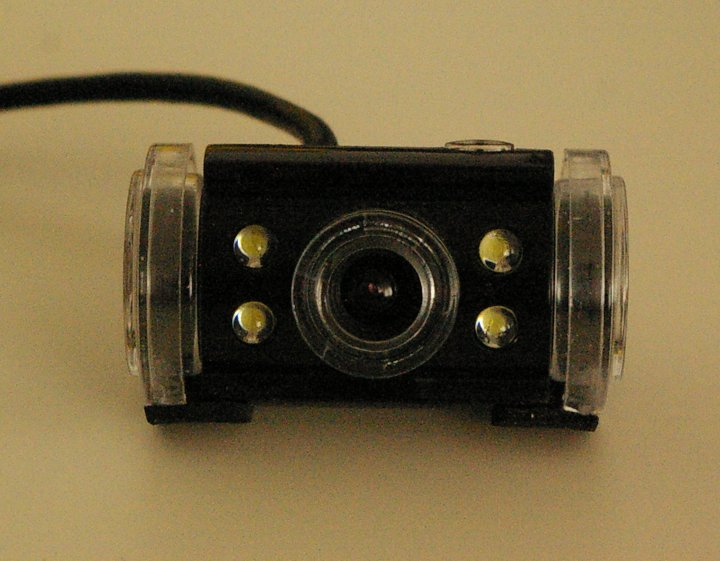
\includegraphics[height=4cm]{imagenes/camara_empleada.jpg}
	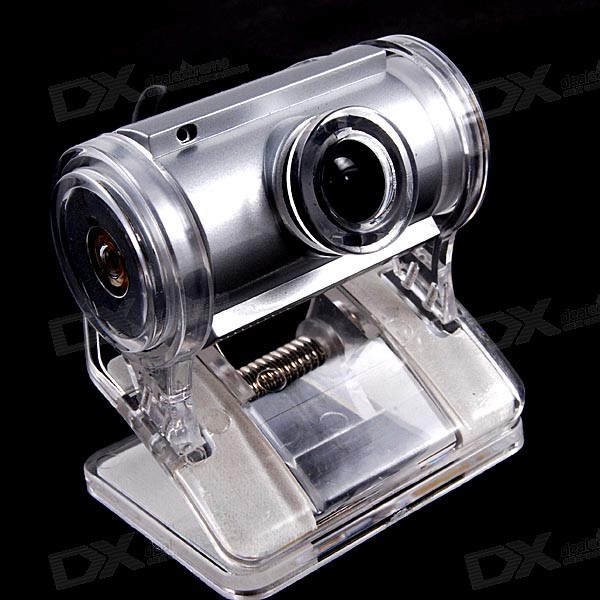
\includegraphics[height=4cm]{imagenes/camara_actual.jpg}
	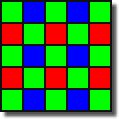
\includegraphics[height=4cm]{imagenes/bayer_mosaic.png}
        \caption{Dispositivo de captura}
	\label{fig:webcam}
\end{figure}

En cuanto a la webcam, se eligió uno de los modelos más económicos que se encontraron. El fabricante comentaba que la cámara tenía 1.3 Megapíxeles, pero se debe tener en cuenta que los fabricantes indican el número de slots que tiene el sensor CMOS como megapíxels. Por cada 4 slots del sensor CMOS (agrupados en grupos de rojo, verde, verde, azul) tenemos un píxel real \footnote{Empleando la interpolación de Bayer, obtenemos un valor BGR de 3 bytes por cada píxel, que luego se convierte a RGB vía software para mostrar por pantalla.} con lo que la resolución real de la cámara es de unos 0,3 megapíxels. Por consiguiente, el tamaño del frame es de 640x480=307200 píxeles de 3 bytes cada uno (para cada uno de los colores indicados). 

En cuanto al resto de las características de la cámara, comentar que tiene incorporado un micrófono que no se ha empleado en ningún momento y que en teoría no ha afectado al desarrollo del proyecto. También hay que tener en cuenta que dicha cámara disponía de iluminación propia (4 leds) que, aunque bastante molesta, daban unas condiciones bastante homogéneas en cuanto a iluminación a costa de en muchos momentos sobreexponer la imagen. Se optó por hacer la mayoría de las pruebas tapando dichos leds con cinta aislante por las molestias que causaban. Actualmente el fabricante ha conservado el soporte de la cámara pero ha retirado los LEDs. También se modificó el soporte de la cámara, recortando y limando el soporte de sujección/pinza que tenía debido a que hacía más complicado el uso de ella. En la figura \ref{fig:webcam} se pueden ver, de izquierda a derecha, la cámara que se ha empleado para hacer las pruebas, el modelo que distribuye actualmente el vendedor (nótese la ausencia de LEDs) y el detalle de un sensor CCD de Webcam económica, donde cada cuadrado 2x2 (colores verde-azul-rojo-verde) corresponde a un píxel.

\subsection{Escenario}
\begin{figure}[h!]
        \centering
        % Graphic for TeX using PGF
% Title: /home/bruno/pfc_UOC/PAC3/pac3/diagramas/Pasos_sistema.dia
% Creator: Dia v0.97
% CreationDate: Thu Apr 22 17:43:32 2010
% For: bruno
% \usepackage{tikz}
% The following commands are not supported in PSTricks at present
% We define them conditionally, so when they are implemented,
% this pgf file will use them.
\ifx\du\undefined
  \newlength{\du}
\fi
\setlength{\du}{15\unitlength}
\begin{tikzpicture}
\pgftransformxscale{1.000000}
\pgftransformyscale{-1.000000}
\definecolor{dialinecolor}{rgb}{0.000000, 0.000000, 0.000000}
\pgfsetstrokecolor{dialinecolor}
\definecolor{dialinecolor}{rgb}{1.000000, 1.000000, 1.000000}
\pgfsetfillcolor{dialinecolor}
\pgfsetlinewidth{0.100000\du}
\pgfsetdash{}{0pt}
\pgfsetdash{}{0pt}
\pgfsetroundjoin
{\pgfsetcornersarced{\pgfpoint{0.300000\du}{0.300000\du}}\definecolor{dialinecolor}{rgb}{0.960784, 0.980392, 0.764706}
\pgfsetfillcolor{dialinecolor}
\fill (3.600000\du,1.200000\du)--(3.600000\du,6.400000\du)--(9.700000\du,6.400000\du)--(9.700000\du,1.200000\du)--cycle;
}{\pgfsetcornersarced{\pgfpoint{0.300000\du}{0.300000\du}}\definecolor{dialinecolor}{rgb}{0.000000, 0.000000, 0.000000}
\pgfsetstrokecolor{dialinecolor}
\draw (3.600000\du,1.200000\du)--(3.600000\du,6.400000\du)--(9.700000\du,6.400000\du)--(9.700000\du,1.200000\du)--cycle;
}\pgfsetlinewidth{0.100000\du}
\pgfsetdash{}{0pt}
\pgfsetdash{}{0pt}
\pgfsetbuttcap
\pgfsetmiterjoin
\pgfsetbuttcap
\pgfsetmiterjoin
\pgfsetdash{}{0pt}
\definecolor{dialinecolor}{rgb}{0.266667, 0.266667, 0.266667}
\pgfsetstrokecolor{dialinecolor}
\pgfpathmoveto{\pgfpoint{7.697270\du}{2.515137\du}}
\pgfpathlineto{\pgfpoint{7.701699\du}{2.535068\du}}
\pgfpathlineto{\pgfpoint{7.707491\du}{2.554828\du}}
\pgfpathlineto{\pgfpoint{7.713793\du}{2.574589\du}}
\pgfpathlineto{\pgfpoint{7.721800\du}{2.594009\du}}
\pgfpathlineto{\pgfpoint{7.730317\du}{2.612406\du}}
\pgfpathlineto{\pgfpoint{7.740027\du}{2.630975\du}}
\pgfpathlineto{\pgfpoint{7.751100\du}{2.648861\du}}
\pgfpathlineto{\pgfpoint{7.762343\du}{2.666237\du}}
\pgfpathlineto{\pgfpoint{7.775119\du}{2.683102\du}}
\pgfpathlineto{\pgfpoint{7.789258\du}{2.699455\du}}
\pgfpathlineto{\pgfpoint{7.803227\du}{2.714957\du}}
\pgfpathlineto{\pgfpoint{7.819069\du}{2.729777\du}}
\pgfpathlineto{\pgfpoint{7.834571\du}{2.744087\du}}
\pgfpathlineto{\pgfpoint{7.852117\du}{2.757204\du}}
\pgfpathlineto{\pgfpoint{7.869323\du}{2.769980\du}}
\pgfpathlineto{\pgfpoint{7.887720\du}{2.781904\du}}
\pgfpathlineto{\pgfpoint{7.906970\du}{2.792807\du}}
\pgfpathlineto{\pgfpoint{7.926730\du}{2.802687\du}}
\pgfpathlineto{\pgfpoint{7.946661\du}{2.812056\du}}
\pgfpathlineto{\pgfpoint{7.967274\du}{2.820233\du}}
\pgfpathlineto{\pgfpoint{7.987886\du}{2.827388\du}}
\pgfpathlineto{\pgfpoint{8.009691\du}{2.833861\du}}
\pgfpathlineto{\pgfpoint{8.031325\du}{2.839142\du}}
\pgfpathlineto{\pgfpoint{8.053470\du}{2.843400\du}}
\pgfpathlineto{\pgfpoint{8.075445\du}{2.846637\du}}
\pgfpathlineto{\pgfpoint{8.097932\du}{2.849192\du}}
\pgfpathlineto{\pgfpoint{8.120588\du}{2.850214\du}}
\pgfpathlineto{\pgfpoint{8.142904\du}{2.850555\du}}
\pgfpathlineto{\pgfpoint{8.165390\du}{2.849533\du}}
\pgfpathlineto{\pgfpoint{8.187535\du}{2.847489\du}}
\pgfpathlineto{\pgfpoint{8.210022\du}{2.844934\du}}
\pgfpathlineto{\pgfpoint{8.232337\du}{2.841186\du}}
\pgfpathlineto{\pgfpoint{8.253631\du}{2.836246\du}}
\pgfpathlineto{\pgfpoint{8.275095\du}{2.830283\du}}
\pgfpathlineto{\pgfpoint{8.296218\du}{2.823129\du}}
\pgfpathlineto{\pgfpoint{8.317171\du}{2.815633\du}}
\pgfpathlineto{\pgfpoint{8.337784\du}{2.806946\du}}
\pgfpathlineto{\pgfpoint{8.357544\du}{2.797065\du}}
\pgfpathlineto{\pgfpoint{8.376453\du}{2.786504\du}}
\pgfpathlineto{\pgfpoint{8.395362\du}{2.775090\du}}
\pgfpathlineto{\pgfpoint{8.413249\du}{2.762825\du}}
\pgfpathlineto{\pgfpoint{8.430624\du}{2.749708\du}}
\pgfpathlineto{\pgfpoint{8.447148\du}{2.735739\du}}
\pgfpathlineto{\pgfpoint{8.462650\du}{2.721260\du}}
\pgfpathlineto{\pgfpoint{8.477641\du}{2.705928\du}}
\pgfpathlineto{\pgfpoint{8.491780\du}{2.689915\du}}
\pgfpathlineto{\pgfpoint{8.504897\du}{2.673562\du}}
\pgfpathlineto{\pgfpoint{8.516991\du}{2.656357\du}}
\pgfpathlineto{\pgfpoint{8.528405\du}{2.638470\du}}
\pgfpathlineto{\pgfpoint{8.537944\du}{2.620413\du}}
\pgfpathlineto{\pgfpoint{8.547654\du}{2.601504\du}}
\pgfpathlineto{\pgfpoint{8.556001\du}{2.582936\du}}
\pgfpathlineto{\pgfpoint{8.562645\du}{2.563175\du}}
\pgfpathlineto{\pgfpoint{8.568948\du}{2.543585\du}}
\pgfpathlineto{\pgfpoint{8.573718\du}{2.523825\du}}
\pgfusepath{stroke}
\pgfsetlinewidth{0.030000\du}
\pgfsetbuttcap
\pgfsetmiterjoin
\pgfsetdash{}{0pt}
\definecolor{dialinecolor}{rgb}{0.133333, 0.133333, 0.133333}
\pgfsetfillcolor{dialinecolor}
\pgfpathmoveto{\pgfpoint{8.516480\du}{2.379879\du}}
\pgfpathlineto{\pgfpoint{8.515799\du}{2.360630\du}}
\pgfpathlineto{\pgfpoint{8.514606\du}{2.341380\du}}
\pgfpathlineto{\pgfpoint{8.512051\du}{2.322472\du}}
\pgfpathlineto{\pgfpoint{8.508474\du}{2.303392\du}}
\pgfpathlineto{\pgfpoint{8.504045\du}{2.284484\du}}
\pgfpathlineto{\pgfpoint{8.498934\du}{2.266086\du}}
\pgfpathlineto{\pgfpoint{8.492802\du}{2.247859\du}}
\pgfpathlineto{\pgfpoint{8.485477\du}{2.229972\du}}
\pgfpathlineto{\pgfpoint{8.477470\du}{2.212767\du}}
\pgfpathlineto{\pgfpoint{8.468612\du}{2.195561\du}}
\pgfpathlineto{\pgfpoint{8.458902\du}{2.178867\du}}
\pgfpathlineto{\pgfpoint{8.448341\du}{2.162854\du}}
\pgfpathlineto{\pgfpoint{8.436757\du}{2.147352\du}}
\pgfpathlineto{\pgfpoint{8.424662\du}{2.132532\du}}
\pgfpathlineto{\pgfpoint{8.411545\du}{2.118052\du}}
\pgfpathlineto{\pgfpoint{8.398258\du}{2.104424\du}}
\pgfpathlineto{\pgfpoint{8.383778\du}{2.091478\du}}
\pgfpathlineto{\pgfpoint{8.368787\du}{2.079553\du}}
\pgfpathlineto{\pgfpoint{8.353456\du}{2.067969\du}}
\pgfpathlineto{\pgfpoint{8.337613\du}{2.057408\du}}
\pgfpathlineto{\pgfpoint{8.320749\du}{2.047868\du}}
\pgfpathlineto{\pgfpoint{8.303714\du}{2.039010\du}}
\pgfpathlineto{\pgfpoint{8.286338\du}{2.030833\du}}
\pgfpathlineto{\pgfpoint{8.268622\du}{2.023508\du}}
\pgfpathlineto{\pgfpoint{8.250224\du}{2.017205\du}}
\pgfpathlineto{\pgfpoint{8.231656\du}{2.012265\du}}
\pgfpathlineto{\pgfpoint{8.213088\du}{2.007666\du}}
\pgfpathlineto{\pgfpoint{8.194009\du}{2.004259\du}}
\pgfpathlineto{\pgfpoint{8.174930\du}{2.001874\du}}
\pgfpathlineto{\pgfpoint{8.155680\du}{2.000511\du}}
\pgfpathlineto{\pgfpoint{8.136601\du}{2.000000\du}}
\pgfpathlineto{\pgfpoint{8.136601\du}{2.000000\du}}
\pgfpathlineto{\pgfpoint{8.117351\du}{2.000511\du}}
\pgfpathlineto{\pgfpoint{8.098102\du}{2.001874\du}}
\pgfpathlineto{\pgfpoint{8.079023\du}{2.004259\du}}
\pgfpathlineto{\pgfpoint{8.059944\du}{2.007666\du}}
\pgfpathlineto{\pgfpoint{8.041035\du}{2.012265\du}}
\pgfpathlineto{\pgfpoint{8.022637\du}{2.017205\du}}
\pgfpathlineto{\pgfpoint{8.004580\du}{2.023508\du}}
\pgfpathlineto{\pgfpoint{7.986523\du}{2.030833\du}}
\pgfpathlineto{\pgfpoint{7.969147\du}{2.039010\du}}
\pgfpathlineto{\pgfpoint{7.952112\du}{2.047868\du}}
\pgfpathlineto{\pgfpoint{7.935248\du}{2.057408\du}}
\pgfpathlineto{\pgfpoint{7.919405\du}{2.067969\du}}
\pgfpathlineto{\pgfpoint{7.904074\du}{2.079553\du}}
\pgfpathlineto{\pgfpoint{7.889083\du}{2.091478\du}}
\pgfpathlineto{\pgfpoint{7.874603\du}{2.104424\du}}
\pgfpathlineto{\pgfpoint{7.861146\du}{2.118052\du}}
\pgfpathlineto{\pgfpoint{7.848199\du}{2.132532\du}}
\pgfpathlineto{\pgfpoint{7.836275\du}{2.147352\du}}
\pgfpathlineto{\pgfpoint{7.824521\du}{2.162854\du}}
\pgfpathlineto{\pgfpoint{7.814129\du}{2.178867\du}}
\pgfpathlineto{\pgfpoint{7.804419\du}{2.195561\du}}
\pgfpathlineto{\pgfpoint{7.795391\du}{2.212767\du}}
\pgfpathlineto{\pgfpoint{7.787384\du}{2.229972\du}}
\pgfpathlineto{\pgfpoint{7.780230\du}{2.247859\du}}
\pgfpathlineto{\pgfpoint{7.773927\du}{2.266086\du}}
\pgfpathlineto{\pgfpoint{7.768646\du}{2.284484\du}}
\pgfpathlineto{\pgfpoint{7.764387\du}{2.303392\du}}
\pgfpathlineto{\pgfpoint{7.761151\du}{2.322472\du}}
\pgfpathlineto{\pgfpoint{7.758595\du}{2.341380\du}}
\pgfpathlineto{\pgfpoint{7.756892\du}{2.360630\du}}
\pgfpathlineto{\pgfpoint{7.756551\du}{2.379879\du}}
\pgfpathlineto{\pgfpoint{7.756551\du}{2.379879\du}}
\pgfpathlineto{\pgfpoint{7.756892\du}{2.399129\du}}
\pgfpathlineto{\pgfpoint{7.758595\du}{2.418378\du}}
\pgfpathlineto{\pgfpoint{7.761151\du}{2.437287\du}}
\pgfpathlineto{\pgfpoint{7.764387\du}{2.456366\du}}
\pgfpathlineto{\pgfpoint{7.768646\du}{2.474934\du}}
\pgfpathlineto{\pgfpoint{7.773927\du}{2.493673\du}}
\pgfpathlineto{\pgfpoint{7.780230\du}{2.511900\du}}
\pgfpathlineto{\pgfpoint{7.787384\du}{2.529787\du}}
\pgfpathlineto{\pgfpoint{7.795391\du}{2.547163\du}}
\pgfpathlineto{\pgfpoint{7.804419\du}{2.564198\du}}
\pgfpathlineto{\pgfpoint{7.814129\du}{2.580892\du}}
\pgfpathlineto{\pgfpoint{7.824521\du}{2.596734\du}}
\pgfpathlineto{\pgfpoint{7.836275\du}{2.612406\du}}
\pgfpathlineto{\pgfpoint{7.848199\du}{2.627057\du}}
\pgfpathlineto{\pgfpoint{7.861146\du}{2.641536\du}}
\pgfpathlineto{\pgfpoint{7.874603\du}{2.654994\du}}
\pgfpathlineto{\pgfpoint{7.889083\du}{2.668111\du}}
\pgfpathlineto{\pgfpoint{7.904074\du}{2.680206\du}}
\pgfpathlineto{\pgfpoint{7.919405\du}{2.691789\du}}
\pgfpathlineto{\pgfpoint{7.935248\du}{2.702351\du}}
\pgfpathlineto{\pgfpoint{7.952112\du}{2.711891\du}}
\pgfpathlineto{\pgfpoint{7.969147\du}{2.720749\du}}
\pgfpathlineto{\pgfpoint{7.986523\du}{2.729096\du}}
\pgfpathlineto{\pgfpoint{8.004580\du}{2.735910\du}}
\pgfpathlineto{\pgfpoint{8.022637\du}{2.742213\du}}
\pgfpathlineto{\pgfpoint{8.041035\du}{2.747494\du}}
\pgfpathlineto{\pgfpoint{8.059944\du}{2.752093\du}}
\pgfpathlineto{\pgfpoint{8.079023\du}{2.755330\du}}
\pgfpathlineto{\pgfpoint{8.098102\du}{2.757885\du}}
\pgfpathlineto{\pgfpoint{8.117351\du}{2.759077\du}}
\pgfpathlineto{\pgfpoint{8.136601\du}{2.759759\du}}
\pgfpathlineto{\pgfpoint{8.136601\du}{2.759759\du}}
\pgfpathlineto{\pgfpoint{8.155680\du}{2.759077\du}}
\pgfpathlineto{\pgfpoint{8.174930\du}{2.757885\du}}
\pgfpathlineto{\pgfpoint{8.194009\du}{2.755330\du}}
\pgfpathlineto{\pgfpoint{8.213088\du}{2.752093\du}}
\pgfpathlineto{\pgfpoint{8.231656\du}{2.747494\du}}
\pgfpathlineto{\pgfpoint{8.250224\du}{2.742213\du}}
\pgfpathlineto{\pgfpoint{8.268622\du}{2.735910\du}}
\pgfpathlineto{\pgfpoint{8.286338\du}{2.729096\du}}
\pgfpathlineto{\pgfpoint{8.303714\du}{2.720749\du}}
\pgfpathlineto{\pgfpoint{8.320749\du}{2.711891\du}}
\pgfpathlineto{\pgfpoint{8.337613\du}{2.702351\du}}
\pgfpathlineto{\pgfpoint{8.353456\du}{2.691789\du}}
\pgfpathlineto{\pgfpoint{8.368787\du}{2.680206\du}}
\pgfpathlineto{\pgfpoint{8.383778\du}{2.668111\du}}
\pgfpathlineto{\pgfpoint{8.398258\du}{2.654994\du}}
\pgfpathlineto{\pgfpoint{8.411545\du}{2.641536\du}}
\pgfpathlineto{\pgfpoint{8.424662\du}{2.627057\du}}
\pgfpathlineto{\pgfpoint{8.436757\du}{2.612406\du}}
\pgfpathlineto{\pgfpoint{8.448341\du}{2.596734\du}}
\pgfpathlineto{\pgfpoint{8.458902\du}{2.580892\du}}
\pgfpathlineto{\pgfpoint{8.468612\du}{2.564198\du}}
\pgfpathlineto{\pgfpoint{8.477470\du}{2.547163\du}}
\pgfpathlineto{\pgfpoint{8.485477\du}{2.529787\du}}
\pgfpathlineto{\pgfpoint{8.492802\du}{2.511900\du}}
\pgfpathlineto{\pgfpoint{8.498934\du}{2.493673\du}}
\pgfpathlineto{\pgfpoint{8.504045\du}{2.474934\du}}
\pgfpathlineto{\pgfpoint{8.508474\du}{2.456366\du}}
\pgfpathlineto{\pgfpoint{8.512051\du}{2.437287\du}}
\pgfpathlineto{\pgfpoint{8.514606\du}{2.418378\du}}
\pgfpathlineto{\pgfpoint{8.515799\du}{2.399129\du}}
\pgfpathlineto{\pgfpoint{8.516480\du}{2.379879\du}}
\pgfusepath{fill}
\pgfsetbuttcap
\pgfsetmiterjoin
\pgfsetdash{}{0pt}
\definecolor{dialinecolor}{rgb}{0.223529, 0.223529, 0.223529}
\pgfsetfillcolor{dialinecolor}
\pgfpathmoveto{\pgfpoint{8.507963\du}{2.371532\du}}
\pgfpathlineto{\pgfpoint{8.507281\du}{2.352964\du}}
\pgfpathlineto{\pgfpoint{8.506089\du}{2.334737\du}}
\pgfpathlineto{\pgfpoint{8.503704\du}{2.316169\du}}
\pgfpathlineto{\pgfpoint{8.500467\du}{2.298112\du}}
\pgfpathlineto{\pgfpoint{8.496209\du}{2.280055\du}}
\pgfpathlineto{\pgfpoint{8.491269\du}{2.262679\du}}
\pgfpathlineto{\pgfpoint{8.485306\du}{2.245303\du}}
\pgfpathlineto{\pgfpoint{8.478322\du}{2.228268\du}}
\pgfpathlineto{\pgfpoint{8.470827\du}{2.211233\du}}
\pgfpathlineto{\pgfpoint{8.462309\du}{2.194880\du}}
\pgfpathlineto{\pgfpoint{8.452770\du}{2.179037\du}}
\pgfpathlineto{\pgfpoint{8.442889\du}{2.163876\du}}
\pgfpathlineto{\pgfpoint{8.431817\du}{2.148885\du}}
\pgfpathlineto{\pgfpoint{8.420403\du}{2.134576\du}}
\pgfpathlineto{\pgfpoint{8.407968\du}{2.121118\du}}
\pgfpathlineto{\pgfpoint{8.395021\du}{2.108172\du}}
\pgfpathlineto{\pgfpoint{8.381393\du}{2.095736\du}}
\pgfpathlineto{\pgfpoint{8.366913\du}{2.083982\du}}
\pgfpathlineto{\pgfpoint{8.352263\du}{2.073250\du}}
\pgfpathlineto{\pgfpoint{8.336762\du}{2.063029\du}}
\pgfpathlineto{\pgfpoint{8.320749\du}{2.053660\du}}
\pgfpathlineto{\pgfpoint{8.304566\du}{2.045143\du}}
\pgfpathlineto{\pgfpoint{8.287871\du}{2.037307\du}}
\pgfpathlineto{\pgfpoint{8.270666\du}{2.030493\du}}
\pgfpathlineto{\pgfpoint{8.253631\du}{2.024530\du}}
\pgfpathlineto{\pgfpoint{8.235574\du}{2.019249\du}}
\pgfpathlineto{\pgfpoint{8.217517\du}{2.015502\du}}
\pgfpathlineto{\pgfpoint{8.199630\du}{2.012265\du}}
\pgfpathlineto{\pgfpoint{8.181232\du}{2.009710\du}}
\pgfpathlineto{\pgfpoint{8.163175\du}{2.008517\du}}
\pgfpathlineto{\pgfpoint{8.144778\du}{2.008006\du}}
\pgfpathlineto{\pgfpoint{8.144778\du}{2.008006\du}}
\pgfpathlineto{\pgfpoint{8.126039\du}{2.008517\du}}
\pgfpathlineto{\pgfpoint{8.107812\du}{2.009710\du}}
\pgfpathlineto{\pgfpoint{8.089755\du}{2.012265\du}}
\pgfpathlineto{\pgfpoint{8.071698\du}{2.015502\du}}
\pgfpathlineto{\pgfpoint{8.053470\du}{2.019249\du}}
\pgfpathlineto{\pgfpoint{8.035754\du}{2.024530\du}}
\pgfpathlineto{\pgfpoint{8.018378\du}{2.030493\du}}
\pgfpathlineto{\pgfpoint{8.001343\du}{2.037307\du}}
\pgfpathlineto{\pgfpoint{7.984649\du}{2.045143\du}}
\pgfpathlineto{\pgfpoint{7.968296\du}{2.053660\du}}
\pgfpathlineto{\pgfpoint{7.952453\du}{2.063029\du}}
\pgfpathlineto{\pgfpoint{7.937122\du}{2.073250\du}}
\pgfpathlineto{\pgfpoint{7.922301\du}{2.083982\du}}
\pgfpathlineto{\pgfpoint{7.907992\du}{2.095736\du}}
\pgfpathlineto{\pgfpoint{7.894534\du}{2.108172\du}}
\pgfpathlineto{\pgfpoint{7.881247\du}{2.121118\du}}
\pgfpathlineto{\pgfpoint{7.868982\du}{2.134576\du}}
\pgfpathlineto{\pgfpoint{7.857568\du}{2.148885\du}}
\pgfpathlineto{\pgfpoint{7.846496\du}{2.163876\du}}
\pgfpathlineto{\pgfpoint{7.836275\du}{2.179037\du}}
\pgfpathlineto{\pgfpoint{7.826906\du}{2.194880\du}}
\pgfpathlineto{\pgfpoint{7.818558\du}{2.211233\du}}
\pgfpathlineto{\pgfpoint{7.810722\du}{2.228268\du}}
\pgfpathlineto{\pgfpoint{7.804079\du}{2.245303\du}}
\pgfpathlineto{\pgfpoint{7.797946\du}{2.262679\du}}
\pgfpathlineto{\pgfpoint{7.793176\du}{2.280055\du}}
\pgfpathlineto{\pgfpoint{7.788918\du}{2.298112\du}}
\pgfpathlineto{\pgfpoint{7.785681\du}{2.316169\du}}
\pgfpathlineto{\pgfpoint{7.783126\du}{2.334737\du}}
\pgfpathlineto{\pgfpoint{7.781933\du}{2.352964\du}}
\pgfpathlineto{\pgfpoint{7.781422\du}{2.371532\du}}
\pgfpathlineto{\pgfpoint{7.781422\du}{2.371532\du}}
\pgfpathlineto{\pgfpoint{7.781933\du}{2.389760\du}}
\pgfpathlineto{\pgfpoint{7.783126\du}{2.408328\du}}
\pgfpathlineto{\pgfpoint{7.785681\du}{2.426555\du}}
\pgfpathlineto{\pgfpoint{7.788918\du}{2.444612\du}}
\pgfpathlineto{\pgfpoint{7.793176\du}{2.462669\du}}
\pgfpathlineto{\pgfpoint{7.797946\du}{2.480215\du}}
\pgfpathlineto{\pgfpoint{7.804079\du}{2.497421\du}}
\pgfpathlineto{\pgfpoint{7.810722\du}{2.514796\du}}
\pgfpathlineto{\pgfpoint{7.818558\du}{2.531490\du}}
\pgfpathlineto{\pgfpoint{7.826906\du}{2.547844\du}}
\pgfpathlineto{\pgfpoint{7.836275\du}{2.563686\du}}
\pgfpathlineto{\pgfpoint{7.846496\du}{2.579018\du}}
\pgfpathlineto{\pgfpoint{7.857568\du}{2.594009\du}}
\pgfpathlineto{\pgfpoint{7.868982\du}{2.608148\du}}
\pgfpathlineto{\pgfpoint{7.881247\du}{2.621776\du}}
\pgfpathlineto{\pgfpoint{7.894534\du}{2.634552\du}}
\pgfpathlineto{\pgfpoint{7.907992\du}{2.647158\du}}
\pgfpathlineto{\pgfpoint{7.922301\du}{2.658912\du}}
\pgfpathlineto{\pgfpoint{7.937122\du}{2.669644\du}}
\pgfpathlineto{\pgfpoint{7.952453\du}{2.679865\du}}
\pgfpathlineto{\pgfpoint{7.968296\du}{2.689064\du}}
\pgfpathlineto{\pgfpoint{7.984649\du}{2.697922\du}}
\pgfpathlineto{\pgfpoint{8.001343\du}{2.705417\du}}
\pgfpathlineto{\pgfpoint{8.018378\du}{2.712231\du}}
\pgfpathlineto{\pgfpoint{8.035754\du}{2.718193\du}}
\pgfpathlineto{\pgfpoint{8.053470\du}{2.723474\du}}
\pgfpathlineto{\pgfpoint{8.071698\du}{2.727222\du}}
\pgfpathlineto{\pgfpoint{8.089755\du}{2.730459\du}}
\pgfpathlineto{\pgfpoint{8.107812\du}{2.733014\du}}
\pgfpathlineto{\pgfpoint{8.126039\du}{2.734377\du}}
\pgfpathlineto{\pgfpoint{8.144778\du}{2.734717\du}}
\pgfpathlineto{\pgfpoint{8.144778\du}{2.734717\du}}
\pgfpathlineto{\pgfpoint{8.163175\du}{2.734377\du}}
\pgfpathlineto{\pgfpoint{8.181232\du}{2.733014\du}}
\pgfpathlineto{\pgfpoint{8.199630\du}{2.730459\du}}
\pgfpathlineto{\pgfpoint{8.217517\du}{2.727222\du}}
\pgfpathlineto{\pgfpoint{8.235574\du}{2.723474\du}}
\pgfpathlineto{\pgfpoint{8.253631\du}{2.718193\du}}
\pgfpathlineto{\pgfpoint{8.270666\du}{2.712231\du}}
\pgfpathlineto{\pgfpoint{8.287871\du}{2.705417\du}}
\pgfpathlineto{\pgfpoint{8.304566\du}{2.697922\du}}
\pgfpathlineto{\pgfpoint{8.320749\du}{2.689064\du}}
\pgfpathlineto{\pgfpoint{8.336762\du}{2.679865\du}}
\pgfpathlineto{\pgfpoint{8.352263\du}{2.669644\du}}
\pgfpathlineto{\pgfpoint{8.366913\du}{2.658912\du}}
\pgfpathlineto{\pgfpoint{8.381393\du}{2.647158\du}}
\pgfpathlineto{\pgfpoint{8.395021\du}{2.634552\du}}
\pgfpathlineto{\pgfpoint{8.407968\du}{2.621776\du}}
\pgfpathlineto{\pgfpoint{8.420403\du}{2.608148\du}}
\pgfpathlineto{\pgfpoint{8.431817\du}{2.594009\du}}
\pgfpathlineto{\pgfpoint{8.442889\du}{2.579018\du}}
\pgfpathlineto{\pgfpoint{8.452770\du}{2.563686\du}}
\pgfpathlineto{\pgfpoint{8.462309\du}{2.547844\du}}
\pgfpathlineto{\pgfpoint{8.470827\du}{2.531490\du}}
\pgfpathlineto{\pgfpoint{8.478322\du}{2.514796\du}}
\pgfpathlineto{\pgfpoint{8.485306\du}{2.497421\du}}
\pgfpathlineto{\pgfpoint{8.491269\du}{2.480215\du}}
\pgfpathlineto{\pgfpoint{8.496209\du}{2.462669\du}}
\pgfpathlineto{\pgfpoint{8.500467\du}{2.444612\du}}
\pgfpathlineto{\pgfpoint{8.503704\du}{2.426555\du}}
\pgfpathlineto{\pgfpoint{8.506089\du}{2.408328\du}}
\pgfpathlineto{\pgfpoint{8.507281\du}{2.389760\du}}
\pgfpathlineto{\pgfpoint{8.507963\du}{2.371532\du}}
\pgfusepath{fill}
\pgfsetbuttcap
\pgfsetmiterjoin
\pgfsetdash{}{0pt}
\definecolor{dialinecolor}{rgb}{0.317647, 0.317647, 0.317647}
\pgfsetfillcolor{dialinecolor}
\pgfpathmoveto{\pgfpoint{8.499616\du}{2.358926\du}}
\pgfpathlineto{\pgfpoint{8.498934\du}{2.341721\du}}
\pgfpathlineto{\pgfpoint{8.497572\du}{2.324345\du}}
\pgfpathlineto{\pgfpoint{8.495357\du}{2.307140\du}}
\pgfpathlineto{\pgfpoint{8.492461\du}{2.290105\du}}
\pgfpathlineto{\pgfpoint{8.488543\du}{2.273241\du}}
\pgfpathlineto{\pgfpoint{8.483603\du}{2.256376\du}}
\pgfpathlineto{\pgfpoint{8.477981\du}{2.239682\du}}
\pgfpathlineto{\pgfpoint{8.471508\du}{2.223499\du}}
\pgfpathlineto{\pgfpoint{8.464183\du}{2.207826\du}}
\pgfpathlineto{\pgfpoint{8.456006\du}{2.192495\du}}
\pgfpathlineto{\pgfpoint{8.447148\du}{2.177675\du}}
\pgfpathlineto{\pgfpoint{8.437608\du}{2.163024\du}}
\pgfpathlineto{\pgfpoint{8.427047\du}{2.149056\du}}
\pgfpathlineto{\pgfpoint{8.415804\du}{2.135769\du}}
\pgfpathlineto{\pgfpoint{8.403879\du}{2.122992\du}}
\pgfpathlineto{\pgfpoint{8.391614\du}{2.110557\du}}
\pgfpathlineto{\pgfpoint{8.378838\du}{2.098973\du}}
\pgfpathlineto{\pgfpoint{8.365210\du}{2.087900\du}}
\pgfpathlineto{\pgfpoint{8.350730\du}{2.077679\du}}
\pgfpathlineto{\pgfpoint{8.336251\du}{2.067969\du}}
\pgfpathlineto{\pgfpoint{8.321089\du}{2.059452\du}}
\pgfpathlineto{\pgfpoint{8.305588\du}{2.051105\du}}
\pgfpathlineto{\pgfpoint{8.289575\du}{2.043780\du}}
\pgfpathlineto{\pgfpoint{8.273051\du}{2.037307\du}}
\pgfpathlineto{\pgfpoint{8.256527\du}{2.031855\du}}
\pgfpathlineto{\pgfpoint{8.239833\du}{2.027256\du}}
\pgfpathlineto{\pgfpoint{8.222627\du}{2.023338\du}}
\pgfpathlineto{\pgfpoint{8.205422\du}{2.020101\du}}
\pgfpathlineto{\pgfpoint{8.187876\du}{2.018057\du}}
\pgfpathlineto{\pgfpoint{8.170500\du}{2.016694\du}}
\pgfpathlineto{\pgfpoint{8.152784\du}{2.016013\du}}
\pgfpathlineto{\pgfpoint{8.152784\du}{2.016013\du}}
\pgfpathlineto{\pgfpoint{8.135408\du}{2.016694\du}}
\pgfpathlineto{\pgfpoint{8.117692\du}{2.018057\du}}
\pgfpathlineto{\pgfpoint{8.100316\du}{2.020101\du}}
\pgfpathlineto{\pgfpoint{8.083111\du}{2.023338\du}}
\pgfpathlineto{\pgfpoint{8.066076\du}{2.027256\du}}
\pgfpathlineto{\pgfpoint{8.049212\du}{2.031855\du}}
\pgfpathlineto{\pgfpoint{8.032517\du}{2.037307\du}}
\pgfpathlineto{\pgfpoint{8.016164\du}{2.043780\du}}
\pgfpathlineto{\pgfpoint{8.000321\du}{2.051105\du}}
\pgfpathlineto{\pgfpoint{7.984479\du}{2.059452\du}}
\pgfpathlineto{\pgfpoint{7.969488\du}{2.067969\du}}
\pgfpathlineto{\pgfpoint{7.954668\du}{2.077679\du}}
\pgfpathlineto{\pgfpoint{7.940699\du}{2.087900\du}}
\pgfpathlineto{\pgfpoint{7.926901\du}{2.098973\du}}
\pgfpathlineto{\pgfpoint{7.913954\du}{2.110557\du}}
\pgfpathlineto{\pgfpoint{7.901519\du}{2.122992\du}}
\pgfpathlineto{\pgfpoint{7.889594\du}{2.135769\du}}
\pgfpathlineto{\pgfpoint{7.878862\du}{2.149056\du}}
\pgfpathlineto{\pgfpoint{7.868300\du}{2.163024\du}}
\pgfpathlineto{\pgfpoint{7.858591\du}{2.177675\du}}
\pgfpathlineto{\pgfpoint{7.849732\du}{2.192495\du}}
\pgfpathlineto{\pgfpoint{7.841556\du}{2.207826\du}}
\pgfpathlineto{\pgfpoint{7.834231\du}{2.223499\du}}
\pgfpathlineto{\pgfpoint{7.827757\du}{2.239682\du}}
\pgfpathlineto{\pgfpoint{7.822136\du}{2.256376\du}}
\pgfpathlineto{\pgfpoint{7.817196\du}{2.273241\du}}
\pgfpathlineto{\pgfpoint{7.813107\du}{2.290105\du}}
\pgfpathlineto{\pgfpoint{7.810041\du}{2.307140\du}}
\pgfpathlineto{\pgfpoint{7.808167\du}{2.324345\du}}
\pgfpathlineto{\pgfpoint{7.806634\du}{2.341721\du}}
\pgfpathlineto{\pgfpoint{7.806293\du}{2.358926\du}}
\pgfpathlineto{\pgfpoint{7.806293\du}{2.358926\du}}
\pgfpathlineto{\pgfpoint{7.806634\du}{2.376472\du}}
\pgfpathlineto{\pgfpoint{7.808167\du}{2.393678\du}}
\pgfpathlineto{\pgfpoint{7.810041\du}{2.410883\du}}
\pgfpathlineto{\pgfpoint{7.813107\du}{2.427918\du}}
\pgfpathlineto{\pgfpoint{7.817196\du}{2.444783\du}}
\pgfpathlineto{\pgfpoint{7.822136\du}{2.461817\du}}
\pgfpathlineto{\pgfpoint{7.827757\du}{2.478001\du}}
\pgfpathlineto{\pgfpoint{7.834231\du}{2.494184\du}}
\pgfpathlineto{\pgfpoint{7.841556\du}{2.510026\du}}
\pgfpathlineto{\pgfpoint{7.849732\du}{2.525528\du}}
\pgfpathlineto{\pgfpoint{7.858591\du}{2.540349\du}}
\pgfpathlineto{\pgfpoint{7.868300\du}{2.554658\du}}
\pgfpathlineto{\pgfpoint{7.878862\du}{2.568967\du}}
\pgfpathlineto{\pgfpoint{7.889594\du}{2.582255\du}}
\pgfpathlineto{\pgfpoint{7.901519\du}{2.595201\du}}
\pgfpathlineto{\pgfpoint{7.913954\du}{2.607637\du}}
\pgfpathlineto{\pgfpoint{7.926901\du}{2.619050\du}}
\pgfpathlineto{\pgfpoint{7.940699\du}{2.630123\du}}
\pgfpathlineto{\pgfpoint{7.954668\du}{2.640344\du}}
\pgfpathlineto{\pgfpoint{7.969488\du}{2.650054\du}}
\pgfpathlineto{\pgfpoint{7.984479\du}{2.658742\du}}
\pgfpathlineto{\pgfpoint{8.000321\du}{2.666918\du}}
\pgfpathlineto{\pgfpoint{8.016164\du}{2.674073\du}}
\pgfpathlineto{\pgfpoint{8.032517\du}{2.680376\du}}
\pgfpathlineto{\pgfpoint{8.049212\du}{2.686168\du}}
\pgfpathlineto{\pgfpoint{8.066076\du}{2.690767\du}}
\pgfpathlineto{\pgfpoint{8.083111\du}{2.694856\du}}
\pgfpathlineto{\pgfpoint{8.100316\du}{2.697922\du}}
\pgfpathlineto{\pgfpoint{8.117692\du}{2.699966\du}}
\pgfpathlineto{\pgfpoint{8.135408\du}{2.701329\du}}
\pgfpathlineto{\pgfpoint{8.152784\du}{2.701670\du}}
\pgfpathlineto{\pgfpoint{8.152784\du}{2.701670\du}}
\pgfpathlineto{\pgfpoint{8.170500\du}{2.701329\du}}
\pgfpathlineto{\pgfpoint{8.187876\du}{2.699966\du}}
\pgfpathlineto{\pgfpoint{8.205422\du}{2.697922\du}}
\pgfpathlineto{\pgfpoint{8.222627\du}{2.694856\du}}
\pgfpathlineto{\pgfpoint{8.239833\du}{2.690767\du}}
\pgfpathlineto{\pgfpoint{8.256527\du}{2.686168\du}}
\pgfpathlineto{\pgfpoint{8.273051\du}{2.680376\du}}
\pgfpathlineto{\pgfpoint{8.289575\du}{2.674073\du}}
\pgfpathlineto{\pgfpoint{8.305588\du}{2.666918\du}}
\pgfpathlineto{\pgfpoint{8.321089\du}{2.658742\du}}
\pgfpathlineto{\pgfpoint{8.336251\du}{2.650054\du}}
\pgfpathlineto{\pgfpoint{8.350730\du}{2.640344\du}}
\pgfpathlineto{\pgfpoint{8.365210\du}{2.630123\du}}
\pgfpathlineto{\pgfpoint{8.378838\du}{2.619050\du}}
\pgfpathlineto{\pgfpoint{8.391614\du}{2.607637\du}}
\pgfpathlineto{\pgfpoint{8.403879\du}{2.595201\du}}
\pgfpathlineto{\pgfpoint{8.415804\du}{2.582255\du}}
\pgfpathlineto{\pgfpoint{8.427047\du}{2.568967\du}}
\pgfpathlineto{\pgfpoint{8.437608\du}{2.554658\du}}
\pgfpathlineto{\pgfpoint{8.447148\du}{2.540349\du}}
\pgfpathlineto{\pgfpoint{8.456006\du}{2.525528\du}}
\pgfpathlineto{\pgfpoint{8.464183\du}{2.510026\du}}
\pgfpathlineto{\pgfpoint{8.471508\du}{2.494184\du}}
\pgfpathlineto{\pgfpoint{8.477981\du}{2.478001\du}}
\pgfpathlineto{\pgfpoint{8.483603\du}{2.461817\du}}
\pgfpathlineto{\pgfpoint{8.488543\du}{2.444783\du}}
\pgfpathlineto{\pgfpoint{8.492461\du}{2.427918\du}}
\pgfpathlineto{\pgfpoint{8.495357\du}{2.410883\du}}
\pgfpathlineto{\pgfpoint{8.497572\du}{2.393678\du}}
\pgfpathlineto{\pgfpoint{8.498934\du}{2.376472\du}}
\pgfpathlineto{\pgfpoint{8.499616\du}{2.358926\du}}
\pgfusepath{fill}
\pgfsetbuttcap
\pgfsetmiterjoin
\pgfsetdash{}{0pt}
\definecolor{dialinecolor}{rgb}{0.403922, 0.403922, 0.403922}
\pgfsetfillcolor{dialinecolor}
\pgfpathmoveto{\pgfpoint{8.483433\du}{2.346661\du}}
\pgfpathlineto{\pgfpoint{8.482751\du}{2.329967\du}}
\pgfpathlineto{\pgfpoint{8.481559\du}{2.313954\du}}
\pgfpathlineto{\pgfpoint{8.479514\du}{2.297771\du}}
\pgfpathlineto{\pgfpoint{8.476448\du}{2.281588\du}}
\pgfpathlineto{\pgfpoint{8.472871\du}{2.265916\du}}
\pgfpathlineto{\pgfpoint{8.468442\du}{2.250073\du}}
\pgfpathlineto{\pgfpoint{8.462991\du}{2.234742\du}}
\pgfpathlineto{\pgfpoint{8.457028\du}{2.219410\du}}
\pgfpathlineto{\pgfpoint{8.450214\du}{2.204590\du}}
\pgfpathlineto{\pgfpoint{8.442208\du}{2.190280\du}}
\pgfpathlineto{\pgfpoint{8.433861\du}{2.176141\du}}
\pgfpathlineto{\pgfpoint{8.424832\du}{2.162513\du}}
\pgfpathlineto{\pgfpoint{8.415122\du}{2.149226\du}}
\pgfpathlineto{\pgfpoint{8.404731\du}{2.136791\du}}
\pgfpathlineto{\pgfpoint{8.393318\du}{2.124525\du}}
\pgfpathlineto{\pgfpoint{8.381734\du}{2.112942\du}}
\pgfpathlineto{\pgfpoint{8.369639\du}{2.102039\du}}
\pgfpathlineto{\pgfpoint{8.356863\du}{2.091478\du}}
\pgfpathlineto{\pgfpoint{8.343235\du}{2.081938\du}}
\pgfpathlineto{\pgfpoint{8.329437\du}{2.073250\du}}
\pgfpathlineto{\pgfpoint{8.315468\du}{2.064903\du}}
\pgfpathlineto{\pgfpoint{8.300647\du}{2.057237\du}}
\pgfpathlineto{\pgfpoint{8.285657\du}{2.050253\du}}
\pgfpathlineto{\pgfpoint{8.270496\du}{2.044632\du}}
\pgfpathlineto{\pgfpoint{8.254653\du}{2.039180\du}}
\pgfpathlineto{\pgfpoint{8.238811\du}{2.034751\du}}
\pgfpathlineto{\pgfpoint{8.222798\du}{2.030833\du}}
\pgfpathlineto{\pgfpoint{8.206444\du}{2.028108\du}}
\pgfpathlineto{\pgfpoint{8.189920\du}{2.026063\du}}
\pgfpathlineto{\pgfpoint{8.173737\du}{2.024701\du}}
\pgfpathlineto{\pgfpoint{8.157043\du}{2.024360\du}}
\pgfpathlineto{\pgfpoint{8.157043\du}{2.024360\du}}
\pgfpathlineto{\pgfpoint{8.140519\du}{2.024701\du}}
\pgfpathlineto{\pgfpoint{8.123995\du}{2.026063\du}}
\pgfpathlineto{\pgfpoint{8.107812\du}{2.028108\du}}
\pgfpathlineto{\pgfpoint{8.091118\du}{2.030833\du}}
\pgfpathlineto{\pgfpoint{8.075445\du}{2.034751\du}}
\pgfpathlineto{\pgfpoint{8.059603\du}{2.039180\du}}
\pgfpathlineto{\pgfpoint{8.043760\du}{2.044632\du}}
\pgfpathlineto{\pgfpoint{8.028259\du}{2.050253\du}}
\pgfpathlineto{\pgfpoint{8.013268\du}{2.057237\du}}
\pgfpathlineto{\pgfpoint{7.998447\du}{2.064903\du}}
\pgfpathlineto{\pgfpoint{7.984479\du}{2.073250\du}}
\pgfpathlineto{\pgfpoint{7.970681\du}{2.081938\du}}
\pgfpathlineto{\pgfpoint{7.957393\du}{2.091478\du}}
\pgfpathlineto{\pgfpoint{7.944617\du}{2.102039\du}}
\pgfpathlineto{\pgfpoint{7.932182\du}{2.112942\du}}
\pgfpathlineto{\pgfpoint{7.920598\du}{2.124525\du}}
\pgfpathlineto{\pgfpoint{7.909525\du}{2.136791\du}}
\pgfpathlineto{\pgfpoint{7.899134\du}{2.149226\du}}
\pgfpathlineto{\pgfpoint{7.889424\du}{2.162513\du}}
\pgfpathlineto{\pgfpoint{7.880055\du}{2.176141\du}}
\pgfpathlineto{\pgfpoint{7.871707\du}{2.190280\du}}
\pgfpathlineto{\pgfpoint{7.864042\du}{2.204590\du}}
\pgfpathlineto{\pgfpoint{7.857228\du}{2.219410\du}}
\pgfpathlineto{\pgfpoint{7.851266\du}{2.234742\du}}
\pgfpathlineto{\pgfpoint{7.845814\du}{2.250073\du}}
\pgfpathlineto{\pgfpoint{7.841385\du}{2.265916\du}}
\pgfpathlineto{\pgfpoint{7.837467\du}{2.281588\du}}
\pgfpathlineto{\pgfpoint{7.834401\du}{2.297771\du}}
\pgfpathlineto{\pgfpoint{7.832357\du}{2.313954\du}}
\pgfpathlineto{\pgfpoint{7.831164\du}{2.329967\du}}
\pgfpathlineto{\pgfpoint{7.830824\du}{2.346661\du}}
\pgfpathlineto{\pgfpoint{7.830824\du}{2.346661\du}}
\pgfpathlineto{\pgfpoint{7.831164\du}{2.363015\du}}
\pgfpathlineto{\pgfpoint{7.832357\du}{2.379028\du}}
\pgfpathlineto{\pgfpoint{7.834401\du}{2.395211\du}}
\pgfpathlineto{\pgfpoint{7.837467\du}{2.411564\du}}
\pgfpathlineto{\pgfpoint{7.841385\du}{2.427066\du}}
\pgfpathlineto{\pgfpoint{7.845814\du}{2.442909\du}}
\pgfpathlineto{\pgfpoint{7.851266\du}{2.458411\du}}
\pgfpathlineto{\pgfpoint{7.857228\du}{2.473742\du}}
\pgfpathlineto{\pgfpoint{7.864042\du}{2.488562\du}}
\pgfpathlineto{\pgfpoint{7.871707\du}{2.503042\du}}
\pgfpathlineto{\pgfpoint{7.880055\du}{2.517011\du}}
\pgfpathlineto{\pgfpoint{7.889424\du}{2.530639\du}}
\pgfpathlineto{\pgfpoint{7.899134\du}{2.543756\du}}
\pgfpathlineto{\pgfpoint{7.909525\du}{2.556532\du}}
\pgfpathlineto{\pgfpoint{7.920598\du}{2.568456\du}}
\pgfpathlineto{\pgfpoint{7.932182\du}{2.580210\du}}
\pgfpathlineto{\pgfpoint{7.944617\du}{2.590942\du}}
\pgfpathlineto{\pgfpoint{7.957393\du}{2.601504\du}}
\pgfpathlineto{\pgfpoint{7.970681\du}{2.611044\du}}
\pgfpathlineto{\pgfpoint{7.984479\du}{2.620072\du}}
\pgfpathlineto{\pgfpoint{7.998447\du}{2.628079\du}}
\pgfpathlineto{\pgfpoint{8.013268\du}{2.635744\du}}
\pgfpathlineto{\pgfpoint{8.028259\du}{2.642729\du}}
\pgfpathlineto{\pgfpoint{8.043760\du}{2.648521\du}}
\pgfpathlineto{\pgfpoint{8.059603\du}{2.653801\du}}
\pgfpathlineto{\pgfpoint{8.075445\du}{2.658401\du}}
\pgfpathlineto{\pgfpoint{8.091118\du}{2.662149\du}}
\pgfpathlineto{\pgfpoint{8.107812\du}{2.665044\du}}
\pgfpathlineto{\pgfpoint{8.123995\du}{2.667089\du}}
\pgfpathlineto{\pgfpoint{8.140519\du}{2.668281\du}}
\pgfpathlineto{\pgfpoint{8.157043\du}{2.668622\du}}
\pgfpathlineto{\pgfpoint{8.157043\du}{2.668622\du}}
\pgfpathlineto{\pgfpoint{8.173737\du}{2.668281\du}}
\pgfpathlineto{\pgfpoint{8.189920\du}{2.667089\du}}
\pgfpathlineto{\pgfpoint{8.206444\du}{2.665044\du}}
\pgfpathlineto{\pgfpoint{8.222798\du}{2.662149\du}}
\pgfpathlineto{\pgfpoint{8.238811\du}{2.658401\du}}
\pgfpathlineto{\pgfpoint{8.254653\du}{2.653801\du}}
\pgfpathlineto{\pgfpoint{8.270496\du}{2.648521\du}}
\pgfpathlineto{\pgfpoint{8.285657\du}{2.642729\du}}
\pgfpathlineto{\pgfpoint{8.300647\du}{2.635744\du}}
\pgfpathlineto{\pgfpoint{8.315468\du}{2.628079\du}}
\pgfpathlineto{\pgfpoint{8.329437\du}{2.620072\du}}
\pgfpathlineto{\pgfpoint{8.343235\du}{2.611044\du}}
\pgfpathlineto{\pgfpoint{8.356863\du}{2.601504\du}}
\pgfpathlineto{\pgfpoint{8.369639\du}{2.590942\du}}
\pgfpathlineto{\pgfpoint{8.381734\du}{2.580210\du}}
\pgfpathlineto{\pgfpoint{8.393318\du}{2.568456\du}}
\pgfpathlineto{\pgfpoint{8.404731\du}{2.556532\du}}
\pgfpathlineto{\pgfpoint{8.415122\du}{2.543756\du}}
\pgfpathlineto{\pgfpoint{8.424832\du}{2.530639\du}}
\pgfpathlineto{\pgfpoint{8.433861\du}{2.517011\du}}
\pgfpathlineto{\pgfpoint{8.442208\du}{2.503042\du}}
\pgfpathlineto{\pgfpoint{8.450214\du}{2.488562\du}}
\pgfpathlineto{\pgfpoint{8.457028\du}{2.473742\du}}
\pgfpathlineto{\pgfpoint{8.462991\du}{2.458411\du}}
\pgfpathlineto{\pgfpoint{8.468442\du}{2.442909\du}}
\pgfpathlineto{\pgfpoint{8.472871\du}{2.427066\du}}
\pgfpathlineto{\pgfpoint{8.476448\du}{2.411564\du}}
\pgfpathlineto{\pgfpoint{8.479514\du}{2.395211\du}}
\pgfpathlineto{\pgfpoint{8.481559\du}{2.379028\du}}
\pgfpathlineto{\pgfpoint{8.482751\du}{2.363015\du}}
\pgfpathlineto{\pgfpoint{8.483433\du}{2.346661\du}}
\pgfusepath{fill}
\pgfsetbuttcap
\pgfsetmiterjoin
\pgfsetdash{}{0pt}
\definecolor{dialinecolor}{rgb}{0.482353, 0.482353, 0.482353}
\pgfsetfillcolor{dialinecolor}
\pgfpathmoveto{\pgfpoint{8.474915\du}{2.334226\du}}
\pgfpathlineto{\pgfpoint{8.474404\du}{2.318554\du}}
\pgfpathlineto{\pgfpoint{8.473212\du}{2.303052\du}}
\pgfpathlineto{\pgfpoint{8.471508\du}{2.287380\du}}
\pgfpathlineto{\pgfpoint{8.468612\du}{2.272048\du}}
\pgfpathlineto{\pgfpoint{8.465205\du}{2.256717\du}}
\pgfpathlineto{\pgfpoint{8.460946\du}{2.241556\du}}
\pgfpathlineto{\pgfpoint{8.456006\du}{2.226735\du}}
\pgfpathlineto{\pgfpoint{8.450214\du}{2.212085\du}}
\pgfpathlineto{\pgfpoint{8.443911\du}{2.197946\du}}
\pgfpathlineto{\pgfpoint{8.436586\du}{2.184148\du}}
\pgfpathlineto{\pgfpoint{8.428410\du}{2.170350\du}}
\pgfpathlineto{\pgfpoint{8.420062\du}{2.157403\du}}
\pgfpathlineto{\pgfpoint{8.411034\du}{2.144797\du}}
\pgfpathlineto{\pgfpoint{8.401324\du}{2.132702\du}}
\pgfpathlineto{\pgfpoint{8.390933\du}{2.121118\du}}
\pgfpathlineto{\pgfpoint{8.380030\du}{2.109875\du}}
\pgfpathlineto{\pgfpoint{8.368447\du}{2.099484\du}}
\pgfpathlineto{\pgfpoint{8.356522\du}{2.089433\du}}
\pgfpathlineto{\pgfpoint{8.344087\du}{2.080064\du}}
\pgfpathlineto{\pgfpoint{8.330970\du}{2.071376\du}}
\pgfpathlineto{\pgfpoint{8.317682\du}{2.063540\du}}
\pgfpathlineto{\pgfpoint{8.303884\du}{2.056386\du}}
\pgfpathlineto{\pgfpoint{8.289915\du}{2.049742\du}}
\pgfpathlineto{\pgfpoint{8.275606\du}{2.043780\du}}
\pgfpathlineto{\pgfpoint{8.261126\du}{2.039010\du}}
\pgfpathlineto{\pgfpoint{8.246136\du}{2.034581\du}}
\pgfpathlineto{\pgfpoint{8.231145\du}{2.030833\du}}
\pgfpathlineto{\pgfpoint{8.215643\du}{2.028108\du}}
\pgfpathlineto{\pgfpoint{8.200482\du}{2.026234\du}}
\pgfpathlineto{\pgfpoint{8.184810\du}{2.025212\du}}
\pgfpathlineto{\pgfpoint{8.169478\du}{2.024530\du}}
\pgfpathlineto{\pgfpoint{8.169478\du}{2.024530\du}}
\pgfpathlineto{\pgfpoint{8.153977\du}{2.025212\du}}
\pgfpathlineto{\pgfpoint{8.138645\du}{2.026234\du}}
\pgfpathlineto{\pgfpoint{8.122973\du}{2.028108\du}}
\pgfpathlineto{\pgfpoint{8.107812\du}{2.030833\du}}
\pgfpathlineto{\pgfpoint{8.092991\du}{2.034581\du}}
\pgfpathlineto{\pgfpoint{8.078001\du}{2.039010\du}}
\pgfpathlineto{\pgfpoint{8.063351\du}{2.043780\du}}
\pgfpathlineto{\pgfpoint{8.049041\du}{2.049742\du}}
\pgfpathlineto{\pgfpoint{8.034732\du}{2.056386\du}}
\pgfpathlineto{\pgfpoint{8.021445\du}{2.063540\du}}
\pgfpathlineto{\pgfpoint{8.007817\du}{2.071376\du}}
\pgfpathlineto{\pgfpoint{7.994870\du}{2.080064\du}}
\pgfpathlineto{\pgfpoint{7.982264\du}{2.089433\du}}
\pgfpathlineto{\pgfpoint{7.970510\du}{2.099484\du}}
\pgfpathlineto{\pgfpoint{7.958926\du}{2.109875\du}}
\pgfpathlineto{\pgfpoint{7.948024\du}{2.121118\du}}
\pgfpathlineto{\pgfpoint{7.937633\du}{2.132702\du}}
\pgfpathlineto{\pgfpoint{7.927923\du}{2.144797\du}}
\pgfpathlineto{\pgfpoint{7.918894\du}{2.157403\du}}
\pgfpathlineto{\pgfpoint{7.910377\du}{2.170350\du}}
\pgfpathlineto{\pgfpoint{7.902370\du}{2.184148\du}}
\pgfpathlineto{\pgfpoint{7.895045\du}{2.197946\du}}
\pgfpathlineto{\pgfpoint{7.888742\du}{2.212085\du}}
\pgfpathlineto{\pgfpoint{7.883121\du}{2.226735\du}}
\pgfpathlineto{\pgfpoint{7.878010\du}{2.241556\du}}
\pgfpathlineto{\pgfpoint{7.873752\du}{2.256717\du}}
\pgfpathlineto{\pgfpoint{7.870345\du}{2.272048\du}}
\pgfpathlineto{\pgfpoint{7.867449\du}{2.287380\du}}
\pgfpathlineto{\pgfpoint{7.865745\du}{2.303052\du}}
\pgfpathlineto{\pgfpoint{7.864382\du}{2.318554\du}}
\pgfpathlineto{\pgfpoint{7.864042\du}{2.334226\du}}
\pgfpathlineto{\pgfpoint{7.864042\du}{2.334226\du}}
\pgfpathlineto{\pgfpoint{7.864382\du}{2.350068\du}}
\pgfpathlineto{\pgfpoint{7.865745\du}{2.365911\du}}
\pgfpathlineto{\pgfpoint{7.867449\du}{2.381072\du}}
\pgfpathlineto{\pgfpoint{7.870345\du}{2.396744\du}}
\pgfpathlineto{\pgfpoint{7.873752\du}{2.412075\du}}
\pgfpathlineto{\pgfpoint{7.878010\du}{2.426896\du}}
\pgfpathlineto{\pgfpoint{7.883121\du}{2.441887\du}}
\pgfpathlineto{\pgfpoint{7.888742\du}{2.456537\du}}
\pgfpathlineto{\pgfpoint{7.895045\du}{2.470676\du}}
\pgfpathlineto{\pgfpoint{7.902370\du}{2.484474\du}}
\pgfpathlineto{\pgfpoint{7.910377\du}{2.498272\du}}
\pgfpathlineto{\pgfpoint{7.918894\du}{2.511219\du}}
\pgfpathlineto{\pgfpoint{7.927923\du}{2.523995\du}}
\pgfpathlineto{\pgfpoint{7.937633\du}{2.536090\du}}
\pgfpathlineto{\pgfpoint{7.948024\du}{2.547844\du}}
\pgfpathlineto{\pgfpoint{7.958926\du}{2.558746\du}}
\pgfpathlineto{\pgfpoint{7.970510\du}{2.569308\du}}
\pgfpathlineto{\pgfpoint{7.982264\du}{2.579359\du}}
\pgfpathlineto{\pgfpoint{7.994870\du}{2.588558\du}}
\pgfpathlineto{\pgfpoint{8.007817\du}{2.597245\du}}
\pgfpathlineto{\pgfpoint{8.021445\du}{2.605252\du}}
\pgfpathlineto{\pgfpoint{8.034732\du}{2.612406\du}}
\pgfpathlineto{\pgfpoint{8.049041\du}{2.619050\du}}
\pgfpathlineto{\pgfpoint{8.063351\du}{2.625012\du}}
\pgfpathlineto{\pgfpoint{8.078001\du}{2.629952\du}}
\pgfpathlineto{\pgfpoint{8.092991\du}{2.634382\du}}
\pgfpathlineto{\pgfpoint{8.107812\du}{2.637789\du}}
\pgfpathlineto{\pgfpoint{8.122973\du}{2.640684\du}}
\pgfpathlineto{\pgfpoint{8.138645\du}{2.642558\du}}
\pgfpathlineto{\pgfpoint{8.153977\du}{2.643751\du}}
\pgfpathlineto{\pgfpoint{8.169478\du}{2.644091\du}}
\pgfpathlineto{\pgfpoint{8.169478\du}{2.644091\du}}
\pgfpathlineto{\pgfpoint{8.184810\du}{2.643751\du}}
\pgfpathlineto{\pgfpoint{8.200482\du}{2.642558\du}}
\pgfpathlineto{\pgfpoint{8.215643\du}{2.640684\du}}
\pgfpathlineto{\pgfpoint{8.231145\du}{2.637789\du}}
\pgfpathlineto{\pgfpoint{8.246136\du}{2.634382\du}}
\pgfpathlineto{\pgfpoint{8.261126\du}{2.629952\du}}
\pgfpathlineto{\pgfpoint{8.275606\du}{2.625012\du}}
\pgfpathlineto{\pgfpoint{8.289915\du}{2.619050\du}}
\pgfpathlineto{\pgfpoint{8.303884\du}{2.612406\du}}
\pgfpathlineto{\pgfpoint{8.317682\du}{2.605252\du}}
\pgfpathlineto{\pgfpoint{8.330970\du}{2.597245\du}}
\pgfpathlineto{\pgfpoint{8.344087\du}{2.588558\du}}
\pgfpathlineto{\pgfpoint{8.356522\du}{2.579359\du}}
\pgfpathlineto{\pgfpoint{8.368447\du}{2.569308\du}}
\pgfpathlineto{\pgfpoint{8.380030\du}{2.558746\du}}
\pgfpathlineto{\pgfpoint{8.390933\du}{2.547844\du}}
\pgfpathlineto{\pgfpoint{8.401324\du}{2.536090\du}}
\pgfpathlineto{\pgfpoint{8.411034\du}{2.523995\du}}
\pgfpathlineto{\pgfpoint{8.420062\du}{2.511219\du}}
\pgfpathlineto{\pgfpoint{8.428410\du}{2.498272\du}}
\pgfpathlineto{\pgfpoint{8.436586\du}{2.484474\du}}
\pgfpathlineto{\pgfpoint{8.443911\du}{2.470676\du}}
\pgfpathlineto{\pgfpoint{8.450214\du}{2.456537\du}}
\pgfpathlineto{\pgfpoint{8.456006\du}{2.441887\du}}
\pgfpathlineto{\pgfpoint{8.460946\du}{2.426896\du}}
\pgfpathlineto{\pgfpoint{8.465205\du}{2.412075\du}}
\pgfpathlineto{\pgfpoint{8.468612\du}{2.396744\du}}
\pgfpathlineto{\pgfpoint{8.471508\du}{2.381072\du}}
\pgfpathlineto{\pgfpoint{8.473212\du}{2.365911\du}}
\pgfpathlineto{\pgfpoint{8.474404\du}{2.350068\du}}
\pgfpathlineto{\pgfpoint{8.474915\du}{2.334226\du}}
\pgfusepath{fill}
\pgfsetbuttcap
\pgfsetmiterjoin
\pgfsetdash{}{0pt}
\definecolor{dialinecolor}{rgb}{0.552941, 0.552941, 0.552941}
\pgfsetfillcolor{dialinecolor}
\pgfpathmoveto{\pgfpoint{8.466568\du}{2.321961\du}}
\pgfpathlineto{\pgfpoint{8.465887\du}{2.307481\du}}
\pgfpathlineto{\pgfpoint{8.465205\du}{2.292660\du}}
\pgfpathlineto{\pgfpoint{8.463331\du}{2.278010\du}}
\pgfpathlineto{\pgfpoint{8.460606\du}{2.263871\du}}
\pgfpathlineto{\pgfpoint{8.457199\du}{2.249562\du}}
\pgfpathlineto{\pgfpoint{8.453110\du}{2.235253\du}}
\pgfpathlineto{\pgfpoint{8.448511\du}{2.221454\du}}
\pgfpathlineto{\pgfpoint{8.443230\du}{2.207826\du}}
\pgfpathlineto{\pgfpoint{8.436927\du}{2.194709\du}}
\pgfpathlineto{\pgfpoint{8.430283\du}{2.181763\du}}
\pgfpathlineto{\pgfpoint{8.422788\du}{2.169157\du}}
\pgfpathlineto{\pgfpoint{8.414611\du}{2.156722\du}}
\pgfpathlineto{\pgfpoint{8.405923\du}{2.144797\du}}
\pgfpathlineto{\pgfpoint{8.396725\du}{2.133724\du}}
\pgfpathlineto{\pgfpoint{8.386844\du}{2.122992\du}}
\pgfpathlineto{\pgfpoint{8.376453\du}{2.112431\du}}
\pgfpathlineto{\pgfpoint{8.365721\du}{2.102380\du}}
\pgfpathlineto{\pgfpoint{8.354478\du}{2.093352\du}}
\pgfpathlineto{\pgfpoint{8.342724\du}{2.084664\du}}
\pgfpathlineto{\pgfpoint{8.330459\du}{2.076657\du}}
\pgfpathlineto{\pgfpoint{8.317682\du}{2.069162\du}}
\pgfpathlineto{\pgfpoint{8.304906\du}{2.062348\du}}
\pgfpathlineto{\pgfpoint{8.291789\du}{2.056386\du}}
\pgfpathlineto{\pgfpoint{8.278161\du}{2.050935\du}}
\pgfpathlineto{\pgfpoint{8.264022\du}{2.045994\du}}
\pgfpathlineto{\pgfpoint{8.250054\du}{2.042076\du}}
\pgfpathlineto{\pgfpoint{8.235574\du}{2.038499\du}}
\pgfpathlineto{\pgfpoint{8.221435\du}{2.036114\du}}
\pgfpathlineto{\pgfpoint{8.206785\du}{2.034070\du}}
\pgfpathlineto{\pgfpoint{8.192305\du}{2.033218\du}}
\pgfpathlineto{\pgfpoint{8.177655\du}{2.032877\du}}
\pgfpathlineto{\pgfpoint{8.177655\du}{2.032877\du}}
\pgfpathlineto{\pgfpoint{8.163005\du}{2.033218\du}}
\pgfpathlineto{\pgfpoint{8.148355\du}{2.034070\du}}
\pgfpathlineto{\pgfpoint{8.133705\du}{2.036114\du}}
\pgfpathlineto{\pgfpoint{8.119566\du}{2.038499\du}}
\pgfpathlineto{\pgfpoint{8.105427\du}{2.042076\du}}
\pgfpathlineto{\pgfpoint{8.091118\du}{2.045994\du}}
\pgfpathlineto{\pgfpoint{8.077149\du}{2.050935\du}}
\pgfpathlineto{\pgfpoint{8.063691\du}{2.056386\du}}
\pgfpathlineto{\pgfpoint{8.050404\du}{2.062348\du}}
\pgfpathlineto{\pgfpoint{8.037458\du}{2.069162\du}}
\pgfpathlineto{\pgfpoint{8.024852\du}{2.076657\du}}
\pgfpathlineto{\pgfpoint{8.012757\du}{2.084664\du}}
\pgfpathlineto{\pgfpoint{8.001003\du}{2.093352\du}}
\pgfpathlineto{\pgfpoint{7.989589\du}{2.102380\du}}
\pgfpathlineto{\pgfpoint{7.978687\du}{2.112431\du}}
\pgfpathlineto{\pgfpoint{7.968296\du}{2.122992\du}}
\pgfpathlineto{\pgfpoint{7.958586\du}{2.133724\du}}
\pgfpathlineto{\pgfpoint{7.949216\du}{2.144797\du}}
\pgfpathlineto{\pgfpoint{7.940699\du}{2.156722\du}}
\pgfpathlineto{\pgfpoint{7.932522\du}{2.169157\du}}
\pgfpathlineto{\pgfpoint{7.925027\du}{2.181763\du}}
\pgfpathlineto{\pgfpoint{7.918213\du}{2.194709\du}}
\pgfpathlineto{\pgfpoint{7.912080\du}{2.207826\du}}
\pgfpathlineto{\pgfpoint{7.906799\du}{2.221454\du}}
\pgfpathlineto{\pgfpoint{7.902200\du}{2.235253\du}}
\pgfpathlineto{\pgfpoint{7.897941\du}{2.249562\du}}
\pgfpathlineto{\pgfpoint{7.894705\du}{2.263871\du}}
\pgfpathlineto{\pgfpoint{7.891979\du}{2.278010\du}}
\pgfpathlineto{\pgfpoint{7.890276\du}{2.292660\du}}
\pgfpathlineto{\pgfpoint{7.889424\du}{2.307481\du}}
\pgfpathlineto{\pgfpoint{7.888742\du}{2.321961\du}}
\pgfpathlineto{\pgfpoint{7.888742\du}{2.321961\du}}
\pgfpathlineto{\pgfpoint{7.889424\du}{2.336440\du}}
\pgfpathlineto{\pgfpoint{7.890276\du}{2.351261\du}}
\pgfpathlineto{\pgfpoint{7.891979\du}{2.365911\du}}
\pgfpathlineto{\pgfpoint{7.894705\du}{2.380050\du}}
\pgfpathlineto{\pgfpoint{7.897941\du}{2.394529\du}}
\pgfpathlineto{\pgfpoint{7.902200\du}{2.408498\du}}
\pgfpathlineto{\pgfpoint{7.906799\du}{2.422296\du}}
\pgfpathlineto{\pgfpoint{7.912080\du}{2.435924\du}}
\pgfpathlineto{\pgfpoint{7.918213\du}{2.449212\du}}
\pgfpathlineto{\pgfpoint{7.925027\du}{2.461988\du}}
\pgfpathlineto{\pgfpoint{7.932522\du}{2.474764\du}}
\pgfpathlineto{\pgfpoint{7.940699\du}{2.487029\du}}
\pgfpathlineto{\pgfpoint{7.949216\du}{2.498954\du}}
\pgfpathlineto{\pgfpoint{7.958586\du}{2.510197\du}}
\pgfpathlineto{\pgfpoint{7.968296\du}{2.521099\du}}
\pgfpathlineto{\pgfpoint{7.978687\du}{2.531490\du}}
\pgfpathlineto{\pgfpoint{7.989589\du}{2.541541\du}}
\pgfpathlineto{\pgfpoint{8.001003\du}{2.550399\du}}
\pgfpathlineto{\pgfpoint{8.012757\du}{2.559087\du}}
\pgfpathlineto{\pgfpoint{8.024852\du}{2.567264\du}}
\pgfpathlineto{\pgfpoint{8.037458\du}{2.574759\du}}
\pgfpathlineto{\pgfpoint{8.050404\du}{2.581403\du}}
\pgfpathlineto{\pgfpoint{8.063691\du}{2.587706\du}}
\pgfpathlineto{\pgfpoint{8.077149\du}{2.592987\du}}
\pgfpathlineto{\pgfpoint{8.091118\du}{2.597756\du}}
\pgfpathlineto{\pgfpoint{8.105427\du}{2.602015\du}}
\pgfpathlineto{\pgfpoint{8.119566\du}{2.605252\du}}
\pgfpathlineto{\pgfpoint{8.133705\du}{2.607807\du}}
\pgfpathlineto{\pgfpoint{8.148355\du}{2.609681\du}}
\pgfpathlineto{\pgfpoint{8.163005\du}{2.610703\du}}
\pgfpathlineto{\pgfpoint{8.177655\du}{2.611044\du}}
\pgfpathlineto{\pgfpoint{8.177655\du}{2.611044\du}}
\pgfpathlineto{\pgfpoint{8.192305\du}{2.610703\du}}
\pgfpathlineto{\pgfpoint{8.206785\du}{2.609681\du}}
\pgfpathlineto{\pgfpoint{8.221435\du}{2.607807\du}}
\pgfpathlineto{\pgfpoint{8.235574\du}{2.605252\du}}
\pgfpathlineto{\pgfpoint{8.250054\du}{2.602015\du}}
\pgfpathlineto{\pgfpoint{8.264022\du}{2.597756\du}}
\pgfpathlineto{\pgfpoint{8.278161\du}{2.592987\du}}
\pgfpathlineto{\pgfpoint{8.291789\du}{2.587706\du}}
\pgfpathlineto{\pgfpoint{8.304906\du}{2.581403\du}}
\pgfpathlineto{\pgfpoint{8.317682\du}{2.574759\du}}
\pgfpathlineto{\pgfpoint{8.330459\du}{2.567264\du}}
\pgfpathlineto{\pgfpoint{8.342724\du}{2.559087\du}}
\pgfpathlineto{\pgfpoint{8.354478\du}{2.550399\du}}
\pgfpathlineto{\pgfpoint{8.365721\du}{2.541541\du}}
\pgfpathlineto{\pgfpoint{8.376453\du}{2.531490\du}}
\pgfpathlineto{\pgfpoint{8.386844\du}{2.521099\du}}
\pgfpathlineto{\pgfpoint{8.396725\du}{2.510197\du}}
\pgfpathlineto{\pgfpoint{8.405923\du}{2.498954\du}}
\pgfpathlineto{\pgfpoint{8.414611\du}{2.487029\du}}
\pgfpathlineto{\pgfpoint{8.422788\du}{2.474764\du}}
\pgfpathlineto{\pgfpoint{8.430283\du}{2.461988\du}}
\pgfpathlineto{\pgfpoint{8.436927\du}{2.449212\du}}
\pgfpathlineto{\pgfpoint{8.443230\du}{2.435924\du}}
\pgfpathlineto{\pgfpoint{8.448511\du}{2.422296\du}}
\pgfpathlineto{\pgfpoint{8.453110\du}{2.408498\du}}
\pgfpathlineto{\pgfpoint{8.457199\du}{2.394529\du}}
\pgfpathlineto{\pgfpoint{8.460606\du}{2.380050\du}}
\pgfpathlineto{\pgfpoint{8.463331\du}{2.365911\du}}
\pgfpathlineto{\pgfpoint{8.465205\du}{2.351261\du}}
\pgfpathlineto{\pgfpoint{8.465887\du}{2.336440\du}}
\pgfpathlineto{\pgfpoint{8.466568\du}{2.321961\du}}
\pgfusepath{fill}
\pgfsetbuttcap
\pgfsetmiterjoin
\pgfsetdash{}{0pt}
\definecolor{dialinecolor}{rgb}{0.619608, 0.619608, 0.619608}
\pgfsetfillcolor{dialinecolor}
\pgfpathmoveto{\pgfpoint{8.458221\du}{2.313613\du}}
\pgfpathlineto{\pgfpoint{8.458221\du}{2.299645\du}}
\pgfpathlineto{\pgfpoint{8.457028\du}{2.285846\du}}
\pgfpathlineto{\pgfpoint{8.455154\du}{2.272219\du}}
\pgfpathlineto{\pgfpoint{8.452770\du}{2.258591\du}}
\pgfpathlineto{\pgfpoint{8.449703\du}{2.245303\du}}
\pgfpathlineto{\pgfpoint{8.445956\du}{2.232016\du}}
\pgfpathlineto{\pgfpoint{8.441356\du}{2.218899\du}}
\pgfpathlineto{\pgfpoint{8.436416\du}{2.206123\du}}
\pgfpathlineto{\pgfpoint{8.430454\du}{2.193517\du}}
\pgfpathlineto{\pgfpoint{8.424151\du}{2.181082\du}}
\pgfpathlineto{\pgfpoint{8.417167\du}{2.169157\du}}
\pgfpathlineto{\pgfpoint{8.409330\du}{2.157744\du}}
\pgfpathlineto{\pgfpoint{8.401324\du}{2.146841\du}}
\pgfpathlineto{\pgfpoint{8.392466\du}{2.136109\du}}
\pgfpathlineto{\pgfpoint{8.383437\du}{2.125548\du}}
\pgfpathlineto{\pgfpoint{8.373557\du}{2.116008\du}}
\pgfpathlineto{\pgfpoint{8.363336\du}{2.106639\du}}
\pgfpathlineto{\pgfpoint{8.352604\du}{2.097951\du}}
\pgfpathlineto{\pgfpoint{8.341361\du}{2.089604\du}}
\pgfpathlineto{\pgfpoint{8.330118\du}{2.082108\du}}
\pgfpathlineto{\pgfpoint{8.318193\du}{2.075294\du}}
\pgfpathlineto{\pgfpoint{8.305928\du}{2.068992\du}}
\pgfpathlineto{\pgfpoint{8.293152\du}{2.063029\du}}
\pgfpathlineto{\pgfpoint{8.280376\du}{2.057919\du}}
\pgfpathlineto{\pgfpoint{8.267429\du}{2.053319\du}}
\pgfpathlineto{\pgfpoint{8.254312\du}{2.049742\du}}
\pgfpathlineto{\pgfpoint{8.240684\du}{2.046676\du}}
\pgfpathlineto{\pgfpoint{8.227057\du}{2.044121\du}}
\pgfpathlineto{\pgfpoint{8.213429\du}{2.042417\du}}
\pgfpathlineto{\pgfpoint{8.199630\du}{2.041395\du}}
\pgfpathlineto{\pgfpoint{8.185832\du}{2.041054\du}}
\pgfpathlineto{\pgfpoint{8.185832\du}{2.041054\du}}
\pgfpathlineto{\pgfpoint{8.171863\du}{2.041395\du}}
\pgfpathlineto{\pgfpoint{8.158065\du}{2.042417\du}}
\pgfpathlineto{\pgfpoint{8.144778\du}{2.044121\du}}
\pgfpathlineto{\pgfpoint{8.131150\du}{2.046676\du}}
\pgfpathlineto{\pgfpoint{8.117351\du}{2.049742\du}}
\pgfpathlineto{\pgfpoint{8.104405\du}{2.053319\du}}
\pgfpathlineto{\pgfpoint{8.091118\du}{2.057919\du}}
\pgfpathlineto{\pgfpoint{8.078341\du}{2.063029\du}}
\pgfpathlineto{\pgfpoint{8.065906\du}{2.068992\du}}
\pgfpathlineto{\pgfpoint{8.053470\du}{2.075294\du}}
\pgfpathlineto{\pgfpoint{8.041716\du}{2.082108\du}}
\pgfpathlineto{\pgfpoint{8.030132\du}{2.089604\du}}
\pgfpathlineto{\pgfpoint{8.019230\du}{2.097951\du}}
\pgfpathlineto{\pgfpoint{8.008498\du}{2.106639\du}}
\pgfpathlineto{\pgfpoint{7.998107\du}{2.116008\du}}
\pgfpathlineto{\pgfpoint{7.988397\du}{2.125548\du}}
\pgfpathlineto{\pgfpoint{7.979028\du}{2.136109\du}}
\pgfpathlineto{\pgfpoint{7.970510\du}{2.146841\du}}
\pgfpathlineto{\pgfpoint{7.962163\du}{2.157744\du}}
\pgfpathlineto{\pgfpoint{7.954497\du}{2.169157\du}}
\pgfpathlineto{\pgfpoint{7.947683\du}{2.181082\du}}
\pgfpathlineto{\pgfpoint{7.941380\du}{2.193517\du}}
\pgfpathlineto{\pgfpoint{7.935248\du}{2.206123\du}}
\pgfpathlineto{\pgfpoint{7.930137\du}{2.218899\du}}
\pgfpathlineto{\pgfpoint{7.925708\du}{2.232016\du}}
\pgfpathlineto{\pgfpoint{7.922131\du}{2.245303\du}}
\pgfpathlineto{\pgfpoint{7.919065\du}{2.258591\du}}
\pgfpathlineto{\pgfpoint{7.916339\du}{2.272219\du}}
\pgfpathlineto{\pgfpoint{7.914806\du}{2.285846\du}}
\pgfpathlineto{\pgfpoint{7.913784\du}{2.299645\du}}
\pgfpathlineto{\pgfpoint{7.913273\du}{2.313613\du}}
\pgfpathlineto{\pgfpoint{7.913273\du}{2.313613\du}}
\pgfpathlineto{\pgfpoint{7.913784\du}{2.327412\du}}
\pgfpathlineto{\pgfpoint{7.914806\du}{2.341210\du}}
\pgfpathlineto{\pgfpoint{7.916339\du}{2.354668\du}}
\pgfpathlineto{\pgfpoint{7.919065\du}{2.368296\du}}
\pgfpathlineto{\pgfpoint{7.922131\du}{2.381753\du}}
\pgfpathlineto{\pgfpoint{7.925708\du}{2.395040\du}}
\pgfpathlineto{\pgfpoint{7.930137\du}{2.408328\du}}
\pgfpathlineto{\pgfpoint{7.935248\du}{2.420763\du}}
\pgfpathlineto{\pgfpoint{7.941380\du}{2.433369\du}}
\pgfpathlineto{\pgfpoint{7.947683\du}{2.445805\du}}
\pgfpathlineto{\pgfpoint{7.954497\du}{2.457729\du}}
\pgfpathlineto{\pgfpoint{7.962163\du}{2.469313\du}}
\pgfpathlineto{\pgfpoint{7.970510\du}{2.480215\du}}
\pgfpathlineto{\pgfpoint{7.979028\du}{2.490947\du}}
\pgfpathlineto{\pgfpoint{7.988397\du}{2.501339\du}}
\pgfpathlineto{\pgfpoint{7.998107\du}{2.511049\du}}
\pgfpathlineto{\pgfpoint{8.008498\du}{2.520418\du}}
\pgfpathlineto{\pgfpoint{8.019230\du}{2.529106\du}}
\pgfpathlineto{\pgfpoint{8.030132\du}{2.537282\du}}
\pgfpathlineto{\pgfpoint{8.041716\du}{2.544778\du}}
\pgfpathlineto{\pgfpoint{8.053470\du}{2.551592\du}}
\pgfpathlineto{\pgfpoint{8.065906\du}{2.557895\du}}
\pgfpathlineto{\pgfpoint{8.078341\du}{2.564027\du}}
\pgfpathlineto{\pgfpoint{8.091118\du}{2.569138\du}}
\pgfpathlineto{\pgfpoint{8.104405\du}{2.573567\du}}
\pgfpathlineto{\pgfpoint{8.117351\du}{2.577144\du}}
\pgfpathlineto{\pgfpoint{8.131150\du}{2.580210\du}}
\pgfpathlineto{\pgfpoint{8.144778\du}{2.582936\du}}
\pgfpathlineto{\pgfpoint{8.158065\du}{2.584469\du}}
\pgfpathlineto{\pgfpoint{8.171863\du}{2.585662\du}}
\pgfpathlineto{\pgfpoint{8.185832\du}{2.586002\du}}
\pgfpathlineto{\pgfpoint{8.185832\du}{2.586002\du}}
\pgfpathlineto{\pgfpoint{8.199630\du}{2.585662\du}}
\pgfpathlineto{\pgfpoint{8.213429\du}{2.584469\du}}
\pgfpathlineto{\pgfpoint{8.227057\du}{2.582936\du}}
\pgfpathlineto{\pgfpoint{8.240684\du}{2.580210\du}}
\pgfpathlineto{\pgfpoint{8.254312\du}{2.577144\du}}
\pgfpathlineto{\pgfpoint{8.267429\du}{2.573567\du}}
\pgfpathlineto{\pgfpoint{8.280376\du}{2.569138\du}}
\pgfpathlineto{\pgfpoint{8.293152\du}{2.564027\du}}
\pgfpathlineto{\pgfpoint{8.305928\du}{2.557895\du}}
\pgfpathlineto{\pgfpoint{8.318193\du}{2.551592\du}}
\pgfpathlineto{\pgfpoint{8.330118\du}{2.544778\du}}
\pgfpathlineto{\pgfpoint{8.341361\du}{2.537282\du}}
\pgfpathlineto{\pgfpoint{8.352604\du}{2.529106\du}}
\pgfpathlineto{\pgfpoint{8.363336\du}{2.520418\du}}
\pgfpathlineto{\pgfpoint{8.373557\du}{2.511049\du}}
\pgfpathlineto{\pgfpoint{8.383437\du}{2.501339\du}}
\pgfpathlineto{\pgfpoint{8.392466\du}{2.490947\du}}
\pgfpathlineto{\pgfpoint{8.401324\du}{2.480215\du}}
\pgfpathlineto{\pgfpoint{8.409330\du}{2.469313\du}}
\pgfpathlineto{\pgfpoint{8.417167\du}{2.457729\du}}
\pgfpathlineto{\pgfpoint{8.424151\du}{2.445805\du}}
\pgfpathlineto{\pgfpoint{8.430454\du}{2.433369\du}}
\pgfpathlineto{\pgfpoint{8.436416\du}{2.420763\du}}
\pgfpathlineto{\pgfpoint{8.441356\du}{2.408328\du}}
\pgfpathlineto{\pgfpoint{8.445956\du}{2.395040\du}}
\pgfpathlineto{\pgfpoint{8.449703\du}{2.381753\du}}
\pgfpathlineto{\pgfpoint{8.452770\du}{2.368296\du}}
\pgfpathlineto{\pgfpoint{8.455154\du}{2.354668\du}}
\pgfpathlineto{\pgfpoint{8.457028\du}{2.341210\du}}
\pgfpathlineto{\pgfpoint{8.458221\du}{2.327412\du}}
\pgfpathlineto{\pgfpoint{8.458221\du}{2.313613\du}}
\pgfusepath{fill}
\pgfsetbuttcap
\pgfsetmiterjoin
\pgfsetdash{}{0pt}
\definecolor{dialinecolor}{rgb}{0.682353, 0.682353, 0.682353}
\pgfsetfillcolor{dialinecolor}
\pgfpathmoveto{\pgfpoint{8.442038\du}{2.301178\du}}
\pgfpathlineto{\pgfpoint{8.441697\du}{2.288572\du}}
\pgfpathlineto{\pgfpoint{8.440334\du}{2.275625\du}}
\pgfpathlineto{\pgfpoint{8.438971\du}{2.263020\du}}
\pgfpathlineto{\pgfpoint{8.436757\du}{2.250754\du}}
\pgfpathlineto{\pgfpoint{8.433861\du}{2.238319\du}}
\pgfpathlineto{\pgfpoint{8.430454\du}{2.225713\du}}
\pgfpathlineto{\pgfpoint{8.426195\du}{2.213959\du}}
\pgfpathlineto{\pgfpoint{8.421596\du}{2.201864\du}}
\pgfpathlineto{\pgfpoint{8.416315\du}{2.190451\du}}
\pgfpathlineto{\pgfpoint{8.410182\du}{2.179037\du}}
\pgfpathlineto{\pgfpoint{8.403879\du}{2.168135\du}}
\pgfpathlineto{\pgfpoint{8.396725\du}{2.157403\du}}
\pgfpathlineto{\pgfpoint{8.389229\du}{2.147352\du}}
\pgfpathlineto{\pgfpoint{8.381393\du}{2.137302\du}}
\pgfpathlineto{\pgfpoint{8.372705\du}{2.127762\du}}
\pgfpathlineto{\pgfpoint{8.363677\du}{2.118904\du}}
\pgfpathlineto{\pgfpoint{8.353967\du}{2.110216\du}}
\pgfpathlineto{\pgfpoint{8.344257\du}{2.102210\du}}
\pgfpathlineto{\pgfpoint{8.333866\du}{2.094714\du}}
\pgfpathlineto{\pgfpoint{8.323474\du}{2.087730\du}}
\pgfpathlineto{\pgfpoint{8.312402\du}{2.081086\du}}
\pgfpathlineto{\pgfpoint{8.301159\du}{2.075294\du}}
\pgfpathlineto{\pgfpoint{8.289575\du}{2.069843\du}}
\pgfpathlineto{\pgfpoint{8.277480\du}{2.065074\du}}
\pgfpathlineto{\pgfpoint{8.265556\du}{2.060815\du}}
\pgfpathlineto{\pgfpoint{8.253290\du}{2.057408\du}}
\pgfpathlineto{\pgfpoint{8.240855\du}{2.054512\du}}
\pgfpathlineto{\pgfpoint{8.228419\du}{2.052127\du}}
\pgfpathlineto{\pgfpoint{8.215643\du}{2.050935\du}}
\pgfpathlineto{\pgfpoint{8.202867\du}{2.049742\du}}
\pgfpathlineto{\pgfpoint{8.190431\du}{2.049572\du}}
\pgfpathlineto{\pgfpoint{8.190431\du}{2.049572\du}}
\pgfpathlineto{\pgfpoint{8.177655\du}{2.049742\du}}
\pgfpathlineto{\pgfpoint{8.164879\du}{2.050935\du}}
\pgfpathlineto{\pgfpoint{8.152273\du}{2.052127\du}}
\pgfpathlineto{\pgfpoint{8.139838\du}{2.054512\du}}
\pgfpathlineto{\pgfpoint{8.127232\du}{2.057408\du}}
\pgfpathlineto{\pgfpoint{8.114967\du}{2.060815\du}}
\pgfpathlineto{\pgfpoint{8.102872\du}{2.065074\du}}
\pgfpathlineto{\pgfpoint{8.090947\du}{2.069843\du}}
\pgfpathlineto{\pgfpoint{8.079704\du}{2.075294\du}}
\pgfpathlineto{\pgfpoint{8.068120\du}{2.081086\du}}
\pgfpathlineto{\pgfpoint{8.057048\du}{2.087730\du}}
\pgfpathlineto{\pgfpoint{8.046656\du}{2.094714\du}}
\pgfpathlineto{\pgfpoint{8.036435\du}{2.102210\du}}
\pgfpathlineto{\pgfpoint{8.026555\du}{2.110216\du}}
\pgfpathlineto{\pgfpoint{8.016845\du}{2.118904\du}}
\pgfpathlineto{\pgfpoint{8.007817\du}{2.127762\du}}
\pgfpathlineto{\pgfpoint{7.999299\du}{2.137302\du}}
\pgfpathlineto{\pgfpoint{7.991463\du}{2.147352\du}}
\pgfpathlineto{\pgfpoint{7.983968\du}{2.157403\du}}
\pgfpathlineto{\pgfpoint{7.976813\du}{2.168135\du}}
\pgfpathlineto{\pgfpoint{7.970340\du}{2.179037\du}}
\pgfpathlineto{\pgfpoint{7.964378\du}{2.190451\du}}
\pgfpathlineto{\pgfpoint{7.958926\du}{2.201864\du}}
\pgfpathlineto{\pgfpoint{7.954497\du}{2.213959\du}}
\pgfpathlineto{\pgfpoint{7.950239\du}{2.225713\du}}
\pgfpathlineto{\pgfpoint{7.946661\du}{2.238319\du}}
\pgfpathlineto{\pgfpoint{7.943765\du}{2.250754\du}}
\pgfpathlineto{\pgfpoint{7.941551\du}{2.263020\du}}
\pgfpathlineto{\pgfpoint{7.940188\du}{2.275625\du}}
\pgfpathlineto{\pgfpoint{7.938825\du}{2.288572\du}}
\pgfpathlineto{\pgfpoint{7.938655\du}{2.301178\du}}
\pgfpathlineto{\pgfpoint{7.938655\du}{2.301178\du}}
\pgfpathlineto{\pgfpoint{7.938825\du}{2.313954\du}}
\pgfpathlineto{\pgfpoint{7.940188\du}{2.326730\du}}
\pgfpathlineto{\pgfpoint{7.941551\du}{2.339507\du}}
\pgfpathlineto{\pgfpoint{7.943765\du}{2.351942\du}}
\pgfpathlineto{\pgfpoint{7.946661\du}{2.364207\du}}
\pgfpathlineto{\pgfpoint{7.950239\du}{2.376813\du}}
\pgfpathlineto{\pgfpoint{7.954497\du}{2.388567\du}}
\pgfpathlineto{\pgfpoint{7.958926\du}{2.400832\du}}
\pgfpathlineto{\pgfpoint{7.964378\du}{2.412075\du}}
\pgfpathlineto{\pgfpoint{7.970340\du}{2.423489\du}}
\pgfpathlineto{\pgfpoint{7.976813\du}{2.434391\du}}
\pgfpathlineto{\pgfpoint{7.983968\du}{2.445123\du}}
\pgfpathlineto{\pgfpoint{7.991463\du}{2.455344\du}}
\pgfpathlineto{\pgfpoint{7.999299\du}{2.465395\du}}
\pgfpathlineto{\pgfpoint{8.007817\du}{2.474764\du}}
\pgfpathlineto{\pgfpoint{8.016845\du}{2.483793\du}}
\pgfpathlineto{\pgfpoint{8.026555\du}{2.492480\du}}
\pgfpathlineto{\pgfpoint{8.036435\du}{2.500316\du}}
\pgfpathlineto{\pgfpoint{8.046656\du}{2.507812\du}}
\pgfpathlineto{\pgfpoint{8.057048\du}{2.514967\du}}
\pgfpathlineto{\pgfpoint{8.068120\du}{2.521610\du}}
\pgfpathlineto{\pgfpoint{8.079704\du}{2.527232\du}}
\pgfpathlineto{\pgfpoint{8.090947\du}{2.532853\du}}
\pgfpathlineto{\pgfpoint{8.102872\du}{2.537453\du}}
\pgfpathlineto{\pgfpoint{8.114967\du}{2.541711\du}}
\pgfpathlineto{\pgfpoint{8.127232\du}{2.545118\du}}
\pgfpathlineto{\pgfpoint{8.139838\du}{2.548014\du}}
\pgfpathlineto{\pgfpoint{8.152273\du}{2.550399\du}}
\pgfpathlineto{\pgfpoint{8.164879\du}{2.551592\du}}
\pgfpathlineto{\pgfpoint{8.177655\du}{2.552784\du}}
\pgfpathlineto{\pgfpoint{8.190431\du}{2.553125\du}}
\pgfpathlineto{\pgfpoint{8.190431\du}{2.553125\du}}
\pgfpathlineto{\pgfpoint{8.202867\du}{2.552784\du}}
\pgfpathlineto{\pgfpoint{8.215643\du}{2.551592\du}}
\pgfpathlineto{\pgfpoint{8.228419\du}{2.550399\du}}
\pgfpathlineto{\pgfpoint{8.240855\du}{2.548014\du}}
\pgfpathlineto{\pgfpoint{8.253290\du}{2.545118\du}}
\pgfpathlineto{\pgfpoint{8.265556\du}{2.541711\du}}
\pgfpathlineto{\pgfpoint{8.277480\du}{2.537453\du}}
\pgfpathlineto{\pgfpoint{8.289575\du}{2.532853\du}}
\pgfpathlineto{\pgfpoint{8.301159\du}{2.527232\du}}
\pgfpathlineto{\pgfpoint{8.312402\du}{2.521610\du}}
\pgfpathlineto{\pgfpoint{8.323474\du}{2.514967\du}}
\pgfpathlineto{\pgfpoint{8.333866\du}{2.507812\du}}
\pgfpathlineto{\pgfpoint{8.344257\du}{2.500316\du}}
\pgfpathlineto{\pgfpoint{8.353967\du}{2.492480\du}}
\pgfpathlineto{\pgfpoint{8.363677\du}{2.483793\du}}
\pgfpathlineto{\pgfpoint{8.372705\du}{2.474764\du}}
\pgfpathlineto{\pgfpoint{8.381393\du}{2.465395\du}}
\pgfpathlineto{\pgfpoint{8.389229\du}{2.455344\du}}
\pgfpathlineto{\pgfpoint{8.396725\du}{2.445123\du}}
\pgfpathlineto{\pgfpoint{8.403879\du}{2.434391\du}}
\pgfpathlineto{\pgfpoint{8.410182\du}{2.423489\du}}
\pgfpathlineto{\pgfpoint{8.416315\du}{2.412075\du}}
\pgfpathlineto{\pgfpoint{8.421596\du}{2.400832\du}}
\pgfpathlineto{\pgfpoint{8.426195\du}{2.388567\du}}
\pgfpathlineto{\pgfpoint{8.430454\du}{2.376813\du}}
\pgfpathlineto{\pgfpoint{8.433861\du}{2.364207\du}}
\pgfpathlineto{\pgfpoint{8.436757\du}{2.351942\du}}
\pgfpathlineto{\pgfpoint{8.438971\du}{2.339507\du}}
\pgfpathlineto{\pgfpoint{8.440334\du}{2.326730\du}}
\pgfpathlineto{\pgfpoint{8.441697\du}{2.313954\du}}
\pgfpathlineto{\pgfpoint{8.442038\du}{2.301178\du}}
\pgfusepath{fill}
\pgfsetbuttcap
\pgfsetmiterjoin
\pgfsetdash{}{0pt}
\definecolor{dialinecolor}{rgb}{0.733333, 0.733333, 0.733333}
\pgfsetfillcolor{dialinecolor}
\pgfpathmoveto{\pgfpoint{8.433690\du}{2.292831\du}}
\pgfpathlineto{\pgfpoint{8.433520\du}{2.280906\du}}
\pgfpathlineto{\pgfpoint{8.432668\du}{2.268982\du}}
\pgfpathlineto{\pgfpoint{8.431306\du}{2.257228\du}}
\pgfpathlineto{\pgfpoint{8.429091\du}{2.245474\du}}
\pgfpathlineto{\pgfpoint{8.426195\du}{2.233890\du}}
\pgfpathlineto{\pgfpoint{8.423129\du}{2.222306\du}}
\pgfpathlineto{\pgfpoint{8.419551\du}{2.210893\du}}
\pgfpathlineto{\pgfpoint{8.415122\du}{2.199990\du}}
\pgfpathlineto{\pgfpoint{8.410182\du}{2.189258\du}}
\pgfpathlineto{\pgfpoint{8.404731\du}{2.178697\du}}
\pgfpathlineto{\pgfpoint{8.398769\du}{2.168305\du}}
\pgfpathlineto{\pgfpoint{8.392125\du}{2.158255\du}}
\pgfpathlineto{\pgfpoint{8.385311\du}{2.148715\du}}
\pgfpathlineto{\pgfpoint{8.378157\du}{2.139346\du}}
\pgfpathlineto{\pgfpoint{8.369980\du}{2.130658\du}}
\pgfpathlineto{\pgfpoint{8.361973\du}{2.122141\du}}
\pgfpathlineto{\pgfpoint{8.353285\du}{2.114134\du}}
\pgfpathlineto{\pgfpoint{8.344087\du}{2.106639\du}}
\pgfpathlineto{\pgfpoint{8.334717\du}{2.099654\du}}
\pgfpathlineto{\pgfpoint{8.325007\du}{2.093181\du}}
\pgfpathlineto{\pgfpoint{8.314957\du}{2.087049\du}}
\pgfpathlineto{\pgfpoint{8.304566\du}{2.081597\du}}
\pgfpathlineto{\pgfpoint{8.293834\du}{2.076487\du}}
\pgfpathlineto{\pgfpoint{8.283102\du}{2.072058\du}}
\pgfpathlineto{\pgfpoint{8.271858\du}{2.068140\du}}
\pgfpathlineto{\pgfpoint{8.260445\du}{2.064903\du}}
\pgfpathlineto{\pgfpoint{8.249372\du}{2.062348\du}}
\pgfpathlineto{\pgfpoint{8.237618\du}{2.060304\du}}
\pgfpathlineto{\pgfpoint{8.226034\du}{2.058430\du}}
\pgfpathlineto{\pgfpoint{8.214280\du}{2.057578\du}}
\pgfpathlineto{\pgfpoint{8.202526\du}{2.057408\du}}
\pgfpathlineto{\pgfpoint{8.202526\du}{2.057408\du}}
\pgfpathlineto{\pgfpoint{8.190942\du}{2.057578\du}}
\pgfpathlineto{\pgfpoint{8.179188\du}{2.058430\du}}
\pgfpathlineto{\pgfpoint{8.167775\du}{2.060304\du}}
\pgfpathlineto{\pgfpoint{8.156021\du}{2.062348\du}}
\pgfpathlineto{\pgfpoint{8.144948\du}{2.064903\du}}
\pgfpathlineto{\pgfpoint{8.133535\du}{2.068140\du}}
\pgfpathlineto{\pgfpoint{8.122462\du}{2.072058\du}}
\pgfpathlineto{\pgfpoint{8.111730\du}{2.076487\du}}
\pgfpathlineto{\pgfpoint{8.100998\du}{2.081597\du}}
\pgfpathlineto{\pgfpoint{8.090607\du}{2.087049\du}}
\pgfpathlineto{\pgfpoint{8.080386\du}{2.093181\du}}
\pgfpathlineto{\pgfpoint{8.070505\du}{2.099654\du}}
\pgfpathlineto{\pgfpoint{8.061306\du}{2.106639\du}}
\pgfpathlineto{\pgfpoint{8.052278\du}{2.114134\du}}
\pgfpathlineto{\pgfpoint{8.043590\du}{2.122141\du}}
\pgfpathlineto{\pgfpoint{8.035413\du}{2.130658\du}}
\pgfpathlineto{\pgfpoint{8.027237\du}{2.139346\du}}
\pgfpathlineto{\pgfpoint{8.020252\du}{2.148715\du}}
\pgfpathlineto{\pgfpoint{8.013098\du}{2.158255\du}}
\pgfpathlineto{\pgfpoint{8.006624\du}{2.168305\du}}
\pgfpathlineto{\pgfpoint{8.000662\du}{2.178697\du}}
\pgfpathlineto{\pgfpoint{7.995211\du}{2.189258\du}}
\pgfpathlineto{\pgfpoint{7.990441\du}{2.199990\du}}
\pgfpathlineto{\pgfpoint{7.986012\du}{2.210893\du}}
\pgfpathlineto{\pgfpoint{7.982264\du}{2.222306\du}}
\pgfpathlineto{\pgfpoint{7.979028\du}{2.233890\du}}
\pgfpathlineto{\pgfpoint{7.976472\du}{2.245474\du}}
\pgfpathlineto{\pgfpoint{7.974258\du}{2.257228\du}}
\pgfpathlineto{\pgfpoint{7.972725\du}{2.268982\du}}
\pgfpathlineto{\pgfpoint{7.971873\du}{2.280906\du}}
\pgfpathlineto{\pgfpoint{7.971532\du}{2.292831\du}}
\pgfpathlineto{\pgfpoint{7.971532\du}{2.292831\du}}
\pgfpathlineto{\pgfpoint{7.971873\du}{2.304926\du}}
\pgfpathlineto{\pgfpoint{7.972725\du}{2.316850\du}}
\pgfpathlineto{\pgfpoint{7.974258\du}{2.328604\du}}
\pgfpathlineto{\pgfpoint{7.976472\du}{2.340358\du}}
\pgfpathlineto{\pgfpoint{7.979028\du}{2.351942\du}}
\pgfpathlineto{\pgfpoint{7.982264\du}{2.363526\du}}
\pgfpathlineto{\pgfpoint{7.986012\du}{2.374769\du}}
\pgfpathlineto{\pgfpoint{7.990441\du}{2.385842\du}}
\pgfpathlineto{\pgfpoint{7.995211\du}{2.396574\du}}
\pgfpathlineto{\pgfpoint{8.000662\du}{2.407135\du}}
\pgfpathlineto{\pgfpoint{8.006624\du}{2.417356\du}}
\pgfpathlineto{\pgfpoint{8.013098\du}{2.427577\du}}
\pgfpathlineto{\pgfpoint{8.020252\du}{2.437117\du}}
\pgfpathlineto{\pgfpoint{8.027237\du}{2.446145\du}}
\pgfpathlineto{\pgfpoint{8.035413\du}{2.455174\du}}
\pgfpathlineto{\pgfpoint{8.043590\du}{2.463691\du}}
\pgfpathlineto{\pgfpoint{8.052278\du}{2.471527\du}}
\pgfpathlineto{\pgfpoint{8.061306\du}{2.479023\du}}
\pgfpathlineto{\pgfpoint{8.070505\du}{2.486177\du}}
\pgfpathlineto{\pgfpoint{8.080386\du}{2.492651\du}}
\pgfpathlineto{\pgfpoint{8.090607\du}{2.498783\du}}
\pgfpathlineto{\pgfpoint{8.100998\du}{2.504235\du}}
\pgfpathlineto{\pgfpoint{8.111730\du}{2.509345\du}}
\pgfpathlineto{\pgfpoint{8.122462\du}{2.513774\du}}
\pgfpathlineto{\pgfpoint{8.133535\du}{2.517351\du}}
\pgfpathlineto{\pgfpoint{8.144948\du}{2.520588\du}}
\pgfpathlineto{\pgfpoint{8.156021\du}{2.523484\du}}
\pgfpathlineto{\pgfpoint{8.167775\du}{2.525528\du}}
\pgfpathlineto{\pgfpoint{8.179188\du}{2.527061\du}}
\pgfpathlineto{\pgfpoint{8.190942\du}{2.528083\du}}
\pgfpathlineto{\pgfpoint{8.202526\du}{2.528254\du}}
\pgfpathlineto{\pgfpoint{8.202526\du}{2.528254\du}}
\pgfpathlineto{\pgfpoint{8.214280\du}{2.528083\du}}
\pgfpathlineto{\pgfpoint{8.226034\du}{2.527061\du}}
\pgfpathlineto{\pgfpoint{8.237618\du}{2.525528\du}}
\pgfpathlineto{\pgfpoint{8.249372\du}{2.523484\du}}
\pgfpathlineto{\pgfpoint{8.260445\du}{2.520588\du}}
\pgfpathlineto{\pgfpoint{8.271858\du}{2.517351\du}}
\pgfpathlineto{\pgfpoint{8.283102\du}{2.513774\du}}
\pgfpathlineto{\pgfpoint{8.293834\du}{2.509345\du}}
\pgfpathlineto{\pgfpoint{8.304566\du}{2.504235\du}}
\pgfpathlineto{\pgfpoint{8.314957\du}{2.498783\du}}
\pgfpathlineto{\pgfpoint{8.325007\du}{2.492651\du}}
\pgfpathlineto{\pgfpoint{8.334717\du}{2.486177\du}}
\pgfpathlineto{\pgfpoint{8.344087\du}{2.479023\du}}
\pgfpathlineto{\pgfpoint{8.353285\du}{2.471527\du}}
\pgfpathlineto{\pgfpoint{8.361973\du}{2.463691\du}}
\pgfpathlineto{\pgfpoint{8.369980\du}{2.455174\du}}
\pgfpathlineto{\pgfpoint{8.378157\du}{2.446145\du}}
\pgfpathlineto{\pgfpoint{8.385311\du}{2.437117\du}}
\pgfpathlineto{\pgfpoint{8.392125\du}{2.427577\du}}
\pgfpathlineto{\pgfpoint{8.398769\du}{2.417356\du}}
\pgfpathlineto{\pgfpoint{8.404731\du}{2.407135\du}}
\pgfpathlineto{\pgfpoint{8.410182\du}{2.396574\du}}
\pgfpathlineto{\pgfpoint{8.415122\du}{2.385842\du}}
\pgfpathlineto{\pgfpoint{8.419551\du}{2.374769\du}}
\pgfpathlineto{\pgfpoint{8.423129\du}{2.363526\du}}
\pgfpathlineto{\pgfpoint{8.426195\du}{2.351942\du}}
\pgfpathlineto{\pgfpoint{8.429091\du}{2.340358\du}}
\pgfpathlineto{\pgfpoint{8.431306\du}{2.328604\du}}
\pgfpathlineto{\pgfpoint{8.432668\du}{2.316850\du}}
\pgfpathlineto{\pgfpoint{8.433520\du}{2.304926\du}}
\pgfpathlineto{\pgfpoint{8.433690\du}{2.292831\du}}
\pgfusepath{fill}
\pgfsetbuttcap
\pgfsetmiterjoin
\pgfsetdash{}{0pt}
\definecolor{dialinecolor}{rgb}{0.780392, 0.780392, 0.780392}
\pgfsetfillcolor{dialinecolor}
\pgfpathmoveto{\pgfpoint{8.425173\du}{2.280736\du}}
\pgfpathlineto{\pgfpoint{8.425173\du}{2.270004\du}}
\pgfpathlineto{\pgfpoint{8.424151\du}{2.258761\du}}
\pgfpathlineto{\pgfpoint{8.422788\du}{2.248029\du}}
\pgfpathlineto{\pgfpoint{8.420914\du}{2.237467\du}}
\pgfpathlineto{\pgfpoint{8.418529\du}{2.226735\du}}
\pgfpathlineto{\pgfpoint{8.415463\du}{2.216344\du}}
\pgfpathlineto{\pgfpoint{8.412056\du}{2.206123\du}}
\pgfpathlineto{\pgfpoint{8.407968\du}{2.195902\du}}
\pgfpathlineto{\pgfpoint{8.403368\du}{2.186192\du}}
\pgfpathlineto{\pgfpoint{8.398428\du}{2.176312\du}}
\pgfpathlineto{\pgfpoint{8.392807\du}{2.166943\du}}
\pgfpathlineto{\pgfpoint{8.386844\du}{2.158084\du}}
\pgfpathlineto{\pgfpoint{8.380371\du}{2.149056\du}}
\pgfpathlineto{\pgfpoint{8.373557\du}{2.140538\du}}
\pgfpathlineto{\pgfpoint{8.366402\du}{2.132702\du}}
\pgfpathlineto{\pgfpoint{8.358737\du}{2.125037\du}}
\pgfpathlineto{\pgfpoint{8.350390\du}{2.117712\du}}
\pgfpathlineto{\pgfpoint{8.342042\du}{2.110727\du}}
\pgfpathlineto{\pgfpoint{8.333355\du}{2.104254\du}}
\pgfpathlineto{\pgfpoint{8.324156\du}{2.098462\du}}
\pgfpathlineto{\pgfpoint{8.314957\du}{2.092670\du}}
\pgfpathlineto{\pgfpoint{8.305077\du}{2.087900\du}}
\pgfpathlineto{\pgfpoint{8.295367\du}{2.083131\du}}
\pgfpathlineto{\pgfpoint{8.285146\du}{2.079383\du}}
\pgfpathlineto{\pgfpoint{8.274925\du}{2.075635\du}}
\pgfpathlineto{\pgfpoint{8.264363\du}{2.072569\du}}
\pgfpathlineto{\pgfpoint{8.253801\du}{2.070184\du}}
\pgfpathlineto{\pgfpoint{8.243069\du}{2.068310\du}}
\pgfpathlineto{\pgfpoint{8.232337\du}{2.066947\du}}
\pgfpathlineto{\pgfpoint{8.221435\du}{2.065925\du}}
\pgfpathlineto{\pgfpoint{8.210703\du}{2.065925\du}}
\pgfpathlineto{\pgfpoint{8.210703\du}{2.065925\du}}
\pgfpathlineto{\pgfpoint{8.199971\du}{2.065925\du}}
\pgfpathlineto{\pgfpoint{8.188728\du}{2.066947\du}}
\pgfpathlineto{\pgfpoint{8.178166\du}{2.068310\du}}
\pgfpathlineto{\pgfpoint{8.167434\du}{2.070184\du}}
\pgfpathlineto{\pgfpoint{8.156873\du}{2.072569\du}}
\pgfpathlineto{\pgfpoint{8.146141\du}{2.075635\du}}
\pgfpathlineto{\pgfpoint{8.136260\du}{2.079383\du}}
\pgfpathlineto{\pgfpoint{8.125869\du}{2.083131\du}}
\pgfpathlineto{\pgfpoint{8.116159\du}{2.087900\du}}
\pgfpathlineto{\pgfpoint{8.106619\du}{2.092670\du}}
\pgfpathlineto{\pgfpoint{8.097250\du}{2.098462\du}}
\pgfpathlineto{\pgfpoint{8.087881\du}{2.104254\du}}
\pgfpathlineto{\pgfpoint{8.079193\du}{2.110727\du}}
\pgfpathlineto{\pgfpoint{8.070846\du}{2.117712\du}}
\pgfpathlineto{\pgfpoint{8.062840\du}{2.125037\du}}
\pgfpathlineto{\pgfpoint{8.054833\du}{2.132702\du}}
\pgfpathlineto{\pgfpoint{8.047849\du}{2.140538\du}}
\pgfpathlineto{\pgfpoint{8.040865\du}{2.149056\du}}
\pgfpathlineto{\pgfpoint{8.034391\du}{2.158084\du}}
\pgfpathlineto{\pgfpoint{8.028599\du}{2.166943\du}}
\pgfpathlineto{\pgfpoint{8.022807\du}{2.176312\du}}
\pgfpathlineto{\pgfpoint{8.018038\du}{2.186192\du}}
\pgfpathlineto{\pgfpoint{8.013268\du}{2.195902\du}}
\pgfpathlineto{\pgfpoint{8.009180\du}{2.206123\du}}
\pgfpathlineto{\pgfpoint{8.005773\du}{2.216344\du}}
\pgfpathlineto{\pgfpoint{8.002706\du}{2.226735\du}}
\pgfpathlineto{\pgfpoint{8.000321\du}{2.237467\du}}
\pgfpathlineto{\pgfpoint{7.998447\du}{2.248029\du}}
\pgfpathlineto{\pgfpoint{7.997085\du}{2.258761\du}}
\pgfpathlineto{\pgfpoint{7.996233\du}{2.270004\du}}
\pgfpathlineto{\pgfpoint{7.996063\du}{2.280736\du}}
\pgfpathlineto{\pgfpoint{7.996063\du}{2.280736\du}}
\pgfpathlineto{\pgfpoint{7.996233\du}{2.291468\du}}
\pgfpathlineto{\pgfpoint{7.997085\du}{2.302370\du}}
\pgfpathlineto{\pgfpoint{7.998447\du}{2.313102\du}}
\pgfpathlineto{\pgfpoint{8.000321\du}{2.323664\du}}
\pgfpathlineto{\pgfpoint{8.002706\du}{2.334737\du}}
\pgfpathlineto{\pgfpoint{8.005773\du}{2.344958\du}}
\pgfpathlineto{\pgfpoint{8.009180\du}{2.355349\du}}
\pgfpathlineto{\pgfpoint{8.013268\du}{2.365229\du}}
\pgfpathlineto{\pgfpoint{8.018038\du}{2.375280\du}}
\pgfpathlineto{\pgfpoint{8.022807\du}{2.384990\du}}
\pgfpathlineto{\pgfpoint{8.028599\du}{2.394529\du}}
\pgfpathlineto{\pgfpoint{8.034391\du}{2.403388\du}}
\pgfpathlineto{\pgfpoint{8.040865\du}{2.412075\du}}
\pgfpathlineto{\pgfpoint{8.047849\du}{2.420593\du}}
\pgfpathlineto{\pgfpoint{8.054833\du}{2.428599\du}}
\pgfpathlineto{\pgfpoint{8.062840\du}{2.436435\du}}
\pgfpathlineto{\pgfpoint{8.070846\du}{2.443760\du}}
\pgfpathlineto{\pgfpoint{8.079193\du}{2.450404\du}}
\pgfpathlineto{\pgfpoint{8.087881\du}{2.456877\du}}
\pgfpathlineto{\pgfpoint{8.097250\du}{2.462840\du}}
\pgfpathlineto{\pgfpoint{8.106619\du}{2.468461\du}}
\pgfpathlineto{\pgfpoint{8.116159\du}{2.473401\du}}
\pgfpathlineto{\pgfpoint{8.125869\du}{2.478001\du}}
\pgfpathlineto{\pgfpoint{8.136260\du}{2.482089\du}}
\pgfpathlineto{\pgfpoint{8.146141\du}{2.485496\du}}
\pgfpathlineto{\pgfpoint{8.156873\du}{2.488733\du}}
\pgfpathlineto{\pgfpoint{8.167434\du}{2.490947\du}}
\pgfpathlineto{\pgfpoint{8.178166\du}{2.492991\du}}
\pgfpathlineto{\pgfpoint{8.188728\du}{2.494184\du}}
\pgfpathlineto{\pgfpoint{8.199971\du}{2.495036\du}}
\pgfpathlineto{\pgfpoint{8.210703\du}{2.495547\du}}
\pgfpathlineto{\pgfpoint{8.210703\du}{2.495547\du}}
\pgfpathlineto{\pgfpoint{8.221435\du}{2.495036\du}}
\pgfpathlineto{\pgfpoint{8.232337\du}{2.494184\du}}
\pgfpathlineto{\pgfpoint{8.243069\du}{2.492991\du}}
\pgfpathlineto{\pgfpoint{8.253801\du}{2.490947\du}}
\pgfpathlineto{\pgfpoint{8.264363\du}{2.488733\du}}
\pgfpathlineto{\pgfpoint{8.274925\du}{2.485496\du}}
\pgfpathlineto{\pgfpoint{8.285146\du}{2.482089\du}}
\pgfpathlineto{\pgfpoint{8.295367\du}{2.478001\du}}
\pgfpathlineto{\pgfpoint{8.305077\du}{2.473401\du}}
\pgfpathlineto{\pgfpoint{8.314957\du}{2.468461\du}}
\pgfpathlineto{\pgfpoint{8.324156\du}{2.462840\du}}
\pgfpathlineto{\pgfpoint{8.333355\du}{2.456877\du}}
\pgfpathlineto{\pgfpoint{8.342042\du}{2.450404\du}}
\pgfpathlineto{\pgfpoint{8.350390\du}{2.443760\du}}
\pgfpathlineto{\pgfpoint{8.358737\du}{2.436435\du}}
\pgfpathlineto{\pgfpoint{8.366402\du}{2.428599\du}}
\pgfpathlineto{\pgfpoint{8.373557\du}{2.420593\du}}
\pgfpathlineto{\pgfpoint{8.380371\du}{2.412075\du}}
\pgfpathlineto{\pgfpoint{8.386844\du}{2.403388\du}}
\pgfpathlineto{\pgfpoint{8.392807\du}{2.394529\du}}
\pgfpathlineto{\pgfpoint{8.398428\du}{2.384990\du}}
\pgfpathlineto{\pgfpoint{8.403368\du}{2.375280\du}}
\pgfpathlineto{\pgfpoint{8.407968\du}{2.365229\du}}
\pgfpathlineto{\pgfpoint{8.412056\du}{2.355349\du}}
\pgfpathlineto{\pgfpoint{8.415463\du}{2.344958\du}}
\pgfpathlineto{\pgfpoint{8.418529\du}{2.334737\du}}
\pgfpathlineto{\pgfpoint{8.420914\du}{2.323664\du}}
\pgfpathlineto{\pgfpoint{8.422788\du}{2.313102\du}}
\pgfpathlineto{\pgfpoint{8.424151\du}{2.302370\du}}
\pgfpathlineto{\pgfpoint{8.425173\du}{2.291468\du}}
\pgfpathlineto{\pgfpoint{8.425173\du}{2.280736\du}}
\pgfusepath{fill}
\pgfsetbuttcap
\pgfsetmiterjoin
\pgfsetdash{}{0pt}
\definecolor{dialinecolor}{rgb}{0.823529, 0.823529, 0.823529}
\pgfsetfillcolor{dialinecolor}
\pgfpathmoveto{\pgfpoint{8.408990\du}{2.268300\du}}
\pgfpathlineto{\pgfpoint{8.408819\du}{2.258420\du}}
\pgfpathlineto{\pgfpoint{8.407968\du}{2.248540\du}}
\pgfpathlineto{\pgfpoint{8.406605\du}{2.239000\du}}
\pgfpathlineto{\pgfpoint{8.404901\du}{2.228950\du}}
\pgfpathlineto{\pgfpoint{8.402857\du}{2.219410\du}}
\pgfpathlineto{\pgfpoint{8.400132\du}{2.210211\du}}
\pgfpathlineto{\pgfpoint{8.396725\du}{2.200842\du}}
\pgfpathlineto{\pgfpoint{8.393147\du}{2.191643\du}}
\pgfpathlineto{\pgfpoint{8.388889\du}{2.182785\du}}
\pgfpathlineto{\pgfpoint{8.384630\du}{2.174097\du}}
\pgfpathlineto{\pgfpoint{8.379519\du}{2.165580\du}}
\pgfpathlineto{\pgfpoint{8.374068\du}{2.157403\du}}
\pgfpathlineto{\pgfpoint{8.368447\du}{2.149226\du}}
\pgfpathlineto{\pgfpoint{8.362144\du}{2.141731\du}}
\pgfpathlineto{\pgfpoint{8.355670\du}{2.134576\du}}
\pgfpathlineto{\pgfpoint{8.348516\du}{2.127592\du}}
\pgfpathlineto{\pgfpoint{8.341191\du}{2.121118\du}}
\pgfpathlineto{\pgfpoint{8.333525\du}{2.114645\du}}
\pgfpathlineto{\pgfpoint{8.325859\du}{2.108683\du}}
\pgfpathlineto{\pgfpoint{8.317682\du}{2.103232\du}}
\pgfpathlineto{\pgfpoint{8.308995\du}{2.098462\du}}
\pgfpathlineto{\pgfpoint{8.300307\du}{2.093863\du}}
\pgfpathlineto{\pgfpoint{8.291278\du}{2.089604\du}}
\pgfpathlineto{\pgfpoint{8.282420\du}{2.086197\du}}
\pgfpathlineto{\pgfpoint{8.272881\du}{2.082960\du}}
\pgfpathlineto{\pgfpoint{8.263511\du}{2.080064\du}}
\pgfpathlineto{\pgfpoint{8.253801\du}{2.078190\du}}
\pgfpathlineto{\pgfpoint{8.244262\du}{2.076487\du}}
\pgfpathlineto{\pgfpoint{8.234552\du}{2.075124\du}}
\pgfpathlineto{\pgfpoint{8.224842\du}{2.074443\du}}
\pgfpathlineto{\pgfpoint{8.214962\du}{2.074102\du}}
\pgfpathlineto{\pgfpoint{8.214962\du}{2.074102\du}}
\pgfpathlineto{\pgfpoint{8.204911\du}{2.074443\du}}
\pgfpathlineto{\pgfpoint{8.195201\du}{2.075124\du}}
\pgfpathlineto{\pgfpoint{8.185491\du}{2.076487\du}}
\pgfpathlineto{\pgfpoint{8.175781\du}{2.078190\du}}
\pgfpathlineto{\pgfpoint{8.166242\du}{2.080064\du}}
\pgfpathlineto{\pgfpoint{8.156873\du}{2.082960\du}}
\pgfpathlineto{\pgfpoint{8.147333\du}{2.086197\du}}
\pgfpathlineto{\pgfpoint{8.138475\du}{2.089604\du}}
\pgfpathlineto{\pgfpoint{8.129276\du}{2.093863\du}}
\pgfpathlineto{\pgfpoint{8.120758\du}{2.098462\du}}
\pgfpathlineto{\pgfpoint{8.112071\du}{2.103232\du}}
\pgfpathlineto{\pgfpoint{8.103894\du}{2.108683\du}}
\pgfpathlineto{\pgfpoint{8.096058\du}{2.114645\du}}
\pgfpathlineto{\pgfpoint{8.088562\du}{2.121118\du}}
\pgfpathlineto{\pgfpoint{8.081237\du}{2.127592\du}}
\pgfpathlineto{\pgfpoint{8.074083\du}{2.134576\du}}
\pgfpathlineto{\pgfpoint{8.067609\du}{2.141731\du}}
\pgfpathlineto{\pgfpoint{8.061306\du}{2.149226\du}}
\pgfpathlineto{\pgfpoint{8.055685\du}{2.157403\du}}
\pgfpathlineto{\pgfpoint{8.050234\du}{2.165580\du}}
\pgfpathlineto{\pgfpoint{8.045123\du}{2.174097\du}}
\pgfpathlineto{\pgfpoint{8.040694\du}{2.182785\du}}
\pgfpathlineto{\pgfpoint{8.036435\du}{2.191643\du}}
\pgfpathlineto{\pgfpoint{8.033028\du}{2.200842\du}}
\pgfpathlineto{\pgfpoint{8.029792\du}{2.210211\du}}
\pgfpathlineto{\pgfpoint{8.026896\du}{2.219410\du}}
\pgfpathlineto{\pgfpoint{8.024852\du}{2.228950\du}}
\pgfpathlineto{\pgfpoint{8.023319\du}{2.239000\du}}
\pgfpathlineto{\pgfpoint{8.021615\du}{2.248540\du}}
\pgfpathlineto{\pgfpoint{8.021104\du}{2.258420\du}}
\pgfpathlineto{\pgfpoint{8.020763\du}{2.268300\du}}
\pgfpathlineto{\pgfpoint{8.020763\du}{2.268300\du}}
\pgfpathlineto{\pgfpoint{8.021104\du}{2.278010\du}}
\pgfpathlineto{\pgfpoint{8.021615\du}{2.288061\du}}
\pgfpathlineto{\pgfpoint{8.023319\du}{2.297601\du}}
\pgfpathlineto{\pgfpoint{8.024852\du}{2.307481\du}}
\pgfpathlineto{\pgfpoint{8.026896\du}{2.317020\du}}
\pgfpathlineto{\pgfpoint{8.029792\du}{2.326390\du}}
\pgfpathlineto{\pgfpoint{8.033028\du}{2.335589\du}}
\pgfpathlineto{\pgfpoint{8.036435\du}{2.344958\du}}
\pgfpathlineto{\pgfpoint{8.040694\du}{2.353646\du}}
\pgfpathlineto{\pgfpoint{8.045123\du}{2.362504\du}}
\pgfpathlineto{\pgfpoint{8.050234\du}{2.371021\du}}
\pgfpathlineto{\pgfpoint{8.055685\du}{2.379028\du}}
\pgfpathlineto{\pgfpoint{8.061306\du}{2.387204\du}}
\pgfpathlineto{\pgfpoint{8.067609\du}{2.394700\du}}
\pgfpathlineto{\pgfpoint{8.074083\du}{2.402025\du}}
\pgfpathlineto{\pgfpoint{8.081237\du}{2.408839\du}}
\pgfpathlineto{\pgfpoint{8.088562\du}{2.415312\du}}
\pgfpathlineto{\pgfpoint{8.096058\du}{2.421785\du}}
\pgfpathlineto{\pgfpoint{8.103894\du}{2.427748\du}}
\pgfpathlineto{\pgfpoint{8.112071\du}{2.433199\du}}
\pgfpathlineto{\pgfpoint{8.120758\du}{2.438139\du}}
\pgfpathlineto{\pgfpoint{8.129276\du}{2.442568\du}}
\pgfpathlineto{\pgfpoint{8.138475\du}{2.446656\du}}
\pgfpathlineto{\pgfpoint{8.147333\du}{2.450234\du}}
\pgfpathlineto{\pgfpoint{8.156873\du}{2.453470\du}}
\pgfpathlineto{\pgfpoint{8.166242\du}{2.456366\du}}
\pgfpathlineto{\pgfpoint{8.175781\du}{2.458411\du}}
\pgfpathlineto{\pgfpoint{8.185491\du}{2.459944\du}}
\pgfpathlineto{\pgfpoint{8.195201\du}{2.461477\du}}
\pgfpathlineto{\pgfpoint{8.204911\du}{2.461988\du}}
\pgfpathlineto{\pgfpoint{8.214962\du}{2.462499\du}}
\pgfpathlineto{\pgfpoint{8.214962\du}{2.462499\du}}
\pgfpathlineto{\pgfpoint{8.224842\du}{2.461988\du}}
\pgfpathlineto{\pgfpoint{8.234552\du}{2.461477\du}}
\pgfpathlineto{\pgfpoint{8.244262\du}{2.459944\du}}
\pgfpathlineto{\pgfpoint{8.253801\du}{2.458411\du}}
\pgfpathlineto{\pgfpoint{8.263511\du}{2.456366\du}}
\pgfpathlineto{\pgfpoint{8.272881\du}{2.453470\du}}
\pgfpathlineto{\pgfpoint{8.282420\du}{2.450234\du}}
\pgfpathlineto{\pgfpoint{8.291278\du}{2.446656\du}}
\pgfpathlineto{\pgfpoint{8.300307\du}{2.442568\du}}
\pgfpathlineto{\pgfpoint{8.308995\du}{2.438139\du}}
\pgfpathlineto{\pgfpoint{8.317682\du}{2.433199\du}}
\pgfpathlineto{\pgfpoint{8.325859\du}{2.427748\du}}
\pgfpathlineto{\pgfpoint{8.333525\du}{2.421785\du}}
\pgfpathlineto{\pgfpoint{8.341191\du}{2.415312\du}}
\pgfpathlineto{\pgfpoint{8.348516\du}{2.408839\du}}
\pgfpathlineto{\pgfpoint{8.355670\du}{2.402025\du}}
\pgfpathlineto{\pgfpoint{8.362144\du}{2.394700\du}}
\pgfpathlineto{\pgfpoint{8.368447\du}{2.387204\du}}
\pgfpathlineto{\pgfpoint{8.374068\du}{2.379028\du}}
\pgfpathlineto{\pgfpoint{8.379519\du}{2.371021\du}}
\pgfpathlineto{\pgfpoint{8.384630\du}{2.362504\du}}
\pgfpathlineto{\pgfpoint{8.388889\du}{2.353646\du}}
\pgfpathlineto{\pgfpoint{8.393147\du}{2.344958\du}}
\pgfpathlineto{\pgfpoint{8.396725\du}{2.335589\du}}
\pgfpathlineto{\pgfpoint{8.400132\du}{2.326390\du}}
\pgfpathlineto{\pgfpoint{8.402857\du}{2.317020\du}}
\pgfpathlineto{\pgfpoint{8.404901\du}{2.307481\du}}
\pgfpathlineto{\pgfpoint{8.406605\du}{2.297601\du}}
\pgfpathlineto{\pgfpoint{8.407968\du}{2.288061\du}}
\pgfpathlineto{\pgfpoint{8.408819\du}{2.278010\du}}
\pgfpathlineto{\pgfpoint{8.408990\du}{2.268300\du}}
\pgfusepath{fill}
\pgfsetbuttcap
\pgfsetmiterjoin
\pgfsetdash{}{0pt}
\definecolor{dialinecolor}{rgb}{0.858824, 0.858824, 0.858824}
\pgfsetfillcolor{dialinecolor}
\pgfpathmoveto{\pgfpoint{8.400643\du}{2.259953\du}}
\pgfpathlineto{\pgfpoint{8.400643\du}{2.251095\du}}
\pgfpathlineto{\pgfpoint{8.399621\du}{2.241896\du}}
\pgfpathlineto{\pgfpoint{8.398598\du}{2.233038\du}}
\pgfpathlineto{\pgfpoint{8.397065\du}{2.224180\du}}
\pgfpathlineto{\pgfpoint{8.395191\du}{2.215492\du}}
\pgfpathlineto{\pgfpoint{8.392466\du}{2.206634\du}}
\pgfpathlineto{\pgfpoint{8.389740\du}{2.198457\du}}
\pgfpathlineto{\pgfpoint{8.386504\du}{2.189940\du}}
\pgfpathlineto{\pgfpoint{8.382586\du}{2.181763\du}}
\pgfpathlineto{\pgfpoint{8.378327\du}{2.173586\du}}
\pgfpathlineto{\pgfpoint{8.373898\du}{2.166091\du}}
\pgfpathlineto{\pgfpoint{8.368787\du}{2.158595\du}}
\pgfpathlineto{\pgfpoint{8.363336\du}{2.151100\du}}
\pgfpathlineto{\pgfpoint{8.357885\du}{2.144286\du}}
\pgfpathlineto{\pgfpoint{8.351752\du}{2.137472\du}}
\pgfpathlineto{\pgfpoint{8.345449\du}{2.131169\du}}
\pgfpathlineto{\pgfpoint{8.338976\du}{2.125207\du}}
\pgfpathlineto{\pgfpoint{8.331992\du}{2.119415\du}}
\pgfpathlineto{\pgfpoint{8.324667\du}{2.114134\du}}
\pgfpathlineto{\pgfpoint{8.317171\du}{2.109364\du}}
\pgfpathlineto{\pgfpoint{8.309335\du}{2.104424\du}}
\pgfpathlineto{\pgfpoint{8.301499\du}{2.100166\du}}
\pgfpathlineto{\pgfpoint{8.293152\du}{2.096588\du}}
\pgfpathlineto{\pgfpoint{8.284805\du}{2.093352\du}}
\pgfpathlineto{\pgfpoint{8.276288\du}{2.090456\du}}
\pgfpathlineto{\pgfpoint{8.267600\du}{2.087900\du}}
\pgfpathlineto{\pgfpoint{8.259082\du}{2.086026\du}}
\pgfpathlineto{\pgfpoint{8.250224\du}{2.084323\du}}
\pgfpathlineto{\pgfpoint{8.241196\du}{2.083131\du}}
\pgfpathlineto{\pgfpoint{8.232337\du}{2.082620\du}}
\pgfpathlineto{\pgfpoint{8.223138\du}{2.082108\du}}
\pgfpathlineto{\pgfpoint{8.223138\du}{2.082108\du}}
\pgfpathlineto{\pgfpoint{8.214280\du}{2.082620\du}}
\pgfpathlineto{\pgfpoint{8.205422\du}{2.083131\du}}
\pgfpathlineto{\pgfpoint{8.196223\du}{2.084323\du}}
\pgfpathlineto{\pgfpoint{8.187535\du}{2.086026\du}}
\pgfpathlineto{\pgfpoint{8.178848\du}{2.087900\du}}
\pgfpathlineto{\pgfpoint{8.170160\du}{2.090456\du}}
\pgfpathlineto{\pgfpoint{8.161813\du}{2.093352\du}}
\pgfpathlineto{\pgfpoint{8.153466\du}{2.096588\du}}
\pgfpathlineto{\pgfpoint{8.145118\du}{2.100166\du}}
\pgfpathlineto{\pgfpoint{8.137282\du}{2.104424\du}}
\pgfpathlineto{\pgfpoint{8.129276\du}{2.109364\du}}
\pgfpathlineto{\pgfpoint{8.121781\du}{2.114134\du}}
\pgfpathlineto{\pgfpoint{8.114796\du}{2.119415\du}}
\pgfpathlineto{\pgfpoint{8.107812\du}{2.125207\du}}
\pgfpathlineto{\pgfpoint{8.101168\du}{2.131169\du}}
\pgfpathlineto{\pgfpoint{8.094865\du}{2.137472\du}}
\pgfpathlineto{\pgfpoint{8.088733\du}{2.144286\du}}
\pgfpathlineto{\pgfpoint{8.083111\du}{2.151100\du}}
\pgfpathlineto{\pgfpoint{8.077830\du}{2.158595\du}}
\pgfpathlineto{\pgfpoint{8.072720\du}{2.166091\du}}
\pgfpathlineto{\pgfpoint{8.068120\du}{2.173586\du}}
\pgfpathlineto{\pgfpoint{8.064032\du}{2.181763\du}}
\pgfpathlineto{\pgfpoint{8.060114\du}{2.189940\du}}
\pgfpathlineto{\pgfpoint{8.056707\du}{2.198457\du}}
\pgfpathlineto{\pgfpoint{8.054152\du}{2.206634\du}}
\pgfpathlineto{\pgfpoint{8.051426\du}{2.215492\du}}
\pgfpathlineto{\pgfpoint{8.049552\du}{2.224180\du}}
\pgfpathlineto{\pgfpoint{8.048019\du}{2.233038\du}}
\pgfpathlineto{\pgfpoint{8.046827\du}{2.241896\du}}
\pgfpathlineto{\pgfpoint{8.046145\du}{2.251095\du}}
\pgfpathlineto{\pgfpoint{8.045975\du}{2.259953\du}}
\pgfpathlineto{\pgfpoint{8.045975\du}{2.259953\du}}
\pgfpathlineto{\pgfpoint{8.046145\du}{2.268982\du}}
\pgfpathlineto{\pgfpoint{8.046827\du}{2.278010\du}}
\pgfpathlineto{\pgfpoint{8.048019\du}{2.287039\du}}
\pgfpathlineto{\pgfpoint{8.049552\du}{2.295897\du}}
\pgfpathlineto{\pgfpoint{8.051426\du}{2.304415\du}}
\pgfpathlineto{\pgfpoint{8.054152\du}{2.313102\du}}
\pgfpathlineto{\pgfpoint{8.056707\du}{2.321620\du}}
\pgfpathlineto{\pgfpoint{8.060114\du}{2.329967\du}}
\pgfpathlineto{\pgfpoint{8.064032\du}{2.338484\du}}
\pgfpathlineto{\pgfpoint{8.068120\du}{2.346150\du}}
\pgfpathlineto{\pgfpoint{8.072720\du}{2.354157\du}}
\pgfpathlineto{\pgfpoint{8.077830\du}{2.361652\du}}
\pgfpathlineto{\pgfpoint{8.083111\du}{2.368807\du}}
\pgfpathlineto{\pgfpoint{8.088733\du}{2.375791\du}}
\pgfpathlineto{\pgfpoint{8.094865\du}{2.382264\du}}
\pgfpathlineto{\pgfpoint{8.101168\du}{2.388567\du}}
\pgfpathlineto{\pgfpoint{8.107812\du}{2.394870\du}}
\pgfpathlineto{\pgfpoint{8.114796\du}{2.400321\du}}
\pgfpathlineto{\pgfpoint{8.121781\du}{2.405773\du}}
\pgfpathlineto{\pgfpoint{8.129276\du}{2.410883\du}}
\pgfpathlineto{\pgfpoint{8.137282\du}{2.415312\du}}
\pgfpathlineto{\pgfpoint{8.145118\du}{2.419571\du}}
\pgfpathlineto{\pgfpoint{8.153466\du}{2.423489\du}}
\pgfpathlineto{\pgfpoint{8.161813\du}{2.426726\du}}
\pgfpathlineto{\pgfpoint{8.170160\du}{2.429621\du}}
\pgfpathlineto{\pgfpoint{8.178848\du}{2.432177\du}}
\pgfpathlineto{\pgfpoint{8.187535\du}{2.434051\du}}
\pgfpathlineto{\pgfpoint{8.196223\du}{2.435584\du}}
\pgfpathlineto{\pgfpoint{8.205422\du}{2.436946\du}}
\pgfpathlineto{\pgfpoint{8.214280\du}{2.437628\du}}
\pgfpathlineto{\pgfpoint{8.223138\du}{2.437628\du}}
\pgfpathlineto{\pgfpoint{8.223138\du}{2.437628\du}}
\pgfpathlineto{\pgfpoint{8.232337\du}{2.437628\du}}
\pgfpathlineto{\pgfpoint{8.241196\du}{2.436946\du}}
\pgfpathlineto{\pgfpoint{8.250224\du}{2.435584\du}}
\pgfpathlineto{\pgfpoint{8.259082\du}{2.434051\du}}
\pgfpathlineto{\pgfpoint{8.267600\du}{2.432177\du}}
\pgfpathlineto{\pgfpoint{8.276288\du}{2.429621\du}}
\pgfpathlineto{\pgfpoint{8.284805\du}{2.426726\du}}
\pgfpathlineto{\pgfpoint{8.293152\du}{2.423489\du}}
\pgfpathlineto{\pgfpoint{8.301499\du}{2.419571\du}}
\pgfpathlineto{\pgfpoint{8.309335\du}{2.415312\du}}
\pgfpathlineto{\pgfpoint{8.317171\du}{2.410883\du}}
\pgfpathlineto{\pgfpoint{8.324667\du}{2.405773\du}}
\pgfpathlineto{\pgfpoint{8.331992\du}{2.400321\du}}
\pgfpathlineto{\pgfpoint{8.338976\du}{2.394870\du}}
\pgfpathlineto{\pgfpoint{8.345449\du}{2.388567\du}}
\pgfpathlineto{\pgfpoint{8.351752\du}{2.382264\du}}
\pgfpathlineto{\pgfpoint{8.357885\du}{2.375791\du}}
\pgfpathlineto{\pgfpoint{8.363336\du}{2.368807\du}}
\pgfpathlineto{\pgfpoint{8.368787\du}{2.361652\du}}
\pgfpathlineto{\pgfpoint{8.373898\du}{2.354157\du}}
\pgfpathlineto{\pgfpoint{8.378327\du}{2.346150\du}}
\pgfpathlineto{\pgfpoint{8.382586\du}{2.338484\du}}
\pgfpathlineto{\pgfpoint{8.386504\du}{2.329967\du}}
\pgfpathlineto{\pgfpoint{8.389740\du}{2.321620\du}}
\pgfpathlineto{\pgfpoint{8.392466\du}{2.313102\du}}
\pgfpathlineto{\pgfpoint{8.395191\du}{2.304415\du}}
\pgfpathlineto{\pgfpoint{8.397065\du}{2.295897\du}}
\pgfpathlineto{\pgfpoint{8.398598\du}{2.287039\du}}
\pgfpathlineto{\pgfpoint{8.399621\du}{2.278010\du}}
\pgfpathlineto{\pgfpoint{8.400643\du}{2.268982\du}}
\pgfpathlineto{\pgfpoint{8.400643\du}{2.259953\du}}
\pgfusepath{fill}
\pgfsetbuttcap
\pgfsetmiterjoin
\pgfsetdash{}{0pt}
\definecolor{dialinecolor}{rgb}{0.882353, 0.882353, 0.882353}
\pgfsetfillcolor{dialinecolor}
\pgfpathmoveto{\pgfpoint{8.392125\du}{2.247688\du}}
\pgfpathlineto{\pgfpoint{8.392125\du}{2.239511\du}}
\pgfpathlineto{\pgfpoint{8.391273\du}{2.231675\du}}
\pgfpathlineto{\pgfpoint{8.390251\du}{2.224010\du}}
\pgfpathlineto{\pgfpoint{8.388889\du}{2.216003\du}}
\pgfpathlineto{\pgfpoint{8.387015\du}{2.208337\du}}
\pgfpathlineto{\pgfpoint{8.384630\du}{2.200842\du}}
\pgfpathlineto{\pgfpoint{8.382245\du}{2.193176\du}}
\pgfpathlineto{\pgfpoint{8.379179\du}{2.185681\du}}
\pgfpathlineto{\pgfpoint{8.375942\du}{2.178526\du}}
\pgfpathlineto{\pgfpoint{8.372024\du}{2.171372\du}}
\pgfpathlineto{\pgfpoint{8.367936\du}{2.164728\du}}
\pgfpathlineto{\pgfpoint{8.363336\du}{2.158084\du}}
\pgfpathlineto{\pgfpoint{8.358737\du}{2.151781\du}}
\pgfpathlineto{\pgfpoint{8.353456\du}{2.145478\du}}
\pgfpathlineto{\pgfpoint{8.348175\du}{2.139346\du}}
\pgfpathlineto{\pgfpoint{8.342042\du}{2.133895\du}}
\pgfpathlineto{\pgfpoint{8.336251\du}{2.128614\du}}
\pgfpathlineto{\pgfpoint{8.329948\du}{2.123503\du}}
\pgfpathlineto{\pgfpoint{8.323134\du}{2.118904\du}}
\pgfpathlineto{\pgfpoint{8.316490\du}{2.114475\du}}
\pgfpathlineto{\pgfpoint{8.309335\du}{2.110557\du}}
\pgfpathlineto{\pgfpoint{8.302181\du}{2.106639\du}}
\pgfpathlineto{\pgfpoint{8.294515\du}{2.103232\du}}
\pgfpathlineto{\pgfpoint{8.287020\du}{2.100677\du}}
\pgfpathlineto{\pgfpoint{8.279354\du}{2.097951\du}}
\pgfpathlineto{\pgfpoint{8.271518\du}{2.095736\du}}
\pgfpathlineto{\pgfpoint{8.263511\du}{2.093863\du}}
\pgfpathlineto{\pgfpoint{8.255675\du}{2.092500\du}}
\pgfpathlineto{\pgfpoint{8.247498\du}{2.091478\du}}
\pgfpathlineto{\pgfpoint{8.239492\du}{2.090967\du}}
\pgfpathlineto{\pgfpoint{8.231315\du}{2.090626\du}}
\pgfpathlineto{\pgfpoint{8.231315\du}{2.090626\du}}
\pgfpathlineto{\pgfpoint{8.222968\du}{2.090967\du}}
\pgfpathlineto{\pgfpoint{8.214962\du}{2.091478\du}}
\pgfpathlineto{\pgfpoint{8.206785\du}{2.092500\du}}
\pgfpathlineto{\pgfpoint{8.198949\du}{2.093863\du}}
\pgfpathlineto{\pgfpoint{8.190942\du}{2.095736\du}}
\pgfpathlineto{\pgfpoint{8.183106\du}{2.097951\du}}
\pgfpathlineto{\pgfpoint{8.175270\du}{2.100677\du}}
\pgfpathlineto{\pgfpoint{8.167775\du}{2.103232\du}}
\pgfpathlineto{\pgfpoint{8.160280\du}{2.106639\du}}
\pgfpathlineto{\pgfpoint{8.153125\du}{2.110557\du}}
\pgfpathlineto{\pgfpoint{8.146141\du}{2.114475\du}}
\pgfpathlineto{\pgfpoint{8.139327\du}{2.118904\du}}
\pgfpathlineto{\pgfpoint{8.132683\du}{2.123503\du}}
\pgfpathlineto{\pgfpoint{8.126550\du}{2.128614\du}}
\pgfpathlineto{\pgfpoint{8.120418\du}{2.133895\du}}
\pgfpathlineto{\pgfpoint{8.114285\du}{2.139346\du}}
\pgfpathlineto{\pgfpoint{8.109004\du}{2.145478\du}}
\pgfpathlineto{\pgfpoint{8.103894\du}{2.151781\du}}
\pgfpathlineto{\pgfpoint{8.099124\du}{2.158084\du}}
\pgfpathlineto{\pgfpoint{8.094695\du}{2.164728\du}}
\pgfpathlineto{\pgfpoint{8.090436\du}{2.171372\du}}
\pgfpathlineto{\pgfpoint{8.086518\du}{2.178526\du}}
\pgfpathlineto{\pgfpoint{8.083282\du}{2.185681\du}}
\pgfpathlineto{\pgfpoint{8.080215\du}{2.193176\du}}
\pgfpathlineto{\pgfpoint{8.077830\du}{2.200842\du}}
\pgfpathlineto{\pgfpoint{8.075445\du}{2.208337\du}}
\pgfpathlineto{\pgfpoint{8.073572\du}{2.216003\du}}
\pgfpathlineto{\pgfpoint{8.072209\du}{2.224010\du}}
\pgfpathlineto{\pgfpoint{8.071187\du}{2.231675\du}}
\pgfpathlineto{\pgfpoint{8.070505\du}{2.239511\du}}
\pgfpathlineto{\pgfpoint{8.070335\du}{2.247688\du}}
\pgfpathlineto{\pgfpoint{8.070335\du}{2.247688\du}}
\pgfpathlineto{\pgfpoint{8.070505\du}{2.255524\du}}
\pgfpathlineto{\pgfpoint{8.071187\du}{2.263531\du}}
\pgfpathlineto{\pgfpoint{8.072209\du}{2.271367\du}}
\pgfpathlineto{\pgfpoint{8.073572\du}{2.279373\du}}
\pgfpathlineto{\pgfpoint{8.075445\du}{2.287039\du}}
\pgfpathlineto{\pgfpoint{8.077830\du}{2.294534\du}}
\pgfpathlineto{\pgfpoint{8.080215\du}{2.302030\du}}
\pgfpathlineto{\pgfpoint{8.083282\du}{2.309525\du}}
\pgfpathlineto{\pgfpoint{8.086518\du}{2.316850\du}}
\pgfpathlineto{\pgfpoint{8.090436\du}{2.323664\du}}
\pgfpathlineto{\pgfpoint{8.094695\du}{2.330648\du}}
\pgfpathlineto{\pgfpoint{8.099124\du}{2.337292\du}}
\pgfpathlineto{\pgfpoint{8.103894\du}{2.343595\du}}
\pgfpathlineto{\pgfpoint{8.109004\du}{2.349898\du}}
\pgfpathlineto{\pgfpoint{8.114285\du}{2.355519\du}}
\pgfpathlineto{\pgfpoint{8.120418\du}{2.361141\du}}
\pgfpathlineto{\pgfpoint{8.126550\du}{2.366762\du}}
\pgfpathlineto{\pgfpoint{8.132683\du}{2.371532\du}}
\pgfpathlineto{\pgfpoint{8.139327\du}{2.376472\du}}
\pgfpathlineto{\pgfpoint{8.146141\du}{2.380901\du}}
\pgfpathlineto{\pgfpoint{8.153125\du}{2.384820\du}}
\pgfpathlineto{\pgfpoint{8.160280\du}{2.388567\du}}
\pgfpathlineto{\pgfpoint{8.167775\du}{2.391804\du}}
\pgfpathlineto{\pgfpoint{8.175270\du}{2.394700\du}}
\pgfpathlineto{\pgfpoint{8.183106\du}{2.397085\du}}
\pgfpathlineto{\pgfpoint{8.190942\du}{2.399470\du}}
\pgfpathlineto{\pgfpoint{8.198949\du}{2.401173\du}}
\pgfpathlineto{\pgfpoint{8.206785\du}{2.402536\du}}
\pgfpathlineto{\pgfpoint{8.214962\du}{2.403728\du}}
\pgfpathlineto{\pgfpoint{8.222968\du}{2.404239\du}}
\pgfpathlineto{\pgfpoint{8.231315\du}{2.404580\du}}
\pgfpathlineto{\pgfpoint{8.231315\du}{2.404580\du}}
\pgfpathlineto{\pgfpoint{8.239492\du}{2.404239\du}}
\pgfpathlineto{\pgfpoint{8.247498\du}{2.403728\du}}
\pgfpathlineto{\pgfpoint{8.255675\du}{2.402536\du}}
\pgfpathlineto{\pgfpoint{8.263511\du}{2.401173\du}}
\pgfpathlineto{\pgfpoint{8.271518\du}{2.399470\du}}
\pgfpathlineto{\pgfpoint{8.279354\du}{2.397085\du}}
\pgfpathlineto{\pgfpoint{8.287020\du}{2.394700\du}}
\pgfpathlineto{\pgfpoint{8.294515\du}{2.391804\du}}
\pgfpathlineto{\pgfpoint{8.302181\du}{2.388567\du}}
\pgfpathlineto{\pgfpoint{8.309335\du}{2.384820\du}}
\pgfpathlineto{\pgfpoint{8.316490\du}{2.380901\du}}
\pgfpathlineto{\pgfpoint{8.323134\du}{2.376472\du}}
\pgfpathlineto{\pgfpoint{8.329948\du}{2.371532\du}}
\pgfpathlineto{\pgfpoint{8.336251\du}{2.366762\du}}
\pgfpathlineto{\pgfpoint{8.342042\du}{2.361141\du}}
\pgfpathlineto{\pgfpoint{8.348175\du}{2.355519\du}}
\pgfpathlineto{\pgfpoint{8.353456\du}{2.349898\du}}
\pgfpathlineto{\pgfpoint{8.358737\du}{2.343595\du}}
\pgfpathlineto{\pgfpoint{8.363336\du}{2.337292\du}}
\pgfpathlineto{\pgfpoint{8.367936\du}{2.330648\du}}
\pgfpathlineto{\pgfpoint{8.372024\du}{2.323664\du}}
\pgfpathlineto{\pgfpoint{8.375942\du}{2.316850\du}}
\pgfpathlineto{\pgfpoint{8.379179\du}{2.309525\du}}
\pgfpathlineto{\pgfpoint{8.382245\du}{2.302030\du}}
\pgfpathlineto{\pgfpoint{8.384630\du}{2.294534\du}}
\pgfpathlineto{\pgfpoint{8.387015\du}{2.287039\du}}
\pgfpathlineto{\pgfpoint{8.388889\du}{2.279373\du}}
\pgfpathlineto{\pgfpoint{8.390251\du}{2.271367\du}}
\pgfpathlineto{\pgfpoint{8.391273\du}{2.263531\du}}
\pgfpathlineto{\pgfpoint{8.392125\du}{2.255524\du}}
\pgfpathlineto{\pgfpoint{8.392125\du}{2.247688\du}}
\pgfusepath{fill}
\pgfsetbuttcap
\pgfsetmiterjoin
\pgfsetdash{}{0pt}
\definecolor{dialinecolor}{rgb}{0.905882, 0.905882, 0.905882}
\pgfsetfillcolor{dialinecolor}
\pgfpathmoveto{\pgfpoint{8.383948\du}{2.235253\du}}
\pgfpathlineto{\pgfpoint{8.383778\du}{2.227757\du}}
\pgfpathlineto{\pgfpoint{8.383437\du}{2.220603\du}}
\pgfpathlineto{\pgfpoint{8.382586\du}{2.213448\du}}
\pgfpathlineto{\pgfpoint{8.381393\du}{2.206123\du}}
\pgfpathlineto{\pgfpoint{8.379519\du}{2.198968\du}}
\pgfpathlineto{\pgfpoint{8.377475\du}{2.192154\du}}
\pgfpathlineto{\pgfpoint{8.375261\du}{2.185000\du}}
\pgfpathlineto{\pgfpoint{8.372705\du}{2.178015\du}}
\pgfpathlineto{\pgfpoint{8.369809\du}{2.171542\du}}
\pgfpathlineto{\pgfpoint{8.366573\du}{2.164898\du}}
\pgfpathlineto{\pgfpoint{8.362655\du}{2.158595\du}}
\pgfpathlineto{\pgfpoint{8.358907\du}{2.152463\du}}
\pgfpathlineto{\pgfpoint{8.354648\du}{2.146841\du}}
\pgfpathlineto{\pgfpoint{8.350219\du}{2.141220\du}}
\pgfpathlineto{\pgfpoint{8.345449\du}{2.135769\du}}
\pgfpathlineto{\pgfpoint{8.340169\du}{2.130658\du}}
\pgfpathlineto{\pgfpoint{8.335228\du}{2.125548\du}}
\pgfpathlineto{\pgfpoint{8.329437\du}{2.121118\du}}
\pgfpathlineto{\pgfpoint{8.323985\du}{2.116519\du}}
\pgfpathlineto{\pgfpoint{8.317682\du}{2.112601\du}}
\pgfpathlineto{\pgfpoint{8.311891\du}{2.108683\du}}
\pgfpathlineto{\pgfpoint{8.305588\du}{2.105446\du}}
\pgfpathlineto{\pgfpoint{8.299285\du}{2.102380\du}}
\pgfpathlineto{\pgfpoint{8.292300\du}{2.099654\du}}
\pgfpathlineto{\pgfpoint{8.285657\du}{2.097099\du}}
\pgfpathlineto{\pgfpoint{8.278843\du}{2.095396\du}}
\pgfpathlineto{\pgfpoint{8.271858\du}{2.093692\du}}
\pgfpathlineto{\pgfpoint{8.265044\du}{2.092500\du}}
\pgfpathlineto{\pgfpoint{8.257890\du}{2.091478\du}}
\pgfpathlineto{\pgfpoint{8.250565\du}{2.090967\du}}
\pgfpathlineto{\pgfpoint{8.243751\du}{2.090626\du}}
\pgfpathlineto{\pgfpoint{8.243751\du}{2.090626\du}}
\pgfpathlineto{\pgfpoint{8.236596\du}{2.090967\du}}
\pgfpathlineto{\pgfpoint{8.229271\du}{2.091478\du}}
\pgfpathlineto{\pgfpoint{8.222457\du}{2.092500\du}}
\pgfpathlineto{\pgfpoint{8.215302\du}{2.093692\du}}
\pgfpathlineto{\pgfpoint{8.208659\du}{2.095396\du}}
\pgfpathlineto{\pgfpoint{8.201504\du}{2.097099\du}}
\pgfpathlineto{\pgfpoint{8.195031\du}{2.099654\du}}
\pgfpathlineto{\pgfpoint{8.188046\du}{2.102380\du}}
\pgfpathlineto{\pgfpoint{8.181914\du}{2.105446\du}}
\pgfpathlineto{\pgfpoint{8.175611\du}{2.108683\du}}
\pgfpathlineto{\pgfpoint{8.169478\du}{2.112601\du}}
\pgfpathlineto{\pgfpoint{8.163346\du}{2.116519\du}}
\pgfpathlineto{\pgfpoint{8.157895\du}{2.121118\du}}
\pgfpathlineto{\pgfpoint{8.152273\du}{2.125548\du}}
\pgfpathlineto{\pgfpoint{8.146992\du}{2.130658\du}}
\pgfpathlineto{\pgfpoint{8.141882\du}{2.135769\du}}
\pgfpathlineto{\pgfpoint{8.137282\du}{2.141220\du}}
\pgfpathlineto{\pgfpoint{8.132683\du}{2.146841\du}}
\pgfpathlineto{\pgfpoint{8.128424\du}{2.152463\du}}
\pgfpathlineto{\pgfpoint{8.124676\du}{2.158595\du}}
\pgfpathlineto{\pgfpoint{8.120758\du}{2.164898\du}}
\pgfpathlineto{\pgfpoint{8.117351\du}{2.171542\du}}
\pgfpathlineto{\pgfpoint{8.114796\du}{2.178015\du}}
\pgfpathlineto{\pgfpoint{8.111900\du}{2.185000\du}}
\pgfpathlineto{\pgfpoint{8.109856\du}{2.192154\du}}
\pgfpathlineto{\pgfpoint{8.107812\du}{2.198968\du}}
\pgfpathlineto{\pgfpoint{8.105938\du}{2.206123\du}}
\pgfpathlineto{\pgfpoint{8.104746\du}{2.213448\du}}
\pgfpathlineto{\pgfpoint{8.103894\du}{2.220603\du}}
\pgfpathlineto{\pgfpoint{8.103553\du}{2.227757\du}}
\pgfpathlineto{\pgfpoint{8.103212\du}{2.235253\du}}
\pgfpathlineto{\pgfpoint{8.103212\du}{2.235253\du}}
\pgfpathlineto{\pgfpoint{8.103553\du}{2.242578\du}}
\pgfpathlineto{\pgfpoint{8.103894\du}{2.249732\du}}
\pgfpathlineto{\pgfpoint{8.104746\du}{2.257057\du}}
\pgfpathlineto{\pgfpoint{8.105938\du}{2.264212\du}}
\pgfpathlineto{\pgfpoint{8.107812\du}{2.271367\du}}
\pgfpathlineto{\pgfpoint{8.109856\du}{2.278351\du}}
\pgfpathlineto{\pgfpoint{8.111900\du}{2.285335\du}}
\pgfpathlineto{\pgfpoint{8.114796\du}{2.292149\du}}
\pgfpathlineto{\pgfpoint{8.117351\du}{2.298793\du}}
\pgfpathlineto{\pgfpoint{8.120758\du}{2.305266\du}}
\pgfpathlineto{\pgfpoint{8.124676\du}{2.311740\du}}
\pgfpathlineto{\pgfpoint{8.128424\du}{2.317702\du}}
\pgfpathlineto{\pgfpoint{8.132683\du}{2.323664\du}}
\pgfpathlineto{\pgfpoint{8.137282\du}{2.329115\du}}
\pgfpathlineto{\pgfpoint{8.141882\du}{2.334737\du}}
\pgfpathlineto{\pgfpoint{8.146992\du}{2.339677\du}}
\pgfpathlineto{\pgfpoint{8.152273\du}{2.344787\du}}
\pgfpathlineto{\pgfpoint{8.157895\du}{2.349216\du}}
\pgfpathlineto{\pgfpoint{8.163346\du}{2.353646\du}}
\pgfpathlineto{\pgfpoint{8.169478\du}{2.357734\du}}
\pgfpathlineto{\pgfpoint{8.175611\du}{2.361652\du}}
\pgfpathlineto{\pgfpoint{8.181914\du}{2.364889\du}}
\pgfpathlineto{\pgfpoint{8.188046\du}{2.367955\du}}
\pgfpathlineto{\pgfpoint{8.195031\du}{2.370510\du}}
\pgfpathlineto{\pgfpoint{8.201504\du}{2.373065\du}}
\pgfpathlineto{\pgfpoint{8.208659\du}{2.374769\du}}
\pgfpathlineto{\pgfpoint{8.215302\du}{2.376643\du}}
\pgfpathlineto{\pgfpoint{8.222457\du}{2.378006\du}}
\pgfpathlineto{\pgfpoint{8.229271\du}{2.379028\du}}
\pgfpathlineto{\pgfpoint{8.236596\du}{2.379198\du}}
\pgfpathlineto{\pgfpoint{8.243751\du}{2.379709\du}}
\pgfpathlineto{\pgfpoint{8.243751\du}{2.379709\du}}
\pgfpathlineto{\pgfpoint{8.250565\du}{2.379198\du}}
\pgfpathlineto{\pgfpoint{8.257890\du}{2.379028\du}}
\pgfpathlineto{\pgfpoint{8.265044\du}{2.378006\du}}
\pgfpathlineto{\pgfpoint{8.271858\du}{2.376643\du}}
\pgfpathlineto{\pgfpoint{8.278843\du}{2.374769\du}}
\pgfpathlineto{\pgfpoint{8.285657\du}{2.373065\du}}
\pgfpathlineto{\pgfpoint{8.292300\du}{2.370510\du}}
\pgfpathlineto{\pgfpoint{8.299285\du}{2.367955\du}}
\pgfpathlineto{\pgfpoint{8.305588\du}{2.364889\du}}
\pgfpathlineto{\pgfpoint{8.311891\du}{2.361652\du}}
\pgfpathlineto{\pgfpoint{8.317682\du}{2.357734\du}}
\pgfpathlineto{\pgfpoint{8.323985\du}{2.353646\du}}
\pgfpathlineto{\pgfpoint{8.329437\du}{2.349216\du}}
\pgfpathlineto{\pgfpoint{8.335228\du}{2.344787\du}}
\pgfpathlineto{\pgfpoint{8.340169\du}{2.339677\du}}
\pgfpathlineto{\pgfpoint{8.345449\du}{2.334737\du}}
\pgfpathlineto{\pgfpoint{8.350219\du}{2.329115\du}}
\pgfpathlineto{\pgfpoint{8.354648\du}{2.323664\du}}
\pgfpathlineto{\pgfpoint{8.358907\du}{2.317702\du}}
\pgfpathlineto{\pgfpoint{8.362655\du}{2.311740\du}}
\pgfpathlineto{\pgfpoint{8.366573\du}{2.305266\du}}
\pgfpathlineto{\pgfpoint{8.369809\du}{2.298793\du}}
\pgfpathlineto{\pgfpoint{8.372705\du}{2.292149\du}}
\pgfpathlineto{\pgfpoint{8.375261\du}{2.285335\du}}
\pgfpathlineto{\pgfpoint{8.377475\du}{2.278351\du}}
\pgfpathlineto{\pgfpoint{8.379519\du}{2.271367\du}}
\pgfpathlineto{\pgfpoint{8.381393\du}{2.264212\du}}
\pgfpathlineto{\pgfpoint{8.382586\du}{2.257057\du}}
\pgfpathlineto{\pgfpoint{8.383437\du}{2.249732\du}}
\pgfpathlineto{\pgfpoint{8.383778\du}{2.242578\du}}
\pgfpathlineto{\pgfpoint{8.383948\du}{2.235253\du}}
\pgfusepath{fill}
\pgfsetbuttcap
\pgfsetmiterjoin
\pgfsetdash{}{0pt}
\definecolor{dialinecolor}{rgb}{0.917647, 0.917647, 0.917647}
\pgfsetfillcolor{dialinecolor}
\pgfpathmoveto{\pgfpoint{8.367595\du}{2.222647\du}}
\pgfpathlineto{\pgfpoint{8.367595\du}{2.216344\du}}
\pgfpathlineto{\pgfpoint{8.366913\du}{2.210382\du}}
\pgfpathlineto{\pgfpoint{8.366402\du}{2.204079\du}}
\pgfpathlineto{\pgfpoint{8.365380\du}{2.197946\du}}
\pgfpathlineto{\pgfpoint{8.364018\du}{2.191643\du}}
\pgfpathlineto{\pgfpoint{8.362314\du}{2.185681\du}}
\pgfpathlineto{\pgfpoint{8.360270\du}{2.179889\du}}
\pgfpathlineto{\pgfpoint{8.358055\du}{2.174097\du}}
\pgfpathlineto{\pgfpoint{8.355670\du}{2.168135\du}}
\pgfpathlineto{\pgfpoint{8.352774\du}{2.162854\du}}
\pgfpathlineto{\pgfpoint{8.349538\du}{2.157403\du}}
\pgfpathlineto{\pgfpoint{8.346301\du}{2.151952\du}}
\pgfpathlineto{\pgfpoint{8.342724\du}{2.146841\du}}
\pgfpathlineto{\pgfpoint{8.338976\du}{2.142071\du}}
\pgfpathlineto{\pgfpoint{8.334717\du}{2.137302\du}}
\pgfpathlineto{\pgfpoint{8.330459\du}{2.133043\du}}
\pgfpathlineto{\pgfpoint{8.326200\du}{2.128784\du}}
\pgfpathlineto{\pgfpoint{8.321430\du}{2.124696\du}}
\pgfpathlineto{\pgfpoint{8.316490\du}{2.121289\du}}
\pgfpathlineto{\pgfpoint{8.311209\du}{2.117712\du}}
\pgfpathlineto{\pgfpoint{8.306099\du}{2.114475\du}}
\pgfpathlineto{\pgfpoint{8.300647\du}{2.111579\du}}
\pgfpathlineto{\pgfpoint{8.295367\du}{2.109024\du}}
\pgfpathlineto{\pgfpoint{8.289575\du}{2.106639\du}}
\pgfpathlineto{\pgfpoint{8.283783\du}{2.104424\du}}
\pgfpathlineto{\pgfpoint{8.278161\du}{2.103061\du}}
\pgfpathlineto{\pgfpoint{8.272369\du}{2.101358\du}}
\pgfpathlineto{\pgfpoint{8.266237\du}{2.100166\du}}
\pgfpathlineto{\pgfpoint{8.260104\du}{2.099654\du}}
\pgfpathlineto{\pgfpoint{8.254312\du}{2.099143\du}}
\pgfpathlineto{\pgfpoint{8.248180\du}{2.098973\du}}
\pgfpathlineto{\pgfpoint{8.248180\du}{2.098973\du}}
\pgfpathlineto{\pgfpoint{8.242047\du}{2.099143\du}}
\pgfpathlineto{\pgfpoint{8.235915\du}{2.099654\du}}
\pgfpathlineto{\pgfpoint{8.230123\du}{2.100166\du}}
\pgfpathlineto{\pgfpoint{8.223820\du}{2.101358\du}}
\pgfpathlineto{\pgfpoint{8.218198\du}{2.103061\du}}
\pgfpathlineto{\pgfpoint{8.212236\du}{2.104424\du}}
\pgfpathlineto{\pgfpoint{8.206785\du}{2.106639\du}}
\pgfpathlineto{\pgfpoint{8.200652\du}{2.109024\du}}
\pgfpathlineto{\pgfpoint{8.195372\du}{2.111579\du}}
\pgfpathlineto{\pgfpoint{8.189920\du}{2.114475\du}}
\pgfpathlineto{\pgfpoint{8.184810\du}{2.117712\du}}
\pgfpathlineto{\pgfpoint{8.179870\du}{2.121289\du}}
\pgfpathlineto{\pgfpoint{8.174930\du}{2.124696\du}}
\pgfpathlineto{\pgfpoint{8.170160\du}{2.128784\du}}
\pgfpathlineto{\pgfpoint{8.165560\du}{2.133043\du}}
\pgfpathlineto{\pgfpoint{8.161642\du}{2.137302\du}}
\pgfpathlineto{\pgfpoint{8.157384\du}{2.142071\du}}
\pgfpathlineto{\pgfpoint{8.153636\du}{2.146841\du}}
\pgfpathlineto{\pgfpoint{8.150059\du}{2.151952\du}}
\pgfpathlineto{\pgfpoint{8.146481\du}{2.157403\du}}
\pgfpathlineto{\pgfpoint{8.143585\du}{2.162854\du}}
\pgfpathlineto{\pgfpoint{8.140689\du}{2.168135\du}}
\pgfpathlineto{\pgfpoint{8.137964\du}{2.174097\du}}
\pgfpathlineto{\pgfpoint{8.136090\du}{2.179889\du}}
\pgfpathlineto{\pgfpoint{8.133705\du}{2.185681\du}}
\pgfpathlineto{\pgfpoint{8.132342\du}{2.191643\du}}
\pgfpathlineto{\pgfpoint{8.130979\du}{2.197946\du}}
\pgfpathlineto{\pgfpoint{8.129957\du}{2.204079\du}}
\pgfpathlineto{\pgfpoint{8.129106\du}{2.210382\du}}
\pgfpathlineto{\pgfpoint{8.128765\du}{2.216344\du}}
\pgfpathlineto{\pgfpoint{8.128424\du}{2.222647\du}}
\pgfpathlineto{\pgfpoint{8.128424\du}{2.222647\du}}
\pgfpathlineto{\pgfpoint{8.128765\du}{2.228950\du}}
\pgfpathlineto{\pgfpoint{8.129106\du}{2.235253\du}}
\pgfpathlineto{\pgfpoint{8.129957\du}{2.241556\du}}
\pgfpathlineto{\pgfpoint{8.130979\du}{2.247688\du}}
\pgfpathlineto{\pgfpoint{8.132342\du}{2.253821\du}}
\pgfpathlineto{\pgfpoint{8.133705\du}{2.259783\du}}
\pgfpathlineto{\pgfpoint{8.136090\du}{2.265745\du}}
\pgfpathlineto{\pgfpoint{8.137964\du}{2.271367\du}}
\pgfpathlineto{\pgfpoint{8.140689\du}{2.277499\du}}
\pgfpathlineto{\pgfpoint{8.143585\du}{2.282780\du}}
\pgfpathlineto{\pgfpoint{8.146481\du}{2.288231\du}}
\pgfpathlineto{\pgfpoint{8.150059\du}{2.293683\du}}
\pgfpathlineto{\pgfpoint{8.153636\du}{2.298623\du}}
\pgfpathlineto{\pgfpoint{8.157384\du}{2.303392\du}}
\pgfpathlineto{\pgfpoint{8.161642\du}{2.308162\du}}
\pgfpathlineto{\pgfpoint{8.165560\du}{2.312591\du}}
\pgfpathlineto{\pgfpoint{8.170160\du}{2.316850\du}}
\pgfpathlineto{\pgfpoint{8.174930\du}{2.320598\du}}
\pgfpathlineto{\pgfpoint{8.179870\du}{2.324345\du}}
\pgfpathlineto{\pgfpoint{8.184810\du}{2.327923\du}}
\pgfpathlineto{\pgfpoint{8.189920\du}{2.330989\du}}
\pgfpathlineto{\pgfpoint{8.195372\du}{2.333885\du}}
\pgfpathlineto{\pgfpoint{8.200652\du}{2.336440\du}}
\pgfpathlineto{\pgfpoint{8.206785\du}{2.338655\du}}
\pgfpathlineto{\pgfpoint{8.212236\du}{2.340869\du}}
\pgfpathlineto{\pgfpoint{8.218198\du}{2.342573\du}}
\pgfpathlineto{\pgfpoint{8.223820\du}{2.343936\du}}
\pgfpathlineto{\pgfpoint{8.230123\du}{2.344958\du}}
\pgfpathlineto{\pgfpoint{8.235915\du}{2.345980\du}}
\pgfpathlineto{\pgfpoint{8.242047\du}{2.346150\du}}
\pgfpathlineto{\pgfpoint{8.248180\du}{2.346661\du}}
\pgfpathlineto{\pgfpoint{8.248180\du}{2.346661\du}}
\pgfpathlineto{\pgfpoint{8.254312\du}{2.346150\du}}
\pgfpathlineto{\pgfpoint{8.260104\du}{2.345980\du}}
\pgfpathlineto{\pgfpoint{8.266237\du}{2.344958\du}}
\pgfpathlineto{\pgfpoint{8.272369\du}{2.343936\du}}
\pgfpathlineto{\pgfpoint{8.278161\du}{2.342573\du}}
\pgfpathlineto{\pgfpoint{8.283783\du}{2.340869\du}}
\pgfpathlineto{\pgfpoint{8.289575\du}{2.338655\du}}
\pgfpathlineto{\pgfpoint{8.295367\du}{2.336440\du}}
\pgfpathlineto{\pgfpoint{8.300647\du}{2.333885\du}}
\pgfpathlineto{\pgfpoint{8.306099\du}{2.330989\du}}
\pgfpathlineto{\pgfpoint{8.311209\du}{2.327923\du}}
\pgfpathlineto{\pgfpoint{8.316490\du}{2.324345\du}}
\pgfpathlineto{\pgfpoint{8.321430\du}{2.320598\du}}
\pgfpathlineto{\pgfpoint{8.326200\du}{2.316850\du}}
\pgfpathlineto{\pgfpoint{8.330459\du}{2.312591\du}}
\pgfpathlineto{\pgfpoint{8.334717\du}{2.308162\du}}
\pgfpathlineto{\pgfpoint{8.338976\du}{2.303392\du}}
\pgfpathlineto{\pgfpoint{8.342724\du}{2.298623\du}}
\pgfpathlineto{\pgfpoint{8.346301\du}{2.293683\du}}
\pgfpathlineto{\pgfpoint{8.349538\du}{2.288231\du}}
\pgfpathlineto{\pgfpoint{8.352774\du}{2.282780\du}}
\pgfpathlineto{\pgfpoint{8.355670\du}{2.277499\du}}
\pgfpathlineto{\pgfpoint{8.358055\du}{2.271367\du}}
\pgfpathlineto{\pgfpoint{8.360270\du}{2.265745\du}}
\pgfpathlineto{\pgfpoint{8.362314\du}{2.259783\du}}
\pgfpathlineto{\pgfpoint{8.364018\du}{2.253821\du}}
\pgfpathlineto{\pgfpoint{8.365380\du}{2.247688\du}}
\pgfpathlineto{\pgfpoint{8.366402\du}{2.241556\du}}
\pgfpathlineto{\pgfpoint{8.366913\du}{2.235253\du}}
\pgfpathlineto{\pgfpoint{8.367595\du}{2.228950\du}}
\pgfpathlineto{\pgfpoint{8.367595\du}{2.222647\du}}
\pgfusepath{fill}
\pgfsetbuttcap
\pgfsetmiterjoin
\pgfsetdash{}{0pt}
\definecolor{dialinecolor}{rgb}{0.929412, 0.929412, 0.929412}
\pgfsetfillcolor{dialinecolor}
\pgfpathmoveto{\pgfpoint{8.359418\du}{2.210552\du}}
\pgfpathlineto{\pgfpoint{8.359248\du}{2.205441\du}}
\pgfpathlineto{\pgfpoint{8.359077\du}{2.199990\du}}
\pgfpathlineto{\pgfpoint{8.358226\du}{2.194709\du}}
\pgfpathlineto{\pgfpoint{8.357544\du}{2.189599\du}}
\pgfpathlineto{\pgfpoint{8.356181\du}{2.184829\du}}
\pgfpathlineto{\pgfpoint{8.354819\du}{2.179719\du}}
\pgfpathlineto{\pgfpoint{8.353285\du}{2.174608\du}}
\pgfpathlineto{\pgfpoint{8.351241\du}{2.169838\du}}
\pgfpathlineto{\pgfpoint{8.349027\du}{2.164898\du}}
\pgfpathlineto{\pgfpoint{8.346472\du}{2.160469\du}}
\pgfpathlineto{\pgfpoint{8.343916\du}{2.156040\du}}
\pgfpathlineto{\pgfpoint{8.341020\du}{2.151781\du}}
\pgfpathlineto{\pgfpoint{8.337954\du}{2.147523\du}}
\pgfpathlineto{\pgfpoint{8.334717\du}{2.143264\du}}
\pgfpathlineto{\pgfpoint{8.331310\du}{2.139346\du}}
\pgfpathlineto{\pgfpoint{8.327392\du}{2.135769\du}}
\pgfpathlineto{\pgfpoint{8.323474\du}{2.132191\du}}
\pgfpathlineto{\pgfpoint{8.319556\du}{2.128784\du}}
\pgfpathlineto{\pgfpoint{8.315298\du}{2.125718\du}}
\pgfpathlineto{\pgfpoint{8.310868\du}{2.123163\du}}
\pgfpathlineto{\pgfpoint{8.306439\du}{2.120267\du}}
\pgfpathlineto{\pgfpoint{8.301670\du}{2.118052\du}}
\pgfpathlineto{\pgfpoint{8.297070\du}{2.115838\du}}
\pgfpathlineto{\pgfpoint{8.291960\du}{2.113793\du}}
\pgfpathlineto{\pgfpoint{8.287020\du}{2.111920\du}}
\pgfpathlineto{\pgfpoint{8.282420\du}{2.110727\du}}
\pgfpathlineto{\pgfpoint{8.277139\du}{2.109535\du}}
\pgfpathlineto{\pgfpoint{8.271858\du}{2.108513\du}}
\pgfpathlineto{\pgfpoint{8.266748\du}{2.107661\du}}
\pgfpathlineto{\pgfpoint{8.261297\du}{2.107491\du}}
\pgfpathlineto{\pgfpoint{8.256186\du}{2.107491\du}}
\pgfpathlineto{\pgfpoint{8.256186\du}{2.107491\du}}
\pgfpathlineto{\pgfpoint{8.251246\du}{2.107491\du}}
\pgfpathlineto{\pgfpoint{8.245795\du}{2.107661\du}}
\pgfpathlineto{\pgfpoint{8.240684\du}{2.108513\du}}
\pgfpathlineto{\pgfpoint{8.235574\du}{2.109535\du}}
\pgfpathlineto{\pgfpoint{8.230293\du}{2.110727\du}}
\pgfpathlineto{\pgfpoint{8.225523\du}{2.111920\du}}
\pgfpathlineto{\pgfpoint{8.220583\du}{2.113793\du}}
\pgfpathlineto{\pgfpoint{8.215473\du}{2.115838\du}}
\pgfpathlineto{\pgfpoint{8.211044\du}{2.118052\du}}
\pgfpathlineto{\pgfpoint{8.206104\du}{2.120267\du}}
\pgfpathlineto{\pgfpoint{8.201674\du}{2.123163\du}}
\pgfpathlineto{\pgfpoint{8.197245\du}{2.125718\du}}
\pgfpathlineto{\pgfpoint{8.192987\du}{2.128784\du}}
\pgfpathlineto{\pgfpoint{8.189069\du}{2.132191\du}}
\pgfpathlineto{\pgfpoint{8.185151\du}{2.135769\du}}
\pgfpathlineto{\pgfpoint{8.181232\du}{2.139346\du}}
\pgfpathlineto{\pgfpoint{8.177996\du}{2.143264\du}}
\pgfpathlineto{\pgfpoint{8.174759\du}{2.147523\du}}
\pgfpathlineto{\pgfpoint{8.171693\du}{2.151781\du}}
\pgfpathlineto{\pgfpoint{8.168627\du}{2.156040\du}}
\pgfpathlineto{\pgfpoint{8.166071\du}{2.160469\du}}
\pgfpathlineto{\pgfpoint{8.163516\du}{2.164898\du}}
\pgfpathlineto{\pgfpoint{8.161642\du}{2.169838\du}}
\pgfpathlineto{\pgfpoint{8.159257\du}{2.174608\du}}
\pgfpathlineto{\pgfpoint{8.157895\du}{2.179719\du}}
\pgfpathlineto{\pgfpoint{8.156361\du}{2.184829\du}}
\pgfpathlineto{\pgfpoint{8.155339\du}{2.189599\du}}
\pgfpathlineto{\pgfpoint{8.154317\du}{2.194709\du}}
\pgfpathlineto{\pgfpoint{8.153636\du}{2.199990\du}}
\pgfpathlineto{\pgfpoint{8.153466\du}{2.205441\du}}
\pgfpathlineto{\pgfpoint{8.153125\du}{2.210552\du}}
\pgfpathlineto{\pgfpoint{8.153125\du}{2.210552\du}}
\pgfpathlineto{\pgfpoint{8.153466\du}{2.215833\du}}
\pgfpathlineto{\pgfpoint{8.153636\du}{2.221114\du}}
\pgfpathlineto{\pgfpoint{8.154317\du}{2.226394\du}}
\pgfpathlineto{\pgfpoint{8.155339\du}{2.231505\du}}
\pgfpathlineto{\pgfpoint{8.156361\du}{2.236275\du}}
\pgfpathlineto{\pgfpoint{8.157895\du}{2.241556\du}}
\pgfpathlineto{\pgfpoint{8.159257\du}{2.246496\du}}
\pgfpathlineto{\pgfpoint{8.161642\du}{2.251266\du}}
\pgfpathlineto{\pgfpoint{8.163516\du}{2.256035\du}}
\pgfpathlineto{\pgfpoint{8.166071\du}{2.260805\du}}
\pgfpathlineto{\pgfpoint{8.168627\du}{2.265064\du}}
\pgfpathlineto{\pgfpoint{8.171693\du}{2.269323\du}}
\pgfpathlineto{\pgfpoint{8.174759\du}{2.273581\du}}
\pgfpathlineto{\pgfpoint{8.177996\du}{2.277840\du}}
\pgfpathlineto{\pgfpoint{8.181232\du}{2.281588\du}}
\pgfpathlineto{\pgfpoint{8.185151\du}{2.285335\du}}
\pgfpathlineto{\pgfpoint{8.189069\du}{2.288742\du}}
\pgfpathlineto{\pgfpoint{8.192987\du}{2.292149\du}}
\pgfpathlineto{\pgfpoint{8.197245\du}{2.295045\du}}
\pgfpathlineto{\pgfpoint{8.201674\du}{2.298112\du}}
\pgfpathlineto{\pgfpoint{8.206104\du}{2.300837\du}}
\pgfpathlineto{\pgfpoint{8.211044\du}{2.303222\du}}
\pgfpathlineto{\pgfpoint{8.215473\du}{2.305266\du}}
\pgfpathlineto{\pgfpoint{8.220583\du}{2.307481\du}}
\pgfpathlineto{\pgfpoint{8.225523\du}{2.308844\du}}
\pgfpathlineto{\pgfpoint{8.230293\du}{2.310547\du}}
\pgfpathlineto{\pgfpoint{8.235574\du}{2.311740\du}}
\pgfpathlineto{\pgfpoint{8.240684\du}{2.312591\du}}
\pgfpathlineto{\pgfpoint{8.245795\du}{2.313102\du}}
\pgfpathlineto{\pgfpoint{8.251246\du}{2.313613\du}}
\pgfpathlineto{\pgfpoint{8.256186\du}{2.313784\du}}
\pgfpathlineto{\pgfpoint{8.256186\du}{2.313784\du}}
\pgfpathlineto{\pgfpoint{8.261297\du}{2.313613\du}}
\pgfpathlineto{\pgfpoint{8.266748\du}{2.313102\du}}
\pgfpathlineto{\pgfpoint{8.271858\du}{2.312591\du}}
\pgfpathlineto{\pgfpoint{8.277139\du}{2.311740\du}}
\pgfpathlineto{\pgfpoint{8.282420\du}{2.310547\du}}
\pgfpathlineto{\pgfpoint{8.287020\du}{2.308844\du}}
\pgfpathlineto{\pgfpoint{8.291960\du}{2.307481\du}}
\pgfpathlineto{\pgfpoint{8.297070\du}{2.305266\du}}
\pgfpathlineto{\pgfpoint{8.301670\du}{2.303222\du}}
\pgfpathlineto{\pgfpoint{8.306439\du}{2.300837\du}}
\pgfpathlineto{\pgfpoint{8.310868\du}{2.298112\du}}
\pgfpathlineto{\pgfpoint{8.315298\du}{2.295045\du}}
\pgfpathlineto{\pgfpoint{8.319556\du}{2.292149\du}}
\pgfpathlineto{\pgfpoint{8.323474\du}{2.288742\du}}
\pgfpathlineto{\pgfpoint{8.327392\du}{2.285335\du}}
\pgfpathlineto{\pgfpoint{8.331310\du}{2.281588\du}}
\pgfpathlineto{\pgfpoint{8.334717\du}{2.277840\du}}
\pgfpathlineto{\pgfpoint{8.337954\du}{2.273581\du}}
\pgfpathlineto{\pgfpoint{8.341020\du}{2.269323\du}}
\pgfpathlineto{\pgfpoint{8.343916\du}{2.265064\du}}
\pgfpathlineto{\pgfpoint{8.346472\du}{2.260805\du}}
\pgfpathlineto{\pgfpoint{8.349027\du}{2.256035\du}}
\pgfpathlineto{\pgfpoint{8.351241\du}{2.251266\du}}
\pgfpathlineto{\pgfpoint{8.353285\du}{2.246496\du}}
\pgfpathlineto{\pgfpoint{8.354819\du}{2.241556\du}}
\pgfpathlineto{\pgfpoint{8.356181\du}{2.236275\du}}
\pgfpathlineto{\pgfpoint{8.357544\du}{2.231505\du}}
\pgfpathlineto{\pgfpoint{8.358226\du}{2.226394\du}}
\pgfpathlineto{\pgfpoint{8.359077\du}{2.221114\du}}
\pgfpathlineto{\pgfpoint{8.359248\du}{2.215833\du}}
\pgfpathlineto{\pgfpoint{8.359418\du}{2.210552\du}}
\pgfusepath{fill}
\pgfsetbuttcap
\pgfsetmiterjoin
\pgfsetdash{}{0pt}
\definecolor{dialinecolor}{rgb}{0.929412, 0.929412, 0.929412}
\pgfsetfillcolor{dialinecolor}
\pgfpathmoveto{\pgfpoint{8.351241\du}{2.201864\du}}
\pgfpathlineto{\pgfpoint{8.351241\du}{2.197435\du}}
\pgfpathlineto{\pgfpoint{8.350560\du}{2.193176\du}}
\pgfpathlineto{\pgfpoint{8.350219\du}{2.188577\du}}
\pgfpathlineto{\pgfpoint{8.349367\du}{2.184659\du}}
\pgfpathlineto{\pgfpoint{8.348345\du}{2.179889\du}}
\pgfpathlineto{\pgfpoint{8.347153\du}{2.175801\du}}
\pgfpathlineto{\pgfpoint{8.345620\du}{2.171542\du}}
\pgfpathlineto{\pgfpoint{8.344087\du}{2.167624\du}}
\pgfpathlineto{\pgfpoint{8.342042\du}{2.163706\du}}
\pgfpathlineto{\pgfpoint{8.340169\du}{2.159617\du}}
\pgfpathlineto{\pgfpoint{8.337954\du}{2.156040\du}}
\pgfpathlineto{\pgfpoint{8.335739\du}{2.152292\du}}
\pgfpathlineto{\pgfpoint{8.333184\du}{2.148885\du}}
\pgfpathlineto{\pgfpoint{8.330288\du}{2.145478\du}}
\pgfpathlineto{\pgfpoint{8.327222\du}{2.142071\du}}
\pgfpathlineto{\pgfpoint{8.324156\du}{2.139176\du}}
\pgfpathlineto{\pgfpoint{8.320749\du}{2.136109\du}}
\pgfpathlineto{\pgfpoint{8.317512\du}{2.133043\du}}
\pgfpathlineto{\pgfpoint{8.313935\du}{2.130658\du}}
\pgfpathlineto{\pgfpoint{8.310357\du}{2.128273\du}}
\pgfpathlineto{\pgfpoint{8.306780\du}{2.125718\du}}
\pgfpathlineto{\pgfpoint{8.302692\du}{2.124014\du}}
\pgfpathlineto{\pgfpoint{8.298603\du}{2.122141\du}}
\pgfpathlineto{\pgfpoint{8.294515\du}{2.120437\du}}
\pgfpathlineto{\pgfpoint{8.290597\du}{2.119245\du}}
\pgfpathlineto{\pgfpoint{8.286338\du}{2.118052\du}}
\pgfpathlineto{\pgfpoint{8.281739\du}{2.117030\du}}
\pgfpathlineto{\pgfpoint{8.277480\du}{2.116008\du}}
\pgfpathlineto{\pgfpoint{8.273051\du}{2.115667\du}}
\pgfpathlineto{\pgfpoint{8.268792\du}{2.114986\du}}
\pgfpathlineto{\pgfpoint{8.264363\du}{2.114986\du}}
\pgfpathlineto{\pgfpoint{8.264363\du}{2.114986\du}}
\pgfpathlineto{\pgfpoint{8.260104\du}{2.114986\du}}
\pgfpathlineto{\pgfpoint{8.255846\du}{2.115667\du}}
\pgfpathlineto{\pgfpoint{8.251416\du}{2.116008\du}}
\pgfpathlineto{\pgfpoint{8.247328\du}{2.117030\du}}
\pgfpathlineto{\pgfpoint{8.242729\du}{2.118052\du}}
\pgfpathlineto{\pgfpoint{8.238640\du}{2.119245\du}}
\pgfpathlineto{\pgfpoint{8.234382\du}{2.120437\du}}
\pgfpathlineto{\pgfpoint{8.230293\du}{2.122141\du}}
\pgfpathlineto{\pgfpoint{8.226205\du}{2.124014\du}}
\pgfpathlineto{\pgfpoint{8.222457\du}{2.125718\du}}
\pgfpathlineto{\pgfpoint{8.218539\du}{2.128273\du}}
\pgfpathlineto{\pgfpoint{8.215132\du}{2.130658\du}}
\pgfpathlineto{\pgfpoint{8.211725\du}{2.133043\du}}
\pgfpathlineto{\pgfpoint{8.207977\du}{2.136109\du}}
\pgfpathlineto{\pgfpoint{8.204741\du}{2.139176\du}}
\pgfpathlineto{\pgfpoint{8.201674\du}{2.142071\du}}
\pgfpathlineto{\pgfpoint{8.198608\du}{2.145478\du}}
\pgfpathlineto{\pgfpoint{8.196053\du}{2.148885\du}}
\pgfpathlineto{\pgfpoint{8.193157\du}{2.152292\du}}
\pgfpathlineto{\pgfpoint{8.190942\du}{2.156040\du}}
\pgfpathlineto{\pgfpoint{8.188728\du}{2.159617\du}}
\pgfpathlineto{\pgfpoint{8.186684\du}{2.163706\du}}
\pgfpathlineto{\pgfpoint{8.184810\du}{2.167624\du}}
\pgfpathlineto{\pgfpoint{8.183277\du}{2.171542\du}}
\pgfpathlineto{\pgfpoint{8.181914\du}{2.175801\du}}
\pgfpathlineto{\pgfpoint{8.180551\du}{2.179889\du}}
\pgfpathlineto{\pgfpoint{8.179870\du}{2.184659\du}}
\pgfpathlineto{\pgfpoint{8.178848\du}{2.188577\du}}
\pgfpathlineto{\pgfpoint{8.178337\du}{2.193176\du}}
\pgfpathlineto{\pgfpoint{8.177996\du}{2.197435\du}}
\pgfpathlineto{\pgfpoint{8.177996\du}{2.201864\du}}
\pgfpathlineto{\pgfpoint{8.177996\du}{2.201864\du}}
\pgfpathlineto{\pgfpoint{8.177996\du}{2.206464\du}}
\pgfpathlineto{\pgfpoint{8.178337\du}{2.210552\du}}
\pgfpathlineto{\pgfpoint{8.178848\du}{2.214981\du}}
\pgfpathlineto{\pgfpoint{8.179870\du}{2.219240\du}}
\pgfpathlineto{\pgfpoint{8.180551\du}{2.223499\du}}
\pgfpathlineto{\pgfpoint{8.181914\du}{2.227757\du}}
\pgfpathlineto{\pgfpoint{8.183277\du}{2.232016\du}}
\pgfpathlineto{\pgfpoint{8.184810\du}{2.236104\du}}
\pgfpathlineto{\pgfpoint{8.186684\du}{2.240193\du}}
\pgfpathlineto{\pgfpoint{8.188728\du}{2.243940\du}}
\pgfpathlineto{\pgfpoint{8.190942\du}{2.247859\du}}
\pgfpathlineto{\pgfpoint{8.193157\du}{2.251266\du}}
\pgfpathlineto{\pgfpoint{8.196053\du}{2.255013\du}}
\pgfpathlineto{\pgfpoint{8.198608\du}{2.258420\du}}
\pgfpathlineto{\pgfpoint{8.201674\du}{2.261657\du}}
\pgfpathlineto{\pgfpoint{8.204741\du}{2.264723\du}}
\pgfpathlineto{\pgfpoint{8.207977\du}{2.267789\du}}
\pgfpathlineto{\pgfpoint{8.211725\du}{2.270515\du}}
\pgfpathlineto{\pgfpoint{8.215132\du}{2.273241\du}}
\pgfpathlineto{\pgfpoint{8.218539\du}{2.275625\du}}
\pgfpathlineto{\pgfpoint{8.222457\du}{2.277840\du}}
\pgfpathlineto{\pgfpoint{8.226205\du}{2.279714\du}}
\pgfpathlineto{\pgfpoint{8.230293\du}{2.281588\du}}
\pgfpathlineto{\pgfpoint{8.234382\du}{2.283121\du}}
\pgfpathlineto{\pgfpoint{8.238640\du}{2.284484\du}}
\pgfpathlineto{\pgfpoint{8.242729\du}{2.285846\du}}
\pgfpathlineto{\pgfpoint{8.247328\du}{2.286869\du}}
\pgfpathlineto{\pgfpoint{8.251416\du}{2.287550\du}}
\pgfpathlineto{\pgfpoint{8.255846\du}{2.288231\du}}
\pgfpathlineto{\pgfpoint{8.260104\du}{2.288572\du}}
\pgfpathlineto{\pgfpoint{8.264363\du}{2.288572\du}}
\pgfpathlineto{\pgfpoint{8.264363\du}{2.288572\du}}
\pgfpathlineto{\pgfpoint{8.268792\du}{2.288572\du}}
\pgfpathlineto{\pgfpoint{8.273051\du}{2.288231\du}}
\pgfpathlineto{\pgfpoint{8.277480\du}{2.287550\du}}
\pgfpathlineto{\pgfpoint{8.281739\du}{2.286869\du}}
\pgfpathlineto{\pgfpoint{8.286338\du}{2.285846\du}}
\pgfpathlineto{\pgfpoint{8.290597\du}{2.284484\du}}
\pgfpathlineto{\pgfpoint{8.294515\du}{2.283121\du}}
\pgfpathlineto{\pgfpoint{8.298603\du}{2.281588\du}}
\pgfpathlineto{\pgfpoint{8.302692\du}{2.279714\du}}
\pgfpathlineto{\pgfpoint{8.306780\du}{2.277840\du}}
\pgfpathlineto{\pgfpoint{8.310357\du}{2.275625\du}}
\pgfpathlineto{\pgfpoint{8.313935\du}{2.273241\du}}
\pgfpathlineto{\pgfpoint{8.317512\du}{2.270515\du}}
\pgfpathlineto{\pgfpoint{8.320749\du}{2.267789\du}}
\pgfpathlineto{\pgfpoint{8.324156\du}{2.264723\du}}
\pgfpathlineto{\pgfpoint{8.327222\du}{2.261657\du}}
\pgfpathlineto{\pgfpoint{8.330288\du}{2.258420\du}}
\pgfpathlineto{\pgfpoint{8.333184\du}{2.255013\du}}
\pgfpathlineto{\pgfpoint{8.335739\du}{2.251266\du}}
\pgfpathlineto{\pgfpoint{8.337954\du}{2.247859\du}}
\pgfpathlineto{\pgfpoint{8.340169\du}{2.243940\du}}
\pgfpathlineto{\pgfpoint{8.342042\du}{2.240193\du}}
\pgfpathlineto{\pgfpoint{8.344087\du}{2.236104\du}}
\pgfpathlineto{\pgfpoint{8.345620\du}{2.232016\du}}
\pgfpathlineto{\pgfpoint{8.347153\du}{2.227757\du}}
\pgfpathlineto{\pgfpoint{8.348345\du}{2.223499\du}}
\pgfpathlineto{\pgfpoint{8.349367\du}{2.219240\du}}
\pgfpathlineto{\pgfpoint{8.350219\du}{2.214981\du}}
\pgfpathlineto{\pgfpoint{8.350560\du}{2.210552\du}}
\pgfpathlineto{\pgfpoint{8.351241\du}{2.206464\du}}
\pgfpathlineto{\pgfpoint{8.351241\du}{2.201864\du}}
\pgfusepath{fill}
\pgfsetbuttcap
\pgfsetmiterjoin
\pgfsetdash{}{0pt}
\definecolor{dialinecolor}{rgb}{0.266667, 0.266667, 0.266667}
\pgfsetfillcolor{dialinecolor}
\pgfpathmoveto{\pgfpoint{7.723844\du}{2.437628\du}}
\pgfpathlineto{\pgfpoint{7.600000\du}{2.925338\du}}
\pgfpathlineto{\pgfpoint{8.656848\du}{2.925338\du}}
\pgfpathlineto{\pgfpoint{8.549698\du}{2.437628\du}}
\pgfpathlineto{\pgfpoint{8.532834\du}{2.528595\du}}
\pgfpathlineto{\pgfpoint{8.508133\du}{2.586684\du}}
\pgfpathlineto{\pgfpoint{8.475256\du}{2.644262\du}}
\pgfpathlineto{\pgfpoint{8.434202\du}{2.694174\du}}
\pgfpathlineto{\pgfpoint{8.392466\du}{2.718705\du}}
\pgfpathlineto{\pgfpoint{8.343235\du}{2.759929\du}}
\pgfpathlineto{\pgfpoint{8.293663\du}{2.785141\du}}
\pgfpathlineto{\pgfpoint{8.211044\du}{2.809671\du}}
\pgfpathlineto{\pgfpoint{8.136601\du}{2.818189\du}}
\pgfpathlineto{\pgfpoint{8.053811\du}{2.809671\du}}
\pgfpathlineto{\pgfpoint{7.996233\du}{2.793147\du}}
\pgfpathlineto{\pgfpoint{7.946661\du}{2.768447\du}}
\pgfpathlineto{\pgfpoint{7.888742\du}{2.735399\du}}
\pgfpathlineto{\pgfpoint{7.839341\du}{2.694174\du}}
\pgfpathlineto{\pgfpoint{7.797946\du}{2.644262\du}}
\pgfpathlineto{\pgfpoint{7.764898\du}{2.594860\du}}
\pgfpathlineto{\pgfpoint{7.740538\du}{2.528595\du}}
\pgfpathlineto{\pgfpoint{7.723844\du}{2.437628\du}}
\pgfusepath{fill}
\pgfsetlinewidth{0.001000\du}
\pgfsetbuttcap
\pgfsetmiterjoin
\pgfsetdash{}{0pt}
\definecolor{dialinecolor}{rgb}{0.000000, 0.000000, 0.000000}
\pgfsetstrokecolor{dialinecolor}
\pgfpathmoveto{\pgfpoint{7.723844\du}{2.420763\du}}
\pgfpathlineto{\pgfpoint{7.724525\du}{2.440865\du}}
\pgfpathlineto{\pgfpoint{7.726059\du}{2.461136\du}}
\pgfpathlineto{\pgfpoint{7.728614\du}{2.481237\du}}
\pgfpathlineto{\pgfpoint{7.732362\du}{2.500828\du}}
\pgfpathlineto{\pgfpoint{7.736791\du}{2.520077\du}}
\pgfpathlineto{\pgfpoint{7.743094\du}{2.539667\du}}
\pgfpathlineto{\pgfpoint{7.749567\du}{2.558576\du}}
\pgfpathlineto{\pgfpoint{7.757403\du}{2.577144\du}}
\pgfpathlineto{\pgfpoint{7.765920\du}{2.595201\du}}
\pgfpathlineto{\pgfpoint{7.775630\du}{2.613258\du}}
\pgfpathlineto{\pgfpoint{7.786192\du}{2.630804\du}}
\pgfpathlineto{\pgfpoint{7.797776\du}{2.647158\du}}
\pgfpathlineto{\pgfpoint{7.810041\du}{2.663341\du}}
\pgfpathlineto{\pgfpoint{7.823328\du}{2.679183\du}}
\pgfpathlineto{\pgfpoint{7.837297\du}{2.693834\du}}
\pgfpathlineto{\pgfpoint{7.852117\du}{2.707973\du}}
\pgfpathlineto{\pgfpoint{7.867449\du}{2.721600\du}}
\pgfpathlineto{\pgfpoint{7.883973\du}{2.734377\du}}
\pgfpathlineto{\pgfpoint{7.900497\du}{2.746131\du}}
\pgfpathlineto{\pgfpoint{7.918213\du}{2.757033\du}}
\pgfpathlineto{\pgfpoint{7.936440\du}{2.767595\du}}
\pgfpathlineto{\pgfpoint{7.954668\du}{2.776623\du}}
\pgfpathlineto{\pgfpoint{7.973747\du}{2.785141\du}}
\pgfpathlineto{\pgfpoint{7.993167\du}{2.792125\du}}
\pgfpathlineto{\pgfpoint{8.012927\du}{2.798939\du}}
\pgfpathlineto{\pgfpoint{8.033028\du}{2.804561\du}}
\pgfpathlineto{\pgfpoint{8.053470\du}{2.808990\du}}
\pgfpathlineto{\pgfpoint{8.073912\du}{2.812397\du}}
\pgfpathlineto{\pgfpoint{8.094184\du}{2.814952\du}}
\pgfpathlineto{\pgfpoint{8.115307\du}{2.816485\du}}
\pgfpathlineto{\pgfpoint{8.136601\du}{2.817167\du}}
\pgfpathlineto{\pgfpoint{8.157384\du}{2.816485\du}}
\pgfpathlineto{\pgfpoint{8.178166\du}{2.814952\du}}
\pgfpathlineto{\pgfpoint{8.198608\du}{2.812397\du}}
\pgfpathlineto{\pgfpoint{8.219391\du}{2.808990\du}}
\pgfpathlineto{\pgfpoint{8.239833\du}{2.804561\du}}
\pgfpathlineto{\pgfpoint{8.259934\du}{2.798939\du}}
\pgfpathlineto{\pgfpoint{8.279354\du}{2.792125\du}}
\pgfpathlineto{\pgfpoint{8.298774\du}{2.785141\du}}
\pgfpathlineto{\pgfpoint{8.317682\du}{2.776623\du}}
\pgfpathlineto{\pgfpoint{8.336591\du}{2.767595\du}}
\pgfpathlineto{\pgfpoint{8.354648\du}{2.757033\du}}
\pgfpathlineto{\pgfpoint{8.371854\du}{2.746131\du}}
\pgfpathlineto{\pgfpoint{8.388889\du}{2.734377\du}}
\pgfpathlineto{\pgfpoint{8.405072\du}{2.721600\du}}
\pgfpathlineto{\pgfpoint{8.420744\du}{2.707973\du}}
\pgfpathlineto{\pgfpoint{8.435394\du}{2.693834\du}}
\pgfpathlineto{\pgfpoint{8.449533\du}{2.679183\du}}
\pgfpathlineto{\pgfpoint{8.462480\du}{2.663341\du}}
\pgfpathlineto{\pgfpoint{8.474915\du}{2.647158\du}}
\pgfpathlineto{\pgfpoint{8.486499\du}{2.630804\du}}
\pgfpathlineto{\pgfpoint{8.497231\du}{2.613258\du}}
\pgfpathlineto{\pgfpoint{8.506770\du}{2.595201\du}}
\pgfpathlineto{\pgfpoint{8.515458\du}{2.577144\du}}
\pgfpathlineto{\pgfpoint{8.523124\du}{2.558576\du}}
\pgfpathlineto{\pgfpoint{8.529597\du}{2.539667\du}}
\pgfpathlineto{\pgfpoint{8.535900\du}{2.520077\du}}
\pgfpathlineto{\pgfpoint{8.540329\du}{2.500828\du}}
\pgfpathlineto{\pgfpoint{8.544418\du}{2.481237\du}}
\pgfpathlineto{\pgfpoint{8.546632\du}{2.461136\du}}
\pgfpathlineto{\pgfpoint{8.548506\du}{2.440865\du}}
\pgfpathlineto{\pgfpoint{8.549187\du}{2.420763\du}}
\pgfusepath{stroke}
\pgfsetbuttcap
\pgfsetmiterjoin
\pgfsetdash{}{0pt}
\definecolor{dialinecolor}{rgb}{0.000000, 0.000000, 0.000000}
\pgfsetstrokecolor{dialinecolor}
\pgfpathmoveto{\pgfpoint{7.723844\du}{2.421104\du}}
\pgfpathlineto{\pgfpoint{7.600000\du}{2.925338\du}}
\pgfpathlineto{\pgfpoint{8.648672\du}{2.925338\du}}
\pgfpathlineto{\pgfpoint{8.541522\du}{2.429621\du}}
\pgfusepath{stroke}
\pgfsetbuttcap
\pgfsetmiterjoin
\pgfsetdash{}{0pt}
\definecolor{dialinecolor}{rgb}{0.807843, 0.854902, 0.858824}
\pgfsetfillcolor{dialinecolor}
\pgfpathmoveto{\pgfpoint{7.864212\du}{2.289083\du}}
\pgfpathlineto{\pgfpoint{8.400813\du}{2.289083\du}}
\pgfpathlineto{\pgfpoint{8.400813\du}{2.462669\du}}
\pgfpathlineto{\pgfpoint{7.864212\du}{2.462669\du}}
\pgfpathlineto{\pgfpoint{7.864212\du}{2.289083\du}}
\pgfusepath{fill}
\pgfsetlinewidth{0.002000\du}
\pgfsetbuttcap
\pgfsetmiterjoin
\pgfsetdash{}{0pt}
\definecolor{dialinecolor}{rgb}{0.929412, 0.929412, 0.929412}
\pgfsetstrokecolor{dialinecolor}
\pgfpathmoveto{\pgfpoint{7.864212\du}{2.289083\du}}
\pgfpathlineto{\pgfpoint{8.400643\du}{2.289083\du}}
\pgfpathlineto{\pgfpoint{8.400643\du}{2.462499\du}}
\pgfpathlineto{\pgfpoint{7.864212\du}{2.462499\du}}
\pgfpathlineto{\pgfpoint{7.864212\du}{2.289083\du}}
\pgfusepath{stroke}
\pgfsetbuttcap
\pgfsetmiterjoin
\pgfsetdash{}{0pt}
\definecolor{dialinecolor}{rgb}{0.133333, 0.133333, 0.133333}
\pgfsetstrokecolor{dialinecolor}
\pgfpathmoveto{\pgfpoint{7.872219\du}{2.454322\du}}
\pgfpathlineto{\pgfpoint{7.872219\du}{2.297601\du}}
\pgfpathlineto{\pgfpoint{8.400813\du}{2.297601\du}}
\pgfusepath{stroke}
\pgfsetlinewidth{0.100000\du}
\pgfsetdash{}{0pt}
\pgfsetdash{}{0pt}
\pgfsetbuttcap
\pgfsetmiterjoin
\pgfsetlinewidth{0.002000\du}
\pgfsetbuttcap
\pgfsetmiterjoin
\pgfsetdash{}{0pt}
\definecolor{dialinecolor}{rgb}{0.333333, 0.333333, 0.333333}
\pgfsetfillcolor{dialinecolor}
\pgfpathmoveto{\pgfpoint{5.596611\du}{5.770109\du}}
\pgfpathlineto{\pgfpoint{5.584684\du}{5.845719\du}}
\pgfpathlineto{\pgfpoint{5.596611\du}{5.896126\du}}
\pgfpathlineto{\pgfpoint{5.646793\du}{5.933931\du}}
\pgfpathlineto{\pgfpoint{5.708902\du}{5.959360\du}}
\pgfpathlineto{\pgfpoint{5.746482\du}{5.946083\du}}
\pgfpathlineto{\pgfpoint{5.746482\du}{5.908728\du}}
\pgfpathlineto{\pgfpoint{5.833569\du}{5.946083\du}}
\pgfpathlineto{\pgfpoint{5.895453\du}{5.971512\du}}
\pgfpathlineto{\pgfpoint{5.995592\du}{5.984564\du}}
\pgfpathlineto{\pgfpoint{6.132411\du}{5.984564\du}}
\pgfpathlineto{\pgfpoint{6.144787\du}{5.946083\du}}
\pgfpathlineto{\pgfpoint{6.069852\du}{5.896126\du}}
\pgfpathlineto{\pgfpoint{6.007743\du}{5.845719\du}}
\pgfpathlineto{\pgfpoint{5.945410\du}{5.807689\du}}
\pgfpathlineto{\pgfpoint{5.870924\du}{5.770109\du}}
\pgfpathlineto{\pgfpoint{5.596611\du}{5.770109\du}}
\pgfusepath{fill}
\pgfsetbuttcap
\pgfsetmiterjoin
\pgfsetdash{}{0pt}
\definecolor{dialinecolor}{rgb}{0.000000, 0.000000, 0.000000}
\pgfsetstrokecolor{dialinecolor}
\pgfpathmoveto{\pgfpoint{5.596611\du}{5.770109\du}}
\pgfpathlineto{\pgfpoint{5.584684\du}{5.845719\du}}
\pgfpathlineto{\pgfpoint{5.596611\du}{5.896126\du}}
\pgfpathlineto{\pgfpoint{5.646793\du}{5.933931\du}}
\pgfpathlineto{\pgfpoint{5.708902\du}{5.959360\du}}
\pgfpathlineto{\pgfpoint{5.746482\du}{5.946083\du}}
\pgfpathlineto{\pgfpoint{5.746482\du}{5.908728\du}}
\pgfpathlineto{\pgfpoint{5.833569\du}{5.946083\du}}
\pgfpathlineto{\pgfpoint{5.895453\du}{5.971512\du}}
\pgfpathlineto{\pgfpoint{5.995592\du}{5.984564\du}}
\pgfpathlineto{\pgfpoint{6.132411\du}{5.984564\du}}
\pgfpathlineto{\pgfpoint{6.144787\du}{5.946083\du}}
\pgfpathlineto{\pgfpoint{6.069852\du}{5.896126\du}}
\pgfpathlineto{\pgfpoint{6.007743\du}{5.845719\du}}
\pgfpathlineto{\pgfpoint{5.945410\du}{5.807689\du}}
\pgfpathlineto{\pgfpoint{5.870924\du}{5.770109\du}}
\pgfpathlineto{\pgfpoint{5.596611\du}{5.770109\du}}
\pgfusepath{stroke}
\pgfsetbuttcap
\pgfsetmiterjoin
\pgfsetdash{}{0pt}
\definecolor{dialinecolor}{rgb}{0.333333, 0.333333, 0.333333}
\pgfsetfillcolor{dialinecolor}
\pgfpathmoveto{\pgfpoint{5.235886\du}{5.744905\du}}
\pgfpathlineto{\pgfpoint{5.248037\du}{5.820741\du}}
\pgfpathlineto{\pgfpoint{5.235886\du}{5.883299\du}}
\pgfpathlineto{\pgfpoint{5.160950\du}{5.946083\du}}
\pgfpathlineto{\pgfpoint{5.110993\du}{5.971512\du}}
\pgfpathlineto{\pgfpoint{5.099067\du}{6.009317\du}}
\pgfpathlineto{\pgfpoint{4.849732\du}{6.009317\du}}
\pgfpathlineto{\pgfpoint{4.849732\du}{5.908728\du}}
\pgfpathlineto{\pgfpoint{4.875160\du}{5.870923\du}}
\pgfpathlineto{\pgfpoint{4.924667\du}{5.820741\du}}
\pgfpathlineto{\pgfpoint{4.974399\du}{5.782935\du}}
\pgfpathlineto{\pgfpoint{4.987001\du}{5.732078\du}}
\pgfpathlineto{\pgfpoint{5.235886\du}{5.744905\du}}
\pgfusepath{fill}
\pgfsetbuttcap
\pgfsetmiterjoin
\pgfsetdash{}{0pt}
\definecolor{dialinecolor}{rgb}{0.000000, 0.000000, 0.000000}
\pgfsetstrokecolor{dialinecolor}
\pgfpathmoveto{\pgfpoint{5.235886\du}{5.744905\du}}
\pgfpathlineto{\pgfpoint{5.248037\du}{5.820741\du}}
\pgfpathlineto{\pgfpoint{5.235886\du}{5.883299\du}}
\pgfpathlineto{\pgfpoint{5.160950\du}{5.946083\du}}
\pgfpathlineto{\pgfpoint{5.110993\du}{5.971512\du}}
\pgfpathlineto{\pgfpoint{5.099067\du}{6.009317\du}}
\pgfpathlineto{\pgfpoint{4.849732\du}{6.009317\du}}
\pgfpathlineto{\pgfpoint{4.849732\du}{5.908728\du}}
\pgfpathlineto{\pgfpoint{4.875160\du}{5.870923\du}}
\pgfpathlineto{\pgfpoint{4.924667\du}{5.820741\du}}
\pgfpathlineto{\pgfpoint{4.974399\du}{5.782935\du}}
\pgfpathlineto{\pgfpoint{4.987001\du}{5.732078\du}}
\pgfpathlineto{\pgfpoint{5.235886\du}{5.744905\du}}
\pgfusepath{stroke}
\pgfsetbuttcap
\pgfsetmiterjoin
\pgfsetdash{}{0pt}
\definecolor{dialinecolor}{rgb}{1.000000, 0.878431, 0.831373}
\pgfsetfillcolor{dialinecolor}
\pgfpathmoveto{\pgfpoint{5.609663\du}{1.462784\du}}
\pgfpathlineto{\pgfpoint{5.683923\du}{1.475836\du}}
\pgfpathlineto{\pgfpoint{5.758634\du}{1.538394\du}}
\pgfpathlineto{\pgfpoint{5.746482\du}{1.714594\du}}
\pgfpathlineto{\pgfpoint{5.758634\du}{1.777603\du}}
\pgfpathlineto{\pgfpoint{5.746482\du}{1.878417\du}}
\pgfpathlineto{\pgfpoint{5.721953\du}{1.954027\du}}
\pgfpathlineto{\pgfpoint{5.683923\du}{1.992057\du}}
\pgfpathlineto{\pgfpoint{5.634416\du}{1.992057\du}}
\pgfpathlineto{\pgfpoint{5.683923\du}{2.092421\du}}
\pgfpathlineto{\pgfpoint{5.584684\du}{2.218664\du}}
\pgfpathlineto{\pgfpoint{5.384856\du}{2.092421\du}}
\pgfpathlineto{\pgfpoint{5.409835\du}{1.966854\du}}
\pgfpathlineto{\pgfpoint{5.372705\du}{1.865815\du}}
\pgfpathlineto{\pgfpoint{5.310596\du}{1.739797\du}}
\pgfpathlineto{\pgfpoint{5.397683\du}{1.677014\du}}
\pgfpathlineto{\pgfpoint{5.472394\du}{1.475836\du}}
\pgfpathlineto{\pgfpoint{5.609663\du}{1.462784\du}}
\pgfusepath{fill}
\pgfsetbuttcap
\pgfsetmiterjoin
\pgfsetdash{}{0pt}
\definecolor{dialinecolor}{rgb}{0.000000, 0.000000, 0.000000}
\pgfsetstrokecolor{dialinecolor}
\pgfpathmoveto{\pgfpoint{5.609663\du}{1.462784\du}}
\pgfpathlineto{\pgfpoint{5.683923\du}{1.475836\du}}
\pgfpathlineto{\pgfpoint{5.758634\du}{1.538394\du}}
\pgfpathlineto{\pgfpoint{5.746482\du}{1.714594\du}}
\pgfpathlineto{\pgfpoint{5.758634\du}{1.777603\du}}
\pgfpathlineto{\pgfpoint{5.746482\du}{1.878417\du}}
\pgfpathlineto{\pgfpoint{5.721953\du}{1.954027\du}}
\pgfpathlineto{\pgfpoint{5.683923\du}{1.992057\du}}
\pgfpathlineto{\pgfpoint{5.634416\du}{1.992057\du}}
\pgfpathlineto{\pgfpoint{5.683923\du}{2.092421\du}}
\pgfpathlineto{\pgfpoint{5.584684\du}{2.218664\du}}
\pgfpathlineto{\pgfpoint{5.384856\du}{2.092421\du}}
\pgfpathlineto{\pgfpoint{5.409835\du}{1.966854\du}}
\pgfpathlineto{\pgfpoint{5.372705\du}{1.865815\du}}
\pgfpathlineto{\pgfpoint{5.310596\du}{1.739797\du}}
\pgfpathlineto{\pgfpoint{5.397683\du}{1.677014\du}}
\pgfpathlineto{\pgfpoint{5.472394\du}{1.475836\du}}
\pgfpathlineto{\pgfpoint{5.609663\du}{1.462784\du}}
\pgfusepath{stroke}
\pgfsetbuttcap
\pgfsetmiterjoin
\pgfsetdash{}{0pt}
\definecolor{dialinecolor}{rgb}{0.560784, 0.356863, 0.101961}
\pgfsetfillcolor{dialinecolor}
\pgfpathmoveto{\pgfpoint{5.733655\du}{1.400000\du}}
\pgfpathlineto{\pgfpoint{5.472394\du}{1.550996\du}}
\pgfpathlineto{\pgfpoint{5.497372\du}{1.588801\du}}
\pgfpathlineto{\pgfpoint{5.509524\du}{1.651585\du}}
\pgfpathlineto{\pgfpoint{5.497372\du}{1.714594\du}}
\pgfpathlineto{\pgfpoint{5.460017\du}{1.803031\du}}
\pgfpathlineto{\pgfpoint{5.409835\du}{1.739797\du}}
\pgfpathlineto{\pgfpoint{5.372705\du}{1.752624\du}}
\pgfpathlineto{\pgfpoint{5.335350\du}{1.777603\du}}
\pgfpathlineto{\pgfpoint{5.409835\du}{1.852988\du}}
\pgfpathlineto{\pgfpoint{5.409835\du}{1.928824\du}}
\pgfpathlineto{\pgfpoint{5.409835\du}{1.966854\du}}
\pgfpathlineto{\pgfpoint{5.323198\du}{1.828460\du}}
\pgfpathlineto{\pgfpoint{5.260864\du}{1.714594\du}}
\pgfpathlineto{\pgfpoint{5.248037\du}{1.639208\du}}
\pgfpathlineto{\pgfpoint{5.260864\du}{1.588801\du}}
\pgfpathlineto{\pgfpoint{5.297994\du}{1.538394\du}}
\pgfpathlineto{\pgfpoint{5.335350\du}{1.501264\du}}
\pgfpathlineto{\pgfpoint{5.384856\du}{1.475836\du}}
\pgfpathlineto{\pgfpoint{5.435038\du}{1.450182\du}}
\pgfpathlineto{\pgfpoint{5.522126\du}{1.425204\du}}
\pgfpathlineto{\pgfpoint{5.621814\du}{1.400000\du}}
\pgfpathlineto{\pgfpoint{5.733655\du}{1.400000\du}}
\pgfusepath{fill}
\pgfsetbuttcap
\pgfsetmiterjoin
\pgfsetdash{}{0pt}
\definecolor{dialinecolor}{rgb}{0.000000, 0.000000, 0.000000}
\pgfsetstrokecolor{dialinecolor}
\pgfpathmoveto{\pgfpoint{5.733655\du}{1.400000\du}}
\pgfpathlineto{\pgfpoint{5.472394\du}{1.550996\du}}
\pgfpathlineto{\pgfpoint{5.497372\du}{1.588801\du}}
\pgfpathlineto{\pgfpoint{5.509524\du}{1.651585\du}}
\pgfpathlineto{\pgfpoint{5.497372\du}{1.714594\du}}
\pgfpathlineto{\pgfpoint{5.460017\du}{1.803031\du}}
\pgfpathlineto{\pgfpoint{5.409835\du}{1.739797\du}}
\pgfpathlineto{\pgfpoint{5.372705\du}{1.752624\du}}
\pgfpathlineto{\pgfpoint{5.335350\du}{1.777603\du}}
\pgfpathlineto{\pgfpoint{5.409835\du}{1.852988\du}}
\pgfpathlineto{\pgfpoint{5.409835\du}{1.928824\du}}
\pgfpathlineto{\pgfpoint{5.409835\du}{1.966854\du}}
\pgfpathlineto{\pgfpoint{5.323198\du}{1.828460\du}}
\pgfpathlineto{\pgfpoint{5.260864\du}{1.714594\du}}
\pgfpathlineto{\pgfpoint{5.248037\du}{1.639208\du}}
\pgfpathlineto{\pgfpoint{5.260864\du}{1.588801\du}}
\pgfpathlineto{\pgfpoint{5.297994\du}{1.538394\du}}
\pgfpathlineto{\pgfpoint{5.335350\du}{1.501264\du}}
\pgfpathlineto{\pgfpoint{5.384856\du}{1.475836\du}}
\pgfpathlineto{\pgfpoint{5.435038\du}{1.450182\du}}
\pgfpathlineto{\pgfpoint{5.522126\du}{1.425204\du}}
\pgfpathlineto{\pgfpoint{5.621814\du}{1.400000\du}}
\pgfpathlineto{\pgfpoint{5.733655\du}{1.400000\du}}
\pgfusepath{stroke}
\pgfsetbuttcap
\pgfsetmiterjoin
\pgfsetdash{}{0pt}
\definecolor{dialinecolor}{rgb}{0.560784, 0.356863, 0.101961}
\pgfsetfillcolor{dialinecolor}
\pgfpathmoveto{\pgfpoint{5.683923\du}{1.475836\du}}
\pgfpathlineto{\pgfpoint{5.721953\du}{1.526018\du}}
\pgfpathlineto{\pgfpoint{5.758634\du}{1.575975\du}}
\pgfpathlineto{\pgfpoint{5.758634\du}{1.626382\du}}
\pgfpathlineto{\pgfpoint{5.746482\du}{1.701992\du}}
\pgfpathlineto{\pgfpoint{5.845721\du}{1.526018\du}}
\pgfpathlineto{\pgfpoint{5.795764\du}{1.501264\du}}
\pgfpathlineto{\pgfpoint{5.683923\du}{1.475836\du}}
\pgfusepath{fill}
\pgfsetbuttcap
\pgfsetmiterjoin
\pgfsetdash{}{0pt}
\definecolor{dialinecolor}{rgb}{0.000000, 0.000000, 0.000000}
\pgfsetstrokecolor{dialinecolor}
\pgfpathmoveto{\pgfpoint{5.683923\du}{1.475836\du}}
\pgfpathlineto{\pgfpoint{5.721953\du}{1.526018\du}}
\pgfpathlineto{\pgfpoint{5.758634\du}{1.575975\du}}
\pgfpathlineto{\pgfpoint{5.758634\du}{1.626382\du}}
\pgfpathlineto{\pgfpoint{5.746482\du}{1.701992\du}}
\pgfpathlineto{\pgfpoint{5.845721\du}{1.526018\du}}
\pgfpathlineto{\pgfpoint{5.795764\du}{1.501264\du}}
\pgfpathlineto{\pgfpoint{5.683923\du}{1.475836\du}}
\pgfusepath{stroke}
\pgfsetbuttcap
\pgfsetmiterjoin
\pgfsetdash{}{0pt}
\definecolor{dialinecolor}{rgb}{0.000000, 0.000000, 0.000000}
\pgfsetfillcolor{dialinecolor}
\pgfpathmoveto{\pgfpoint{5.658945\du}{1.651585\du}}
\pgfpathlineto{\pgfpoint{5.634416\du}{1.689840\du}}
\pgfpathlineto{\pgfpoint{5.547104\du}{1.689840\du}}
\pgfpathlineto{\pgfpoint{5.559706\du}{1.664412\du}}
\pgfpathlineto{\pgfpoint{5.584684\du}{1.651585\du}}
\pgfpathlineto{\pgfpoint{5.658945\du}{1.651585\du}}
\pgfusepath{fill}
\pgfsetbuttcap
\pgfsetmiterjoin
\pgfsetdash{}{0pt}
\definecolor{dialinecolor}{rgb}{0.000000, 0.000000, 0.000000}
\pgfsetstrokecolor{dialinecolor}
\pgfpathmoveto{\pgfpoint{5.658945\du}{1.651585\du}}
\pgfpathlineto{\pgfpoint{5.634416\du}{1.689840\du}}
\pgfpathlineto{\pgfpoint{5.547104\du}{1.689840\du}}
\pgfpathlineto{\pgfpoint{5.559706\du}{1.664412\du}}
\pgfpathlineto{\pgfpoint{5.584684\du}{1.651585\du}}
\pgfpathlineto{\pgfpoint{5.658945\du}{1.651585\du}}
\pgfusepath{stroke}
\pgfsetbuttcap
\pgfsetmiterjoin
\pgfsetdash{}{0pt}
\definecolor{dialinecolor}{rgb}{0.000000, 0.000000, 0.000000}
\pgfsetfillcolor{dialinecolor}
\pgfpathmoveto{\pgfpoint{5.733655\du}{1.664412\du}}
\pgfpathlineto{\pgfpoint{5.721953\du}{1.651585\du}}
\pgfpathlineto{\pgfpoint{5.696525\du}{1.664412\du}}
\pgfpathlineto{\pgfpoint{5.708902\du}{1.689840\du}}
\pgfpathlineto{\pgfpoint{5.746482\du}{1.677014\du}}
\pgfpathlineto{\pgfpoint{5.733655\du}{1.664412\du}}
\pgfusepath{fill}
\pgfsetbuttcap
\pgfsetmiterjoin
\pgfsetdash{}{0pt}
\definecolor{dialinecolor}{rgb}{0.000000, 0.000000, 0.000000}
\pgfsetstrokecolor{dialinecolor}
\pgfpathmoveto{\pgfpoint{5.733655\du}{1.664412\du}}
\pgfpathlineto{\pgfpoint{5.721953\du}{1.651585\du}}
\pgfpathlineto{\pgfpoint{5.696525\du}{1.664412\du}}
\pgfpathlineto{\pgfpoint{5.708902\du}{1.689840\du}}
\pgfpathlineto{\pgfpoint{5.746482\du}{1.677014\du}}
\pgfpathlineto{\pgfpoint{5.733655\du}{1.664412\du}}
\pgfusepath{stroke}
\pgfsetbuttcap
\pgfsetmiterjoin
\pgfsetdash{}{0pt}
\definecolor{dialinecolor}{rgb}{0.000000, 0.000000, 0.000000}
\pgfsetfillcolor{dialinecolor}
\pgfpathmoveto{\pgfpoint{5.696525\du}{1.764776\du}}
\pgfpathlineto{\pgfpoint{5.696525\du}{1.790204\du}}
\pgfpathlineto{\pgfpoint{5.646793\du}{1.790204\du}}
\pgfpathlineto{\pgfpoint{5.696525\du}{1.764776\du}}
\pgfusepath{fill}
\pgfsetbuttcap
\pgfsetmiterjoin
\pgfsetdash{}{0pt}
\definecolor{dialinecolor}{rgb}{0.000000, 0.000000, 0.000000}
\pgfsetstrokecolor{dialinecolor}
\pgfpathmoveto{\pgfpoint{5.696525\du}{1.764776\du}}
\pgfpathlineto{\pgfpoint{5.696525\du}{1.790204\du}}
\pgfpathlineto{\pgfpoint{5.646793\du}{1.790204\du}}
\pgfpathlineto{\pgfpoint{5.696525\du}{1.764776\du}}
\pgfusepath{stroke}
\pgfsetbuttcap
\pgfsetmiterjoin
\pgfsetdash{}{0pt}
\definecolor{dialinecolor}{rgb}{0.000000, 0.000000, 0.000000}
\pgfsetfillcolor{dialinecolor}
\pgfpathmoveto{\pgfpoint{5.596611\du}{1.865815\du}}
\pgfpathlineto{\pgfpoint{5.696525\du}{1.865815\du}}
\pgfpathlineto{\pgfpoint{5.671546\du}{1.840611\du}}
\pgfpathlineto{\pgfpoint{5.596611\du}{1.865815\du}}
\pgfusepath{fill}
\pgfsetbuttcap
\pgfsetmiterjoin
\pgfsetdash{}{0pt}
\definecolor{dialinecolor}{rgb}{0.000000, 0.000000, 0.000000}
\pgfsetstrokecolor{dialinecolor}
\pgfpathmoveto{\pgfpoint{5.596611\du}{1.865815\du}}
\pgfpathlineto{\pgfpoint{5.696525\du}{1.865815\du}}
\pgfpathlineto{\pgfpoint{5.671546\du}{1.840611\du}}
\pgfpathlineto{\pgfpoint{5.596611\du}{1.865815\du}}
\pgfusepath{stroke}
\pgfsetbuttcap
\pgfsetmiterjoin
\pgfsetdash{}{0pt}
\definecolor{dialinecolor}{rgb}{0.000000, 0.000000, 0.000000}
\pgfsetfillcolor{dialinecolor}
\pgfpathmoveto{\pgfpoint{5.646793\du}{1.891243\du}}
\pgfpathlineto{\pgfpoint{5.671546\du}{1.891243\du}}
\pgfpathlineto{\pgfpoint{5.658945\du}{1.916222\du}}
\pgfpathlineto{\pgfpoint{5.646793\du}{1.891243\du}}
\pgfusepath{fill}
\pgfsetbuttcap
\pgfsetmiterjoin
\pgfsetdash{}{0pt}
\definecolor{dialinecolor}{rgb}{0.000000, 0.000000, 0.000000}
\pgfsetstrokecolor{dialinecolor}
\pgfpathmoveto{\pgfpoint{5.646793\du}{1.891243\du}}
\pgfpathlineto{\pgfpoint{5.671546\du}{1.891243\du}}
\pgfpathlineto{\pgfpoint{5.658945\du}{1.916222\du}}
\pgfpathlineto{\pgfpoint{5.646793\du}{1.891243\du}}
\pgfusepath{stroke}
\pgfsetbuttcap
\pgfsetmiterjoin
\pgfsetdash{}{0pt}
\definecolor{dialinecolor}{rgb}{0.831373, 0.952941, 1.000000}
\pgfsetfillcolor{dialinecolor}
\pgfpathmoveto{\pgfpoint{5.409835\du}{2.016586\du}}
\pgfpathlineto{\pgfpoint{5.609663\du}{2.180634\du}}
\pgfpathlineto{\pgfpoint{5.671546\du}{2.067443\du}}
\pgfpathlineto{\pgfpoint{5.758634\du}{2.117625\du}}
\pgfpathlineto{\pgfpoint{5.771460\du}{2.432669\du}}
\pgfpathlineto{\pgfpoint{5.634416\du}{2.986921\du}}
\pgfpathlineto{\pgfpoint{5.310596\du}{2.470474\du}}
\pgfpathlineto{\pgfpoint{5.272791\du}{2.155205\du}}
\pgfpathlineto{\pgfpoint{5.335350\du}{2.105248\du}}
\pgfpathlineto{\pgfpoint{5.372705\du}{2.080270\du}}
\pgfpathlineto{\pgfpoint{5.409835\du}{2.016586\du}}
\pgfusepath{fill}
\pgfsetbuttcap
\pgfsetmiterjoin
\pgfsetdash{}{0pt}
\definecolor{dialinecolor}{rgb}{0.000000, 0.000000, 0.000000}
\pgfsetstrokecolor{dialinecolor}
\pgfpathmoveto{\pgfpoint{5.409835\du}{2.016586\du}}
\pgfpathlineto{\pgfpoint{5.609663\du}{2.180634\du}}
\pgfpathlineto{\pgfpoint{5.671546\du}{2.067443\du}}
\pgfpathlineto{\pgfpoint{5.758634\du}{2.117625\du}}
\pgfpathlineto{\pgfpoint{5.771460\du}{2.432669\du}}
\pgfpathlineto{\pgfpoint{5.634416\du}{2.986921\du}}
\pgfpathlineto{\pgfpoint{5.310596\du}{2.470474\du}}
\pgfpathlineto{\pgfpoint{5.272791\du}{2.155205\du}}
\pgfpathlineto{\pgfpoint{5.335350\du}{2.105248\du}}
\pgfpathlineto{\pgfpoint{5.372705\du}{2.080270\du}}
\pgfpathlineto{\pgfpoint{5.409835\du}{2.016586\du}}
\pgfusepath{stroke}
\pgfsetbuttcap
\pgfsetmiterjoin
\pgfsetdash{}{0pt}
\definecolor{dialinecolor}{rgb}{0.000000, 0.352941, 0.501961}
\pgfsetfillcolor{dialinecolor}
\pgfpathmoveto{\pgfpoint{5.609663\du}{2.205837\du}}
\pgfpathlineto{\pgfpoint{5.584684\du}{2.180634\du}}
\pgfpathlineto{\pgfpoint{5.559706\du}{2.230816\du}}
\pgfpathlineto{\pgfpoint{5.584684\du}{2.243868\du}}
\pgfpathlineto{\pgfpoint{5.534727\du}{2.785293\du}}
\pgfpathlineto{\pgfpoint{5.646793\du}{3.024501\du}}
\pgfpathlineto{\pgfpoint{5.696525\du}{2.785293\du}}
\pgfpathlineto{\pgfpoint{5.671546\du}{2.697081\du}}
\pgfpathlineto{\pgfpoint{5.621814\du}{2.256469\du}}
\pgfpathlineto{\pgfpoint{5.658945\du}{2.230816\du}}
\pgfpathlineto{\pgfpoint{5.634416\du}{2.193461\du}}
\pgfpathlineto{\pgfpoint{5.609663\du}{2.205837\du}}
\pgfusepath{fill}
\pgfsetbuttcap
\pgfsetmiterjoin
\pgfsetdash{}{0pt}
\definecolor{dialinecolor}{rgb}{0.000000, 0.000000, 0.000000}
\pgfsetstrokecolor{dialinecolor}
\pgfpathmoveto{\pgfpoint{5.609663\du}{2.205837\du}}
\pgfpathlineto{\pgfpoint{5.584684\du}{2.180634\du}}
\pgfpathlineto{\pgfpoint{5.559706\du}{2.230816\du}}
\pgfpathlineto{\pgfpoint{5.584684\du}{2.243868\du}}
\pgfpathlineto{\pgfpoint{5.534727\du}{2.785293\du}}
\pgfpathlineto{\pgfpoint{5.646793\du}{3.024501\du}}
\pgfpathlineto{\pgfpoint{5.696525\du}{2.785293\du}}
\pgfpathlineto{\pgfpoint{5.671546\du}{2.697081\du}}
\pgfpathlineto{\pgfpoint{5.621814\du}{2.256469\du}}
\pgfpathlineto{\pgfpoint{5.658945\du}{2.230816\du}}
\pgfpathlineto{\pgfpoint{5.634416\du}{2.193461\du}}
\pgfpathlineto{\pgfpoint{5.609663\du}{2.205837\du}}
\pgfusepath{stroke}
\pgfsetbuttcap
\pgfsetmiterjoin
\pgfsetdash{}{0pt}
\definecolor{dialinecolor}{rgb}{0.666667, 0.666667, 0.666667}
\pgfsetfillcolor{dialinecolor}
\pgfpathmoveto{\pgfpoint{4.800000\du}{2.948666\du}}
\pgfpathlineto{\pgfpoint{4.824978\du}{2.772691\du}}
\pgfpathlineto{\pgfpoint{4.849732\du}{2.508279\du}}
\pgfpathlineto{\pgfpoint{4.875160\du}{2.332080\du}}
\pgfpathlineto{\pgfpoint{4.862109\du}{2.294050\du}}
\pgfpathlineto{\pgfpoint{5.011529\du}{2.218664\du}}
\pgfpathlineto{\pgfpoint{5.136197\du}{2.193461\du}}
\pgfpathlineto{\pgfpoint{5.260864\du}{2.143053\du}}
\pgfpathlineto{\pgfpoint{5.335350\du}{2.105248\du}}
\pgfpathlineto{\pgfpoint{5.447415\du}{2.419842\du}}
\pgfpathlineto{\pgfpoint{5.634416\du}{2.898484\du}}
\pgfpathlineto{\pgfpoint{5.721953\du}{2.394864\du}}
\pgfpathlineto{\pgfpoint{5.721953\du}{2.092421\du}}
\pgfpathlineto{\pgfpoint{6.020120\du}{2.218664\du}}
\pgfpathlineto{\pgfpoint{6.107657\du}{2.256469\du}}
\pgfpathlineto{\pgfpoint{6.157389\du}{2.306651\du}}
\pgfpathlineto{\pgfpoint{6.144787\du}{2.357058\du}}
\pgfpathlineto{\pgfpoint{6.132411\du}{2.457647\du}}
\pgfpathlineto{\pgfpoint{6.119584\du}{2.621245\du}}
\pgfpathlineto{\pgfpoint{6.157389\du}{2.860903\du}}
\pgfpathlineto{\pgfpoint{6.182143\du}{3.087285\du}}
\pgfpathlineto{\pgfpoint{5.970613\du}{3.414706\du}}
\pgfpathlineto{\pgfpoint{6.020120\du}{3.578528\du}}
\pgfpathlineto{\pgfpoint{6.020120\du}{3.679342\du}}
\pgfpathlineto{\pgfpoint{5.982990\du}{3.691944\du}}
\pgfpathlineto{\pgfpoint{5.970613\du}{4.623799\du}}
\pgfpathlineto{\pgfpoint{5.908279\du}{5.782935\du}}
\pgfpathlineto{\pgfpoint{5.571632\du}{5.795537\du}}
\pgfpathlineto{\pgfpoint{5.559706\du}{4.473253\du}}
\pgfpathlineto{\pgfpoint{5.547104\du}{4.120179\du}}
\pgfpathlineto{\pgfpoint{5.447415\du}{4.737440\du}}
\pgfpathlineto{\pgfpoint{5.372705\du}{5.216082\du}}
\pgfpathlineto{\pgfpoint{5.285618\du}{5.770109\du}}
\pgfpathlineto{\pgfpoint{4.961798\du}{5.770109\du}}
\pgfpathlineto{\pgfpoint{4.987001\du}{5.442688\du}}
\pgfpathlineto{\pgfpoint{5.036958\du}{5.065085\du}}
\pgfpathlineto{\pgfpoint{5.049110\du}{4.725063\du}}
\pgfpathlineto{\pgfpoint{5.074088\du}{4.284002\du}}
\pgfpathlineto{\pgfpoint{5.086240\du}{3.906174\du}}
\pgfpathlineto{\pgfpoint{5.099067\du}{3.817962\du}}
\pgfpathlineto{\pgfpoint{5.110993\du}{3.691944\du}}
\pgfpathlineto{\pgfpoint{5.049110\du}{3.679342\du}}
\pgfpathlineto{\pgfpoint{5.099067\du}{3.515970\du}}
\pgfpathlineto{\pgfpoint{4.824978\du}{3.213303\du}}
\pgfpathlineto{\pgfpoint{4.800000\du}{3.100337\du}}
\pgfpathlineto{\pgfpoint{4.800000\du}{2.961718\du}}
\pgfpathlineto{\pgfpoint{4.800000\du}{2.948666\du}}
\pgfpathlineto{\pgfpoint{4.800000\du}{2.948666\du}}
\pgfpathlineto{\pgfpoint{5.074088\du}{2.948666\du}}
\pgfpathlineto{\pgfpoint{5.086240\du}{2.936289\du}}
\pgfpathlineto{\pgfpoint{5.136197\du}{2.785293\du}}
\pgfpathlineto{\pgfpoint{5.148799\du}{2.948666\du}}
\pgfpathlineto{\pgfpoint{5.173327\du}{3.125765\du}}
\pgfpathlineto{\pgfpoint{5.074088\du}{3.037328\du}}
\pgfpathlineto{\pgfpoint{5.074088\du}{2.948666\du}}
\pgfpathlineto{\pgfpoint{4.800000\du}{2.948666\du}}
\pgfusepath{fill}
\pgfsetbuttcap
\pgfsetmiterjoin
\pgfsetdash{}{0pt}
\definecolor{dialinecolor}{rgb}{0.666667, 0.666667, 0.666667}
\pgfsetfillcolor{dialinecolor}
\pgfpathmoveto{\pgfpoint{4.800000\du}{2.948666\du}}
\pgfpathlineto{\pgfpoint{4.824978\du}{2.772691\du}}
\pgfpathlineto{\pgfpoint{4.849732\du}{2.508279\du}}
\pgfpathlineto{\pgfpoint{4.875160\du}{2.332080\du}}
\pgfpathlineto{\pgfpoint{4.862109\du}{2.294050\du}}
\pgfpathlineto{\pgfpoint{5.011529\du}{2.218664\du}}
\pgfpathlineto{\pgfpoint{5.136197\du}{2.193461\du}}
\pgfpathlineto{\pgfpoint{5.260864\du}{2.143053\du}}
\pgfpathlineto{\pgfpoint{5.335350\du}{2.105248\du}}
\pgfpathlineto{\pgfpoint{5.447415\du}{2.419842\du}}
\pgfpathlineto{\pgfpoint{5.634416\du}{2.898484\du}}
\pgfpathlineto{\pgfpoint{5.721953\du}{2.394864\du}}
\pgfpathlineto{\pgfpoint{5.721953\du}{2.092421\du}}
\pgfpathlineto{\pgfpoint{6.020120\du}{2.218664\du}}
\pgfpathlineto{\pgfpoint{6.107657\du}{2.256469\du}}
\pgfpathlineto{\pgfpoint{6.157389\du}{2.306651\du}}
\pgfpathlineto{\pgfpoint{6.144787\du}{2.357058\du}}
\pgfpathlineto{\pgfpoint{6.132411\du}{2.457647\du}}
\pgfpathlineto{\pgfpoint{6.119584\du}{2.621245\du}}
\pgfpathlineto{\pgfpoint{6.157389\du}{2.860903\du}}
\pgfpathlineto{\pgfpoint{6.182143\du}{3.087285\du}}
\pgfpathlineto{\pgfpoint{5.970613\du}{3.414706\du}}
\pgfpathlineto{\pgfpoint{6.020120\du}{3.578528\du}}
\pgfpathlineto{\pgfpoint{6.020120\du}{3.679342\du}}
\pgfpathlineto{\pgfpoint{5.982990\du}{3.691944\du}}
\pgfpathlineto{\pgfpoint{5.970613\du}{4.623799\du}}
\pgfpathlineto{\pgfpoint{5.908279\du}{5.782935\du}}
\pgfpathlineto{\pgfpoint{5.571632\du}{5.795537\du}}
\pgfpathlineto{\pgfpoint{5.559706\du}{4.473253\du}}
\pgfpathlineto{\pgfpoint{5.547104\du}{4.120179\du}}
\pgfpathlineto{\pgfpoint{5.447415\du}{4.737440\du}}
\pgfpathlineto{\pgfpoint{5.372705\du}{5.216082\du}}
\pgfpathlineto{\pgfpoint{5.285618\du}{5.770109\du}}
\pgfpathlineto{\pgfpoint{4.961798\du}{5.770109\du}}
\pgfpathlineto{\pgfpoint{4.987001\du}{5.442688\du}}
\pgfpathlineto{\pgfpoint{5.036958\du}{5.065085\du}}
\pgfpathlineto{\pgfpoint{5.049110\du}{4.725063\du}}
\pgfpathlineto{\pgfpoint{5.074088\du}{4.284002\du}}
\pgfpathlineto{\pgfpoint{5.086240\du}{3.906174\du}}
\pgfpathlineto{\pgfpoint{5.099067\du}{3.817962\du}}
\pgfpathlineto{\pgfpoint{5.110993\du}{3.691944\du}}
\pgfpathlineto{\pgfpoint{5.049110\du}{3.679342\du}}
\pgfpathlineto{\pgfpoint{5.099067\du}{3.515970\du}}
\pgfpathlineto{\pgfpoint{4.824978\du}{3.213303\du}}
\pgfpathlineto{\pgfpoint{4.800000\du}{3.100337\du}}
\pgfpathlineto{\pgfpoint{4.800000\du}{2.961718\du}}
\pgfpathlineto{\pgfpoint{4.800000\du}{2.948666\du}}
\pgfpathlineto{\pgfpoint{5.074088\du}{2.948666\du}}
\pgfpathlineto{\pgfpoint{5.086240\du}{2.936289\du}}
\pgfpathlineto{\pgfpoint{5.136197\du}{2.785293\du}}
\pgfpathlineto{\pgfpoint{5.148799\du}{2.948666\du}}
\pgfpathlineto{\pgfpoint{5.173327\du}{3.125765\du}}
\pgfpathlineto{\pgfpoint{5.074088\du}{3.037328\du}}
\pgfpathlineto{\pgfpoint{5.074088\du}{2.948666\du}}
\pgfpathlineto{\pgfpoint{4.800000\du}{2.948666\du}}
\pgfusepath{fill}
\pgfsetbuttcap
\pgfsetmiterjoin
\pgfsetdash{}{0pt}
\definecolor{dialinecolor}{rgb}{0.666667, 0.666667, 0.666667}
\pgfsetstrokecolor{dialinecolor}
\pgfpathmoveto{\pgfpoint{4.801800\du}{2.936064\du}}
\pgfpathlineto{\pgfpoint{4.824978\du}{2.772691\du}}
\pgfpathlineto{\pgfpoint{4.849732\du}{2.508279\du}}
\pgfpathlineto{\pgfpoint{4.875160\du}{2.332080\du}}
\pgfpathlineto{\pgfpoint{4.862109\du}{2.294050\du}}
\pgfpathlineto{\pgfpoint{5.011529\du}{2.218664\du}}
\pgfpathlineto{\pgfpoint{5.136197\du}{2.193461\du}}
\pgfpathlineto{\pgfpoint{5.260864\du}{2.143053\du}}
\pgfpathlineto{\pgfpoint{5.335350\du}{2.105248\du}}
\pgfpathlineto{\pgfpoint{5.447415\du}{2.419842\du}}
\pgfpathlineto{\pgfpoint{5.634416\du}{2.898484\du}}
\pgfpathlineto{\pgfpoint{5.721953\du}{2.394864\du}}
\pgfpathlineto{\pgfpoint{5.721953\du}{2.092421\du}}
\pgfpathlineto{\pgfpoint{6.020120\du}{2.218664\du}}
\pgfpathlineto{\pgfpoint{6.107657\du}{2.256469\du}}
\pgfpathlineto{\pgfpoint{6.157389\du}{2.306651\du}}
\pgfpathlineto{\pgfpoint{6.144787\du}{2.357058\du}}
\pgfpathlineto{\pgfpoint{6.132411\du}{2.457647\du}}
\pgfpathlineto{\pgfpoint{6.119584\du}{2.621245\du}}
\pgfpathlineto{\pgfpoint{6.157389\du}{2.860903\du}}
\pgfpathlineto{\pgfpoint{6.182143\du}{3.087285\du}}
\pgfpathlineto{\pgfpoint{5.970613\du}{3.414706\du}}
\pgfpathlineto{\pgfpoint{6.020120\du}{3.578528\du}}
\pgfpathlineto{\pgfpoint{6.020120\du}{3.679342\du}}
\pgfpathlineto{\pgfpoint{5.982990\du}{3.691944\du}}
\pgfpathlineto{\pgfpoint{5.970613\du}{4.623799\du}}
\pgfpathlineto{\pgfpoint{5.908279\du}{5.782935\du}}
\pgfpathlineto{\pgfpoint{5.571632\du}{5.795537\du}}
\pgfpathlineto{\pgfpoint{5.559706\du}{4.473253\du}}
\pgfpathlineto{\pgfpoint{5.547104\du}{4.120179\du}}
\pgfpathlineto{\pgfpoint{5.447415\du}{4.737440\du}}
\pgfpathlineto{\pgfpoint{5.372705\du}{5.216082\du}}
\pgfpathlineto{\pgfpoint{5.285618\du}{5.770109\du}}
\pgfpathlineto{\pgfpoint{4.961798\du}{5.770109\du}}
\pgfpathlineto{\pgfpoint{4.987001\du}{5.442688\du}}
\pgfpathlineto{\pgfpoint{5.036958\du}{5.065085\du}}
\pgfpathlineto{\pgfpoint{5.049110\du}{4.725063\du}}
\pgfpathlineto{\pgfpoint{5.074088\du}{4.284002\du}}
\pgfpathlineto{\pgfpoint{5.086240\du}{3.906174\du}}
\pgfpathlineto{\pgfpoint{5.099067\du}{3.817962\du}}
\pgfpathlineto{\pgfpoint{5.110993\du}{3.691944\du}}
\pgfpathlineto{\pgfpoint{5.049110\du}{3.679342\du}}
\pgfpathlineto{\pgfpoint{5.099067\du}{3.515970\du}}
\pgfpathlineto{\pgfpoint{4.824978\du}{3.213303\du}}
\pgfpathlineto{\pgfpoint{4.801800\du}{3.108438\du}}
\pgfusepath{stroke}
\pgfsetbuttcap
\pgfsetmiterjoin
\pgfsetdash{}{0pt}
\definecolor{dialinecolor}{rgb}{0.666667, 0.666667, 0.666667}
\pgfsetstrokecolor{dialinecolor}
\pgfpathmoveto{\pgfpoint{4.801800\du}{2.948666\du}}
\pgfpathlineto{\pgfpoint{5.074088\du}{2.948666\du}}
\pgfpathlineto{\pgfpoint{5.086240\du}{2.936289\du}}
\pgfpathlineto{\pgfpoint{5.136197\du}{2.785293\du}}
\pgfpathlineto{\pgfpoint{5.148799\du}{2.948666\du}}
\pgfpathlineto{\pgfpoint{5.173327\du}{3.125765\du}}
\pgfpathlineto{\pgfpoint{5.074088\du}{3.037328\du}}
\pgfpathlineto{\pgfpoint{5.074088\du}{2.948666\du}}
\pgfpathlineto{\pgfpoint{4.801800\du}{2.948666\du}}
\pgfusepath{stroke}
\pgfsetbuttcap
\pgfsetmiterjoin
\pgfsetdash{}{0pt}
\definecolor{dialinecolor}{rgb}{0.000000, 0.000000, 0.000000}
\pgfsetstrokecolor{dialinecolor}
\pgfpathmoveto{\pgfpoint{4.801800\du}{2.936064\du}}
\pgfpathlineto{\pgfpoint{4.824978\du}{2.772691\du}}
\pgfpathlineto{\pgfpoint{4.849732\du}{2.508279\du}}
\pgfpathlineto{\pgfpoint{4.875160\du}{2.332080\du}}
\pgfpathlineto{\pgfpoint{4.862109\du}{2.294050\du}}
\pgfpathlineto{\pgfpoint{5.011529\du}{2.218664\du}}
\pgfpathlineto{\pgfpoint{5.136197\du}{2.193461\du}}
\pgfpathlineto{\pgfpoint{5.260864\du}{2.143053\du}}
\pgfpathlineto{\pgfpoint{5.335350\du}{2.105248\du}}
\pgfpathlineto{\pgfpoint{5.447415\du}{2.419842\du}}
\pgfpathlineto{\pgfpoint{5.634416\du}{2.898484\du}}
\pgfpathlineto{\pgfpoint{5.721953\du}{2.394864\du}}
\pgfpathlineto{\pgfpoint{5.721953\du}{2.092421\du}}
\pgfpathlineto{\pgfpoint{6.020120\du}{2.218664\du}}
\pgfpathlineto{\pgfpoint{6.107657\du}{2.256469\du}}
\pgfpathlineto{\pgfpoint{6.157389\du}{2.306651\du}}
\pgfpathlineto{\pgfpoint{6.144787\du}{2.357058\du}}
\pgfpathlineto{\pgfpoint{6.132411\du}{2.457647\du}}
\pgfpathlineto{\pgfpoint{6.119584\du}{2.621245\du}}
\pgfpathlineto{\pgfpoint{6.157389\du}{2.860903\du}}
\pgfpathlineto{\pgfpoint{6.182143\du}{3.087285\du}}
\pgfpathlineto{\pgfpoint{5.970613\du}{3.414706\du}}
\pgfpathlineto{\pgfpoint{6.020120\du}{3.578528\du}}
\pgfpathlineto{\pgfpoint{6.020120\du}{3.679342\du}}
\pgfpathlineto{\pgfpoint{5.982990\du}{3.691944\du}}
\pgfpathlineto{\pgfpoint{5.970613\du}{4.623799\du}}
\pgfpathlineto{\pgfpoint{5.908279\du}{5.782935\du}}
\pgfpathlineto{\pgfpoint{5.571632\du}{5.795537\du}}
\pgfpathlineto{\pgfpoint{5.559706\du}{4.473253\du}}
\pgfpathlineto{\pgfpoint{5.547104\du}{4.120179\du}}
\pgfpathlineto{\pgfpoint{5.447415\du}{4.737440\du}}
\pgfpathlineto{\pgfpoint{5.372705\du}{5.216082\du}}
\pgfpathlineto{\pgfpoint{5.285618\du}{5.770109\du}}
\pgfpathlineto{\pgfpoint{4.961798\du}{5.770109\du}}
\pgfpathlineto{\pgfpoint{4.987001\du}{5.442688\du}}
\pgfpathlineto{\pgfpoint{5.036958\du}{5.065085\du}}
\pgfpathlineto{\pgfpoint{5.049110\du}{4.725063\du}}
\pgfpathlineto{\pgfpoint{5.074088\du}{4.284002\du}}
\pgfpathlineto{\pgfpoint{5.086240\du}{3.906174\du}}
\pgfpathlineto{\pgfpoint{5.099067\du}{3.817962\du}}
\pgfpathlineto{\pgfpoint{5.110993\du}{3.691944\du}}
\pgfpathlineto{\pgfpoint{5.049110\du}{3.679342\du}}
\pgfpathlineto{\pgfpoint{5.099067\du}{3.515970\du}}
\pgfpathlineto{\pgfpoint{4.824978\du}{3.213303\du}}
\pgfpathlineto{\pgfpoint{4.801800\du}{3.108438\du}}
\pgfusepath{stroke}
\pgfsetbuttcap
\pgfsetmiterjoin
\pgfsetdash{}{0pt}
\definecolor{dialinecolor}{rgb}{0.000000, 0.000000, 0.000000}
\pgfsetstrokecolor{dialinecolor}
\pgfpathmoveto{\pgfpoint{5.136197\du}{2.785293\du}}
\pgfpathlineto{\pgfpoint{5.148799\du}{2.948666\du}}
\pgfpathlineto{\pgfpoint{5.173327\du}{3.125765\du}}
\pgfpathlineto{\pgfpoint{5.074088\du}{3.037328\du}}
\pgfpathlineto{\pgfpoint{5.086240\du}{2.936289\du}}
\pgfpathlineto{\pgfpoint{5.136197\du}{2.785293\du}}
\pgfusepath{stroke}
\pgfsetlinewidth{0.100000\du}
\pgfsetdash{}{0pt}
\pgfsetdash{}{0pt}
\pgfsetbuttcap
\pgfsetmiterjoin
\pgfsetlinewidth{0.001000\du}
\pgfsetbuttcap
\pgfsetmiterjoin
\pgfsetdash{}{0pt}
\definecolor{dialinecolor}{rgb}{0.717647, 0.717647, 0.615686}
\pgfsetfillcolor{dialinecolor}
\pgfpathmoveto{\pgfpoint{7.400000\du}{4.620384\du}}
\pgfpathlineto{\pgfpoint{8.622869\du}{4.620384\du}}
\pgfpathlineto{\pgfpoint{8.622869\du}{4.846384\du}}
\pgfpathlineto{\pgfpoint{7.400000\du}{4.846384\du}}
\pgfpathlineto{\pgfpoint{7.400000\du}{4.620384\du}}
\pgfusepath{fill}
\pgfsetbuttcap
\pgfsetmiterjoin
\pgfsetdash{}{0pt}
\definecolor{dialinecolor}{rgb}{0.286275, 0.286275, 0.211765}
\pgfsetstrokecolor{dialinecolor}
\pgfpathmoveto{\pgfpoint{7.400000\du}{4.620384\du}}
\pgfpathlineto{\pgfpoint{8.622869\du}{4.620384\du}}
\pgfpathlineto{\pgfpoint{8.622869\du}{4.846384\du}}
\pgfpathlineto{\pgfpoint{7.400000\du}{4.846384\du}}
\pgfpathlineto{\pgfpoint{7.400000\du}{4.620384\du}}
\pgfusepath{stroke}
\pgfsetbuttcap
\pgfsetmiterjoin
\pgfsetdash{}{0pt}
\definecolor{dialinecolor}{rgb}{0.788235, 0.788235, 0.713726}
\pgfsetfillcolor{dialinecolor}
\pgfpathmoveto{\pgfpoint{7.400000\du}{4.620384\du}}
\pgfpathlineto{\pgfpoint{7.529666\du}{4.497461\du}}
\pgfpathlineto{\pgfpoint{8.752535\du}{4.497461\du}}
\pgfpathlineto{\pgfpoint{8.622869\du}{4.620384\du}}
\pgfpathlineto{\pgfpoint{7.400000\du}{4.620384\du}}
\pgfusepath{fill}
\pgfsetbuttcap
\pgfsetmiterjoin
\pgfsetdash{}{0pt}
\definecolor{dialinecolor}{rgb}{0.286275, 0.286275, 0.211765}
\pgfsetstrokecolor{dialinecolor}
\pgfpathmoveto{\pgfpoint{7.400000\du}{4.620384\du}}
\pgfpathlineto{\pgfpoint{7.529666\du}{4.497461\du}}
\pgfpathlineto{\pgfpoint{8.752535\du}{4.497461\du}}
\pgfpathlineto{\pgfpoint{8.622869\du}{4.620384\du}}
\pgfpathlineto{\pgfpoint{7.400000\du}{4.620384\du}}
\pgfusepath{stroke}
\pgfsetlinewidth{0.106000\du}
\pgfsetbuttcap
\pgfsetmiterjoin
\pgfsetdash{}{0pt}
\definecolor{dialinecolor}{rgb}{0.000000, 0.000000, 0.000000}
\pgfsetstrokecolor{dialinecolor}
\pgfpathmoveto{\pgfpoint{8.554471\du}{4.723269\du}}
\pgfpathlineto{\pgfpoint{8.261037\du}{4.723269\du}}
\pgfusepath{stroke}
\pgfsetlinewidth{0.001000\du}
\pgfsetbuttcap
\pgfsetmiterjoin
\pgfsetdash{}{0pt}
\definecolor{dialinecolor}{rgb}{0.478431, 0.478431, 0.352941}
\pgfsetfillcolor{dialinecolor}
\pgfpathmoveto{\pgfpoint{8.622869\du}{4.846384\du}}
\pgfpathlineto{\pgfpoint{8.752535\du}{4.716333\du}}
\pgfpathlineto{\pgfpoint{8.752535\du}{4.497461\du}}
\pgfpathlineto{\pgfpoint{8.622869\du}{4.620384\du}}
\pgfpathlineto{\pgfpoint{8.622869\du}{4.846384\du}}
\pgfusepath{fill}
\pgfsetbuttcap
\pgfsetmiterjoin
\pgfsetdash{}{0pt}
\definecolor{dialinecolor}{rgb}{0.286275, 0.286275, 0.211765}
\pgfsetstrokecolor{dialinecolor}
\pgfpathmoveto{\pgfpoint{8.622869\du}{4.846384\du}}
\pgfpathlineto{\pgfpoint{8.752535\du}{4.716333\du}}
\pgfpathlineto{\pgfpoint{8.752535\du}{4.497461\du}}
\pgfpathlineto{\pgfpoint{8.622869\du}{4.620384\du}}
\pgfpathlineto{\pgfpoint{8.622869\du}{4.846384\du}}
\pgfusepath{stroke}
\pgfsetbuttcap
\pgfsetmiterjoin
\pgfsetdash{}{0pt}
\definecolor{dialinecolor}{rgb}{0.788235, 0.788235, 0.713726}
\pgfsetfillcolor{dialinecolor}
\pgfpathmoveto{\pgfpoint{7.406936\du}{4.989730\du}}
\pgfpathlineto{\pgfpoint{7.543346\du}{4.818832\du}}
\pgfpathlineto{\pgfpoint{8.486266\du}{4.818832\du}}
\pgfpathlineto{\pgfpoint{8.349857\du}{4.989730\du}}
\pgfpathlineto{\pgfpoint{7.406936\du}{4.989730\du}}
\pgfusepath{fill}
\pgfsetbuttcap
\pgfsetmiterjoin
\pgfsetdash{}{0pt}
\definecolor{dialinecolor}{rgb}{0.286275, 0.286275, 0.211765}
\pgfsetstrokecolor{dialinecolor}
\pgfpathmoveto{\pgfpoint{7.406936\du}{4.989730\du}}
\pgfpathlineto{\pgfpoint{7.543346\du}{4.818832\du}}
\pgfpathlineto{\pgfpoint{8.486266\du}{4.818832\du}}
\pgfpathlineto{\pgfpoint{8.349857\du}{4.989730\du}}
\pgfpathlineto{\pgfpoint{7.406936\du}{4.989730\du}}
\pgfusepath{stroke}
\pgfsetbuttcap
\pgfsetmiterjoin
\pgfsetdash{}{0pt}
\definecolor{dialinecolor}{rgb}{0.478431, 0.478431, 0.352941}
\pgfsetfillcolor{dialinecolor}
\pgfpathmoveto{\pgfpoint{8.349857\du}{5.023832\du}}
\pgfpathlineto{\pgfpoint{8.486266\du}{4.880486\du}}
\pgfpathlineto{\pgfpoint{8.486266\du}{4.818832\du}}
\pgfpathlineto{\pgfpoint{8.349857\du}{4.989730\du}}
\pgfpathlineto{\pgfpoint{8.349857\du}{5.023832\du}}
\pgfusepath{fill}
\pgfsetbuttcap
\pgfsetmiterjoin
\pgfsetdash{}{0pt}
\definecolor{dialinecolor}{rgb}{0.286275, 0.286275, 0.211765}
\pgfsetstrokecolor{dialinecolor}
\pgfpathmoveto{\pgfpoint{8.349857\du}{5.023832\du}}
\pgfpathlineto{\pgfpoint{8.486266\du}{4.880486\du}}
\pgfpathlineto{\pgfpoint{8.486266\du}{4.818832\du}}
\pgfpathlineto{\pgfpoint{8.349857\du}{4.989730\du}}
\pgfpathlineto{\pgfpoint{8.349857\du}{5.023832\du}}
\pgfusepath{stroke}
\pgfsetbuttcap
\pgfsetmiterjoin
\pgfsetdash{}{0pt}
\definecolor{dialinecolor}{rgb}{0.717647, 0.717647, 0.615686}
\pgfsetfillcolor{dialinecolor}
\pgfpathmoveto{\pgfpoint{7.406936\du}{4.989730\du}}
\pgfpathlineto{\pgfpoint{8.349857\du}{4.989730\du}}
\pgfpathlineto{\pgfpoint{8.349857\du}{5.023832\du}}
\pgfpathlineto{\pgfpoint{7.406936\du}{5.023832\du}}
\pgfpathlineto{\pgfpoint{7.406936\du}{4.989730\du}}
\pgfusepath{fill}
\pgfsetbuttcap
\pgfsetmiterjoin
\pgfsetdash{}{0pt}
\definecolor{dialinecolor}{rgb}{0.286275, 0.286275, 0.211765}
\pgfsetstrokecolor{dialinecolor}
\pgfpathmoveto{\pgfpoint{7.406936\du}{4.989730\du}}
\pgfpathlineto{\pgfpoint{8.349857\du}{4.989730\du}}
\pgfpathlineto{\pgfpoint{8.349857\du}{5.023832\du}}
\pgfpathlineto{\pgfpoint{7.406936\du}{5.023832\du}}
\pgfpathlineto{\pgfpoint{7.406936\du}{4.989730\du}}
\pgfusepath{stroke}
\pgfsetbuttcap
\pgfsetmiterjoin
\pgfsetdash{}{0pt}
\definecolor{dialinecolor}{rgb}{0.000000, 0.000000, 0.000000}
\pgfsetfillcolor{dialinecolor}
\pgfpathmoveto{\pgfpoint{7.584384\du}{4.593217\du}}
\pgfpathlineto{\pgfpoint{7.687076\du}{4.497461\du}}
\pgfpathlineto{\pgfpoint{8.554471\du}{4.497461\du}}
\pgfpathlineto{\pgfpoint{8.459100\du}{4.593217\du}}
\pgfpathlineto{\pgfpoint{7.584384\du}{4.593217\du}}
\pgfusepath{fill}
\pgfsetbuttcap
\pgfsetmiterjoin
\pgfsetdash{}{0pt}
\definecolor{dialinecolor}{rgb}{0.000000, 0.000000, 0.000000}
\pgfsetstrokecolor{dialinecolor}
\pgfpathmoveto{\pgfpoint{7.584384\du}{4.593217\du}}
\pgfpathlineto{\pgfpoint{7.687076\du}{4.497461\du}}
\pgfpathlineto{\pgfpoint{8.554471\du}{4.497461\du}}
\pgfpathlineto{\pgfpoint{8.459100\du}{4.593217\du}}
\pgfpathlineto{\pgfpoint{7.584384\du}{4.593217\du}}
\pgfusepath{stroke}
\pgfsetbuttcap
\pgfsetmiterjoin
\pgfsetdash{}{0pt}
\definecolor{dialinecolor}{rgb}{0.788235, 0.788235, 0.713726}
\pgfsetfillcolor{dialinecolor}
\pgfpathmoveto{\pgfpoint{7.577448\du}{3.888820\du}}
\pgfpathlineto{\pgfpoint{7.673397\du}{3.800000\du}}
\pgfpathlineto{\pgfpoint{8.541177\du}{3.800000\du}}
\pgfpathlineto{\pgfpoint{8.445228\du}{3.888820\du}}
\pgfpathlineto{\pgfpoint{7.577448\du}{3.888820\du}}
\pgfusepath{fill}
\pgfsetbuttcap
\pgfsetmiterjoin
\pgfsetdash{}{0pt}
\definecolor{dialinecolor}{rgb}{0.286275, 0.286275, 0.211765}
\pgfsetstrokecolor{dialinecolor}
\pgfpathmoveto{\pgfpoint{7.577448\du}{3.888820\du}}
\pgfpathlineto{\pgfpoint{7.673397\du}{3.800000\du}}
\pgfpathlineto{\pgfpoint{8.541177\du}{3.800000\du}}
\pgfpathlineto{\pgfpoint{8.445228\du}{3.888820\du}}
\pgfpathlineto{\pgfpoint{7.577448\du}{3.888820\du}}
\pgfusepath{stroke}
\pgfsetbuttcap
\pgfsetmiterjoin
\pgfsetdash{}{0pt}
\definecolor{dialinecolor}{rgb}{0.717647, 0.717647, 0.615686}
\pgfsetfillcolor{dialinecolor}
\pgfpathmoveto{\pgfpoint{7.577448\du}{3.888820\du}}
\pgfpathlineto{\pgfpoint{8.452164\du}{3.888820\du}}
\pgfpathlineto{\pgfpoint{8.452164\du}{4.579345\du}}
\pgfpathlineto{\pgfpoint{7.577448\du}{4.579345\du}}
\pgfpathlineto{\pgfpoint{7.577448\du}{3.888820\du}}
\pgfusepath{fill}
\pgfsetbuttcap
\pgfsetmiterjoin
\pgfsetdash{}{0pt}
\definecolor{dialinecolor}{rgb}{0.286275, 0.286275, 0.211765}
\pgfsetstrokecolor{dialinecolor}
\pgfpathmoveto{\pgfpoint{7.577448\du}{3.888820\du}}
\pgfpathlineto{\pgfpoint{8.451779\du}{3.888820\du}}
\pgfpathlineto{\pgfpoint{8.451779\du}{4.579152\du}}
\pgfpathlineto{\pgfpoint{7.577448\du}{4.579152\du}}
\pgfpathlineto{\pgfpoint{7.577448\du}{3.888820\du}}
\pgfusepath{stroke}
\pgfsetbuttcap
\pgfsetmiterjoin
\pgfsetdash{}{0pt}
\definecolor{dialinecolor}{rgb}{1.000000, 1.000000, 1.000000}
\pgfsetfillcolor{dialinecolor}
\pgfpathmoveto{\pgfpoint{7.652589\du}{3.977448\du}}
\pgfpathlineto{\pgfpoint{8.376831\du}{3.977448\du}}
\pgfpathlineto{\pgfpoint{8.376831\du}{4.510948\du}}
\pgfpathlineto{\pgfpoint{7.652589\du}{4.510948\du}}
\pgfpathlineto{\pgfpoint{7.652589\du}{3.977448\du}}
\pgfusepath{fill}
\pgfsetbuttcap
\pgfsetmiterjoin
\pgfsetdash{}{0pt}
\definecolor{dialinecolor}{rgb}{0.286275, 0.286275, 0.211765}
\pgfsetstrokecolor{dialinecolor}
\pgfpathmoveto{\pgfpoint{7.652589\du}{3.977448\du}}
\pgfpathlineto{\pgfpoint{8.376831\du}{3.977448\du}}
\pgfpathlineto{\pgfpoint{8.376831\du}{4.510755\du}}
\pgfpathlineto{\pgfpoint{7.652589\du}{4.510755\du}}
\pgfpathlineto{\pgfpoint{7.652589\du}{3.977448\du}}
\pgfusepath{stroke}
\pgfsetbuttcap
\pgfsetmiterjoin
\pgfsetdash{}{0pt}
\definecolor{dialinecolor}{rgb}{0.478431, 0.478431, 0.352941}
\pgfsetfillcolor{dialinecolor}
\pgfpathmoveto{\pgfpoint{8.445228\du}{4.572794\du}}
\pgfpathlineto{\pgfpoint{8.541177\du}{4.477038\du}}
\pgfpathlineto{\pgfpoint{8.541177\du}{3.800000\du}}
\pgfpathlineto{\pgfpoint{8.445228\du}{3.888820\du}}
\pgfpathlineto{\pgfpoint{8.445228\du}{4.572794\du}}
\pgfusepath{fill}
\pgfsetbuttcap
\pgfsetmiterjoin
\pgfsetdash{}{0pt}
\definecolor{dialinecolor}{rgb}{0.286275, 0.286275, 0.211765}
\pgfsetstrokecolor{dialinecolor}
\pgfpathmoveto{\pgfpoint{8.445228\du}{4.572794\du}}
\pgfpathlineto{\pgfpoint{8.541177\du}{4.477038\du}}
\pgfpathlineto{\pgfpoint{8.541177\du}{3.800000\du}}
\pgfpathlineto{\pgfpoint{8.445228\du}{3.888820\du}}
\pgfpathlineto{\pgfpoint{8.445228\du}{4.572794\du}}
\pgfusepath{stroke}
\definecolor{dialinecolor}{rgb}{1.000000, 1.000000, 1.000000}
\pgfsetfillcolor{dialinecolor}
\fill (2.000000\du,8.000000\du)--(2.000000\du,9.523333\du)--(11.400000\du,9.523333\du)--(11.400000\du,8.000000\du)--cycle;
\pgfsetlinewidth{0.100000\du}
\pgfsetdash{}{0pt}
\pgfsetdash{}{0pt}
\pgfsetmiterjoin
\definecolor{dialinecolor}{rgb}{0.000000, 0.000000, 0.000000}
\pgfsetstrokecolor{dialinecolor}
\draw (2.000000\du,8.000000\du)--(2.000000\du,9.523333\du)--(11.400000\du,9.523333\du)--(11.400000\du,8.000000\du)--cycle;
% setfont left to latex
\definecolor{dialinecolor}{rgb}{0.000000, 0.000000, 0.000000}
\pgfsetstrokecolor{dialinecolor}
\node at (6.700000\du,8.865000\du){\tiny{\textsf{Captura de imagen}}};
\definecolor{dialinecolor}{rgb}{1.000000, 1.000000, 1.000000}
\pgfsetfillcolor{dialinecolor}
\fill (2.000000\du,11.000000\du)--(2.000000\du,12.523333\du)--(11.400000\du,12.523333\du)--(11.400000\du,11.000000\du)--cycle;
\pgfsetlinewidth{0.100000\du}
\pgfsetdash{}{0pt}
\pgfsetdash{}{0pt}
\pgfsetmiterjoin
\definecolor{dialinecolor}{rgb}{0.000000, 0.000000, 0.000000}
\pgfsetstrokecolor{dialinecolor}
\draw (2.000000\du,11.000000\du)--(2.000000\du,12.523333\du)--(11.400000\du,12.523333\du)--(11.400000\du,11.000000\du)--cycle;
% setfont left to latex
\definecolor{dialinecolor}{rgb}{0.000000, 0.000000, 0.000000}
\pgfsetstrokecolor{dialinecolor}
\node at (6.700000\du,11.865000\du){\scriptsize{\textsf{Preprocesado}}};
\definecolor{dialinecolor}{rgb}{1.000000, 1.000000, 1.000000}
\pgfsetfillcolor{dialinecolor}
\fill (2.000000\du,14.000000\du)--(2.000000\du,15.523333\du)--(11.400000\du,15.523333\du)--(11.400000\du,14.000000\du)--cycle;
\pgfsetlinewidth{0.100000\du}
\pgfsetdash{}{0pt}
\pgfsetdash{}{0pt}
\pgfsetmiterjoin
\definecolor{dialinecolor}{rgb}{0.000000, 0.000000, 0.000000}
\pgfsetstrokecolor{dialinecolor}
\draw (2.000000\du,14.000000\du)--(2.000000\du,15.523333\du)--(11.400000\du,15.523333\du)--(11.400000\du,14.000000\du)--cycle;
% setfont left to latex
\definecolor{dialinecolor}{rgb}{0.000000, 0.000000, 0.000000}
\pgfsetstrokecolor{dialinecolor}
\node at (6.700000\du,14.865000\du){\scriptsize{\textsf{Determinación ubicación de la cara}}};
\definecolor{dialinecolor}{rgb}{1.000000, 1.000000, 1.000000}
\pgfsetfillcolor{dialinecolor}
\fill (2.000000\du,17.000000\du)--(2.000000\du,18.523333\du)--(11.400000\du,18.523333\du)--(11.400000\du,17.000000\du)--cycle;
\pgfsetlinewidth{0.100000\du}
\pgfsetdash{}{0pt}
\pgfsetdash{}{0pt}
\pgfsetmiterjoin
\definecolor{dialinecolor}{rgb}{0.000000, 0.000000, 0.000000}
\pgfsetstrokecolor{dialinecolor}
\draw (2.000000\du,17.000000\du)--(2.000000\du,18.523333\du)--(11.400000\du,18.523333\du)--(11.400000\du,17.000000\du)--cycle;
% setfont left to latex
\definecolor{dialinecolor}{rgb}{0.000000, 0.000000, 0.000000}
\pgfsetstrokecolor{dialinecolor}
\node at (6.700000\du,17.865000\du){\scriptsize{\textsf{Extracción de características}}};
\definecolor{dialinecolor}{rgb}{1.000000, 1.000000, 1.000000}
\pgfsetfillcolor{dialinecolor}
\fill (2.000000\du,20.000000\du)--(2.000000\du,21.523333\du)--(11.400000\du,21.523333\du)--(11.400000\du,20.000000\du)--cycle;
\pgfsetlinewidth{0.100000\du}
\pgfsetdash{}{0pt}
\pgfsetdash{}{0pt}
\pgfsetmiterjoin
\definecolor{dialinecolor}{rgb}{0.000000, 0.000000, 0.000000}
\pgfsetstrokecolor{dialinecolor}
\draw (2.000000\du,20.000000\du)--(2.000000\du,21.523333\du)--(11.400000\du,21.523333\du)--(11.400000\du,20.000000\du)--cycle;
% setfont left to latex
\definecolor{dialinecolor}{rgb}{0.000000, 0.000000, 0.000000}
\pgfsetstrokecolor{dialinecolor}
\node at (6.700000\du,20.865000\du){\scriptsize{\textsf{Comparación con datos biométricos}}};
\pgfsetlinewidth{0.100000\du}
\pgfsetdash{}{0pt}
\pgfsetdash{}{0pt}
\pgfsetbuttcap
{
\definecolor{dialinecolor}{rgb}{0.000000, 0.000000, 0.000000}
\pgfsetfillcolor{dialinecolor}
% was here!!!
\pgfsetarrowsend{latex}
\definecolor{dialinecolor}{rgb}{0.000000, 0.000000, 0.000000}
\pgfsetstrokecolor{dialinecolor}
\draw (6.700000\du,12.523333\du)--(6.700000\du,13.950162\du);
}
\pgfsetlinewidth{0.100000\du}
\pgfsetdash{}{0pt}
\pgfsetdash{}{0pt}
\pgfsetbuttcap
{
\definecolor{dialinecolor}{rgb}{0.000000, 0.000000, 0.000000}
\pgfsetfillcolor{dialinecolor}
% was here!!!
\pgfsetarrowsend{latex}
\definecolor{dialinecolor}{rgb}{0.000000, 0.000000, 0.000000}
\pgfsetstrokecolor{dialinecolor}
\draw (6.700000\du,15.523333\du)--(6.700000\du,17.000000\du);
}
\pgfsetlinewidth{0.100000\du}
\pgfsetdash{}{0pt}
\pgfsetdash{}{0pt}
\pgfsetbuttcap
{
\definecolor{dialinecolor}{rgb}{0.000000, 0.000000, 0.000000}
\pgfsetfillcolor{dialinecolor}
% was here!!!
\pgfsetarrowsend{latex}
\definecolor{dialinecolor}{rgb}{0.000000, 0.000000, 0.000000}
\pgfsetstrokecolor{dialinecolor}
\draw (6.700000\du,18.523333\du)--(6.700000\du,20.000000\du);
}
\pgfsetlinewidth{0.100000\du}
\pgfsetdash{}{0pt}
\pgfsetdash{}{0pt}
\pgfsetbuttcap
{
\definecolor{dialinecolor}{rgb}{0.000000, 0.000000, 0.000000}
\pgfsetfillcolor{dialinecolor}
% was here!!!
\pgfsetarrowsend{latex}
\definecolor{dialinecolor}{rgb}{0.000000, 0.000000, 0.000000}
\pgfsetstrokecolor{dialinecolor}
\draw (6.700000\du,9.523333\du)--(6.700000\du,11.000000\du);
}
\pgfsetlinewidth{0.100000\du}
\pgfsetdash{}{0pt}
\pgfsetdash{}{0pt}
\pgfsetbuttcap
\pgfsetmiterjoin
\pgfsetlinewidth{0.001000\du}
\pgfsetbuttcap
\pgfsetmiterjoin
\pgfsetdash{}{0pt}
\definecolor{dialinecolor}{rgb}{0.647059, 0.647059, 0.521569}
\pgfsetfillcolor{dialinecolor}
\pgfpathmoveto{\pgfpoint{16.449251\du}{21.312935\du}}
\pgfpathlineto{\pgfpoint{16.447306\du}{21.288037\du}}
\pgfpathlineto{\pgfpoint{16.441860\du}{21.263528\du}}
\pgfpathlineto{\pgfpoint{16.432523\du}{21.239020\du}}
\pgfpathlineto{\pgfpoint{16.419685\du}{21.214900\du}}
\pgfpathlineto{\pgfpoint{16.403735\du}{21.190780\du}}
\pgfpathlineto{\pgfpoint{16.383894\du}{21.167049\du}}
\pgfpathlineto{\pgfpoint{16.360552\du}{21.143707\du}}
\pgfpathlineto{\pgfpoint{16.333709\du}{21.120755\du}}
\pgfpathlineto{\pgfpoint{16.303365\du}{21.098191\du}}
\pgfpathlineto{\pgfpoint{16.269909\du}{21.076794\du}}
\pgfpathlineto{\pgfpoint{16.233340\du}{21.055398\du}}
\pgfpathlineto{\pgfpoint{16.194048\du}{21.034390\du}}
\pgfpathlineto{\pgfpoint{16.150866\du}{21.014550\du}}
\pgfpathlineto{\pgfpoint{16.105349\du}{20.995487\du}}
\pgfpathlineto{\pgfpoint{16.057110\du}{20.977203\du}}
\pgfpathlineto{\pgfpoint{16.005758\du}{20.959697\du}}
\pgfpathlineto{\pgfpoint{15.952461\du}{20.943357\du}}
\pgfpathlineto{\pgfpoint{15.896440\du}{20.927796\du}}
\pgfpathlineto{\pgfpoint{15.838475\du}{20.913402\du}}
\pgfpathlineto{\pgfpoint{15.777786\du}{20.899786\du}}
\pgfpathlineto{\pgfpoint{15.715931\du}{20.886948\du}}
\pgfpathlineto{\pgfpoint{15.651741\du}{20.875666\du}}
\pgfpathlineto{\pgfpoint{15.585995\du}{20.864773\du}}
\pgfpathlineto{\pgfpoint{15.519471\du}{20.855826\du}}
\pgfpathlineto{\pgfpoint{15.451002\du}{20.848045\du}}
\pgfpathlineto{\pgfpoint{15.381365\du}{20.841432\du}}
\pgfpathlineto{\pgfpoint{15.311340\du}{20.835596\du}}
\pgfpathlineto{\pgfpoint{15.240148\du}{20.831706\du}}
\pgfpathlineto{\pgfpoint{15.168566\du}{20.828205\du}}
\pgfpathlineto{\pgfpoint{15.096596\du}{20.825870\du}}
\pgfpathlineto{\pgfpoint{15.024626\du}{20.825870\du}}
\pgfpathlineto{\pgfpoint{15.024626\du}{20.825870\du}}
\pgfpathlineto{\pgfpoint{14.952266\du}{20.825870\du}}
\pgfpathlineto{\pgfpoint{14.880296\du}{20.828205\du}}
\pgfpathlineto{\pgfpoint{14.808714\du}{20.831706\du}}
\pgfpathlineto{\pgfpoint{14.737522\du}{20.835596\du}}
\pgfpathlineto{\pgfpoint{14.667497\du}{20.841432\du}}
\pgfpathlineto{\pgfpoint{14.597860\du}{20.848045\du}}
\pgfpathlineto{\pgfpoint{14.529780\du}{20.855826\du}}
\pgfpathlineto{\pgfpoint{14.462867\du}{20.864773\du}}
\pgfpathlineto{\pgfpoint{14.397121\du}{20.875666\du}}
\pgfpathlineto{\pgfpoint{14.332931\du}{20.886948\du}}
\pgfpathlineto{\pgfpoint{14.271076\du}{20.899786\du}}
\pgfpathlineto{\pgfpoint{14.210776\du}{20.913402\du}}
\pgfpathlineto{\pgfpoint{14.152811\du}{20.927796\du}}
\pgfpathlineto{\pgfpoint{14.096791\du}{20.943357\du}}
\pgfpathlineto{\pgfpoint{14.043104\du}{20.959697\du}}
\pgfpathlineto{\pgfpoint{13.991753\du}{20.977203\du}}
\pgfpathlineto{\pgfpoint{13.943902\du}{20.995487\du}}
\pgfpathlineto{\pgfpoint{13.897996\du}{21.014550\du}}
\pgfpathlineto{\pgfpoint{13.855203\du}{21.034390\du}}
\pgfpathlineto{\pgfpoint{13.815522\du}{21.055398\du}}
\pgfpathlineto{\pgfpoint{13.778954\du}{21.076794\du}}
\pgfpathlineto{\pgfpoint{13.745497\du}{21.098191\du}}
\pgfpathlineto{\pgfpoint{13.715153\du}{21.120755\du}}
\pgfpathlineto{\pgfpoint{13.688310\du}{21.143707\du}}
\pgfpathlineto{\pgfpoint{13.664968\du}{21.167049\du}}
\pgfpathlineto{\pgfpoint{13.645127\du}{21.190780\du}}
\pgfpathlineto{\pgfpoint{13.629177\du}{21.214900\du}}
\pgfpathlineto{\pgfpoint{13.616339\du}{21.239020\du}}
\pgfpathlineto{\pgfpoint{13.607003\du}{21.263528\du}}
\pgfpathlineto{\pgfpoint{13.601945\du}{21.288037\du}}
\pgfpathlineto{\pgfpoint{13.600000\du}{21.312935\du}}
\pgfpathlineto{\pgfpoint{13.600000\du}{21.312935\du}}
\pgfpathlineto{\pgfpoint{13.601945\du}{21.337833\du}}
\pgfpathlineto{\pgfpoint{13.607003\du}{21.361953\du}}
\pgfpathlineto{\pgfpoint{13.616339\du}{21.386851\du}}
\pgfpathlineto{\pgfpoint{13.629177\du}{21.410971\du}}
\pgfpathlineto{\pgfpoint{13.645127\du}{21.435090\du}}
\pgfpathlineto{\pgfpoint{13.664968\du}{21.458821\du}}
\pgfpathlineto{\pgfpoint{13.688310\du}{21.482163\du}}
\pgfpathlineto{\pgfpoint{13.715153\du}{21.505116\du}}
\pgfpathlineto{\pgfpoint{13.745497\du}{21.527290\du}}
\pgfpathlineto{\pgfpoint{13.778954\du}{21.549076\du}}
\pgfpathlineto{\pgfpoint{13.815522\du}{21.570473\du}}
\pgfpathlineto{\pgfpoint{13.855203\du}{21.591480\du}}
\pgfpathlineto{\pgfpoint{13.897996\du}{21.611321\du}}
\pgfpathlineto{\pgfpoint{13.943902\du}{21.630383\du}}
\pgfpathlineto{\pgfpoint{13.991753\du}{21.648668\du}}
\pgfpathlineto{\pgfpoint{14.043104\du}{21.666174\du}}
\pgfpathlineto{\pgfpoint{14.096791\du}{21.682513\du}}
\pgfpathlineto{\pgfpoint{14.152811\du}{21.698074\du}}
\pgfpathlineto{\pgfpoint{14.210776\du}{21.712468\du}}
\pgfpathlineto{\pgfpoint{14.271076\du}{21.726084\du}}
\pgfpathlineto{\pgfpoint{14.332931\du}{21.738922\du}}
\pgfpathlineto{\pgfpoint{14.397121\du}{21.750204\du}}
\pgfpathlineto{\pgfpoint{14.462867\du}{21.760708\du}}
\pgfpathlineto{\pgfpoint{14.529780\du}{21.770045\du}}
\pgfpathlineto{\pgfpoint{14.597860\du}{21.777825\du}}
\pgfpathlineto{\pgfpoint{14.667497\du}{21.784439\du}}
\pgfpathlineto{\pgfpoint{14.737522\du}{21.789885\du}}
\pgfpathlineto{\pgfpoint{14.808714\du}{21.794165\du}}
\pgfpathlineto{\pgfpoint{14.880296\du}{21.797277\du}}
\pgfpathlineto{\pgfpoint{14.952266\du}{21.799611\du}}
\pgfpathlineto{\pgfpoint{15.024626\du}{21.800000\du}}
\pgfpathlineto{\pgfpoint{15.024626\du}{21.800000\du}}
\pgfpathlineto{\pgfpoint{15.096596\du}{21.799611\du}}
\pgfpathlineto{\pgfpoint{15.168566\du}{21.797277\du}}
\pgfpathlineto{\pgfpoint{15.240148\du}{21.794165\du}}
\pgfpathlineto{\pgfpoint{15.311340\du}{21.789885\du}}
\pgfpathlineto{\pgfpoint{15.381365\du}{21.784439\du}}
\pgfpathlineto{\pgfpoint{15.451002\du}{21.777825\du}}
\pgfpathlineto{\pgfpoint{15.519471\du}{21.770045\du}}
\pgfpathlineto{\pgfpoint{15.585995\du}{21.760708\du}}
\pgfpathlineto{\pgfpoint{15.651741\du}{21.750204\du}}
\pgfpathlineto{\pgfpoint{15.715931\du}{21.738922\du}}
\pgfpathlineto{\pgfpoint{15.777786\du}{21.726084\du}}
\pgfpathlineto{\pgfpoint{15.838475\du}{21.712468\du}}
\pgfpathlineto{\pgfpoint{15.896440\du}{21.698074\du}}
\pgfpathlineto{\pgfpoint{15.952461\du}{21.682513\du}}
\pgfpathlineto{\pgfpoint{16.005758\du}{21.666174\du}}
\pgfpathlineto{\pgfpoint{16.057110\du}{21.648668\du}}
\pgfpathlineto{\pgfpoint{16.105349\du}{21.630383\du}}
\pgfpathlineto{\pgfpoint{16.150866\du}{21.611321\du}}
\pgfpathlineto{\pgfpoint{16.194048\du}{21.591480\du}}
\pgfpathlineto{\pgfpoint{16.233340\du}{21.570473\du}}
\pgfpathlineto{\pgfpoint{16.269909\du}{21.549076\du}}
\pgfpathlineto{\pgfpoint{16.303365\du}{21.527290\du}}
\pgfpathlineto{\pgfpoint{16.333709\du}{21.505116\du}}
\pgfpathlineto{\pgfpoint{16.360552\du}{21.482163\du}}
\pgfpathlineto{\pgfpoint{16.383894\du}{21.458821\du}}
\pgfpathlineto{\pgfpoint{16.403735\du}{21.435090\du}}
\pgfpathlineto{\pgfpoint{16.419685\du}{21.410971\du}}
\pgfpathlineto{\pgfpoint{16.432523\du}{21.386851\du}}
\pgfpathlineto{\pgfpoint{16.441860\du}{21.361953\du}}
\pgfpathlineto{\pgfpoint{16.447306\du}{21.337833\du}}
\pgfpathlineto{\pgfpoint{16.449251\du}{21.312935\du}}
\pgfusepath{fill}
\pgfsetbuttcap
\pgfsetmiterjoin
\pgfsetdash{}{0pt}
\definecolor{dialinecolor}{rgb}{0.286275, 0.286275, 0.211765}
\pgfsetstrokecolor{dialinecolor}
\pgfpathmoveto{\pgfpoint{16.432523\du}{21.305155\du}}
\pgfpathlineto{\pgfpoint{16.430578\du}{21.280257\du}}
\pgfpathlineto{\pgfpoint{16.425520\du}{21.256526\du}}
\pgfpathlineto{\pgfpoint{16.416573\du}{21.232406\du}}
\pgfpathlineto{\pgfpoint{16.404124\du}{21.208675\du}}
\pgfpathlineto{\pgfpoint{16.387395\du}{21.184556\du}}
\pgfpathlineto{\pgfpoint{16.367166\du}{21.161603\du}}
\pgfpathlineto{\pgfpoint{16.344991\du}{21.138261\du}}
\pgfpathlineto{\pgfpoint{16.317759\du}{21.116475\du}}
\pgfpathlineto{\pgfpoint{16.287804\du}{21.094301\du}}
\pgfpathlineto{\pgfpoint{16.254736\du}{21.072515\du}}
\pgfpathlineto{\pgfpoint{16.218168\du}{21.051897\du}}
\pgfpathlineto{\pgfpoint{16.178876\du}{21.031278\du}}
\pgfpathlineto{\pgfpoint{16.136472\du}{21.011826\du}}
\pgfpathlineto{\pgfpoint{16.091733\du}{20.992375\du}}
\pgfpathlineto{\pgfpoint{16.042715\du}{20.974869\du}}
\pgfpathlineto{\pgfpoint{15.991753\du}{20.957751\du}}
\pgfpathlineto{\pgfpoint{15.938456\du}{20.941412\du}}
\pgfpathlineto{\pgfpoint{15.883213\du}{20.926240\du}}
\pgfpathlineto{\pgfpoint{15.825637\du}{20.912235\du}}
\pgfpathlineto{\pgfpoint{15.765727\du}{20.898619\du}}
\pgfpathlineto{\pgfpoint{15.703482\du}{20.886559\du}}
\pgfpathlineto{\pgfpoint{15.640070\du}{20.875277\du}}
\pgfpathlineto{\pgfpoint{15.574713\du}{20.864773\du}}
\pgfpathlineto{\pgfpoint{15.508578\du}{20.855826\du}}
\pgfpathlineto{\pgfpoint{15.440887\du}{20.848045\du}}
\pgfpathlineto{\pgfpoint{15.371251\du}{20.841821\du}}
\pgfpathlineto{\pgfpoint{15.301614\du}{20.835596\du}}
\pgfpathlineto{\pgfpoint{15.230811\du}{20.832095\du}}
\pgfpathlineto{\pgfpoint{15.160008\du}{20.828983\du}}
\pgfpathlineto{\pgfpoint{15.087648\du}{20.827038\du}}
\pgfpathlineto{\pgfpoint{15.016067\du}{20.825870\du}}
\pgfpathlineto{\pgfpoint{15.016067\du}{20.825870\du}}
\pgfpathlineto{\pgfpoint{14.944486\du}{20.827038\du}}
\pgfpathlineto{\pgfpoint{14.872904\du}{20.828983\du}}
\pgfpathlineto{\pgfpoint{14.801323\du}{20.832095\du}}
\pgfpathlineto{\pgfpoint{14.731297\du}{20.835596\du}}
\pgfpathlineto{\pgfpoint{14.661272\du}{20.841821\du}}
\pgfpathlineto{\pgfpoint{14.592025\du}{20.848045\du}}
\pgfpathlineto{\pgfpoint{14.523945\du}{20.855826\du}}
\pgfpathlineto{\pgfpoint{14.457421\du}{20.864773\du}}
\pgfpathlineto{\pgfpoint{14.392453\du}{20.875277\du}}
\pgfpathlineto{\pgfpoint{14.329041\du}{20.886559\du}}
\pgfpathlineto{\pgfpoint{14.266796\du}{20.898619\du}}
\pgfpathlineto{\pgfpoint{14.206886\du}{20.912235\du}}
\pgfpathlineto{\pgfpoint{14.149699\du}{20.926240\du}}
\pgfpathlineto{\pgfpoint{14.093678\du}{20.941412\du}}
\pgfpathlineto{\pgfpoint{14.039992\du}{20.957751\du}}
\pgfpathlineto{\pgfpoint{13.989418\du}{20.974869\du}}
\pgfpathlineto{\pgfpoint{13.941179\du}{20.992375\du}}
\pgfpathlineto{\pgfpoint{13.896440\du}{21.011826\du}}
\pgfpathlineto{\pgfpoint{13.853647\du}{21.031278\du}}
\pgfpathlineto{\pgfpoint{13.813966\du}{21.051897\du}}
\pgfpathlineto{\pgfpoint{13.778175\du}{21.072515\du}}
\pgfpathlineto{\pgfpoint{13.745108\du}{21.094301\du}}
\pgfpathlineto{\pgfpoint{13.714375\du}{21.116475\du}}
\pgfpathlineto{\pgfpoint{13.687921\du}{21.138261\du}}
\pgfpathlineto{\pgfpoint{13.664968\du}{21.161603\du}}
\pgfpathlineto{\pgfpoint{13.645127\du}{21.184556\du}}
\pgfpathlineto{\pgfpoint{13.628788\du}{21.208675\du}}
\pgfpathlineto{\pgfpoint{13.615950\du}{21.232406\du}}
\pgfpathlineto{\pgfpoint{13.607003\du}{21.256526\du}}
\pgfpathlineto{\pgfpoint{13.601945\du}{21.280257\du}}
\pgfpathlineto{\pgfpoint{13.600000\du}{21.305155\du}}
\pgfpathlineto{\pgfpoint{13.600000\du}{21.305155\du}}
\pgfpathlineto{\pgfpoint{13.601945\du}{21.329274\du}}
\pgfpathlineto{\pgfpoint{13.607003\du}{21.353005\du}}
\pgfpathlineto{\pgfpoint{13.615950\du}{21.377514\du}}
\pgfpathlineto{\pgfpoint{13.628788\du}{21.401245\du}}
\pgfpathlineto{\pgfpoint{13.645127\du}{21.424976\du}}
\pgfpathlineto{\pgfpoint{13.664968\du}{21.448317\du}}
\pgfpathlineto{\pgfpoint{13.687921\du}{21.471270\du}}
\pgfpathlineto{\pgfpoint{13.714375\du}{21.493445\du}}
\pgfpathlineto{\pgfpoint{13.745108\du}{21.515230\du}}
\pgfpathlineto{\pgfpoint{13.778175\du}{21.537405\du}}
\pgfpathlineto{\pgfpoint{13.813966\du}{21.558413\du}}
\pgfpathlineto{\pgfpoint{13.853647\du}{21.578253\du}}
\pgfpathlineto{\pgfpoint{13.896440\du}{21.598094\du}}
\pgfpathlineto{\pgfpoint{13.941179\du}{21.617156\du}}
\pgfpathlineto{\pgfpoint{13.989418\du}{21.635052\du}}
\pgfpathlineto{\pgfpoint{14.039992\du}{21.652169\du}}
\pgfpathlineto{\pgfpoint{14.093678\du}{21.668119\du}}
\pgfpathlineto{\pgfpoint{14.149699\du}{21.683680\du}}
\pgfpathlineto{\pgfpoint{14.206886\du}{21.697685\du}}
\pgfpathlineto{\pgfpoint{14.266796\du}{21.711301\du}}
\pgfpathlineto{\pgfpoint{14.329041\du}{21.723750\du}}
\pgfpathlineto{\pgfpoint{14.392453\du}{21.734643\du}}
\pgfpathlineto{\pgfpoint{14.457421\du}{21.744758\du}}
\pgfpathlineto{\pgfpoint{14.523945\du}{21.753706\du}}
\pgfpathlineto{\pgfpoint{14.592025\du}{21.761486\du}}
\pgfpathlineto{\pgfpoint{14.661272\du}{21.768100\du}}
\pgfpathlineto{\pgfpoint{14.731297\du}{21.773935\du}}
\pgfpathlineto{\pgfpoint{14.801323\du}{21.777825\du}}
\pgfpathlineto{\pgfpoint{14.872904\du}{21.780938\du}}
\pgfpathlineto{\pgfpoint{14.944486\du}{21.782883\du}}
\pgfpathlineto{\pgfpoint{15.016067\du}{21.783661\du}}
\pgfpathlineto{\pgfpoint{15.016067\du}{21.783661\du}}
\pgfpathlineto{\pgfpoint{15.087648\du}{21.782883\du}}
\pgfpathlineto{\pgfpoint{15.160008\du}{21.780938\du}}
\pgfpathlineto{\pgfpoint{15.230811\du}{21.777825\du}}
\pgfpathlineto{\pgfpoint{15.301614\du}{21.773935\du}}
\pgfpathlineto{\pgfpoint{15.371251\du}{21.768100\du}}
\pgfpathlineto{\pgfpoint{15.440887\du}{21.761486\du}}
\pgfpathlineto{\pgfpoint{15.508578\du}{21.753706\du}}
\pgfpathlineto{\pgfpoint{15.574713\du}{21.744758\du}}
\pgfpathlineto{\pgfpoint{15.640070\du}{21.734643\du}}
\pgfpathlineto{\pgfpoint{15.703482\du}{21.723750\du}}
\pgfpathlineto{\pgfpoint{15.765727\du}{21.711301\du}}
\pgfpathlineto{\pgfpoint{15.825637\du}{21.697685\du}}
\pgfpathlineto{\pgfpoint{15.883213\du}{21.683680\du}}
\pgfpathlineto{\pgfpoint{15.938456\du}{21.668119\du}}
\pgfpathlineto{\pgfpoint{15.991753\du}{21.652169\du}}
\pgfpathlineto{\pgfpoint{16.042715\du}{21.635052\du}}
\pgfpathlineto{\pgfpoint{16.091733\du}{21.617156\du}}
\pgfpathlineto{\pgfpoint{16.136472\du}{21.598094\du}}
\pgfpathlineto{\pgfpoint{16.178876\du}{21.578253\du}}
\pgfpathlineto{\pgfpoint{16.218168\du}{21.558413\du}}
\pgfpathlineto{\pgfpoint{16.254736\du}{21.537405\du}}
\pgfpathlineto{\pgfpoint{16.287804\du}{21.515230\du}}
\pgfpathlineto{\pgfpoint{16.317759\du}{21.493445\du}}
\pgfpathlineto{\pgfpoint{16.344991\du}{21.471270\du}}
\pgfpathlineto{\pgfpoint{16.367166\du}{21.448317\du}}
\pgfpathlineto{\pgfpoint{16.387395\du}{21.424976\du}}
\pgfpathlineto{\pgfpoint{16.404124\du}{21.401245\du}}
\pgfpathlineto{\pgfpoint{16.416573\du}{21.377514\du}}
\pgfpathlineto{\pgfpoint{16.425520\du}{21.353005\du}}
\pgfpathlineto{\pgfpoint{16.430578\du}{21.329274\du}}
\pgfpathlineto{\pgfpoint{16.432523\du}{21.305155\du}}
\pgfusepath{stroke}
\pgfsetbuttcap
\pgfsetmiterjoin
\pgfsetdash{}{0pt}
\definecolor{dialinecolor}{rgb}{0.647059, 0.647059, 0.521569}
\pgfsetfillcolor{dialinecolor}
\pgfpathmoveto{\pgfpoint{13.600000\du}{20.295623\du}}
\pgfpathlineto{\pgfpoint{13.600000\du}{21.321494\du}}
\pgfpathlineto{\pgfpoint{16.432523\du}{21.321494\du}}
\pgfpathlineto{\pgfpoint{16.432523\du}{20.295623\du}}
\pgfpathlineto{\pgfpoint{13.600000\du}{20.295623\du}}
\pgfusepath{fill}
\pgfsetbuttcap
\pgfsetmiterjoin
\pgfsetdash{}{0pt}
\definecolor{dialinecolor}{rgb}{0.788235, 0.788235, 0.713726}
\pgfsetfillcolor{dialinecolor}
\pgfpathmoveto{\pgfpoint{16.449251\du}{20.287065\du}}
\pgfpathlineto{\pgfpoint{16.447306\du}{20.261778\du}}
\pgfpathlineto{\pgfpoint{16.441860\du}{20.237269\du}}
\pgfpathlineto{\pgfpoint{16.432523\du}{20.213149\du}}
\pgfpathlineto{\pgfpoint{16.419685\du}{20.189029\du}}
\pgfpathlineto{\pgfpoint{16.403735\du}{20.164521\du}}
\pgfpathlineto{\pgfpoint{16.383894\du}{20.140790\du}}
\pgfpathlineto{\pgfpoint{16.360552\du}{20.117059\du}}
\pgfpathlineto{\pgfpoint{16.333709\du}{20.094884\du}}
\pgfpathlineto{\pgfpoint{16.303365\du}{20.072710\du}}
\pgfpathlineto{\pgfpoint{16.269909\du}{20.050146\du}}
\pgfpathlineto{\pgfpoint{16.233340\du}{20.029527\du}}
\pgfpathlineto{\pgfpoint{16.194048\du}{20.008520\du}}
\pgfpathlineto{\pgfpoint{16.150866\du}{19.988290\du}}
\pgfpathlineto{\pgfpoint{16.105349\du}{19.969617\du}}
\pgfpathlineto{\pgfpoint{16.057110\du}{19.951332\du}}
\pgfpathlineto{\pgfpoint{16.005758\du}{19.933437\du}}
\pgfpathlineto{\pgfpoint{15.952461\du}{19.917098\du}}
\pgfpathlineto{\pgfpoint{15.896440\du}{19.901926\du}}
\pgfpathlineto{\pgfpoint{15.838475\du}{19.887143\du}}
\pgfpathlineto{\pgfpoint{15.777786\du}{19.873527\du}}
\pgfpathlineto{\pgfpoint{15.715931\du}{19.861078\du}}
\pgfpathlineto{\pgfpoint{15.651741\du}{19.849796\du}}
\pgfpathlineto{\pgfpoint{15.585995\du}{19.839292\du}}
\pgfpathlineto{\pgfpoint{15.519471\du}{19.829955\du}}
\pgfpathlineto{\pgfpoint{15.451002\du}{19.822175\du}}
\pgfpathlineto{\pgfpoint{15.381365\du}{19.815561\du}}
\pgfpathlineto{\pgfpoint{15.311340\du}{19.810115\du}}
\pgfpathlineto{\pgfpoint{15.240148\du}{19.805835\du}}
\pgfpathlineto{\pgfpoint{15.168566\du}{19.802334\du}}
\pgfpathlineto{\pgfpoint{15.096596\du}{19.800389\du}}
\pgfpathlineto{\pgfpoint{15.024626\du}{19.800000\du}}
\pgfpathlineto{\pgfpoint{15.024626\du}{19.800000\du}}
\pgfpathlineto{\pgfpoint{14.952266\du}{19.800389\du}}
\pgfpathlineto{\pgfpoint{14.880296\du}{19.802334\du}}
\pgfpathlineto{\pgfpoint{14.808714\du}{19.805835\du}}
\pgfpathlineto{\pgfpoint{14.737522\du}{19.810115\du}}
\pgfpathlineto{\pgfpoint{14.667497\du}{19.815561\du}}
\pgfpathlineto{\pgfpoint{14.597860\du}{19.822175\du}}
\pgfpathlineto{\pgfpoint{14.529780\du}{19.829955\du}}
\pgfpathlineto{\pgfpoint{14.462867\du}{19.839292\du}}
\pgfpathlineto{\pgfpoint{14.397121\du}{19.849796\du}}
\pgfpathlineto{\pgfpoint{14.332931\du}{19.861078\du}}
\pgfpathlineto{\pgfpoint{14.271076\du}{19.873527\du}}
\pgfpathlineto{\pgfpoint{14.210776\du}{19.887143\du}}
\pgfpathlineto{\pgfpoint{14.152811\du}{19.901926\du}}
\pgfpathlineto{\pgfpoint{14.096791\du}{19.917098\du}}
\pgfpathlineto{\pgfpoint{14.043104\du}{19.933437\du}}
\pgfpathlineto{\pgfpoint{13.991753\du}{19.951332\du}}
\pgfpathlineto{\pgfpoint{13.943902\du}{19.969617\du}}
\pgfpathlineto{\pgfpoint{13.897996\du}{19.988290\du}}
\pgfpathlineto{\pgfpoint{13.855203\du}{20.008520\du}}
\pgfpathlineto{\pgfpoint{13.815522\du}{20.029527\du}}
\pgfpathlineto{\pgfpoint{13.778954\du}{20.050146\du}}
\pgfpathlineto{\pgfpoint{13.745497\du}{20.072710\du}}
\pgfpathlineto{\pgfpoint{13.715153\du}{20.094884\du}}
\pgfpathlineto{\pgfpoint{13.688310\du}{20.117059\du}}
\pgfpathlineto{\pgfpoint{13.664968\du}{20.140790\du}}
\pgfpathlineto{\pgfpoint{13.645127\du}{20.164521\du}}
\pgfpathlineto{\pgfpoint{13.629177\du}{20.189029\du}}
\pgfpathlineto{\pgfpoint{13.616339\du}{20.213149\du}}
\pgfpathlineto{\pgfpoint{13.607003\du}{20.237269\du}}
\pgfpathlineto{\pgfpoint{13.601945\du}{20.261778\du}}
\pgfpathlineto{\pgfpoint{13.600000\du}{20.287065\du}}
\pgfpathlineto{\pgfpoint{13.600000\du}{20.287065\du}}
\pgfpathlineto{\pgfpoint{13.601945\du}{20.311574\du}}
\pgfpathlineto{\pgfpoint{13.607003\du}{20.336472\du}}
\pgfpathlineto{\pgfpoint{13.616339\du}{20.360202\du}}
\pgfpathlineto{\pgfpoint{13.629177\du}{20.385100\du}}
\pgfpathlineto{\pgfpoint{13.645127\du}{20.408831\du}}
\pgfpathlineto{\pgfpoint{13.664968\du}{20.432951\du}}
\pgfpathlineto{\pgfpoint{13.688310\du}{20.456293\du}}
\pgfpathlineto{\pgfpoint{13.715153\du}{20.478856\du}}
\pgfpathlineto{\pgfpoint{13.745497\du}{20.501420\du}}
\pgfpathlineto{\pgfpoint{13.778954\du}{20.523206\du}}
\pgfpathlineto{\pgfpoint{13.815522\du}{20.544602\du}}
\pgfpathlineto{\pgfpoint{13.855203\du}{20.565221\du}}
\pgfpathlineto{\pgfpoint{13.897996\du}{20.585061\du}}
\pgfpathlineto{\pgfpoint{13.943902\du}{20.604124\du}}
\pgfpathlineto{\pgfpoint{13.991753\du}{20.622797\du}}
\pgfpathlineto{\pgfpoint{14.043104\du}{20.639914\du}}
\pgfpathlineto{\pgfpoint{14.096791\du}{20.656643\du}}
\pgfpathlineto{\pgfpoint{14.152811\du}{20.672204\du}}
\pgfpathlineto{\pgfpoint{14.210776\du}{20.686598\du}}
\pgfpathlineto{\pgfpoint{14.271076\du}{20.700214\du}}
\pgfpathlineto{\pgfpoint{14.332931\du}{20.713052\du}}
\pgfpathlineto{\pgfpoint{14.397121\du}{20.723945\du}}
\pgfpathlineto{\pgfpoint{14.462867\du}{20.734838\du}}
\pgfpathlineto{\pgfpoint{14.529780\du}{20.743785\du}}
\pgfpathlineto{\pgfpoint{14.597860\du}{20.751566\du}}
\pgfpathlineto{\pgfpoint{14.667497\du}{20.758568\du}}
\pgfpathlineto{\pgfpoint{14.737522\du}{20.763626\du}}
\pgfpathlineto{\pgfpoint{14.808714\du}{20.768294\du}}
\pgfpathlineto{\pgfpoint{14.880296\du}{20.771406\du}}
\pgfpathlineto{\pgfpoint{14.952266\du}{20.773351\du}}
\pgfpathlineto{\pgfpoint{15.024626\du}{20.774130\du}}
\pgfpathlineto{\pgfpoint{15.024626\du}{20.774130\du}}
\pgfpathlineto{\pgfpoint{15.096596\du}{20.773351\du}}
\pgfpathlineto{\pgfpoint{15.168566\du}{20.771406\du}}
\pgfpathlineto{\pgfpoint{15.240148\du}{20.768294\du}}
\pgfpathlineto{\pgfpoint{15.311340\du}{20.763626\du}}
\pgfpathlineto{\pgfpoint{15.381365\du}{20.758568\du}}
\pgfpathlineto{\pgfpoint{15.451002\du}{20.751566\du}}
\pgfpathlineto{\pgfpoint{15.519471\du}{20.743785\du}}
\pgfpathlineto{\pgfpoint{15.585995\du}{20.734838\du}}
\pgfpathlineto{\pgfpoint{15.651741\du}{20.723945\du}}
\pgfpathlineto{\pgfpoint{15.715931\du}{20.713052\du}}
\pgfpathlineto{\pgfpoint{15.777786\du}{20.700214\du}}
\pgfpathlineto{\pgfpoint{15.838475\du}{20.686598\du}}
\pgfpathlineto{\pgfpoint{15.896440\du}{20.672204\du}}
\pgfpathlineto{\pgfpoint{15.952461\du}{20.656643\du}}
\pgfpathlineto{\pgfpoint{16.005758\du}{20.639914\du}}
\pgfpathlineto{\pgfpoint{16.057110\du}{20.622797\du}}
\pgfpathlineto{\pgfpoint{16.105349\du}{20.604124\du}}
\pgfpathlineto{\pgfpoint{16.150866\du}{20.585061\du}}
\pgfpathlineto{\pgfpoint{16.194048\du}{20.565221\du}}
\pgfpathlineto{\pgfpoint{16.233340\du}{20.544602\du}}
\pgfpathlineto{\pgfpoint{16.269909\du}{20.523206\du}}
\pgfpathlineto{\pgfpoint{16.303365\du}{20.501420\du}}
\pgfpathlineto{\pgfpoint{16.333709\du}{20.478856\du}}
\pgfpathlineto{\pgfpoint{16.360552\du}{20.456293\du}}
\pgfpathlineto{\pgfpoint{16.383894\du}{20.432951\du}}
\pgfpathlineto{\pgfpoint{16.403735\du}{20.408831\du}}
\pgfpathlineto{\pgfpoint{16.419685\du}{20.385100\du}}
\pgfpathlineto{\pgfpoint{16.432523\du}{20.360202\du}}
\pgfpathlineto{\pgfpoint{16.441860\du}{20.336472\du}}
\pgfpathlineto{\pgfpoint{16.447306\du}{20.311574\du}}
\pgfpathlineto{\pgfpoint{16.449251\du}{20.287065\du}}
\pgfusepath{fill}
\pgfsetbuttcap
\pgfsetmiterjoin
\pgfsetdash{}{0pt}
\definecolor{dialinecolor}{rgb}{0.286275, 0.286275, 0.211765}
\pgfsetstrokecolor{dialinecolor}
\pgfpathmoveto{\pgfpoint{16.432523\du}{20.279284\du}}
\pgfpathlineto{\pgfpoint{16.430578\du}{20.254386\du}}
\pgfpathlineto{\pgfpoint{16.425520\du}{20.230656\du}}
\pgfpathlineto{\pgfpoint{16.416573\du}{20.206925\du}}
\pgfpathlineto{\pgfpoint{16.404124\du}{20.182805\du}}
\pgfpathlineto{\pgfpoint{16.387395\du}{20.158296\du}}
\pgfpathlineto{\pgfpoint{16.367166\du}{20.135343\du}}
\pgfpathlineto{\pgfpoint{16.344991\du}{20.113169\du}}
\pgfpathlineto{\pgfpoint{16.317759\du}{20.090216\du}}
\pgfpathlineto{\pgfpoint{16.287804\du}{20.068430\du}}
\pgfpathlineto{\pgfpoint{16.254736\du}{20.046256\du}}
\pgfpathlineto{\pgfpoint{16.218168\du}{20.026026\du}}
\pgfpathlineto{\pgfpoint{16.178876\du}{20.005408\du}}
\pgfpathlineto{\pgfpoint{16.136472\du}{19.985567\du}}
\pgfpathlineto{\pgfpoint{16.091733\du}{19.967283\du}}
\pgfpathlineto{\pgfpoint{16.042715\du}{19.948998\du}}
\pgfpathlineto{\pgfpoint{15.991753\du}{19.932270\du}}
\pgfpathlineto{\pgfpoint{15.938456\du}{19.915931\du}}
\pgfpathlineto{\pgfpoint{15.883213\du}{19.900370\du}}
\pgfpathlineto{\pgfpoint{15.825637\du}{19.885975\du}}
\pgfpathlineto{\pgfpoint{15.765727\du}{19.872748\du}}
\pgfpathlineto{\pgfpoint{15.703482\du}{19.860689\du}}
\pgfpathlineto{\pgfpoint{15.640070\du}{19.849407\du}}
\pgfpathlineto{\pgfpoint{15.574713\du}{19.839292\du}}
\pgfpathlineto{\pgfpoint{15.508578\du}{19.829955\du}}
\pgfpathlineto{\pgfpoint{15.440887\du}{19.822175\du}}
\pgfpathlineto{\pgfpoint{15.371251\du}{19.815561\du}}
\pgfpathlineto{\pgfpoint{15.301614\du}{19.810115\du}}
\pgfpathlineto{\pgfpoint{15.230811\du}{19.805835\du}}
\pgfpathlineto{\pgfpoint{15.207080\du}{19.804668\du}}
\pgfpathlineto{\pgfpoint{14.825053\du}{19.804668\du}}
\pgfpathlineto{\pgfpoint{14.801323\du}{19.805835\du}}
\pgfpathlineto{\pgfpoint{14.731297\du}{19.810115\du}}
\pgfpathlineto{\pgfpoint{14.661272\du}{19.815561\du}}
\pgfpathlineto{\pgfpoint{14.592025\du}{19.822175\du}}
\pgfpathlineto{\pgfpoint{14.523945\du}{19.829955\du}}
\pgfpathlineto{\pgfpoint{14.457421\du}{19.839292\du}}
\pgfpathlineto{\pgfpoint{14.392453\du}{19.849407\du}}
\pgfpathlineto{\pgfpoint{14.329041\du}{19.860689\du}}
\pgfpathlineto{\pgfpoint{14.266796\du}{19.872748\du}}
\pgfpathlineto{\pgfpoint{14.206886\du}{19.885975\du}}
\pgfpathlineto{\pgfpoint{14.149699\du}{19.900370\du}}
\pgfpathlineto{\pgfpoint{14.093678\du}{19.915931\du}}
\pgfpathlineto{\pgfpoint{14.039992\du}{19.932270\du}}
\pgfpathlineto{\pgfpoint{13.989418\du}{19.948998\du}}
\pgfpathlineto{\pgfpoint{13.941179\du}{19.967283\du}}
\pgfpathlineto{\pgfpoint{13.896440\du}{19.985567\du}}
\pgfpathlineto{\pgfpoint{13.853647\du}{20.005408\du}}
\pgfpathlineto{\pgfpoint{13.813966\du}{20.026026\du}}
\pgfpathlineto{\pgfpoint{13.778175\du}{20.046256\du}}
\pgfpathlineto{\pgfpoint{13.745108\du}{20.068430\du}}
\pgfpathlineto{\pgfpoint{13.714375\du}{20.090216\du}}
\pgfpathlineto{\pgfpoint{13.687921\du}{20.113169\du}}
\pgfpathlineto{\pgfpoint{13.664968\du}{20.135343\du}}
\pgfpathlineto{\pgfpoint{13.645127\du}{20.158296\du}}
\pgfpathlineto{\pgfpoint{13.628788\du}{20.182805\du}}
\pgfpathlineto{\pgfpoint{13.615950\du}{20.206925\du}}
\pgfpathlineto{\pgfpoint{13.607003\du}{20.230656\du}}
\pgfpathlineto{\pgfpoint{13.601945\du}{20.254386\du}}
\pgfpathlineto{\pgfpoint{13.600000\du}{20.279284\du}}
\pgfpathlineto{\pgfpoint{13.600000\du}{20.279284\du}}
\pgfpathlineto{\pgfpoint{13.601945\du}{20.303015\du}}
\pgfpathlineto{\pgfpoint{13.607003\du}{20.327524\du}}
\pgfpathlineto{\pgfpoint{13.615950\du}{20.351644\du}}
\pgfpathlineto{\pgfpoint{13.628788\du}{20.375374\du}}
\pgfpathlineto{\pgfpoint{13.645127\du}{20.399105\du}}
\pgfpathlineto{\pgfpoint{13.664968\du}{20.422447\du}}
\pgfpathlineto{\pgfpoint{13.687921\du}{20.445011\du}}
\pgfpathlineto{\pgfpoint{13.714375\du}{20.467963\du}}
\pgfpathlineto{\pgfpoint{13.745108\du}{20.489749\du}}
\pgfpathlineto{\pgfpoint{13.778175\du}{20.511535\du}}
\pgfpathlineto{\pgfpoint{13.813966\du}{20.532542\du}}
\pgfpathlineto{\pgfpoint{13.853647\du}{20.552383\du}}
\pgfpathlineto{\pgfpoint{13.896440\du}{20.571834\du}}
\pgfpathlineto{\pgfpoint{13.941179\du}{20.591286\du}}
\pgfpathlineto{\pgfpoint{13.989418\du}{20.609181\du}}
\pgfpathlineto{\pgfpoint{14.039992\du}{20.625909\du}}
\pgfpathlineto{\pgfpoint{14.093678\du}{20.641860\du}}
\pgfpathlineto{\pgfpoint{14.149699\du}{20.657421\du}}
\pgfpathlineto{\pgfpoint{14.206886\du}{20.671426\du}}
\pgfpathlineto{\pgfpoint{14.266796\du}{20.685042\du}}
\pgfpathlineto{\pgfpoint{14.329041\du}{20.697880\du}}
\pgfpathlineto{\pgfpoint{14.392453\du}{20.707995\du}}
\pgfpathlineto{\pgfpoint{14.457421\du}{20.718887\du}}
\pgfpathlineto{\pgfpoint{14.523945\du}{20.727446\du}}
\pgfpathlineto{\pgfpoint{14.592025\du}{20.735616\du}}
\pgfpathlineto{\pgfpoint{14.661272\du}{20.742618\du}}
\pgfpathlineto{\pgfpoint{14.731297\du}{20.748065\du}}
\pgfpathlineto{\pgfpoint{14.801323\du}{20.752344\du}}
\pgfpathlineto{\pgfpoint{14.872904\du}{20.755067\du}}
\pgfpathlineto{\pgfpoint{14.944486\du}{20.756623\du}}
\pgfpathlineto{\pgfpoint{15.016067\du}{20.757790\du}}
\pgfpathlineto{\pgfpoint{15.016067\du}{20.757790\du}}
\pgfpathlineto{\pgfpoint{15.087648\du}{20.756623\du}}
\pgfpathlineto{\pgfpoint{15.160008\du}{20.755067\du}}
\pgfpathlineto{\pgfpoint{15.230811\du}{20.752344\du}}
\pgfpathlineto{\pgfpoint{15.301614\du}{20.748065\du}}
\pgfpathlineto{\pgfpoint{15.371251\du}{20.742618\du}}
\pgfpathlineto{\pgfpoint{15.440887\du}{20.735616\du}}
\pgfpathlineto{\pgfpoint{15.508578\du}{20.727446\du}}
\pgfpathlineto{\pgfpoint{15.574713\du}{20.718887\du}}
\pgfpathlineto{\pgfpoint{15.640070\du}{20.707995\du}}
\pgfpathlineto{\pgfpoint{15.703482\du}{20.697880\du}}
\pgfpathlineto{\pgfpoint{15.765727\du}{20.685042\du}}
\pgfpathlineto{\pgfpoint{15.825637\du}{20.671426\du}}
\pgfpathlineto{\pgfpoint{15.883213\du}{20.657421\du}}
\pgfpathlineto{\pgfpoint{15.938456\du}{20.641860\du}}
\pgfpathlineto{\pgfpoint{15.991753\du}{20.625909\du}}
\pgfpathlineto{\pgfpoint{16.042715\du}{20.609181\du}}
\pgfpathlineto{\pgfpoint{16.091733\du}{20.591286\du}}
\pgfpathlineto{\pgfpoint{16.136472\du}{20.571834\du}}
\pgfpathlineto{\pgfpoint{16.178876\du}{20.552383\du}}
\pgfpathlineto{\pgfpoint{16.218168\du}{20.532542\du}}
\pgfpathlineto{\pgfpoint{16.254736\du}{20.511535\du}}
\pgfpathlineto{\pgfpoint{16.287804\du}{20.489749\du}}
\pgfpathlineto{\pgfpoint{16.317759\du}{20.467963\du}}
\pgfpathlineto{\pgfpoint{16.344991\du}{20.445011\du}}
\pgfpathlineto{\pgfpoint{16.367166\du}{20.422447\du}}
\pgfpathlineto{\pgfpoint{16.387395\du}{20.399105\du}}
\pgfpathlineto{\pgfpoint{16.404124\du}{20.375374\du}}
\pgfpathlineto{\pgfpoint{16.416573\du}{20.351644\du}}
\pgfpathlineto{\pgfpoint{16.425520\du}{20.327524\du}}
\pgfpathlineto{\pgfpoint{16.430578\du}{20.303015\du}}
\pgfpathlineto{\pgfpoint{16.432523\du}{20.279284\du}}
\pgfusepath{stroke}
\pgfsetbuttcap
\pgfsetmiterjoin
\pgfsetdash{}{0pt}
\definecolor{dialinecolor}{rgb}{0.000000, 0.000000, 0.000000}
\pgfsetstrokecolor{dialinecolor}
\pgfpathmoveto{\pgfpoint{13.600000\du}{20.279284\du}}
\pgfpathlineto{\pgfpoint{13.600000\du}{21.304377\du}}
\pgfusepath{stroke}
\pgfsetbuttcap
\pgfsetmiterjoin
\pgfsetdash{}{0pt}
\definecolor{dialinecolor}{rgb}{0.000000, 0.000000, 0.000000}
\pgfsetstrokecolor{dialinecolor}
\pgfpathmoveto{\pgfpoint{16.432523\du}{20.279284\du}}
\pgfpathlineto{\pgfpoint{16.432523\du}{21.304377\du}}
\pgfusepath{stroke}
\pgfsetlinewidth{0.100000\du}
\pgfsetdash{}{0pt}
\pgfsetdash{}{0pt}
\pgfsetbuttcap
{
\definecolor{dialinecolor}{rgb}{0.000000, 0.000000, 0.000000}
\pgfsetfillcolor{dialinecolor}
% was here!!!
\pgfsetarrowsend{latex}
\definecolor{dialinecolor}{rgb}{0.000000, 0.000000, 0.000000}
\pgfsetstrokecolor{dialinecolor}
\draw (6.650000\du,6.400000\du)--(6.700000\du,8.000000\du);
}
\pgfsetlinewidth{0.100000\du}
\pgfsetdash{}{0pt}
\pgfsetdash{}{0pt}
\pgfsetbuttcap
{
\definecolor{dialinecolor}{rgb}{0.000000, 0.000000, 0.000000}
\pgfsetfillcolor{dialinecolor}
% was here!!!
\pgfsetarrowsstart{latex}
\pgfsetarrowsend{latex}
\definecolor{dialinecolor}{rgb}{0.000000, 0.000000, 0.000000}
\pgfsetstrokecolor{dialinecolor}
\draw (11.400000\du,20.761667\du)--(13.600000\du,20.796693\du);
}
\definecolor{dialinecolor}{rgb}{1.000000, 1.000000, 1.000000}
\pgfsetfillcolor{dialinecolor}
\fill (2.000000\du,23.000000\du)--(2.000000\du,24.523333\du)--(11.400000\du,24.523333\du)--(11.400000\du,23.000000\du)--cycle;
\pgfsetlinewidth{0.100000\du}
\pgfsetdash{}{0pt}
\pgfsetdash{}{0pt}
\pgfsetmiterjoin
\definecolor{dialinecolor}{rgb}{0.000000, 0.000000, 0.000000}
\pgfsetstrokecolor{dialinecolor}
\draw (2.000000\du,23.000000\du)--(2.000000\du,24.523333\du)--(11.400000\du,24.523333\du)--(11.400000\du,23.000000\du)--cycle;
% setfont left to latex
\definecolor{dialinecolor}{rgb}{0.000000, 0.000000, 0.000000}
\pgfsetstrokecolor{dialinecolor}
\node at (6.700000\du,23.865000\du){\scriptsize{\textsf{Escritura en la base de datos de accesos}}};
\pgfsetlinewidth{0.100000\du}
\pgfsetdash{}{0pt}
\pgfsetdash{}{0pt}
\pgfsetbuttcap
\pgfsetmiterjoin
\pgfsetlinewidth{0.001000\du}
\pgfsetbuttcap
\pgfsetmiterjoin
\pgfsetdash{}{0pt}
\definecolor{dialinecolor}{rgb}{0.647059, 0.647059, 0.521569}
\pgfsetfillcolor{dialinecolor}
\pgfpathmoveto{\pgfpoint{16.449251\du}{24.312935\du}}
\pgfpathlineto{\pgfpoint{16.447306\du}{24.288037\du}}
\pgfpathlineto{\pgfpoint{16.441860\du}{24.263528\du}}
\pgfpathlineto{\pgfpoint{16.432523\du}{24.239020\du}}
\pgfpathlineto{\pgfpoint{16.419685\du}{24.214900\du}}
\pgfpathlineto{\pgfpoint{16.403735\du}{24.190780\du}}
\pgfpathlineto{\pgfpoint{16.383894\du}{24.167049\du}}
\pgfpathlineto{\pgfpoint{16.360552\du}{24.143707\du}}
\pgfpathlineto{\pgfpoint{16.333709\du}{24.120755\du}}
\pgfpathlineto{\pgfpoint{16.303365\du}{24.098191\du}}
\pgfpathlineto{\pgfpoint{16.269909\du}{24.076794\du}}
\pgfpathlineto{\pgfpoint{16.233340\du}{24.055398\du}}
\pgfpathlineto{\pgfpoint{16.194048\du}{24.034390\du}}
\pgfpathlineto{\pgfpoint{16.150866\du}{24.014550\du}}
\pgfpathlineto{\pgfpoint{16.105349\du}{23.995487\du}}
\pgfpathlineto{\pgfpoint{16.057110\du}{23.977203\du}}
\pgfpathlineto{\pgfpoint{16.005758\du}{23.959697\du}}
\pgfpathlineto{\pgfpoint{15.952461\du}{23.943357\du}}
\pgfpathlineto{\pgfpoint{15.896440\du}{23.927796\du}}
\pgfpathlineto{\pgfpoint{15.838475\du}{23.913402\du}}
\pgfpathlineto{\pgfpoint{15.777786\du}{23.899786\du}}
\pgfpathlineto{\pgfpoint{15.715931\du}{23.886948\du}}
\pgfpathlineto{\pgfpoint{15.651741\du}{23.875666\du}}
\pgfpathlineto{\pgfpoint{15.585995\du}{23.864773\du}}
\pgfpathlineto{\pgfpoint{15.519471\du}{23.855826\du}}
\pgfpathlineto{\pgfpoint{15.451002\du}{23.848045\du}}
\pgfpathlineto{\pgfpoint{15.381365\du}{23.841432\du}}
\pgfpathlineto{\pgfpoint{15.311340\du}{23.835596\du}}
\pgfpathlineto{\pgfpoint{15.240148\du}{23.831706\du}}
\pgfpathlineto{\pgfpoint{15.168566\du}{23.828205\du}}
\pgfpathlineto{\pgfpoint{15.096596\du}{23.825870\du}}
\pgfpathlineto{\pgfpoint{15.024626\du}{23.825870\du}}
\pgfpathlineto{\pgfpoint{15.024626\du}{23.825870\du}}
\pgfpathlineto{\pgfpoint{14.952266\du}{23.825870\du}}
\pgfpathlineto{\pgfpoint{14.880296\du}{23.828205\du}}
\pgfpathlineto{\pgfpoint{14.808714\du}{23.831706\du}}
\pgfpathlineto{\pgfpoint{14.737522\du}{23.835596\du}}
\pgfpathlineto{\pgfpoint{14.667497\du}{23.841432\du}}
\pgfpathlineto{\pgfpoint{14.597860\du}{23.848045\du}}
\pgfpathlineto{\pgfpoint{14.529780\du}{23.855826\du}}
\pgfpathlineto{\pgfpoint{14.462867\du}{23.864773\du}}
\pgfpathlineto{\pgfpoint{14.397121\du}{23.875666\du}}
\pgfpathlineto{\pgfpoint{14.332931\du}{23.886948\du}}
\pgfpathlineto{\pgfpoint{14.271076\du}{23.899786\du}}
\pgfpathlineto{\pgfpoint{14.210776\du}{23.913402\du}}
\pgfpathlineto{\pgfpoint{14.152811\du}{23.927796\du}}
\pgfpathlineto{\pgfpoint{14.096791\du}{23.943357\du}}
\pgfpathlineto{\pgfpoint{14.043104\du}{23.959697\du}}
\pgfpathlineto{\pgfpoint{13.991753\du}{23.977203\du}}
\pgfpathlineto{\pgfpoint{13.943902\du}{23.995487\du}}
\pgfpathlineto{\pgfpoint{13.897996\du}{24.014550\du}}
\pgfpathlineto{\pgfpoint{13.855203\du}{24.034390\du}}
\pgfpathlineto{\pgfpoint{13.815522\du}{24.055398\du}}
\pgfpathlineto{\pgfpoint{13.778954\du}{24.076794\du}}
\pgfpathlineto{\pgfpoint{13.745497\du}{24.098191\du}}
\pgfpathlineto{\pgfpoint{13.715153\du}{24.120755\du}}
\pgfpathlineto{\pgfpoint{13.688310\du}{24.143707\du}}
\pgfpathlineto{\pgfpoint{13.664968\du}{24.167049\du}}
\pgfpathlineto{\pgfpoint{13.645127\du}{24.190780\du}}
\pgfpathlineto{\pgfpoint{13.629177\du}{24.214900\du}}
\pgfpathlineto{\pgfpoint{13.616339\du}{24.239020\du}}
\pgfpathlineto{\pgfpoint{13.607003\du}{24.263528\du}}
\pgfpathlineto{\pgfpoint{13.601945\du}{24.288037\du}}
\pgfpathlineto{\pgfpoint{13.600000\du}{24.312935\du}}
\pgfpathlineto{\pgfpoint{13.600000\du}{24.312935\du}}
\pgfpathlineto{\pgfpoint{13.601945\du}{24.337833\du}}
\pgfpathlineto{\pgfpoint{13.607003\du}{24.361953\du}}
\pgfpathlineto{\pgfpoint{13.616339\du}{24.386851\du}}
\pgfpathlineto{\pgfpoint{13.629177\du}{24.410971\du}}
\pgfpathlineto{\pgfpoint{13.645127\du}{24.435090\du}}
\pgfpathlineto{\pgfpoint{13.664968\du}{24.458821\du}}
\pgfpathlineto{\pgfpoint{13.688310\du}{24.482163\du}}
\pgfpathlineto{\pgfpoint{13.715153\du}{24.505116\du}}
\pgfpathlineto{\pgfpoint{13.745497\du}{24.527290\du}}
\pgfpathlineto{\pgfpoint{13.778954\du}{24.549076\du}}
\pgfpathlineto{\pgfpoint{13.815522\du}{24.570473\du}}
\pgfpathlineto{\pgfpoint{13.855203\du}{24.591480\du}}
\pgfpathlineto{\pgfpoint{13.897996\du}{24.611321\du}}
\pgfpathlineto{\pgfpoint{13.943902\du}{24.630383\du}}
\pgfpathlineto{\pgfpoint{13.991753\du}{24.648668\du}}
\pgfpathlineto{\pgfpoint{14.043104\du}{24.666174\du}}
\pgfpathlineto{\pgfpoint{14.096791\du}{24.682513\du}}
\pgfpathlineto{\pgfpoint{14.152811\du}{24.698074\du}}
\pgfpathlineto{\pgfpoint{14.210776\du}{24.712468\du}}
\pgfpathlineto{\pgfpoint{14.271076\du}{24.726084\du}}
\pgfpathlineto{\pgfpoint{14.332931\du}{24.738922\du}}
\pgfpathlineto{\pgfpoint{14.397121\du}{24.750204\du}}
\pgfpathlineto{\pgfpoint{14.462867\du}{24.760708\du}}
\pgfpathlineto{\pgfpoint{14.529780\du}{24.770045\du}}
\pgfpathlineto{\pgfpoint{14.597860\du}{24.777825\du}}
\pgfpathlineto{\pgfpoint{14.667497\du}{24.784439\du}}
\pgfpathlineto{\pgfpoint{14.737522\du}{24.789885\du}}
\pgfpathlineto{\pgfpoint{14.808714\du}{24.794165\du}}
\pgfpathlineto{\pgfpoint{14.880296\du}{24.797277\du}}
\pgfpathlineto{\pgfpoint{14.952266\du}{24.799611\du}}
\pgfpathlineto{\pgfpoint{15.024626\du}{24.800000\du}}
\pgfpathlineto{\pgfpoint{15.024626\du}{24.800000\du}}
\pgfpathlineto{\pgfpoint{15.096596\du}{24.799611\du}}
\pgfpathlineto{\pgfpoint{15.168566\du}{24.797277\du}}
\pgfpathlineto{\pgfpoint{15.240148\du}{24.794165\du}}
\pgfpathlineto{\pgfpoint{15.311340\du}{24.789885\du}}
\pgfpathlineto{\pgfpoint{15.381365\du}{24.784439\du}}
\pgfpathlineto{\pgfpoint{15.451002\du}{24.777825\du}}
\pgfpathlineto{\pgfpoint{15.519471\du}{24.770045\du}}
\pgfpathlineto{\pgfpoint{15.585995\du}{24.760708\du}}
\pgfpathlineto{\pgfpoint{15.651741\du}{24.750204\du}}
\pgfpathlineto{\pgfpoint{15.715931\du}{24.738922\du}}
\pgfpathlineto{\pgfpoint{15.777786\du}{24.726084\du}}
\pgfpathlineto{\pgfpoint{15.838475\du}{24.712468\du}}
\pgfpathlineto{\pgfpoint{15.896440\du}{24.698074\du}}
\pgfpathlineto{\pgfpoint{15.952461\du}{24.682513\du}}
\pgfpathlineto{\pgfpoint{16.005758\du}{24.666174\du}}
\pgfpathlineto{\pgfpoint{16.057110\du}{24.648668\du}}
\pgfpathlineto{\pgfpoint{16.105349\du}{24.630383\du}}
\pgfpathlineto{\pgfpoint{16.150866\du}{24.611321\du}}
\pgfpathlineto{\pgfpoint{16.194048\du}{24.591480\du}}
\pgfpathlineto{\pgfpoint{16.233340\du}{24.570473\du}}
\pgfpathlineto{\pgfpoint{16.269909\du}{24.549076\du}}
\pgfpathlineto{\pgfpoint{16.303365\du}{24.527290\du}}
\pgfpathlineto{\pgfpoint{16.333709\du}{24.505116\du}}
\pgfpathlineto{\pgfpoint{16.360552\du}{24.482163\du}}
\pgfpathlineto{\pgfpoint{16.383894\du}{24.458821\du}}
\pgfpathlineto{\pgfpoint{16.403735\du}{24.435090\du}}
\pgfpathlineto{\pgfpoint{16.419685\du}{24.410971\du}}
\pgfpathlineto{\pgfpoint{16.432523\du}{24.386851\du}}
\pgfpathlineto{\pgfpoint{16.441860\du}{24.361953\du}}
\pgfpathlineto{\pgfpoint{16.447306\du}{24.337833\du}}
\pgfpathlineto{\pgfpoint{16.449251\du}{24.312935\du}}
\pgfusepath{fill}
\pgfsetbuttcap
\pgfsetmiterjoin
\pgfsetdash{}{0pt}
\definecolor{dialinecolor}{rgb}{0.286275, 0.286275, 0.211765}
\pgfsetstrokecolor{dialinecolor}
\pgfpathmoveto{\pgfpoint{16.432523\du}{24.305155\du}}
\pgfpathlineto{\pgfpoint{16.430578\du}{24.280257\du}}
\pgfpathlineto{\pgfpoint{16.425520\du}{24.256526\du}}
\pgfpathlineto{\pgfpoint{16.416573\du}{24.232406\du}}
\pgfpathlineto{\pgfpoint{16.404124\du}{24.208675\du}}
\pgfpathlineto{\pgfpoint{16.387395\du}{24.184556\du}}
\pgfpathlineto{\pgfpoint{16.367166\du}{24.161603\du}}
\pgfpathlineto{\pgfpoint{16.344991\du}{24.138261\du}}
\pgfpathlineto{\pgfpoint{16.317759\du}{24.116475\du}}
\pgfpathlineto{\pgfpoint{16.287804\du}{24.094301\du}}
\pgfpathlineto{\pgfpoint{16.254736\du}{24.072515\du}}
\pgfpathlineto{\pgfpoint{16.218168\du}{24.051897\du}}
\pgfpathlineto{\pgfpoint{16.178876\du}{24.031278\du}}
\pgfpathlineto{\pgfpoint{16.136472\du}{24.011826\du}}
\pgfpathlineto{\pgfpoint{16.091733\du}{23.992375\du}}
\pgfpathlineto{\pgfpoint{16.042715\du}{23.974869\du}}
\pgfpathlineto{\pgfpoint{15.991753\du}{23.957751\du}}
\pgfpathlineto{\pgfpoint{15.938456\du}{23.941412\du}}
\pgfpathlineto{\pgfpoint{15.883213\du}{23.926240\du}}
\pgfpathlineto{\pgfpoint{15.825637\du}{23.912235\du}}
\pgfpathlineto{\pgfpoint{15.765727\du}{23.898619\du}}
\pgfpathlineto{\pgfpoint{15.703482\du}{23.886559\du}}
\pgfpathlineto{\pgfpoint{15.640070\du}{23.875277\du}}
\pgfpathlineto{\pgfpoint{15.574713\du}{23.864773\du}}
\pgfpathlineto{\pgfpoint{15.508578\du}{23.855826\du}}
\pgfpathlineto{\pgfpoint{15.440887\du}{23.848045\du}}
\pgfpathlineto{\pgfpoint{15.371251\du}{23.841821\du}}
\pgfpathlineto{\pgfpoint{15.301614\du}{23.835596\du}}
\pgfpathlineto{\pgfpoint{15.230811\du}{23.832095\du}}
\pgfpathlineto{\pgfpoint{15.160008\du}{23.828983\du}}
\pgfpathlineto{\pgfpoint{15.087648\du}{23.827038\du}}
\pgfpathlineto{\pgfpoint{15.016067\du}{23.825870\du}}
\pgfpathlineto{\pgfpoint{15.016067\du}{23.825870\du}}
\pgfpathlineto{\pgfpoint{14.944486\du}{23.827038\du}}
\pgfpathlineto{\pgfpoint{14.872904\du}{23.828983\du}}
\pgfpathlineto{\pgfpoint{14.801323\du}{23.832095\du}}
\pgfpathlineto{\pgfpoint{14.731297\du}{23.835596\du}}
\pgfpathlineto{\pgfpoint{14.661272\du}{23.841821\du}}
\pgfpathlineto{\pgfpoint{14.592025\du}{23.848045\du}}
\pgfpathlineto{\pgfpoint{14.523945\du}{23.855826\du}}
\pgfpathlineto{\pgfpoint{14.457421\du}{23.864773\du}}
\pgfpathlineto{\pgfpoint{14.392453\du}{23.875277\du}}
\pgfpathlineto{\pgfpoint{14.329041\du}{23.886559\du}}
\pgfpathlineto{\pgfpoint{14.266796\du}{23.898619\du}}
\pgfpathlineto{\pgfpoint{14.206886\du}{23.912235\du}}
\pgfpathlineto{\pgfpoint{14.149699\du}{23.926240\du}}
\pgfpathlineto{\pgfpoint{14.093678\du}{23.941412\du}}
\pgfpathlineto{\pgfpoint{14.039992\du}{23.957751\du}}
\pgfpathlineto{\pgfpoint{13.989418\du}{23.974869\du}}
\pgfpathlineto{\pgfpoint{13.941179\du}{23.992375\du}}
\pgfpathlineto{\pgfpoint{13.896440\du}{24.011826\du}}
\pgfpathlineto{\pgfpoint{13.853647\du}{24.031278\du}}
\pgfpathlineto{\pgfpoint{13.813966\du}{24.051897\du}}
\pgfpathlineto{\pgfpoint{13.778175\du}{24.072515\du}}
\pgfpathlineto{\pgfpoint{13.745108\du}{24.094301\du}}
\pgfpathlineto{\pgfpoint{13.714375\du}{24.116475\du}}
\pgfpathlineto{\pgfpoint{13.687921\du}{24.138261\du}}
\pgfpathlineto{\pgfpoint{13.664968\du}{24.161603\du}}
\pgfpathlineto{\pgfpoint{13.645127\du}{24.184556\du}}
\pgfpathlineto{\pgfpoint{13.628788\du}{24.208675\du}}
\pgfpathlineto{\pgfpoint{13.615950\du}{24.232406\du}}
\pgfpathlineto{\pgfpoint{13.607003\du}{24.256526\du}}
\pgfpathlineto{\pgfpoint{13.601945\du}{24.280257\du}}
\pgfpathlineto{\pgfpoint{13.600000\du}{24.305155\du}}
\pgfpathlineto{\pgfpoint{13.600000\du}{24.305155\du}}
\pgfpathlineto{\pgfpoint{13.601945\du}{24.329274\du}}
\pgfpathlineto{\pgfpoint{13.607003\du}{24.353005\du}}
\pgfpathlineto{\pgfpoint{13.615950\du}{24.377514\du}}
\pgfpathlineto{\pgfpoint{13.628788\du}{24.401245\du}}
\pgfpathlineto{\pgfpoint{13.645127\du}{24.424976\du}}
\pgfpathlineto{\pgfpoint{13.664968\du}{24.448317\du}}
\pgfpathlineto{\pgfpoint{13.687921\du}{24.471270\du}}
\pgfpathlineto{\pgfpoint{13.714375\du}{24.493445\du}}
\pgfpathlineto{\pgfpoint{13.745108\du}{24.515230\du}}
\pgfpathlineto{\pgfpoint{13.778175\du}{24.537405\du}}
\pgfpathlineto{\pgfpoint{13.813966\du}{24.558413\du}}
\pgfpathlineto{\pgfpoint{13.853647\du}{24.578253\du}}
\pgfpathlineto{\pgfpoint{13.896440\du}{24.598094\du}}
\pgfpathlineto{\pgfpoint{13.941179\du}{24.617156\du}}
\pgfpathlineto{\pgfpoint{13.989418\du}{24.635052\du}}
\pgfpathlineto{\pgfpoint{14.039992\du}{24.652169\du}}
\pgfpathlineto{\pgfpoint{14.093678\du}{24.668119\du}}
\pgfpathlineto{\pgfpoint{14.149699\du}{24.683680\du}}
\pgfpathlineto{\pgfpoint{14.206886\du}{24.697685\du}}
\pgfpathlineto{\pgfpoint{14.266796\du}{24.711301\du}}
\pgfpathlineto{\pgfpoint{14.329041\du}{24.723750\du}}
\pgfpathlineto{\pgfpoint{14.392453\du}{24.734643\du}}
\pgfpathlineto{\pgfpoint{14.457421\du}{24.744758\du}}
\pgfpathlineto{\pgfpoint{14.523945\du}{24.753706\du}}
\pgfpathlineto{\pgfpoint{14.592025\du}{24.761486\du}}
\pgfpathlineto{\pgfpoint{14.661272\du}{24.768100\du}}
\pgfpathlineto{\pgfpoint{14.731297\du}{24.773935\du}}
\pgfpathlineto{\pgfpoint{14.801323\du}{24.777825\du}}
\pgfpathlineto{\pgfpoint{14.872904\du}{24.780938\du}}
\pgfpathlineto{\pgfpoint{14.944486\du}{24.782883\du}}
\pgfpathlineto{\pgfpoint{15.016067\du}{24.783661\du}}
\pgfpathlineto{\pgfpoint{15.016067\du}{24.783661\du}}
\pgfpathlineto{\pgfpoint{15.087648\du}{24.782883\du}}
\pgfpathlineto{\pgfpoint{15.160008\du}{24.780938\du}}
\pgfpathlineto{\pgfpoint{15.230811\du}{24.777825\du}}
\pgfpathlineto{\pgfpoint{15.301614\du}{24.773935\du}}
\pgfpathlineto{\pgfpoint{15.371251\du}{24.768100\du}}
\pgfpathlineto{\pgfpoint{15.440887\du}{24.761486\du}}
\pgfpathlineto{\pgfpoint{15.508578\du}{24.753706\du}}
\pgfpathlineto{\pgfpoint{15.574713\du}{24.744758\du}}
\pgfpathlineto{\pgfpoint{15.640070\du}{24.734643\du}}
\pgfpathlineto{\pgfpoint{15.703482\du}{24.723750\du}}
\pgfpathlineto{\pgfpoint{15.765727\du}{24.711301\du}}
\pgfpathlineto{\pgfpoint{15.825637\du}{24.697685\du}}
\pgfpathlineto{\pgfpoint{15.883213\du}{24.683680\du}}
\pgfpathlineto{\pgfpoint{15.938456\du}{24.668119\du}}
\pgfpathlineto{\pgfpoint{15.991753\du}{24.652169\du}}
\pgfpathlineto{\pgfpoint{16.042715\du}{24.635052\du}}
\pgfpathlineto{\pgfpoint{16.091733\du}{24.617156\du}}
\pgfpathlineto{\pgfpoint{16.136472\du}{24.598094\du}}
\pgfpathlineto{\pgfpoint{16.178876\du}{24.578253\du}}
\pgfpathlineto{\pgfpoint{16.218168\du}{24.558413\du}}
\pgfpathlineto{\pgfpoint{16.254736\du}{24.537405\du}}
\pgfpathlineto{\pgfpoint{16.287804\du}{24.515230\du}}
\pgfpathlineto{\pgfpoint{16.317759\du}{24.493445\du}}
\pgfpathlineto{\pgfpoint{16.344991\du}{24.471270\du}}
\pgfpathlineto{\pgfpoint{16.367166\du}{24.448317\du}}
\pgfpathlineto{\pgfpoint{16.387395\du}{24.424976\du}}
\pgfpathlineto{\pgfpoint{16.404124\du}{24.401245\du}}
\pgfpathlineto{\pgfpoint{16.416573\du}{24.377514\du}}
\pgfpathlineto{\pgfpoint{16.425520\du}{24.353005\du}}
\pgfpathlineto{\pgfpoint{16.430578\du}{24.329274\du}}
\pgfpathlineto{\pgfpoint{16.432523\du}{24.305155\du}}
\pgfusepath{stroke}
\pgfsetbuttcap
\pgfsetmiterjoin
\pgfsetdash{}{0pt}
\definecolor{dialinecolor}{rgb}{0.647059, 0.647059, 0.521569}
\pgfsetfillcolor{dialinecolor}
\pgfpathmoveto{\pgfpoint{13.600000\du}{23.295623\du}}
\pgfpathlineto{\pgfpoint{13.600000\du}{24.321494\du}}
\pgfpathlineto{\pgfpoint{16.432523\du}{24.321494\du}}
\pgfpathlineto{\pgfpoint{16.432523\du}{23.295623\du}}
\pgfpathlineto{\pgfpoint{13.600000\du}{23.295623\du}}
\pgfusepath{fill}
\pgfsetbuttcap
\pgfsetmiterjoin
\pgfsetdash{}{0pt}
\definecolor{dialinecolor}{rgb}{0.788235, 0.788235, 0.713726}
\pgfsetfillcolor{dialinecolor}
\pgfpathmoveto{\pgfpoint{16.449251\du}{23.287065\du}}
\pgfpathlineto{\pgfpoint{16.447306\du}{23.261778\du}}
\pgfpathlineto{\pgfpoint{16.441860\du}{23.237269\du}}
\pgfpathlineto{\pgfpoint{16.432523\du}{23.213149\du}}
\pgfpathlineto{\pgfpoint{16.419685\du}{23.189029\du}}
\pgfpathlineto{\pgfpoint{16.403735\du}{23.164521\du}}
\pgfpathlineto{\pgfpoint{16.383894\du}{23.140790\du}}
\pgfpathlineto{\pgfpoint{16.360552\du}{23.117059\du}}
\pgfpathlineto{\pgfpoint{16.333709\du}{23.094884\du}}
\pgfpathlineto{\pgfpoint{16.303365\du}{23.072710\du}}
\pgfpathlineto{\pgfpoint{16.269909\du}{23.050146\du}}
\pgfpathlineto{\pgfpoint{16.233340\du}{23.029527\du}}
\pgfpathlineto{\pgfpoint{16.194048\du}{23.008520\du}}
\pgfpathlineto{\pgfpoint{16.150866\du}{22.988290\du}}
\pgfpathlineto{\pgfpoint{16.105349\du}{22.969617\du}}
\pgfpathlineto{\pgfpoint{16.057110\du}{22.951332\du}}
\pgfpathlineto{\pgfpoint{16.005758\du}{22.933437\du}}
\pgfpathlineto{\pgfpoint{15.952461\du}{22.917098\du}}
\pgfpathlineto{\pgfpoint{15.896440\du}{22.901926\du}}
\pgfpathlineto{\pgfpoint{15.838475\du}{22.887143\du}}
\pgfpathlineto{\pgfpoint{15.777786\du}{22.873527\du}}
\pgfpathlineto{\pgfpoint{15.715931\du}{22.861078\du}}
\pgfpathlineto{\pgfpoint{15.651741\du}{22.849796\du}}
\pgfpathlineto{\pgfpoint{15.585995\du}{22.839292\du}}
\pgfpathlineto{\pgfpoint{15.519471\du}{22.829955\du}}
\pgfpathlineto{\pgfpoint{15.451002\du}{22.822175\du}}
\pgfpathlineto{\pgfpoint{15.381365\du}{22.815561\du}}
\pgfpathlineto{\pgfpoint{15.311340\du}{22.810115\du}}
\pgfpathlineto{\pgfpoint{15.240148\du}{22.805835\du}}
\pgfpathlineto{\pgfpoint{15.168566\du}{22.802334\du}}
\pgfpathlineto{\pgfpoint{15.096596\du}{22.800389\du}}
\pgfpathlineto{\pgfpoint{15.024626\du}{22.800000\du}}
\pgfpathlineto{\pgfpoint{15.024626\du}{22.800000\du}}
\pgfpathlineto{\pgfpoint{14.952266\du}{22.800389\du}}
\pgfpathlineto{\pgfpoint{14.880296\du}{22.802334\du}}
\pgfpathlineto{\pgfpoint{14.808714\du}{22.805835\du}}
\pgfpathlineto{\pgfpoint{14.737522\du}{22.810115\du}}
\pgfpathlineto{\pgfpoint{14.667497\du}{22.815561\du}}
\pgfpathlineto{\pgfpoint{14.597860\du}{22.822175\du}}
\pgfpathlineto{\pgfpoint{14.529780\du}{22.829955\du}}
\pgfpathlineto{\pgfpoint{14.462867\du}{22.839292\du}}
\pgfpathlineto{\pgfpoint{14.397121\du}{22.849796\du}}
\pgfpathlineto{\pgfpoint{14.332931\du}{22.861078\du}}
\pgfpathlineto{\pgfpoint{14.271076\du}{22.873527\du}}
\pgfpathlineto{\pgfpoint{14.210776\du}{22.887143\du}}
\pgfpathlineto{\pgfpoint{14.152811\du}{22.901926\du}}
\pgfpathlineto{\pgfpoint{14.096791\du}{22.917098\du}}
\pgfpathlineto{\pgfpoint{14.043104\du}{22.933437\du}}
\pgfpathlineto{\pgfpoint{13.991753\du}{22.951332\du}}
\pgfpathlineto{\pgfpoint{13.943902\du}{22.969617\du}}
\pgfpathlineto{\pgfpoint{13.897996\du}{22.988290\du}}
\pgfpathlineto{\pgfpoint{13.855203\du}{23.008520\du}}
\pgfpathlineto{\pgfpoint{13.815522\du}{23.029527\du}}
\pgfpathlineto{\pgfpoint{13.778954\du}{23.050146\du}}
\pgfpathlineto{\pgfpoint{13.745497\du}{23.072710\du}}
\pgfpathlineto{\pgfpoint{13.715153\du}{23.094884\du}}
\pgfpathlineto{\pgfpoint{13.688310\du}{23.117059\du}}
\pgfpathlineto{\pgfpoint{13.664968\du}{23.140790\du}}
\pgfpathlineto{\pgfpoint{13.645127\du}{23.164521\du}}
\pgfpathlineto{\pgfpoint{13.629177\du}{23.189029\du}}
\pgfpathlineto{\pgfpoint{13.616339\du}{23.213149\du}}
\pgfpathlineto{\pgfpoint{13.607003\du}{23.237269\du}}
\pgfpathlineto{\pgfpoint{13.601945\du}{23.261778\du}}
\pgfpathlineto{\pgfpoint{13.600000\du}{23.287065\du}}
\pgfpathlineto{\pgfpoint{13.600000\du}{23.287065\du}}
\pgfpathlineto{\pgfpoint{13.601945\du}{23.311574\du}}
\pgfpathlineto{\pgfpoint{13.607003\du}{23.336472\du}}
\pgfpathlineto{\pgfpoint{13.616339\du}{23.360202\du}}
\pgfpathlineto{\pgfpoint{13.629177\du}{23.385100\du}}
\pgfpathlineto{\pgfpoint{13.645127\du}{23.408831\du}}
\pgfpathlineto{\pgfpoint{13.664968\du}{23.432951\du}}
\pgfpathlineto{\pgfpoint{13.688310\du}{23.456293\du}}
\pgfpathlineto{\pgfpoint{13.715153\du}{23.478856\du}}
\pgfpathlineto{\pgfpoint{13.745497\du}{23.501420\du}}
\pgfpathlineto{\pgfpoint{13.778954\du}{23.523206\du}}
\pgfpathlineto{\pgfpoint{13.815522\du}{23.544602\du}}
\pgfpathlineto{\pgfpoint{13.855203\du}{23.565221\du}}
\pgfpathlineto{\pgfpoint{13.897996\du}{23.585061\du}}
\pgfpathlineto{\pgfpoint{13.943902\du}{23.604124\du}}
\pgfpathlineto{\pgfpoint{13.991753\du}{23.622797\du}}
\pgfpathlineto{\pgfpoint{14.043104\du}{23.639914\du}}
\pgfpathlineto{\pgfpoint{14.096791\du}{23.656643\du}}
\pgfpathlineto{\pgfpoint{14.152811\du}{23.672204\du}}
\pgfpathlineto{\pgfpoint{14.210776\du}{23.686598\du}}
\pgfpathlineto{\pgfpoint{14.271076\du}{23.700214\du}}
\pgfpathlineto{\pgfpoint{14.332931\du}{23.713052\du}}
\pgfpathlineto{\pgfpoint{14.397121\du}{23.723945\du}}
\pgfpathlineto{\pgfpoint{14.462867\du}{23.734838\du}}
\pgfpathlineto{\pgfpoint{14.529780\du}{23.743785\du}}
\pgfpathlineto{\pgfpoint{14.597860\du}{23.751566\du}}
\pgfpathlineto{\pgfpoint{14.667497\du}{23.758568\du}}
\pgfpathlineto{\pgfpoint{14.737522\du}{23.763626\du}}
\pgfpathlineto{\pgfpoint{14.808714\du}{23.768294\du}}
\pgfpathlineto{\pgfpoint{14.880296\du}{23.771406\du}}
\pgfpathlineto{\pgfpoint{14.952266\du}{23.773351\du}}
\pgfpathlineto{\pgfpoint{15.024626\du}{23.774130\du}}
\pgfpathlineto{\pgfpoint{15.024626\du}{23.774130\du}}
\pgfpathlineto{\pgfpoint{15.096596\du}{23.773351\du}}
\pgfpathlineto{\pgfpoint{15.168566\du}{23.771406\du}}
\pgfpathlineto{\pgfpoint{15.240148\du}{23.768294\du}}
\pgfpathlineto{\pgfpoint{15.311340\du}{23.763626\du}}
\pgfpathlineto{\pgfpoint{15.381365\du}{23.758568\du}}
\pgfpathlineto{\pgfpoint{15.451002\du}{23.751566\du}}
\pgfpathlineto{\pgfpoint{15.519471\du}{23.743785\du}}
\pgfpathlineto{\pgfpoint{15.585995\du}{23.734838\du}}
\pgfpathlineto{\pgfpoint{15.651741\du}{23.723945\du}}
\pgfpathlineto{\pgfpoint{15.715931\du}{23.713052\du}}
\pgfpathlineto{\pgfpoint{15.777786\du}{23.700214\du}}
\pgfpathlineto{\pgfpoint{15.838475\du}{23.686598\du}}
\pgfpathlineto{\pgfpoint{15.896440\du}{23.672204\du}}
\pgfpathlineto{\pgfpoint{15.952461\du}{23.656643\du}}
\pgfpathlineto{\pgfpoint{16.005758\du}{23.639914\du}}
\pgfpathlineto{\pgfpoint{16.057110\du}{23.622797\du}}
\pgfpathlineto{\pgfpoint{16.105349\du}{23.604124\du}}
\pgfpathlineto{\pgfpoint{16.150866\du}{23.585061\du}}
\pgfpathlineto{\pgfpoint{16.194048\du}{23.565221\du}}
\pgfpathlineto{\pgfpoint{16.233340\du}{23.544602\du}}
\pgfpathlineto{\pgfpoint{16.269909\du}{23.523206\du}}
\pgfpathlineto{\pgfpoint{16.303365\du}{23.501420\du}}
\pgfpathlineto{\pgfpoint{16.333709\du}{23.478856\du}}
\pgfpathlineto{\pgfpoint{16.360552\du}{23.456293\du}}
\pgfpathlineto{\pgfpoint{16.383894\du}{23.432951\du}}
\pgfpathlineto{\pgfpoint{16.403735\du}{23.408831\du}}
\pgfpathlineto{\pgfpoint{16.419685\du}{23.385100\du}}
\pgfpathlineto{\pgfpoint{16.432523\du}{23.360202\du}}
\pgfpathlineto{\pgfpoint{16.441860\du}{23.336472\du}}
\pgfpathlineto{\pgfpoint{16.447306\du}{23.311574\du}}
\pgfpathlineto{\pgfpoint{16.449251\du}{23.287065\du}}
\pgfusepath{fill}
\pgfsetbuttcap
\pgfsetmiterjoin
\pgfsetdash{}{0pt}
\definecolor{dialinecolor}{rgb}{0.286275, 0.286275, 0.211765}
\pgfsetstrokecolor{dialinecolor}
\pgfpathmoveto{\pgfpoint{16.432523\du}{23.279284\du}}
\pgfpathlineto{\pgfpoint{16.430578\du}{23.254386\du}}
\pgfpathlineto{\pgfpoint{16.425520\du}{23.230656\du}}
\pgfpathlineto{\pgfpoint{16.416573\du}{23.206925\du}}
\pgfpathlineto{\pgfpoint{16.404124\du}{23.182805\du}}
\pgfpathlineto{\pgfpoint{16.387395\du}{23.158296\du}}
\pgfpathlineto{\pgfpoint{16.367166\du}{23.135343\du}}
\pgfpathlineto{\pgfpoint{16.344991\du}{23.113169\du}}
\pgfpathlineto{\pgfpoint{16.317759\du}{23.090216\du}}
\pgfpathlineto{\pgfpoint{16.287804\du}{23.068430\du}}
\pgfpathlineto{\pgfpoint{16.254736\du}{23.046256\du}}
\pgfpathlineto{\pgfpoint{16.218168\du}{23.026026\du}}
\pgfpathlineto{\pgfpoint{16.178876\du}{23.005408\du}}
\pgfpathlineto{\pgfpoint{16.136472\du}{22.985567\du}}
\pgfpathlineto{\pgfpoint{16.091733\du}{22.967283\du}}
\pgfpathlineto{\pgfpoint{16.042715\du}{22.948998\du}}
\pgfpathlineto{\pgfpoint{15.991753\du}{22.932270\du}}
\pgfpathlineto{\pgfpoint{15.938456\du}{22.915931\du}}
\pgfpathlineto{\pgfpoint{15.883213\du}{22.900370\du}}
\pgfpathlineto{\pgfpoint{15.825637\du}{22.885975\du}}
\pgfpathlineto{\pgfpoint{15.765727\du}{22.872748\du}}
\pgfpathlineto{\pgfpoint{15.703482\du}{22.860689\du}}
\pgfpathlineto{\pgfpoint{15.640070\du}{22.849407\du}}
\pgfpathlineto{\pgfpoint{15.574713\du}{22.839292\du}}
\pgfpathlineto{\pgfpoint{15.508578\du}{22.829955\du}}
\pgfpathlineto{\pgfpoint{15.440887\du}{22.822175\du}}
\pgfpathlineto{\pgfpoint{15.371251\du}{22.815561\du}}
\pgfpathlineto{\pgfpoint{15.301614\du}{22.810115\du}}
\pgfpathlineto{\pgfpoint{15.230811\du}{22.805835\du}}
\pgfpathlineto{\pgfpoint{15.207080\du}{22.804668\du}}
\pgfpathlineto{\pgfpoint{14.825053\du}{22.804668\du}}
\pgfpathlineto{\pgfpoint{14.801323\du}{22.805835\du}}
\pgfpathlineto{\pgfpoint{14.731297\du}{22.810115\du}}
\pgfpathlineto{\pgfpoint{14.661272\du}{22.815561\du}}
\pgfpathlineto{\pgfpoint{14.592025\du}{22.822175\du}}
\pgfpathlineto{\pgfpoint{14.523945\du}{22.829955\du}}
\pgfpathlineto{\pgfpoint{14.457421\du}{22.839292\du}}
\pgfpathlineto{\pgfpoint{14.392453\du}{22.849407\du}}
\pgfpathlineto{\pgfpoint{14.329041\du}{22.860689\du}}
\pgfpathlineto{\pgfpoint{14.266796\du}{22.872748\du}}
\pgfpathlineto{\pgfpoint{14.206886\du}{22.885975\du}}
\pgfpathlineto{\pgfpoint{14.149699\du}{22.900370\du}}
\pgfpathlineto{\pgfpoint{14.093678\du}{22.915931\du}}
\pgfpathlineto{\pgfpoint{14.039992\du}{22.932270\du}}
\pgfpathlineto{\pgfpoint{13.989418\du}{22.948998\du}}
\pgfpathlineto{\pgfpoint{13.941179\du}{22.967283\du}}
\pgfpathlineto{\pgfpoint{13.896440\du}{22.985567\du}}
\pgfpathlineto{\pgfpoint{13.853647\du}{23.005408\du}}
\pgfpathlineto{\pgfpoint{13.813966\du}{23.026026\du}}
\pgfpathlineto{\pgfpoint{13.778175\du}{23.046256\du}}
\pgfpathlineto{\pgfpoint{13.745108\du}{23.068430\du}}
\pgfpathlineto{\pgfpoint{13.714375\du}{23.090216\du}}
\pgfpathlineto{\pgfpoint{13.687921\du}{23.113169\du}}
\pgfpathlineto{\pgfpoint{13.664968\du}{23.135343\du}}
\pgfpathlineto{\pgfpoint{13.645127\du}{23.158296\du}}
\pgfpathlineto{\pgfpoint{13.628788\du}{23.182805\du}}
\pgfpathlineto{\pgfpoint{13.615950\du}{23.206925\du}}
\pgfpathlineto{\pgfpoint{13.607003\du}{23.230656\du}}
\pgfpathlineto{\pgfpoint{13.601945\du}{23.254386\du}}
\pgfpathlineto{\pgfpoint{13.600000\du}{23.279284\du}}
\pgfpathlineto{\pgfpoint{13.600000\du}{23.279284\du}}
\pgfpathlineto{\pgfpoint{13.601945\du}{23.303015\du}}
\pgfpathlineto{\pgfpoint{13.607003\du}{23.327524\du}}
\pgfpathlineto{\pgfpoint{13.615950\du}{23.351644\du}}
\pgfpathlineto{\pgfpoint{13.628788\du}{23.375374\du}}
\pgfpathlineto{\pgfpoint{13.645127\du}{23.399105\du}}
\pgfpathlineto{\pgfpoint{13.664968\du}{23.422447\du}}
\pgfpathlineto{\pgfpoint{13.687921\du}{23.445011\du}}
\pgfpathlineto{\pgfpoint{13.714375\du}{23.467963\du}}
\pgfpathlineto{\pgfpoint{13.745108\du}{23.489749\du}}
\pgfpathlineto{\pgfpoint{13.778175\du}{23.511535\du}}
\pgfpathlineto{\pgfpoint{13.813966\du}{23.532542\du}}
\pgfpathlineto{\pgfpoint{13.853647\du}{23.552383\du}}
\pgfpathlineto{\pgfpoint{13.896440\du}{23.571834\du}}
\pgfpathlineto{\pgfpoint{13.941179\du}{23.591286\du}}
\pgfpathlineto{\pgfpoint{13.989418\du}{23.609181\du}}
\pgfpathlineto{\pgfpoint{14.039992\du}{23.625909\du}}
\pgfpathlineto{\pgfpoint{14.093678\du}{23.641860\du}}
\pgfpathlineto{\pgfpoint{14.149699\du}{23.657421\du}}
\pgfpathlineto{\pgfpoint{14.206886\du}{23.671426\du}}
\pgfpathlineto{\pgfpoint{14.266796\du}{23.685042\du}}
\pgfpathlineto{\pgfpoint{14.329041\du}{23.697880\du}}
\pgfpathlineto{\pgfpoint{14.392453\du}{23.707995\du}}
\pgfpathlineto{\pgfpoint{14.457421\du}{23.718887\du}}
\pgfpathlineto{\pgfpoint{14.523945\du}{23.727446\du}}
\pgfpathlineto{\pgfpoint{14.592025\du}{23.735616\du}}
\pgfpathlineto{\pgfpoint{14.661272\du}{23.742618\du}}
\pgfpathlineto{\pgfpoint{14.731297\du}{23.748065\du}}
\pgfpathlineto{\pgfpoint{14.801323\du}{23.752344\du}}
\pgfpathlineto{\pgfpoint{14.872904\du}{23.755067\du}}
\pgfpathlineto{\pgfpoint{14.944486\du}{23.756623\du}}
\pgfpathlineto{\pgfpoint{15.016067\du}{23.757790\du}}
\pgfpathlineto{\pgfpoint{15.016067\du}{23.757790\du}}
\pgfpathlineto{\pgfpoint{15.087648\du}{23.756623\du}}
\pgfpathlineto{\pgfpoint{15.160008\du}{23.755067\du}}
\pgfpathlineto{\pgfpoint{15.230811\du}{23.752344\du}}
\pgfpathlineto{\pgfpoint{15.301614\du}{23.748065\du}}
\pgfpathlineto{\pgfpoint{15.371251\du}{23.742618\du}}
\pgfpathlineto{\pgfpoint{15.440887\du}{23.735616\du}}
\pgfpathlineto{\pgfpoint{15.508578\du}{23.727446\du}}
\pgfpathlineto{\pgfpoint{15.574713\du}{23.718887\du}}
\pgfpathlineto{\pgfpoint{15.640070\du}{23.707995\du}}
\pgfpathlineto{\pgfpoint{15.703482\du}{23.697880\du}}
\pgfpathlineto{\pgfpoint{15.765727\du}{23.685042\du}}
\pgfpathlineto{\pgfpoint{15.825637\du}{23.671426\du}}
\pgfpathlineto{\pgfpoint{15.883213\du}{23.657421\du}}
\pgfpathlineto{\pgfpoint{15.938456\du}{23.641860\du}}
\pgfpathlineto{\pgfpoint{15.991753\du}{23.625909\du}}
\pgfpathlineto{\pgfpoint{16.042715\du}{23.609181\du}}
\pgfpathlineto{\pgfpoint{16.091733\du}{23.591286\du}}
\pgfpathlineto{\pgfpoint{16.136472\du}{23.571834\du}}
\pgfpathlineto{\pgfpoint{16.178876\du}{23.552383\du}}
\pgfpathlineto{\pgfpoint{16.218168\du}{23.532542\du}}
\pgfpathlineto{\pgfpoint{16.254736\du}{23.511535\du}}
\pgfpathlineto{\pgfpoint{16.287804\du}{23.489749\du}}
\pgfpathlineto{\pgfpoint{16.317759\du}{23.467963\du}}
\pgfpathlineto{\pgfpoint{16.344991\du}{23.445011\du}}
\pgfpathlineto{\pgfpoint{16.367166\du}{23.422447\du}}
\pgfpathlineto{\pgfpoint{16.387395\du}{23.399105\du}}
\pgfpathlineto{\pgfpoint{16.404124\du}{23.375374\du}}
\pgfpathlineto{\pgfpoint{16.416573\du}{23.351644\du}}
\pgfpathlineto{\pgfpoint{16.425520\du}{23.327524\du}}
\pgfpathlineto{\pgfpoint{16.430578\du}{23.303015\du}}
\pgfpathlineto{\pgfpoint{16.432523\du}{23.279284\du}}
\pgfusepath{stroke}
\pgfsetbuttcap
\pgfsetmiterjoin
\pgfsetdash{}{0pt}
\definecolor{dialinecolor}{rgb}{0.000000, 0.000000, 0.000000}
\pgfsetstrokecolor{dialinecolor}
\pgfpathmoveto{\pgfpoint{13.600000\du}{23.279284\du}}
\pgfpathlineto{\pgfpoint{13.600000\du}{24.304377\du}}
\pgfusepath{stroke}
\pgfsetbuttcap
\pgfsetmiterjoin
\pgfsetdash{}{0pt}
\definecolor{dialinecolor}{rgb}{0.000000, 0.000000, 0.000000}
\pgfsetstrokecolor{dialinecolor}
\pgfpathmoveto{\pgfpoint{16.432523\du}{23.279284\du}}
\pgfpathlineto{\pgfpoint{16.432523\du}{24.304377\du}}
\pgfusepath{stroke}
\pgfsetlinewidth{0.100000\du}
\pgfsetdash{}{0pt}
\pgfsetdash{}{0pt}
\pgfsetbuttcap
{
\definecolor{dialinecolor}{rgb}{0.000000, 0.000000, 0.000000}
\pgfsetfillcolor{dialinecolor}
% was here!!!
\pgfsetarrowsstart{latex}
\pgfsetarrowsend{latex}
\definecolor{dialinecolor}{rgb}{0.000000, 0.000000, 0.000000}
\pgfsetstrokecolor{dialinecolor}
\draw (11.400000\du,23.761667\du)--(13.600000\du,23.796693\du);
}
\pgfsetlinewidth{0.100000\du}
\pgfsetdash{}{0pt}
\pgfsetdash{}{0pt}
\pgfsetbuttcap
{
\definecolor{dialinecolor}{rgb}{0.000000, 0.000000, 0.000000}
\pgfsetfillcolor{dialinecolor}
% was here!!!
\pgfsetarrowsend{latex}
\definecolor{dialinecolor}{rgb}{0.000000, 0.000000, 0.000000}
\pgfsetstrokecolor{dialinecolor}
\draw (6.700000\du,21.523333\du)--(6.700000\du,23.000000\du);
}
\pgfsetlinewidth{0.100000\du}
\pgfsetdash{}{0pt}
\pgfsetdash{}{0pt}
\pgfsetbuttcap
{
\definecolor{dialinecolor}{rgb}{0.000000, 0.000000, 0.000000}
\pgfsetfillcolor{dialinecolor}
% was here!!!
\definecolor{dialinecolor}{rgb}{0.000000, 0.000000, 0.000000}
\pgfsetstrokecolor{dialinecolor}
\draw (8.128254\du,2.925338\du)--(8.108533\du,3.799327\du);
}
\pgfsetlinewidth{0.100000\du}
\pgfsetdash{}{0pt}
\pgfsetdash{}{0pt}
\pgfsetbuttcap
{
\definecolor{dialinecolor}{rgb}{0.000000, 0.000000, 0.000000}
\pgfsetfillcolor{dialinecolor}
% was here!!!
\definecolor{dialinecolor}{rgb}{0.000000, 0.000000, 0.000000}
\pgfsetstrokecolor{dialinecolor}
\draw (7.878397\du,5.023832\du)--(6.650000\du,6.400000\du);
}
\end{tikzpicture}

        \caption{Procedimiento estándar de reconocimiento}
	\label{fig:pasos_captura}
\end{figure}

El procedimiento estándar de funcionamiento del sistema consta de los pasos mostrados en la figura \ref{fig:pasos_captura} y en los sucesivos apartados se dará una explicación más intensiva de cada uno de ellos.

\section{Captura de imágenes}
La librería opencv dispone de la interfaz highgui que proporciona una capa de abstracción para que la obtención de imágenes desde una webcam sea un proceso sencillo. Dicha capa de abstracción permite capturar únicamente conociendo el Identificador de dispositivo que pertoca.
%Aplicación 

\subsection{Preprocesado de la imagen}
Para trabajar con la imagen, lo primero que se hace es un paso del formato BGR que captura la cámara a escala de grises. La imagen resultante pasa de tener 3 canales a un único canal, lo cual hace mucho más eficiente y rápido el procesado de esta. Asimismo se pueden aplicar con mayor facilidad modificaciones en el histograma (normalización para tratar de reducir problemas en cuanto a variaciones en iluminación.
%Imágenes en color y BN de caras

\section{Determinación de la ubicación de la cara}
Para determinar las coordenadas en las que se encuentra la cara se utiliza el método mediante detección en cascada con identificadores de Haar comentado en la entrada \cite{ViolaJones} de la bibliografía. Este es un algoritmo que requiere de un entrenamiento de imágenes en las que se haya identificado la forma que se desea extraer. Este entrenamiento genera un clasificador en cascada\footnote{Un buen clasificador en cascada se obtiene a partir de las 7000 imágenes. El clasificador empleado en este proyecto era el que venía por defecto con la librería Opencv.} gracias al cual después la búsqueda de los objetos con formas similares al solicitado es muy rápida. 
%Casi toda la teoría, con dibujitos, formulitas y SOBRETODO referencia al Viola-Jones



\subsection{Escalado de la imagen}
Una vez se ha hallado la ubicación de la cara, se escala el tamaño de ésta para poder estandarizar parte de los procesos. El tamaño que se ha considerado más válido para trabajar es el de 128x128 píxeles, a 1 byte per píxel. En la gran mayoría de las imágenes de los juegos de prueba este tamaño es inferior al detectado, pero en caso de tener que ampliar la imagen se aplicaría un filtro bilinear por la relación calidad/tiempo de ampliación que suele tener.

Un filtro bilinear se encarga de escalar una imagen interpolando los cuatro píxeles más cercanos a la posición futura. En este caso, dado que estamos reduciendo la imagen, se puede considerar una adición de ruido despreciable. Dada la situación de la figura \ref{fig:interp_bilinear}, donde los píxeles los píxeles de la imagen original serían $P(1,1), P(1,2), P(2,1)$ y $P(2,2)$, $d$ la distancia en el eje $y$ del resultado interpolado al píxel original y $d'$ el análogo del anterior en el eje $x$, el valor de $P'(x,y)$ en la imagen interpolada se calcularía según la siguiente fórmula:

\[ P'(x,y) = P(1,1) (1-d) (1-d')+ P(1,2) d (1-d') + P(2,1) d (1-d') + P(2,2) d d'
\]

\begin{figure}[h!]
        \centering
        % Graphic for TeX using PGF
% Title: /home/bruno/pfc_UOC/PAC3/pac3/diagramas/interp_bilinear.dia
% Creator: Dia v0.97
% CreationDate: Tue Apr 27 10:45:23 2010
% For: bruno
% \usepackage{tikz}
% The following commands are not supported in PSTricks at present
% We define them conditionally, so when they are implemented,
% this pgf file will use them.
\ifx\du\undefined
  \newlength{\du}
\fi
\setlength{\du}{15\unitlength}
\begin{tikzpicture}
\pgftransformxscale{1.000000}
\pgftransformyscale{-1.000000}
\definecolor{dialinecolor}{rgb}{0.000000, 0.000000, 0.000000}
\pgfsetstrokecolor{dialinecolor}
\definecolor{dialinecolor}{rgb}{1.000000, 1.000000, 1.000000}
\pgfsetfillcolor{dialinecolor}
\pgfsetlinewidth{0.100000\du}
\pgfsetdash{}{0pt}
\pgfsetdash{}{0pt}
\pgfsetbuttcap
{
\definecolor{dialinecolor}{rgb}{0.000000, 0.000000, 0.000000}
\pgfsetfillcolor{dialinecolor}
% was here!!!
\definecolor{dialinecolor}{rgb}{0.000000, 0.000000, 0.000000}
\pgfsetstrokecolor{dialinecolor}
\draw (6.000000\du,4.000000\du)--(6.000000\du,14.000000\du);
}
\pgfsetlinewidth{0.100000\du}
\pgfsetdash{}{0pt}
\pgfsetdash{}{0pt}
\pgfsetbuttcap
{
\definecolor{dialinecolor}{rgb}{0.000000, 0.000000, 0.000000}
\pgfsetfillcolor{dialinecolor}
% was here!!!
\definecolor{dialinecolor}{rgb}{0.000000, 0.000000, 0.000000}
\pgfsetstrokecolor{dialinecolor}
\draw (6.000000\du,4.000000\du)--(16.000000\du,4.000000\du);
}
\pgfsetlinewidth{0.100000\du}
\pgfsetdash{}{0pt}
\pgfsetdash{}{0pt}
\pgfsetbuttcap
{
\definecolor{dialinecolor}{rgb}{0.000000, 0.000000, 0.000000}
\pgfsetfillcolor{dialinecolor}
% was here!!!
\definecolor{dialinecolor}{rgb}{0.000000, 0.000000, 0.000000}
\pgfsetstrokecolor{dialinecolor}
\draw (6.000000\du,9.000000\du)--(16.000000\du,9.000000\du);
}
\pgfsetlinewidth{0.100000\du}
\pgfsetdash{}{0pt}
\pgfsetdash{}{0pt}
\pgfsetbuttcap
{
\definecolor{dialinecolor}{rgb}{0.000000, 0.000000, 0.000000}
\pgfsetfillcolor{dialinecolor}
% was here!!!
\definecolor{dialinecolor}{rgb}{0.000000, 0.000000, 0.000000}
\pgfsetstrokecolor{dialinecolor}
\draw (6.000000\du,14.000000\du)--(16.000000\du,14.000000\du);
}
\pgfsetlinewidth{0.100000\du}
\pgfsetdash{}{0pt}
\pgfsetdash{}{0pt}
\pgfsetbuttcap
{
\definecolor{dialinecolor}{rgb}{0.000000, 0.000000, 0.000000}
\pgfsetfillcolor{dialinecolor}
% was here!!!
\definecolor{dialinecolor}{rgb}{0.000000, 0.000000, 0.000000}
\pgfsetstrokecolor{dialinecolor}
\draw (11.000000\du,4.000000\du)--(11.000000\du,14.000000\du);
}
\pgfsetlinewidth{0.100000\du}
\pgfsetdash{}{0pt}
\pgfsetdash{}{0pt}
\pgfsetbuttcap
{
\definecolor{dialinecolor}{rgb}{0.000000, 0.000000, 0.000000}
\pgfsetfillcolor{dialinecolor}
% was here!!!
\definecolor{dialinecolor}{rgb}{0.000000, 0.000000, 0.000000}
\pgfsetstrokecolor{dialinecolor}
\draw (16.000000\du,4.000000\du)--(16.000000\du,14.000000\du);
}
% setfont left to latex
\definecolor{dialinecolor}{rgb}{0.000000, 0.000000, 0.000000}
\pgfsetstrokecolor{dialinecolor}
\node[anchor=west] at (7.000000\du,6.000000\du){P(1,1)};
% setfont left to latex
\definecolor{dialinecolor}{rgb}{0.000000, 0.000000, 0.000000}
\pgfsetstrokecolor{dialinecolor}
\node[anchor=west] at (7.000000\du,13.000000\du){P(2,1)};
% setfont left to latex
\definecolor{dialinecolor}{rgb}{0.000000, 0.000000, 0.000000}
\pgfsetstrokecolor{dialinecolor}
\node[anchor=west] at (13.000000\du,6.000000\du){P(1,2)};
% setfont left to latex
\definecolor{dialinecolor}{rgb}{0.000000, 0.000000, 0.000000}
\pgfsetstrokecolor{dialinecolor}
\node[anchor=west] at (13.000000\du,13.000000\du){P(2,2)};
\pgfsetlinewidth{0.100000\du}
\pgfsetdash{{1.000000\du}{1.000000\du}}{0\du}
\pgfsetdash{{0.300000\du}{0.300000\du}}{0\du}
\pgfsetbuttcap
{
\definecolor{dialinecolor}{rgb}{0.000000, 0.000000, 0.000000}
\pgfsetfillcolor{dialinecolor}
% was here!!!
\definecolor{dialinecolor}{rgb}{0.000000, 0.000000, 0.000000}
\pgfsetstrokecolor{dialinecolor}
\draw (8.000000\du,12.000000\du)--(8.000000\du,7.000000\du);
}
\pgfsetlinewidth{0.100000\du}
\pgfsetdash{{0.300000\du}{0.300000\du}}{0\du}
\pgfsetdash{{0.300000\du}{0.300000\du}}{0\du}
\pgfsetbuttcap
{
\definecolor{dialinecolor}{rgb}{0.000000, 0.000000, 0.000000}
\pgfsetfillcolor{dialinecolor}
% was here!!!
\definecolor{dialinecolor}{rgb}{0.000000, 0.000000, 0.000000}
\pgfsetstrokecolor{dialinecolor}
\draw (14.000000\du,12.000000\du)--(14.000000\du,7.000000\du);
}
\pgfsetlinewidth{0.100000\du}
\pgfsetdash{{0.300000\du}{0.300000\du}}{0\du}
\pgfsetdash{{0.300000\du}{0.300000\du}}{0\du}
\pgfsetbuttcap
{
\definecolor{dialinecolor}{rgb}{0.000000, 0.000000, 0.000000}
\pgfsetfillcolor{dialinecolor}
% was here!!!
\definecolor{dialinecolor}{rgb}{0.000000, 0.000000, 0.000000}
\pgfsetstrokecolor{dialinecolor}
\draw (14.000000\du,7.000000\du)--(8.000000\du,7.000000\du);
}
\pgfsetlinewidth{0.100000\du}
\pgfsetdash{}{0pt}
\pgfsetdash{}{0pt}
\pgfsetbuttcap
{
\definecolor{dialinecolor}{rgb}{0.000000, 0.000000, 0.000000}
\pgfsetfillcolor{dialinecolor}
% was here!!!
\pgfsetarrowsend{stealth}
\definecolor{dialinecolor}{rgb}{0.000000, 0.000000, 0.000000}
\pgfsetstrokecolor{dialinecolor}
\draw (10.000000\du,11.000000\du)--(31.000000\du,7.000000\du);
}
\definecolor{dialinecolor}{rgb}{0.000000, 0.000000, 0.000000}
\pgfsetstrokecolor{dialinecolor}
\draw (10.000000\du,11.000000\du)--(31.000000\du,7.000000\du);
\pgfsetlinewidth{0.100000\du}
\pgfsetdash{}{0pt}
\pgfsetmiterjoin
\pgfsetbuttcap
\definecolor{dialinecolor}{rgb}{0.000000, 0.000000, 0.000000}
\pgfsetfillcolor{dialinecolor}
\pgfpathmoveto{\pgfpoint{10.000000\du}{11.000000\du}}
\pgfpathcurveto{\pgfpoint{9.976611\du}{10.877208\du}}{\pgfpoint{10.076014\du}{10.731026\du}}{\pgfpoint{10.198807\du}{10.707637\du}}
\pgfpathcurveto{\pgfpoint{10.321599\du}{10.684248\du}}{\pgfpoint{10.467780\du}{10.783652\du}}{\pgfpoint{10.491169\du}{10.906444\du}}
\pgfpathcurveto{\pgfpoint{10.514558\du}{11.029236\du}}{\pgfpoint{10.415155\du}{11.175418\du}}{\pgfpoint{10.292363\du}{11.198807\du}}
\pgfpathcurveto{\pgfpoint{10.169570\du}{11.222196\du}}{\pgfpoint{10.023389\du}{11.122792\du}}{\pgfpoint{10.000000\du}{11.000000\du}}
\pgfusepath{fill}
\definecolor{dialinecolor}{rgb}{0.000000, 0.000000, 0.000000}
\pgfsetstrokecolor{dialinecolor}
\pgfpathmoveto{\pgfpoint{10.000000\du}{11.000000\du}}
\pgfpathcurveto{\pgfpoint{9.976611\du}{10.877208\du}}{\pgfpoint{10.076014\du}{10.731026\du}}{\pgfpoint{10.198807\du}{10.707637\du}}
\pgfpathcurveto{\pgfpoint{10.321599\du}{10.684248\du}}{\pgfpoint{10.467780\du}{10.783652\du}}{\pgfpoint{10.491169\du}{10.906444\du}}
\pgfpathcurveto{\pgfpoint{10.514558\du}{11.029236\du}}{\pgfpoint{10.415155\du}{11.175418\du}}{\pgfpoint{10.292363\du}{11.198807\du}}
\pgfpathcurveto{\pgfpoint{10.169570\du}{11.222196\du}}{\pgfpoint{10.023389\du}{11.122792\du}}{\pgfpoint{10.000000\du}{11.000000\du}}
\pgfusepath{stroke}
\pgfsetlinewidth{0.100000\du}
\pgfsetdash{{\pgflinewidth}{0.200000\du}}{0cm}
\pgfsetdash{{\pgflinewidth}{0.200000\du}}{0cm}
\pgfsetbuttcap
{
\definecolor{dialinecolor}{rgb}{0.000000, 0.000000, 0.000000}
\pgfsetfillcolor{dialinecolor}
% was here!!!
\definecolor{dialinecolor}{rgb}{0.000000, 0.000000, 0.000000}
\pgfsetstrokecolor{dialinecolor}
\draw (8.000000\du,11.000000\du)--(10.000000\du,11.000000\du);
}
\pgfsetlinewidth{0.100000\du}
\pgfsetdash{{\pgflinewidth}{0.200000\du}}{0cm}
\pgfsetdash{{\pgflinewidth}{0.200000\du}}{0cm}
\pgfsetbuttcap
{
\definecolor{dialinecolor}{rgb}{0.000000, 0.000000, 0.000000}
\pgfsetfillcolor{dialinecolor}
% was here!!!
\definecolor{dialinecolor}{rgb}{0.000000, 0.000000, 0.000000}
\pgfsetstrokecolor{dialinecolor}
\draw (10.000000\du,11.000000\du)--(10.000000\du,7.000000\du);
}
% setfont left to latex
\definecolor{dialinecolor}{rgb}{0.000000, 0.000000, 0.000000}
\pgfsetstrokecolor{dialinecolor}
\node[anchor=west] at (10.000000\du,8.000000\du){d'};
% setfont left to latex
\definecolor{dialinecolor}{rgb}{0.000000, 0.000000, 0.000000}
\pgfsetstrokecolor{dialinecolor}
\node[anchor=west] at (9.000000\du,12.000000\du){d};
\pgfsetlinewidth{0.100000\du}
\pgfsetdash{}{0pt}
\pgfsetdash{}{0pt}
\pgfsetbuttcap
{
\definecolor{dialinecolor}{rgb}{0.000000, 0.000000, 0.000000}
\pgfsetfillcolor{dialinecolor}
% was here!!!
\definecolor{dialinecolor}{rgb}{0.000000, 0.000000, 0.000000}
\pgfsetstrokecolor{dialinecolor}
\draw (23.000000\du,3.000000\du)--(23.000000\du,15.000000\du);
}
\pgfsetlinewidth{0.100000\du}
\pgfsetdash{}{0pt}
\pgfsetdash{}{0pt}
\pgfsetbuttcap
{
\definecolor{dialinecolor}{rgb}{0.000000, 0.000000, 0.000000}
\pgfsetfillcolor{dialinecolor}
% was here!!!
\definecolor{dialinecolor}{rgb}{0.000000, 0.000000, 0.000000}
\pgfsetstrokecolor{dialinecolor}
\draw (23.000000\du,3.000000\du)--(35.000000\du,3.000000\du);
}
\pgfsetlinewidth{0.100000\du}
\pgfsetdash{}{0pt}
\pgfsetdash{}{0pt}
\pgfsetbuttcap
{
\definecolor{dialinecolor}{rgb}{0.000000, 0.000000, 0.000000}
\pgfsetfillcolor{dialinecolor}
% was here!!!
\definecolor{dialinecolor}{rgb}{0.000000, 0.000000, 0.000000}
\pgfsetstrokecolor{dialinecolor}
\draw (23.000000\du,12.000000\du)--(35.000000\du,12.000000\du);
}
\pgfsetlinewidth{0.100000\du}
\pgfsetdash{}{0pt}
\pgfsetdash{}{0pt}
\pgfsetbuttcap
{
\definecolor{dialinecolor}{rgb}{0.000000, 0.000000, 0.000000}
\pgfsetfillcolor{dialinecolor}
% was here!!!
\definecolor{dialinecolor}{rgb}{0.000000, 0.000000, 0.000000}
\pgfsetstrokecolor{dialinecolor}
\draw (29.000000\du,3.000000\du)--(29.000000\du,15.000000\du);
}
\pgfsetlinewidth{0.100000\du}
\pgfsetdash{}{0pt}
\pgfsetdash{}{0pt}
\pgfsetbuttcap
{
\definecolor{dialinecolor}{rgb}{0.000000, 0.000000, 0.000000}
\pgfsetfillcolor{dialinecolor}
% was here!!!
\definecolor{dialinecolor}{rgb}{0.000000, 0.000000, 0.000000}
\pgfsetstrokecolor{dialinecolor}
\draw (26.000000\du,3.000000\du)--(26.000000\du,15.000000\du);
}
\pgfsetlinewidth{0.100000\du}
\pgfsetdash{}{0pt}
\pgfsetdash{}{0pt}
\pgfsetbuttcap
{
\definecolor{dialinecolor}{rgb}{0.000000, 0.000000, 0.000000}
\pgfsetfillcolor{dialinecolor}
% was here!!!
\definecolor{dialinecolor}{rgb}{0.000000, 0.000000, 0.000000}
\pgfsetstrokecolor{dialinecolor}
\draw (23.000000\du,9.000000\du)--(35.000000\du,9.000000\du);
}
\pgfsetlinewidth{0.100000\du}
\pgfsetdash{}{0pt}
\pgfsetdash{}{0pt}
\pgfsetbuttcap
{
\definecolor{dialinecolor}{rgb}{0.000000, 0.000000, 0.000000}
\pgfsetfillcolor{dialinecolor}
% was here!!!
\definecolor{dialinecolor}{rgb}{0.000000, 0.000000, 0.000000}
\pgfsetstrokecolor{dialinecolor}
\draw (32.000000\du,3.000000\du)--(32.000000\du,15.000000\du);
}
\pgfsetlinewidth{0.100000\du}
\pgfsetdash{}{0pt}
\pgfsetdash{}{0pt}
\pgfsetbuttcap
{
\definecolor{dialinecolor}{rgb}{0.000000, 0.000000, 0.000000}
\pgfsetfillcolor{dialinecolor}
% was here!!!
\definecolor{dialinecolor}{rgb}{0.000000, 0.000000, 0.000000}
\pgfsetstrokecolor{dialinecolor}
\draw (35.000000\du,3.000000\du)--(35.000000\du,15.000000\du);
}
\pgfsetlinewidth{0.100000\du}
\pgfsetdash{}{0pt}
\pgfsetdash{}{0pt}
\pgfsetbuttcap
{
\definecolor{dialinecolor}{rgb}{0.000000, 0.000000, 0.000000}
\pgfsetfillcolor{dialinecolor}
% was here!!!
\definecolor{dialinecolor}{rgb}{0.000000, 0.000000, 0.000000}
\pgfsetstrokecolor{dialinecolor}
\draw (23.000000\du,6.000000\du)--(35.000000\du,6.000000\du);
}
\pgfsetlinewidth{0.100000\du}
\pgfsetdash{}{0pt}
\pgfsetdash{}{0pt}
\pgfsetbuttcap
{
\definecolor{dialinecolor}{rgb}{0.000000, 0.000000, 0.000000}
\pgfsetfillcolor{dialinecolor}
% was here!!!
\definecolor{dialinecolor}{rgb}{0.000000, 0.000000, 0.000000}
\pgfsetstrokecolor{dialinecolor}
\draw (23.000000\du,15.000000\du)--(35.000000\du,15.000000\du);
}
% setfont left to latex
\definecolor{dialinecolor}{rgb}{0.000000, 0.000000, 0.000000}
\pgfsetstrokecolor{dialinecolor}
\node[anchor=west] at (31.000000\du,7.000000\du){P'};
\end{tikzpicture}

        \caption{Esquema de interpolación bilinear}
	\label{fig:interp_bilinear}
\end{figure}

Tras este paso, por consiguiente, habremos reducido el tamaño de trabajo a una matriz de 128x128 bytes. Escrito de manera formal, tendríamos que la imagen M se corresponde con la siguiente matriz:

\[ M=\left( \begin{array}{lcccccr} 
	m_{0,0} & m_{0,1} & m_{0,2} & \hdots & m_{0,125} & m_{0,126} & m_{0,127}\\
	m_{1,0} & m_{1,1} & m_{1,2} & \hdots & m_{1,125} & m_{1,126} & m_{1,127}\\
	\vdots & \vdots & \vdots & \ddots & \vdots & \vdots & \vdots \\
	m_{126,0} & m_{126,1} & m_{126,2} & \hdots & m_{126,125} & m_{126,126} & m_{126,127}\\
	m_{127,0} & m_{127,1} & m_{127,2} & \hdots & m_{127,125} & m_{127,126} & m_{127,127}
	\end{array} \right)
\]

%\[ \forall  m_{i,j} \in \mathbb{N} \and i_{i,j} \in \left[ 0..255 \right] \]
Donde $ \forall m_{i,j} \mid m_{i,j} \in \mathbb{N}_{\left[ 0,255 \right]} \wedge i,j \in \mathbb{N}_{\left[ 0,127 \right]} $
	

\subsection{Ubicación de los rasgos faciales}
Una vez disponemos de la cara ya escalada en BN, se llevan a cabo dos procesos:
\begin{itemize}
	\item{Localización de bordes aplicando el detector Sobel únicamente en orientación vertical}
	\item{Sobre el resultado previo aplicamos un algoritmo de ventana para hallar la ubicación de los ojos, la nariz y la boca.}
\end{itemize}

El detector de esquinas Sobel es muy conocido en el procesado de imagen y es relativamente rápido \footnote{Gracias a las mejoras del hardware actual (mayores anchos de banda de memoria, extensiones para el cálculo vectorial, cachés mayores, varios núcleos para paralelizar procesos...) la velocidad del procesado de imágenes ha mejorado exponencialmente. }. Informalmente, el Sobel halla los bordes de la imagen calculando una aproximación a la derivada de ésta, donde los máximos son el lugar donde hay un cambio en la imagen. En este proyecto utilizamos la convolución de la imagen con el siguiente kernel (informalmente, superponemos cada punto de la imagen con la siguiente matriz):

\[ \frac{\partial^{2}{M}}{\partial{y^{2}}} \approx S_{y}''= \left( \begin{array}{ccc} 1 & 2 & 1 \\ -2 & -4 & -2 \\ 1 & 2 & 1  \end{array} \right) * M \]

Donde * es el operador de convolución. Concretamente, este es un kernel de apertura 3 (tamaño 3x3), para el cálculo de la segunda derivada en el eje Y. Nótese que en el proyecto únicamente se ha utilizado el kernel para calcular la derivada vertical, dado que con él hemos obtenido mejores resultados que calculando la derivada en ambos ejes. \footnote{Como comentario, el kernel con el que debería de convolucionarse la imagen para el cálculo de la segunda derivada horizontal sería el resultante de la trasposición del kernel aquí aplicado.}

\begin{figure}[h!]
	\centering
	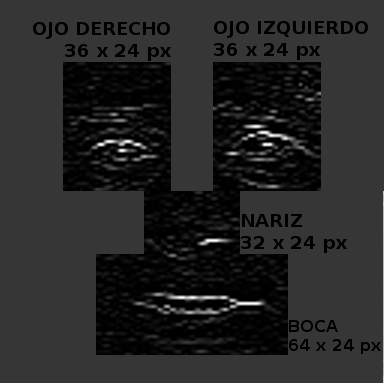
\includegraphics[width=8cm]{zonas_busqueda_cara.png}
	\caption{Máscara aplicada sobre la imagen y tamaños de ventana}
	\label{fig:imagen_mascaras}
\end{figure}

Tras la detección de esquinas, procedemos a la búsqueda de los ojos, nariz y boca. Para ello, buscamos en el resultante de aplicar la máscara de la figura \ref{fig:imagen_mascaras} un algoritmo para buscar la ventana del tamaño indicado con suma de mayor valor. La búsqueda se realiza en el eje vertical de la imagen. Informalmente, buscamos la ventana de tamaño WxH (indicados en la imagen) cuyo valor de sumatorio sea el máximo. Formalmente, la región K es la resultante de la máscara que aparece en la imagen y se expresaría de la siguiente manera:
\[
 K = \left( 
	\begin{array}{lcccr} 
		k_{0,0} & k_{0,1} & \hdots & k_{0,j-2} & k_{0,j-1} \\
		\vdots & \vdots & \ddots & \vdots & \vdots \\
		k_{i-1,0} & k_{i-1,1} & \hdots & k_{i-1,j-2} & k_{i-1,j-1} \\
	\end{array} \right)
\]
Y que buscamos el valor de m según la siguiente ecuación. El sumatorio de la submatriz [(0,m), (W,m+H)] tendrá el valor máximo de la máscara indicada.
\[
   V = K\left[\left(0,m\right), \left(W,m+H\right) \right] \mid \forall n \sum_{i=0,j=n}^{i=W,j=n+H} K_{i,j} \leq \sum_{p=0,q=m}^{p=W,q=m+H} K_{p,q} 
\]
Este método se ha mostrado fiable, rápido y paralelizable (búsqueda de ambos ojos y nariz como tres hilos de ejecución diferentes, y tras el resultado de la detección de la nariz se puede realizar la búsqueda de la boca) aunque se ha reconocido casos en los que puede dar problemas. En la figura \ref{fig:imagenes_procesadas} podemos observar:
\begin{itemize}
	\item{A la izquierda la imagen original en color, con la región en la que se ha detectado la cara encuadrada.}
	\item{A la derecha, la primera imagen desde arriba es la cara detectada tras aplicar la conversión a escala de grises y el redimensionado bilinear.}
	\item{Bajo la anterior, está la imagen resultante de la aplicación del detector de esquinas Sobel de segundo orden sobre el eje Y.}
	\item{Por debajo de la anterior, tenemos encuadradas las máximas ventanas según los criterios previamente señalados.}
	\item{Finalmente, la imagen inferior de la derecha es el resultado de aplicar las ventanas halladas sobre la cara en escala de grises y redimensionada}
\end{itemize}
\begin{figure}[h!]
	\centering
	%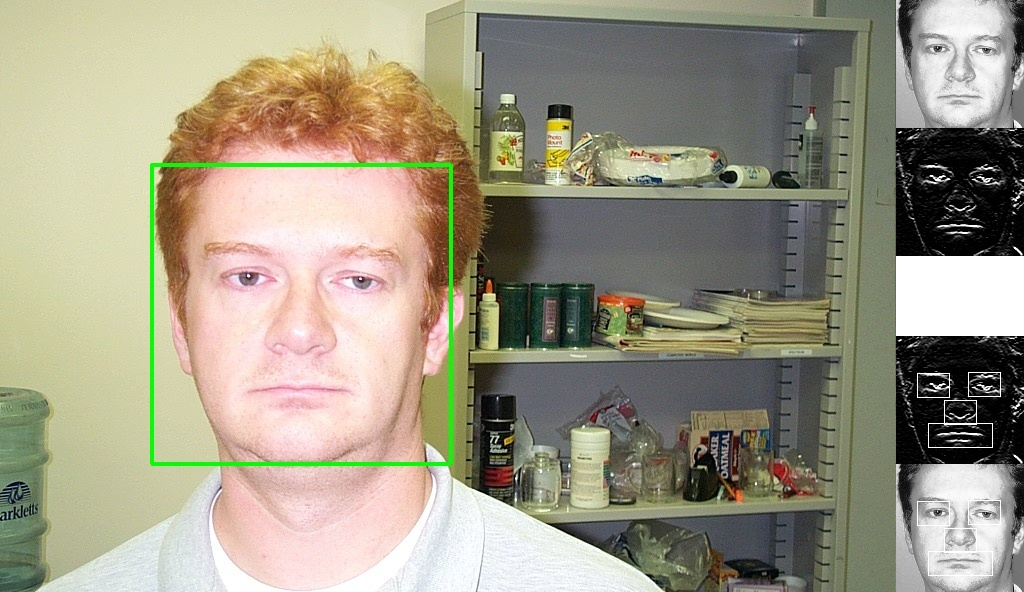
\includegraphics[height=7cm]{ejemplo_imagen_hombre.jpg}
	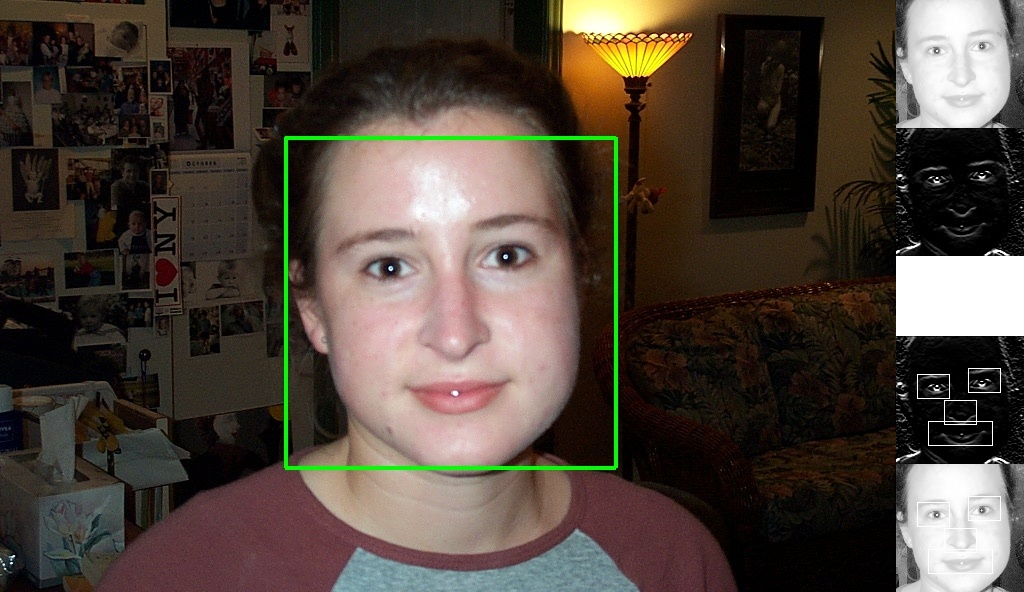
\includegraphics[width=12cm]{ejemplo_imagen_mujer.jpg}
	\caption{Pasos del procesado de la imagen}
	\label{fig:imagenes_procesadas}
\end{figure}
%si esto cuela y lo explico bien, doy volteretas

\section{Extracción de características}
Con lo que hemos podido obtener hasta ahora, toca pasar la imagen por un banco de filtros de Gabor... 

\subsection{Identificación}

\section{Comparación entre huellas faciales}
Las medidas que se pueden aplicar de distancias entre ...
